\documentclass[11pt,twoside]{article}


\usepackage{fancyhdr}\pagestyle{fancy}
\fancyhf{}
\rhead{OpenBDLM V1.0 reference manual}
\lhead{\leftmark}
\cfoot{\thepage}


\usepackage{pdfpages}

%FAQ
\usepackage{lipsum}
\newcounter{question}
\setcounter{question}{0}

%\usepackage[section]{placeins}


\usepackage{placeins}

\let\Oldsection\section
\renewcommand{\section}{\FloatBarrier\Oldsection}

\let\Oldsubsection\subsection
\renewcommand{\subsection}{\FloatBarrier\Oldsubsection}

\let\Oldsubsubsection\subsubsection
\renewcommand{\subsubsection}{\FloatBarrier\Oldsubsubsection}


% bibliography
\usepackage[numbers]{natbib}

% MATLAB code package
\usepackage{listings}
\usepackage[framed]{matlab-prettifier}
\usepackage[T1]{fontenc}
\definecolor{light-gray}{gray}{0.95}
\definecolor{matlab-yellow}{RGB}{252,251,220}

\usepackage{upquote}
\usepackage{xspace}
\usepackage{graphicx}

\usepackage{todonotes}
\usepackage{microtype}


% For math symbol, equations, etc...
\RequirePackage{amsmath}
\RequirePackage{amsfonts}
\RequirePackage{amssymb}
\RequirePackage{latexsym}
\RequirePackage{amscd}
\RequirePackage{mathtools}
\RequirePackage{bm}

\usepackage{mathabx}

\usepackage{hyperref}
\hypersetup{colorlinks=true,linkcolor=blue}

\usepackage{subcaption} 
\usepackage[capitalise,noabbrev]{cleveref}

% For table
\usepackage{booktabs}
\usepackage{multirow}
\usepackage{array}
\newcommand{\xbar}[1]{\overline{#1}}
\newcolumntype{L}[1]{>{\raggedright\arraybackslash}m{#1}} 
\newcolumntype{C}[1]{>{\centering\arraybackslash}m{#1}} 
\newcolumntype{R}[1]{>{\raggedleft\arraybackslash}m{#1}} 
\newcolumntype{N}{@{}m{0pt}@{}}

\usepackage{longtable}

\makeatletter
\newcommand{\thickhline}{%
    \noalign {\ifnum 0=`}\fi \hrule height 1pt
    \futurelet \reserved@a \@xhline
}
\newcolumntype{"}{@{\hskip\tabcolsep\vrule width 1pt\hskip\tabcolsep}}
\makeatother


% For description
\usepackage{enumitem}
\setlist[description]{%
  topsep=30pt,               % space before start / after end of list
  itemsep=5pt,               % space between items
  font={\normalfont\textbullet\space}, % set the label font
}

% For rotating figures, tables, etc.  including their captions
\usepackage[figureleft]{rotating}

%%%%%%%%%%%%%%%%%%%%%%%%%%%%
%TIKZ PACKAGE
%%%%%%%%%%%%%%%%%%%%%%%%%%%%
\usepackage{tikz}
\usetikzlibrary{calc,patterns,decorations.pathmorphing,decorations.markings,decorations.pathreplacing}
\usetikzlibrary{shapes,fit}
\usetikzlibrary{positioning}
\usetikzlibrary{matrix}
\usetikzlibrary{decorations.text}
%\usetikzlibrary{decorations.markings}
\usetikzlibrary{shapes.geometric,arrows,positioning}
\usetikzlibrary{positioning,arrows.meta,bending}
%Rectangle
\tikzstyle{rect}=[rectangle, minimum width=2.2cm,minimum height=1.2cm,draw=black!100, thick]
\tikzstyle{wrect}=[rectangle, minimum width=2.2cm,minimum height=1.2cm,draw=white!100, thick]
\tikzstyle{smallrect}=[rectangle, minimum width=1cm,minimum height=0.5cm,draw=black!100, thick]
\tikzstyle{smallrectm}=[rectangle, minimum width=1.5cm,minimum height=0.5cm,draw=black!100, thick]
\tikzstyle{PCA}=[rectangle, minimum width=2.2cm,minimum height=1.2cm,draw=red!100, very thick,rounded corners]
\tikzstyle{user}=[circle,draw, inner sep = 1.5pt]
\tikzstyle{eslightgray}=[rectangle, draw=black!100, thick,fill opacity=0.5, text opacity=1, fill=lightgray, minimum height = 1cm, inner sep=0pt]
\tikzstyle{esaliceblue}=[rectangle, draw=black!100, thick, fill=aliceblue, minimum height = 1cm, inner sep=0pt]
\tikzstyle{esbabyblueeyes}=[rectangle, draw=black!100, thick, fill=babyblueeyes, minimum height = 1cm, inner sep=0pt]
\tikzstyle{esbabyblueeyestransp}=[rectangle, draw=black!100, thick fill=babyblueeyes, fill opacity=0.2, text opacity=1,  minimum height = 1cm, inner sep=0pt]
\tikzstyle{esbisque}=[rectangle, draw=black!100, thick, fill=bisque, minimum height = 1cm, inner sep=0pt, fill opacity=0.5, text opacity=1]
\tikzstyle{esbisquetransp}=[rectangle, draw=black!100, thick, fill=bisque, fill opacity=0.5, text opacity=1, minimum height = 1cm, inner sep=0pt]
\tikzstyle{esceladon}=[rectangle, draw=black!100, thick, fill=celadon, minimum height = 1cm, inner sep=0pt]
\tikzstyle{eswhite}=[rectangle, draw=black!100, thick, fill=white, minimum height = 1cm, inner sep=0pt, draw=black!100, thick]
\tikzstyle{esamber}=[rectangle, draw=black!100, thick, fill=amber, minimum height = 1cm, inner sep=0pt, draw=black!100,  thick]
\tikzstyle{esbrightlavender}=[rectangle, draw=black!100, thick, fill=brightlavender, minimum height = 1cm, inner sep=0pt, draw=black!100,  thick]
\tikzstyle{para}=[trapezium ,minimum height=0.8 cm, draw=black!100, thick, trapezium left angle=-120, trapezium right angle=-60,trapezium stretches, inner sep = 0pt]
\tikzstyle{paraamber}=[trapezium , fill=amber, minimum height=0.8 cm, draw=black!100, thick, trapezium left angle=-120, trapezium right angle=-60,trapezium stretches, inner sep = 0pt]
\tikzstyle{parababyblueeyes}=[trapezium , fill=babyblueeyes, minimum height=0.8 cm, draw=black!100, thick, trapezium left angle=-120, trapezium right angle=-60,trapezium stretches, inner sep = 0pt]
\tikzstyle{paraambertransp}=[trapezium , fill=amber, minimum height=0.8 cm, draw=black!100, thick, fill opacity=0.2, text opacity=1, trapezium left angle=-120, trapezium right angle=-60,trapezium stretches, inner sep = 0pt]
\tikzstyle{paraceladon}=[trapezium , fill=celadon, minimum height=0.8 cm, draw=black!100, thick, trapezium left angle=-120, trapezium right angle=-60,trapezium stretches, inner sep = 0pt]
\tikzstyle{parabisque}=[trapezium , fill=bisque, minimum height=0.8 cm, draw=black!100, thick,  fill opacity=0.5, text opacity=1, trapezium left angle=-120, trapezium right angle=-60,trapezium stretches, inner sep = 0pt]
\tikzstyle{paralightgray}=[trapezium , fill=lightgray, minimum height=0.8 cm, draw=black!100, thick,  fill opacity=0.5, text opacity=1, trapezium left angle=-120, trapezium right angle=-60,trapezium stretches, inner sep = 0pt]
\tikzstyle{parawhite}=[trapezium , fill=white, minimum height=0.8 cm, draw=black!100, thick,  fill opacity=0.5, text opacity=1, trapezium left angle=-120, trapezium right angle=-60,trapezium stretches, inner sep = 0pt]

% Parallelogram
\tikzstyle{para}=[trapezium, minimum width=3cm,minimum height=1.2cm, draw=black!100,  thick, trapezium left angle=-150, trapezium right angle=-30,trapezium stretches]
%Hexagone in text
\tikzstyle{hexa}=[signal, signal to=left and right, minimum width=4cm,minimum height=1.2cm, draw=black!100, thick]

 \tikzstyle{user}=[circle,draw, inner sep = 1.5pt]
 \tikzstyle{test}=[diamond, aspect=1, minimum width=1.5cm, minimum height = 1.5cm, draw=black!100, thick,  inner sep=-1pt]
 \tikzstyle{testamber}=[diamond, fill=amber, aspect=1, minimum width=1.5cm, minimum height = 1.5cm, draw=black!100, thick,  inner sep=-1pt]
 \tikzstyle{testbabyblueeyes}=[diamond, fill=babyblueeyes, aspect=1, minimum width=1.5cm, minimum height = 1.5cm, draw=black!100, thick,  inner sep=-1pt]
 \tikzstyle{testbisque}=[diamond, fill=bisque, aspect=1, minimum width=1.5cm, minimum height = 1.5cm, draw=black!100, thick,  inner sep=-1pt, fill opacity=0.5, text opacity=1]
 \tikzstyle{testceladon}=[diamond, fill=celadon, aspect=1, minimum width=1.5cm, minimum height = 1.5cm, draw=black!100, thick,  inner sep=-1pt]
 \tikzstyle{testlightgray}=[diamond, fill=lightgray, aspect=1, minimum width=1.5cm, minimum height = 1.5cm, fill opacity=0.5, text opacity=1, draw=black!100, thick,  inner sep=-1pt]
  \tikzstyle{testwhite}=[diamond, fill=white, aspect=1, minimum width=1.5cm, minimum height = 1.5cm, draw=black!100, thick,  inner sep=-1pt]
 
%Connecting link
\tikzstyle{connect}=[-latex, thick,>=latex]
\tikzstyle{shaded}=[draw=black!20,fill=black!20]
\tikzstyle{line} = [draw, -latex,thick,>=latex]

\definecolor{egg}{RGB}{250,250,235}
\definecolor{aliceblue}{rgb}{0.94, 0.97, 1.0}
\definecolor{babyblueeyes}{rgb}{0.63, 0.79, 0.95}
\definecolor{bisque}{rgb}{0.91, 0.45, 0.32}
\definecolor{celadon}{rgb}{0.67, 0.88, 0.69}
\definecolor{amber}{rgb}{1.0, 0.99, 0.82}%{1.0, 0.75, 0.0}
\definecolor{brightlavender}{rgb}{0.75, 0.58, 0.89}

\graphicspath{{./docfigs/}}


\title{
\includegraphics[width=100mm]{OpenBDLM_logo.pdf}\\[20pt]
 OpenBDLM V1.0 reference manual}
\author{Ianis Gaudot, Luong Ha Nguyen, and James-A. Goulet \\ Polytechnique Montreal}

\begin{document}

\newcommand{\MATLAB}{\textsc{Matlab}}


\newcommand\Que[1]{%
   \leavevmode\par
   \stepcounter{question}
   \noindent
   \thequestion. Q --- #1\par}

\newcommand\Ans[2][]{%
    \leavevmode\par\noindent
   {\leftskip37pt
    A --- \textbf{#1}#2\par}}


\maketitle

\tableofcontents
\newpage

\section{Getting started}

\subsection{What is OpenBDLM ?}
\label{S:OPENBDLMWHATIS}

OpenBDLM is a \MATLAB{} open-source software developed to use Bayesian Dynamic Linear Models for long-term time series analysis (i.e time step in the order of one hour or higher).
OpenBDLM is capable of processing simultaneously several time series, enabling interpretation, monitoring and prediction over time.
OpenBDLM includes an anomaly detection tool which allows detecting abnormal behavior in a fully probabilistic framework.
In addition, OpenBDLM handles time series with missing data and non-uniform timestep vector.
OpenBDLM is available for download from GitHub at \url{https://github.com/CivML-PolyMtl/OpenBDLM}.\\

\noindent \textbf{Keywords}: time series analysis and forecasting, linear gaussian state-space models, time-series decomposition, anomaly detection, filtering, smoothing, bayesian analysis.

\subsection{Installing OpenBDLM}
\label{S:OPENBDLMINSTALLING}

The following instructions show how to download and setup OpenBDLM on your local machine for direct use, testing, and development purposes.
\subsubsection{Prerequisites}
\MATLAB{} (version 2016a or higher) installed on Mac OSX or Windows.\\

\noindent
The \MATLAB{}  \emph{Statistics and Machine Learning Toolbox} is required.

\subsubsection{Installation}
\begin{enumerate}
\item If an older OpenBDLM version is already installed, it is recommanded to remove from your \MATLAB{} path any previous OpenBDLM versions.
\item Download and extract the ZIP file from \url{https://github.com/CivML-PolyMtl/OpenBDLM} (or clone the git repository) in your working directory.
\item Add ``OpenBDLM-master'' folder and all its subfolders to your \MATLAB{}  path through one of the following two options:
\begin{itemize}
    \item using the ``Set Path'' dialog box in \MATLAB{}, or 
    \item by running  \lstinline[basicstyle = \mlttfamily \small, backgroundcolor = \color{light-gray}]!addpath! function from the \MATLAB{} command window
    \end{itemize}
\end{enumerate}


\subsection{Starting OpenBDLM}
\label{S:OPENBDLMGETTINGSTARTED}

\begin{itemize}
\item Set the current working directory to the folder ``OpenBDLM-master''
%\begin{center}
\item Type \colorbox{light-gray}{\lstinline[basicstyle = \mlttfamily \small, backgroundcolor = \color{light-gray}]!OpenBDLM_main;!}, and press the key enter $\dlsh$.
%\end{center}
in the \MATLAB{} command line.
\end{itemize}
The OpenBDLM starting menu should appear on the \MATLAB{} command window (see Listing~\ref{LST:OpenBDLMStartingMenu}).
Type \colorbox{light-gray}{\lstinline[basicstyle = \mlttfamily \small, backgroundcolor = \color{light-gray}]!Q!} in the command line, and press the key enter $\dlsh$ to quit the program.
%\begin{lstlisting}[ frame = single, basicstyle = \mlttfamily \small, backgroundcolor = \color{light-gray}, linewidth=\linewidth] %, caption = OpenBDLM call ]%, label = LST:OpenBDLMmain, captionpos=b]
%[data, model, estimation, misc] = OpenBDLM_main();
%\end{lstlisting}
\begin{lstlisting}[ frame = single, basicstyle = \mlttfamily \small, caption = {OpenBDLM starting menu on  \MATLAB{} command window when calling \lstinline!OpenBDLM\_main;!}, label = LST:OpenBDLMStartingMenu ,  float =ht, linewidth=\linewidth, captionpos=b]

------------------------------------------------
     Starting OpenBDLM_V1.0
------------------------------------------------
            Time series analysis using 
            Bayesian Dynamic Linear Models
------------------------------------------------
- Start a new project: 

     *      Enter a configuration filename 
     0   -> Interactive tool 

- Type D to Delete project(s), V for Version control, Q to Quit.

     choice >>
\end{lstlisting}


\subsection{Demo}

In the \MATLAB{} command line, type  
%\begin{lstlisting}[frame = single, basicstyle = \mlttfamily \small, backgroundcolor = \color{light-gray}, caption = Run the OpenBDLM demo, label = LST:OpenBDLMdemo, captionpos=b, linewidth=\linewidth]
%run_DEMO.m
%\end{lstlisting}
%\begin{center}
\colorbox{light-gray}{\lstinline[basicstyle = \mlttfamily \small, backgroundcolor = \color{light-gray}]!run_DEMO;! }
%\end{center}
 followed by pressing the key enter $\dlsh$ to run a demo. 
%\lstinline[basicstyle = \mlttfamily \small, backgroundcolor = \color{light-gray}]!run_DEMO.m! to run a little demo. 
Some messages on the \MATLAB{} command window show that the program has started (see Listing~\ref{LST:MessageDemo}).
Some figures as shown in Figure~\ref{fig:DataSummaryRaw4}, and Figure~\ref{fig:SYNTHETICOptimizedOptimizedExample4} should popup on the screen \footnote{The demo runs in batch the example described in Section~\ref{S:EXAMPLESYNTHETICDATA}.}


\begin{lstlisting}[frame = single, basicstyle = \mlttfamily \small, caption = {Output on \MATLAB{} command window when running \lstinline!run_DEMO.m!}, linewidth=\linewidth, label=LST:MessageDemo, ,captionpos=b, float = h] 
     Starting OpenBDLM_V1.0...
     Starting a new project...
     Building model...
     Simulating data...
     Plotting data...
     Saving database (binary format) ...
     Saving database (csv format) ...
     Saving project...
     Printing configuration file...
     Saving database (binary format) ...
     Saving project...
     Done ! See you soon !
\end{lstlisting}



\subsection{OpenBDLM main menu}
\label{S:OPENBDLMMAINMENU}

Once a project is loaded, the OpenBDLM main menu displays the list of actions which can be done (see Listing~\ref{LST:OpenBDLMMainMenu}). 
The OpenBDLM main menu appears each time a selected action is done; until the user types \colorbox{light-gray}{\lstinline[basicstyle = \mlttfamily \small ]!Q!} to save the project and quit the program.

%\begin{itemize}
%    \item option  \colorbox{light-gray}{\lstinline[basicstyle = \mlttfamily \small ]!1!}: estimates the model parameters
%    \item option  \colorbox{light-gray}{\lstinline[basicstyle = \mlttfamily \small ]!2!}: estimates the initial hidden states
%    \item option  \colorbox{light-gray}{\lstinline[basicstyle = \mlttfamily \small ]!3!}: estimate the hidden states
%    \item option  \colorbox{light-gray}{\lstinline[basicstyle = \mlttfamily \small ]!11!}: display the current model parameters values on the \MATLAB{} command line window and allows the user to modify the model parameters values
%     \item option  \colorbox{light-gray}{\lstinline[basicstyle = \mlttfamily \small ]!12!}: display the initial hidden states values on the \MATLAB{} command line window and allows the user to modify the initial hidden states values
%     \item option  \colorbox{light-gray}{\lstinline[basicstyle = \mlttfamily \small ]!13!}: display information about the current training period  on the \MATLAB{} command line window and allows the user to modify the training period
%     \item option  \colorbox{light-gray}{\lstinline[basicstyle = \mlttfamily \small ]!14!}: plot figures on the screen about the data in memory, the data availability, and the hidden states estimation results
%     \item option  \colorbox{light-gray}{\lstinline[basicstyle = \mlttfamily \small ]!15!}: display the content of the model matrices on the \MATLAB{} command line window at a specific time
%     \item option  \colorbox{light-gray}{\lstinline[basicstyle = \mlttfamily \small ]!16!}: create synthetic data from the current information in memory
%     \item option  \colorbox{light-gray}{\lstinline[basicstyle = \mlttfamily \small ]!17!}: export data and results as well as the figures in PNG, PDF and  \LaTeX{}   format
%     \item option  \colorbox{light-gray}{\lstinline[basicstyle = \mlttfamily \small ]!18!}: display the current options 
%    \end{itemize}

\begin{lstlisting}[ frame = single, basicstyle = \mlttfamily \small, caption = { OpenBLDM main menu}, label = LST:OpenBDLMMainMenu,  float =h!, linewidth=\linewidth, captionpos=b]
---------------------------------------------
/    OpenBDLM main menu. Choose from 
--------------------------------------------- 

     1  ->  Learn model parameters values 
     2  ->  Estimate initial hidden states values 
     3  ->  Estimate hidden states values 

     11 ->  Display and modify current model parameter values 
     12 ->  Display and modify current initial hidden states values 
     13 ->  Display and modify current training period 
     14 ->  Plots 
     15 ->  Display model matrices 
     16 ->  Create synthetic data 
     17 ->  Export
     18 ->  Display current options in configuration file format 

     Type Q to Save and Quit 

     choice >> 
\end{lstlisting}






\section{Inputs and outputs}
\label{S:OpenBDLMINPUTOUTPUT}

\subsection{Inputs}
\label{SS:OpenBDLMinput}


OpenBDLM has two operating modes: \emph{interactive mode} and \emph{batch mode}. In the \emph{interactive mode}, OpenBDLM takes the required input for the project through \MATLAB{} command line queries. Each input is validated after pressing the Enter key $\dlsh$. In \emph{batch mode}, the inputs are provided in advance by the user and stored in a cell array of characters vector. OpenBDLM reads sequentially the inputs and performs the analysis. The batch mode requires the user to be familiar with the interactive mode because the set of inputs must be provided prior to the analysis. {\lstinline[basicstyle = \mlttfamily \small]!OpenBDLM_main! can take three types of input:
\begin{itemize}
  \item no input (\emph{interactive mode}) \\ 
  
  \colorbox{light-gray}{\lstinline[basicstyle = \mlttfamily \small]!OpenBDLM_main;!} \\  
  %the program requests user's inputs from the command line. 
  \item the name of configuration file given as a character vector  (\emph{interactive mode}) \\ 
  
    \colorbox{light-gray}{\lstinline[basicstyle = \mlttfamily \small]!OpenBDLM_main('CFG_DEMO.m');!} \\ 
      
    %a configuration file (see Section~\ref{S:CFGFile}) is used to initialize the project
  \item a cell array of character vectors  (\emph{batch mode}) \\
  
\raggedright{\colorbox{light-gray}{\lstinline[basicstyle = \mlttfamily \small]!OpenBDLM_main(\{'''CFG_DEMO.m''', '2', '3', '1', '''Q'''\});!}} \\
 %the program reads pre-loaded commands stored in an input cell-array of character vectors.
\end{itemize}

\subsection{Outputs}

 Four possible outputs can be obtained from \lstinline[basicstyle = \mlttfamily \small]!OpenBDLM_main.m!.
 These outputs are \lstinline[basicstyle = \mlttfamily \small ]!data!, \lstinline[basicstyle = \mlttfamily \small ]!model!, \lstinline[basicstyle = \mlttfamily \small ]!estimation!, and \lstinline[basicstyle = \mlttfamily \small ]!misc!.\\
 
 \raggedright{\colorbox{light-gray}{\lstinline[basicstyle = \mlttfamily \small]![data, model, estimation, misc]=OpenBDLM_main;!}} \\

\subsubsection{data} 

The output variable \lstinline[basicstyle = \mlttfamily \small]!data! stores the time series used for the analysis. 
The timestamps values, the amplitude values and the label values are stored in the fields \lstinline[basicstyle = \mlttfamily \small ]!timestamps!, \lstinline[basicstyle = \mlttfamily \small ]!values!, and \lstinline[basicstyle = \mlttfamily \small ]!labels!, respectively.
\begin{itemize}
\item \lstinline[basicstyle = \mlttfamily \small ]!labels!:  See Section~\ref{SS:MATInput} for details.
\item \lstinline[basicstyle = \mlttfamily \small ]!timestamps!:  See Section~\ref{SS:MATInput} for details.
\item \lstinline[basicstyle = \mlttfamily \small ]!values!:  See Section~\ref{SS:MATInput} for details.
\end{itemize}

\subsubsection{model}
The output variable \lstinline[basicstyle = \mlttfamily \small]!model! stores all the information related to the model used in the analysis. 
This variables has 14 fields, amongst them are \lstinline[basicstyle = \mlttfamily \small ]!hidden_states_names!, \lstinline[basicstyle = \mlttfamily \small ]!A!, \lstinline[basicstyle = \mlttfamily \small ]!C!, \lstinline[basicstyle = \mlttfamily \small ]!Q!, \lstinline[basicstyle = \mlttfamily \small ]!R!, \lstinline[basicstyle = \mlttfamily \small ]!Z!, \lstinline[basicstyle = \mlttfamily \small ]!components!, \lstinline[basicstyle = \mlttfamily \small ]!parameter_properties!, \lstinline[basicstyle = \mlttfamily \small ]!initX!, \lstinline[basicstyle = \mlttfamily \small ]!initV!, \lstinline[basicstyle = \mlttfamily \small ]!initS!.


\begin{itemize}
\item \lstinline[basicstyle = \mlttfamily \small ]!hidden_states_names!:  this field stores a $1\times \mathtt{S}$ cell array, where $\mathtt{S} = \{1,2 \}$ is the number of model classes.
Each cell array is a $ \mathtt{L} \times 3$ cell array, where $\mathtt{L}$ is the number of hidden states. The first column of the cell array stores the reference name of the hidden state, the second column indicate the index of the model class to which the hidden state belongs and the third column indicates the index of the time series to which the hidden states belongs.
\item \lstinline[basicstyle = \mlttfamily \small ]!A!:  this field stores $1\times \mathtt{S}$ cell array, where $\mathtt{S} = \{1,2 \}$ is the number of model classes. The cell array contains function handles used to build the full transition matrix.
\item \lstinline[basicstyle = \mlttfamily \small ]!C!:  this field stores $1\times \mathtt{S}$ cell array, where $\mathtt{S} = \{1,2 \}$ is the number of model classes. The cell array contains function handles used to build the full observation matrix.
\item \lstinline[basicstyle = \mlttfamily \small ]!Q!: this field stores $1\times \mathtt{S}$ cell array, where $\mathtt{S} = \{1,2 \}$ is the number of model classes. The cell array contains function handles used to build the full process noise covariance matrix.
\item \lstinline[basicstyle = \mlttfamily \small ]!R!:  this field stores $1\times \mathtt{S}$ cell array, where $\mathtt{S} = \{1,2 \}$ is the number of model classes. The cell array contains function handles used to build the full observation noise covariance matrix.
\item \lstinline[basicstyle = \mlttfamily \small ]!Z!:  this field stores a function handle used to build the transition probabilities matrix.
\item \lstinline[basicstyle = \mlttfamily \small ]!components!:   See Section~\ref{SS:ModelComponents} for details.
\item \lstinline[basicstyle = \mlttfamily \small ]!parameter_properties!: See Section~\ref{SS:ModelParamProperties} for details.
\item \lstinline[basicstyle = \mlttfamily \small ]!initX!: See Section~\ref{SS:InitialHS} for details.
\item \lstinline[basicstyle = \mlttfamily \small ]!initV!: See Section~\ref{SS:InitialHS} for details.
\item \lstinline[basicstyle = \mlttfamily \small ]!initS!: See Section~\ref{SS:InitialHS} for details.
\end{itemize}


\subsubsection{estimation} 
The \lstinline[basicstyle = \mlttfamily \small ]!estimation! structure stores the filtered or smoothed hidden states results.
This variable has 11 fields, among them  are \lstinline[basicstyle = \mlttfamily \small ]!x!, \lstinline[basicstyle = \mlttfamily \small ]!V!, \lstinline[basicstyle = \mlttfamily \small ]!y!, \lstinline[basicstyle = \mlttfamily \small ]!Vy!,  \lstinline[basicstyle = \mlttfamily \small ]!S!, \lstinline[basicstyle = \mlttfamily \small ]!LL!, \lstinline[basicstyle = \mlttfamily \small ]!x_M!, \lstinline[basicstyle = \mlttfamily \small ]!V_M!, \lstinline[basicstyle = \mlttfamily \small ]!VV_M!.

\begin{itemize}
\item \lstinline[basicstyle = \mlttfamily \small ]!x!: this field stores the mean of the estimated hidden states. \lstinline[basicstyle = \mlttfamily \small ]!x! stores a $\mathtt{L} \times \mathtt{T}$ array, where $\mathtt{L}$ and $\mathtt{T}$ are the number of hidden states and the length of time vector, respectively. 
\item \lstinline[basicstyle = \mlttfamily \small ]!V!: this field stores the variance of the estimated hidden states. \lstinline[basicstyle = \mlttfamily \small ]!V! stores a $\mathtt{L} \times \mathtt{T}$ array, where $\mathtt{L}$ and $\mathtt{T}$ are the number of hidden states and the length of time vector, respectively. 
\item \lstinline[basicstyle = \mlttfamily \small ]!y!: this field stores the mean of the estimated system responses. \lstinline[basicstyle = \mlttfamily \small ]!y! stores a $\mathtt{D} \times \mathtt{T}$ array, where $\mathtt{D}$ and $\mathtt{T}$ are the number of time-series and the length of time vector, respectively. 
\item \lstinline[basicstyle = \mlttfamily \small ]!Vy!: this field stores the variance of the estimated system responses. \lstinline[basicstyle = \mlttfamily \small ]!Vy! stores a $\mathtt{D} \times \mathtt{T}$ array, where $\mathtt{D}$ and $\mathtt{T}$ are the number of time-series and the length of time vector, respectively. 
\item \lstinline[basicstyle = \mlttfamily \small ]!S!: this field stores the probability of each model class. \lstinline[basicstyle = \mlttfamily \small ]!S! stores a $\mathtt{T} \times \mathtt{S}$ array, where $\mathtt{D}$ and $\mathtt{S}$ are the number of time-series and the number of model classes, respectively. 
\item \lstinline[basicstyle = \mlttfamily \small ]!LL!: this field stores the value of the log-likelihood.
\item \lstinline[basicstyle = \mlttfamily \small ]!x_M!: this field stores the mean of the estimated hidden states for each model class before the merging step. \lstinline[basicstyle = \mlttfamily \small ]!x_M! stores a $1 \times \mathtt{S}$ cell array, where  where $\mathtt{S} = \{1,2 \}$ is the number of model classes. Each cell array stores a $\mathtt{L} \times \mathtt{T}$ array, where $\mathtt{L}$ and $\mathtt{T}$ are the number of hidden states and the length of time vector, respectively.
\item \lstinline[basicstyle = \mlttfamily \small ]!V_M!: this field stores the variance and covariance of the estimated hidden states for each model class before the merging step. \lstinline[basicstyle = \mlttfamily \small ]!V_M! stores $1 \times \mathtt{S}$ cell array, where $\mathtt{S} = \{1,2 \}$ is the number of model classes. Each cell array stores $\mathtt{L} \times  \mathtt{L} \times \mathtt{T}$ array, where $\mathtt{L}$ and $\mathtt{T}$ are the number of hidden states and the length of time vector, respectively.
\end{itemize}

\subsubsection{misc}
The \lstinline[basicstyle = \mlttfamily \small ]!misc! structure stores the options and internal variables needed for running the software.
This variable has 3 fields, amongst them \lstinline[basicstyle = \mlttfamily \small ]!ProjectName!, \lstinline[basicstyle = \mlttfamily \small ]!internalVars!, \lstinline[basicstyle = \mlttfamily \small ]!options!.

\begin{itemize}
\item \lstinline[basicstyle = \mlttfamily \small ]!ProjectName!: this field stores the name of the project as a character array.
\item \lstinline[basicstyle = \mlttfamily \small ]!internalVars!: this field stores internal variables which are needed for running the software.
\item \lstinline[basicstyle = \mlttfamily \small ]!options!: this field stores the options that control different aspects of the software. The list of options is given in Section~\ref{SS:options}.
\end{itemize}


\subsection{OpenBDLM files types}
OpenBDLM reads and/or creates five types of files: \lstinline[basicstyle = \mlttfamily \small]!DATA_!, \lstinline[basicstyle = \mlttfamily \small ]!CFG_!, \lstinline[basicstyle = \mlttfamily \small ]!PROJ_!, \lstinline[basicstyle = \mlttfamily \small ]!RES_! and \lstinline[basicstyle = \mlttfamily \small ]!LOG_!.
\begin{itemize}
    \item \lstinline[basicstyle = \mlttfamily \small ]!DATA_! files: the files named with the prefix \lstinline[basicstyle = \mlttfamily \small ]!DATA_! are \MATLAB{} MAT binary files that store the time series data (see Section~\ref{SS:MATInput}). These files are located in the ``data/mat'' subfolder.
    \item  \lstinline[basicstyle = \mlttfamily \small ]!CFG_! files: the files named with the prefix \lstinline[basicstyle = \mlttfamily \small ]!CFG_! are  \MATLAB{} scripts used to initialize and export a project (see Section~\ref{S:CFGFile}). These files are located in the ``config\_files'' subfolder.
    \item  \lstinline[basicstyle = \mlttfamily \small ]!PROJ_! files: the files named with the prefix \lstinline[basicstyle = \mlttfamily \small ]!PROJ_! are \MATLAB{} MAT binary files that stores a full project for further analysis. These files are located in the ``saved\_projects'' subfolder.
    \item \lstinline[basicstyle = \mlttfamily \small ]!RES_!  files: the files named with the prefix \lstinline[basicstyle = \mlttfamily \small ]!RES_! are \MATLAB{} MAT binary files that stores the estimation results. These files are located in the ``results/mat'' subfolder.
    \item \lstinline[basicstyle = \mlttfamily \small ]!LOG_! files: the files named with the prefix \lstinline[basicstyle = \mlttfamily \small ]!LOG_! are plain TEXT files that record events occurring during the program run. These files are located in the ``log\_files'' subfolder.
\end{itemize}



\section{Modes}
\label{S:OPENBDLMRUNNINGMODES}

\subsection{Interactive mode}
\label{SS:InteractiveMode}

In interactive mode, OpenBDLM takes the required input for the project through \MATLAB{} command line queries.
% requests and reads input from the user.
%The input must be provided from the keyboard and be typed in the Matlab command line.
Each input is validated after pressing the Enter key $\dlsh$.

\subsection{Batch mode}
\label{SS:Batchmode}

In batch mode, the inputs are provided in advance by the user and stored in a cell array of characters vector.
OpenBDLM reads sequentially the inputs and performs the analysis.  %silently as requested from the inputs.
The batch mode requires the user to be familiar with the interactive mode because the set of input must be provided prior to the analysis.

\section{Configuration file}
\label{S:CFGFile}
The configuration file is a \MATLAB{} script utilized for initializing the project (see Figure \ref{fig:cfgfile}).
The name of a configuration file can be given as an input to the function   \lstinline[basicstyle = \mlttfamily \small ]!OpenBLDM_main.m!, as mentionned in Section~\ref{SS:OpenBDLMinput}.
The configuration file must follow a specific structures, which includes 6 sections: Project name, Data, Model structure, Model parameters, Initial states values and Options.
The first three sections are mandatory, while the last three sections are optional.
\begin{figure}[h!]
\centering
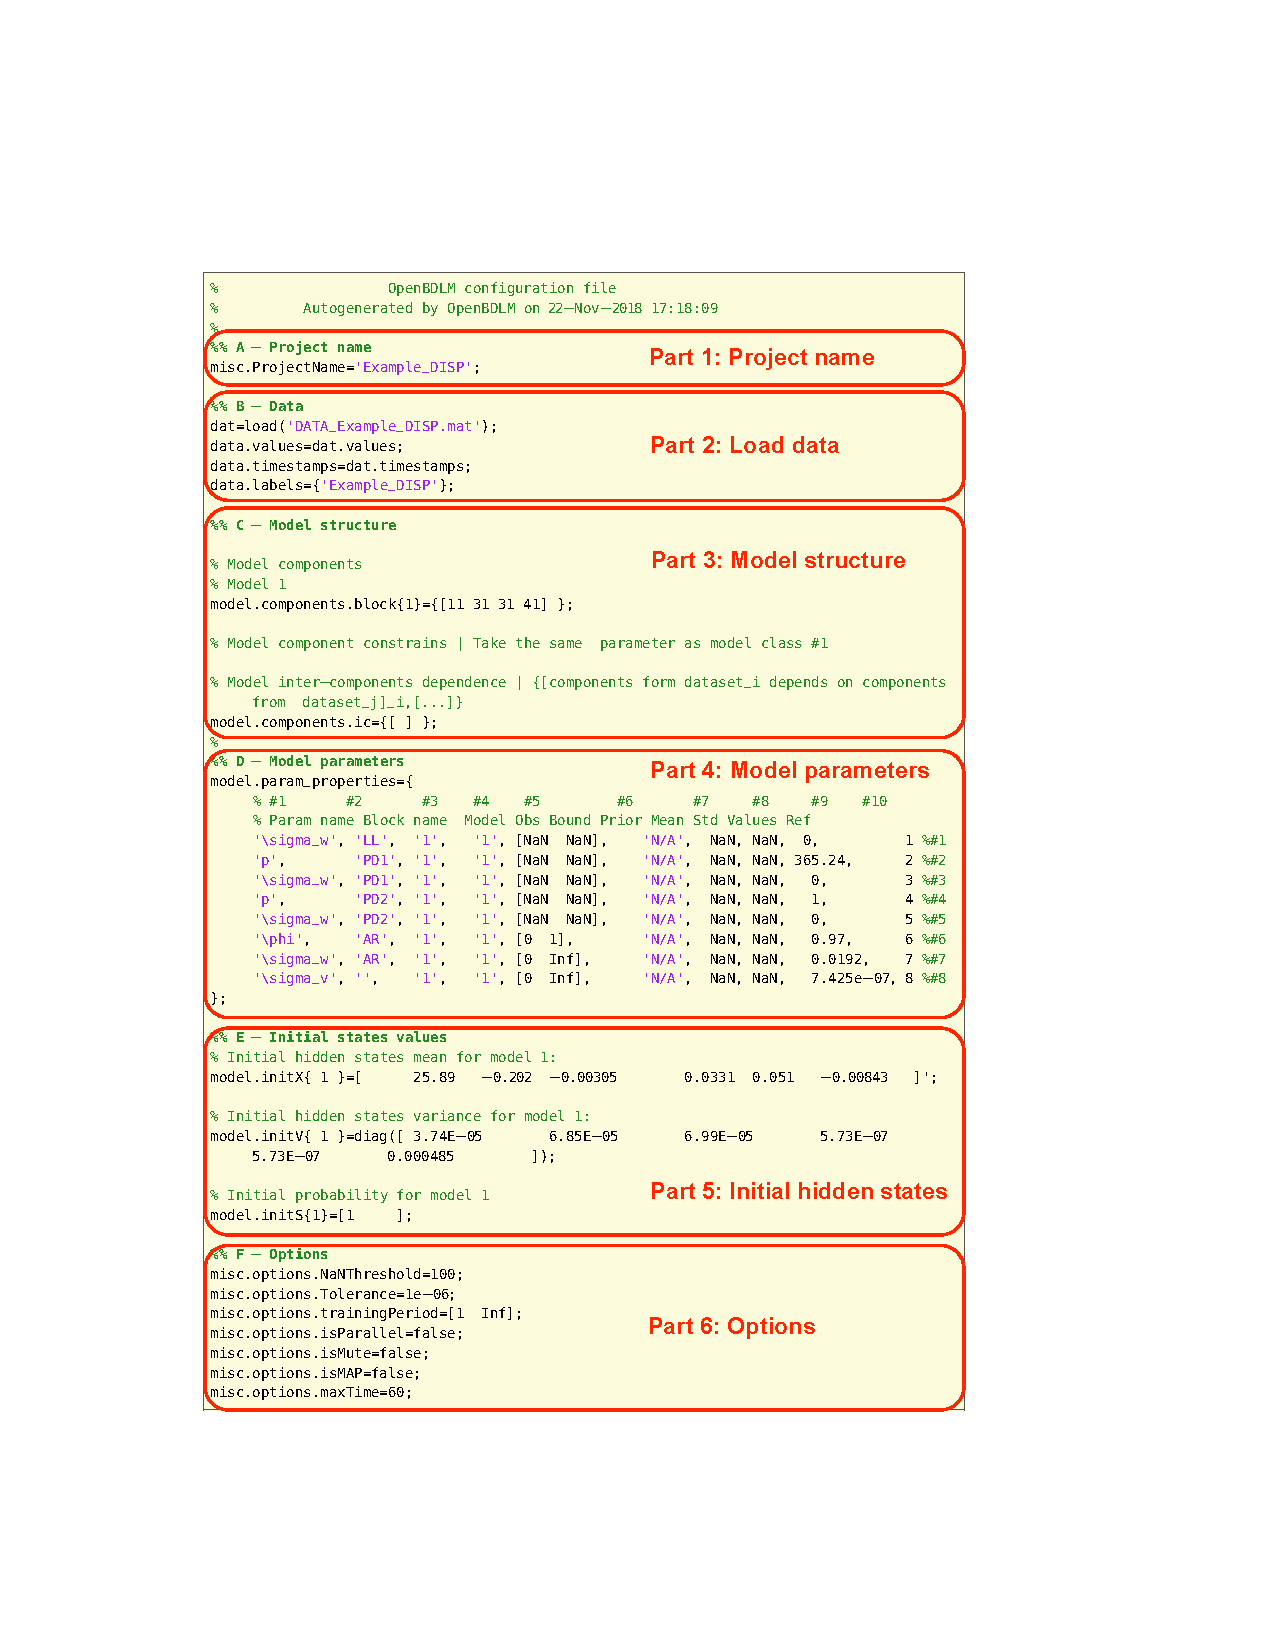
\includegraphics[width=115mm]{docfigs/Example_DISPSIM/listing/config_file_2.pdf}
\caption{Exemple of configuration file}
\label{fig:cfgfile}
\end{figure}

\subsection{Project name}
This section of the configuration file defines the name of the project as a vector of characters stored in the field \lstinline[basicstyle = \mlttfamily \small ]!ProjectName! of the \MATLAB{} variable \lstinline[basicstyle = \mlttfamily \small ]!misc!.

\subsection{Data}

This section of the configuration file defines information required for loading the data from a \lstinline[basicstyle = \mlttfamily \small ]!DATA_! file located in ``/data/mat'' subfolder.
The file must follow the format described in Section~\ref{SS:MATInput}.
The timestamp values, the amplitude values and the label values must be stored in the fields \lstinline[basicstyle = \mlttfamily \small]!timestamps!, \lstinline[basicstyle = \mlttfamily \small]!values!, and \lstinline[basicstyle = \mlttfamily \small]!labels! of the \MATLAB{} structure named \lstinline[basicstyle = \mlttfamily \small]!data!.

\subsection{Model structure}
\label{SS:ModelComponents}
This part of the configuration file defines the model in a \MATLAB{} structure named \lstinline[basicstyle = \mlttfamily \small]!model.component!.
The structure \lstinline[basicstyle = \mlttfamily \small]!model.component! must have three fields, named \lstinline[basicstyle = \mlttfamily \small]!model.component.block!, \lstinline[basicstyle = \mlttfamily \small]!model.component.ic!, and \lstinline[basicstyle = \mlttfamily \small]!model.component.const!.

\begin{itemize}

\item \lstinline[basicstyle = \mlttfamily \small ]!model.component.block!: it defines the block components associated with each time-series.
The field \lstinline[basicstyle = \mlttfamily \small ]!block! stores $1\times \mathtt{S}$ cell array, where $\mathtt{S} = \{1,2 \}$ is the number of model classes.
Each cell array is a $1\times \mathtt{D}$ cell array of matrice, where $\mathtt{D}$ is the number of time series.
Each block component is associated with a reference number:
\begin{itemize}
\item 11: Local level 
\item 12: Local trend
\item 13: Local acceleration
\item 21: Local level compatible with local trend
\item 22: Local level compatible with local acceleration
\item 23: Local trend compatible with local acceleration
\item 31: Periodic
\item 41: First-order autoregressive
\item 51: Kernel regression
\end{itemize}

\item  \lstinline[basicstyle = \mlttfamily \small ]!model.component.const!: it constrains model parameters between the block components from different model classes.
The field \lstinline[basicstyle = \mlttfamily \small ]!const! stores a $1\times \mathtt{S}$ cell array, where $\mathtt{S} = \{1, 2 \}$ is the total number of model classes.
It is defined only if $\mathtt{S} = 2$.
The first cell is empty, and the second cell is a $1\times \mathtt{D}$ cell array of array, where $\mathtt{D}$ is the number of time series.
The array contains $0$ and $1$ to indicate which block components of the second model class has the same model parameters than the corresponding component of the first model class. 
A value of $1$ indicates that the model parameters are constrained between the block components of the two model classes, $0$ otherwise.

\item  \lstinline[basicstyle = \mlttfamily \small ]!model.component.ic!:  it defines the dependencies among the time-series.
The field \lstinline[basicstyle = \mlttfamily \small ]!ic! stores a $1\times \mathtt{D}$ cell array of $1\times (\mathtt{D}-1)$ matrix, where $\mathtt{D}$ is the number of time series.
Each time series depend on the time series corresponding to the indexes given in the $\mathtt{D}$ arrays.
If the array is empty, the time-series are considered independent by default.

\end{itemize}


\subsection{Model parameters}
\label{SS:ModelParamProperties}
This part of the configuration file aims at defining the model parameters properties which are stored in the field named \lstinline[basicstyle = \mlttfamily \small ]!model.param_properties! of the \MATLAB{} structure \lstinline[basicstyle = \mlttfamily \small ]!model!.
The field \lstinline[basicstyle = \mlttfamily \small ]!model.param_properties! stores $\mathtt{K} \times 10$ cell array, where $\mathtt{K}$ is the total number of model parameters.
\begin{itemize}
\item column 1 must be a character vector that gives the name of the model parameters (e.g.  \lstinline[basicstyle = \mlttfamily \small ]!sigma_w!). 
\item column 2 must be a character vector that gives the reference name of the block associated with the parameter (e.g \lstinline[basicstyle = \mlttfamily \small ]!LL!, see Section~\ref{SS:BlockComponent}).
\item column 3 must be a character vector that gives the index corresponding to the model class associated with the parameter (e.g  either \lstinline[basicstyle = \mlttfamily \small ]!1! or \lstinline[basicstyle = \mlttfamily \small ]!2!) (see~\ref{SS:THSKF}).
\item column 4 must be a character vector that gives the index corresponding to the observation associated with the parameter (e.g \lstinline[basicstyle = \mlttfamily \small ]!3!).
\item column 5 must be a $1\times2$ array that gives the bound of the parameter (e.g \lstinline[basicstyle = \mlttfamily \small ]![NaN, NaN]!,  \lstinline[basicstyle = \mlttfamily \small ]![0, Inf]!, \lstinline[basicstyle = \mlttfamily \small ]![0, 1]!). 
The bounds are used to transform (if necessary) model parameters from a bounded to  an unbounded space during the optimization process (see Sections~\ref{S:PARAMESTIMATION} and~\ref{SS:THModelParameterEstimation}).
\item column 6 must be a character vector that gives the type of the prior used during the optimization process (e.g  either \lstinline[basicstyle = \mlttfamily \small ]!N/A! or \lstinline[basicstyle = \mlttfamily \small ]!normal!). 
\lstinline[basicstyle = \mlttfamily \small ]!N/A! indicates that no prior is used (see Sections~\ref{S:PARAMESTIMATION} and~\ref{SS:THModelParameterEstimation}).
\item column 7 must be a real number that gives the mean of the prior when a prior of type \lstinline[basicstyle = \mlttfamily \small ]!normal! is used, otherwise it must be set to \lstinline[basicstyle = \mlttfamily \small ]!NaN! (see Sections~\ref{S:PARAMESTIMATION} and~\ref{SS:THModelParameterEstimation}).
\item column 8 must be a real number that gives the standard deviation of the prior when a prior of type \lstinline[basicstyle = \mlttfamily \small ]!normal! is used, otherwise it must be set to \lstinline[basicstyle = \mlttfamily \small ]!NaN! (see Sections~\ref{S:PARAMESTIMATION} and~\ref{SS:THModelParameterEstimation}).
\item column 9 must be a real number that gives the value of the model parameters.
\item column 10 must be an integer that gives the reference number of the model parameters. The model parameters which share the same reference number are constrained to each other.
\end{itemize}

\subsection{Initial states values}
\label{SS:InitialHS}
This part of the configuration file defines the initial states values (at time $t=0$).
The initial mean and covariance hidden states values are stored in the \lstinline[basicstyle = \mlttfamily \small ]!model.initX! and \lstinline[basicstyle = \mlttfamily \small ]!model.initV! fields.
The initial probability for the model class is stored in the field \lstinline[basicstyle = \mlttfamily \small ]!model.initS!.

\begin{itemize}
\item \lstinline[basicstyle = \mlttfamily \small ]!model.initX!: $1\times \mathtt{S}$ cell array of array, where $\mathtt{S} = \{1, 2 \}$ is the total number of model classes.
Each array is $\mathtt{L}\times1$ array of real number that stores the initial mean values associated with each hidden states variables, where $\mathtt{L}$ is the total number of hidden states variables associated with the model.
\item \lstinline[basicstyle = \mlttfamily \small ]!model.initV!: $1\times \mathtt{S}$ cell array of array, where $\mathtt{S} = \{1, 2 \}$ is the total number of model classes.
Each array is $\mathtt{L}\times\mathtt{L}$ array of real number that stores the initial variance and covariances values associated with each hidden states variables.
\item \lstinline[basicstyle = \mlttfamily \small ]!model.initS!: $1\times \mathtt{S}$ cell array of array, where $\mathtt{S} = \{1, 2 \}$ is the total number of model classes. 
Each array is $1\times1$ array of real number that gives the initial probability for the model class.
\end{itemize}

\subsection{Options}
\label{SS:options}
This part of the configuration file defines the options that control different aspect of the software regarding the data pre-processing, optimization, hidden states estimation, and aspects related to graphical outputs.
The options are stored in the field named \text{options} of the \MATLAB{} variable \lstinline[basicstyle = \mlttfamily \small ]!misc!.
\begin{itemize}

\item Options for the data pre-processing

\begin{itemize}
\item \lstinline[basicstyle = \mlttfamily \small ]!misc.options.NaNThreshold!: real number that gives, in percent, the amount of missing data allowed at each time slice. Default: \lstinline[basicstyle = \mlttfamily \small ]!100!.
\item \lstinline[basicstyle = \mlttfamily \small ]!misc.options.Tolerance!: real number that gives the gives the duration (in number of days) after which two timestamps are not considered equal. Default: $10^{-6}$.

\end{itemize}


\item Options for the model parameters estimation

\begin{itemize}
\item \lstinline[basicstyle = \mlttfamily \small ]!misc.options.trainingPeriod!:  $1\times2$ array of real number that defines the training period, given in number of days since the first timestamp. Default: \lstinline[basicstyle = \mlttfamily \small ]![1 Inf]!. 
\item \lstinline[basicstyle = \mlttfamily \small ]!misc.options.isParallel!: logical that triggers or not the parallel computation for approximating the gradient in the optimization procedure. Note that parallel computation requires the \MATLAB{} \emph{Parallel Computing Toolbox}. Default: \lstinline[basicstyle = \mlttfamily \small ]!true!.
\item \lstinline[basicstyle = \mlttfamily \small ]!misc.options.maxIterations!: integer that gives the maximum number of iterations for the optimization procedure. Newton-Raphson only. Default: \lstinline[basicstyle = \mlttfamily \small ]!100!.
\item \lstinline[basicstyle = \mlttfamily \small ]!misc.options.maxTime!: real number that gives, in minutes, the maximum amount of  time to spend for the optimization procedure. Default: \lstinline[basicstyle = \mlttfamily \small ]!60!.
\item \lstinline[basicstyle = \mlttfamily \small ]!misc.options.isMAP!: logical that triggers or not the Maximum A Posteriori (MAP) estimation of the model parameters during the optimization procedure. MAP estimation includes prior information about the model parameters. Default: \lstinline[basicstyle = \mlttfamily \small ]!false!.
\item \lstinline[basicstyle = \mlttfamily \small ]!misc.options.isPredCap!: logical so that if \lstinline[basicstyle = \mlttfamily \small ]!isPredCap=true!, the Prediction Capacity (i.e. the log-likelihood over a test dataset) is used to drive the optimization process, otherwise the log-likelihood over the full dataset is used. This option is used only for Stochastic Gradient optimization. Default: \lstinline[basicstyle = \mlttfamily \small ]!false!.
\item \lstinline[basicstyle = \mlttfamily \small ]!misc.options.isLaplaceApprox!: logical so that if \lstinline[basicstyle = \mlttfamily \small ]!isLaplaceApprox=true! the posterior covariance matrix is estimated using Laplace approximation around the optimized model parameters values. This option is used only for Newton-Raphson optimization. Default: \lstinline[basicstyle = \mlttfamily \small ]!false!.
\item \lstinline[basicstyle = \mlttfamily \small ]!misc.options.NRTerminationTolerance!: real value determining the termination tolerance for the Newton-Raphson algorithm. Default: $10^{-7}$.
\item \lstinline[basicstyle = \mlttfamily \small ]!misc.options.NRLevelsLambdaRef!: integer that controls the number of trial loop for a parameter being optimized for theNewton-Raphson algorithm. Default: $4$.
\item \lstinline[basicstyle = \mlttfamily \small ]!misc.options.isMute!: logical so that if \lstinline[basicstyle = \mlttfamily \small ]!isMute=true!, no message are displayed on screen during the optimization procedure. Default: \lstinline[basicstyle = \mlttfamily \small ]!false!.
\item \lstinline[basicstyle = \mlttfamily \small ]!misc.options.maxEpochs!: integer that gives the maximum number of epochs the optimization procedure. This option is used only for Stochastic Gradient optimization. Default: \lstinline[basicstyle = \mlttfamily \small ]!50!.
\item \lstinline[basicstyle = \mlttfamily \small ]!misc.options.Optimizer!: vector of character that defines the optimizer for Stochastic Gradient algorithm. It must be either \lstinline[basicstyle = \mlttfamily \small ]!'MMT'!, \lstinline[basicstyle = \mlttfamily \small ]!'ADAM'!, \lstinline[basicstyle = \mlttfamily \small ]!'MMTbeta'!, \lstinline[basicstyle = \mlttfamily \small ]!'ADAMbeta'!. This option is used only for Stochastic Gradient optimization. Default: \lstinline[basicstyle = \mlttfamily \small ]!'MMT'!.
\item \lstinline[basicstyle = \mlttfamily \small ]!misc.options.SplitPercent!: real number that defines defines in percent the portion of the training data used for validation. Default: \lstinline[basicstyle = \mlttfamily \small ]!30!.
\item \lstinline[basicstyle = \mlttfamily \small ]!misc.options.MiniBatchSizePercent!: real number that defines defines the size of mini-batch, in percent of the training data. Default: \lstinline[basicstyle = \mlttfamily \small ]!20!.
\item \lstinline[basicstyle = \mlttfamily \small ]!misc.options.SGTerminationTolerance!: termination tolerance for the Stochastic gradient algorithm. This option is used only for Stochastic Gradient optimization. Default: \lstinline[basicstyle = \mlttfamily \small ]!0.95!.
\end{itemize}

\item Options for the estimation

\begin{itemize}
\item \lstinline[basicstyle = \mlttfamily \small ]!misc.options.MaxSizeEstimation!: real number that gives the maximum size, in Mb, for which the hidden states estimations are saved in the \lstinline[basicstyle = \mlttfamily \small ]!PROJ_! file at the end of the analysis. Default: \lstinline[basicstyle = \mlttfamily \small ]!100!.
\item \lstinline[basicstyle = \mlttfamily \small ]!misc.options.MethodStateEstimation!: vector of character. It must be either \lstinline[basicstyle = \mlttfamily \small ]!'kalman'! or \lstinline[basicstyle = \mlttfamily \small ]!'UD'!. it gives the method used for the estimation of the hidden states. Default: \lstinline[basicstyle = \mlttfamily \small ]!'kalman'!.
\item \lstinline[basicstyle = \mlttfamily \small ]!misc.options.DataPercent!: real number that gives in percent the amount of data, starting at $t=1$ used for the estimation of the initial hidden states. Default: \lstinline[basicstyle = \mlttfamily \small ]!100!.
\item \lstinline[basicstyle = \mlttfamily \small ]!misc.options.KRNumberControlPoints!: integer that gives the number of control points used for the periodic kernel regression component (see Section~\ref{SS:BlockComponent}). Default: \lstinline[basicstyle = \mlttfamily \small ]!100!.
\end{itemize}


\item Options for the synthetic data creation

\begin{itemize}
\item \lstinline[basicstyle = \mlttfamily \small ]!misc.options.Seed!: integer that controls the random number generation used to create synthetic data. Synthetic data created with the same seed are identical (useful to replicate results). If  \lstinline[basicstyle = \mlttfamily \small ]!misc.options.Seed=[]!, the seed is based on current time and therefore, a different sequence of random number  is generated at each run. Default: \lstinline[basicstyle = \mlttfamily \small ]!12345!.
\end{itemize}

\item Options for the graphical outputs

\begin{itemize}
\item \lstinline[basicstyle = \mlttfamily \small ]!misc.options.isPlotEstimations!: logical. if \lstinline[basicstyle = \mlttfamily \small ]!isPlotEstimations=true!, figures plotting the estimation results popup on screen each time the hidden states are estimated. Default: \lstinline[basicstyle = \mlttfamily \small ]!true!.
\item \lstinline[basicstyle = \mlttfamily \small ]!misc.options.FigurePosition!: $1\times4$ array of real number that gives the location and size of the drawable area, specified as a vector of the form [left bottom width height] in the current units of \MATLAB{}. Default: \lstinline[basicstyle = \mlttfamily \small ]![100, 100, 1300, 270]!
\item \lstinline[basicstyle = \mlttfamily \small ]!misc.options.isSecondaryPlot!: logical. if \lstinline[basicstyle = \mlttfamily \small ]!isSecondaryPlot=true!, a closeup over two weeks is plotted at the right of each figure. Default: \lstinline[basicstyle = \mlttfamily \small ]!false!.
\item \lstinline[basicstyle = \mlttfamily \small ]!misc.options.Subsample!: integer that controls the number of points that are displayed in the plots. The number of points to plot is divided by a factor given by the values of \lstinline[basicstyle = \mlttfamily \small ]!misc.options.Subsample!. Default: \lstinline[basicstyle = \mlttfamily \small ]!1!.
\item \lstinline[basicstyle = \mlttfamily \small ]!misc.options.Linewidth!: real number that controls the width of the line plotted in the figure. Default: \lstinline[basicstyle = \mlttfamily \small ]!1!.
\item \lstinline[basicstyle = \mlttfamily \small ]!misc.options.ndivx!: integer that controls the number of labels for abscissa x-axis in each figure. Default: \lstinline[basicstyle = \mlttfamily \small ]!4!.
\item \lstinline[basicstyle = \mlttfamily \small ]!misc.options.ndivy!: integer that controls the number of labels for ordinate y-axis in each figure. Default: \lstinline[basicstyle = \mlttfamily \small ]!3!.
\item \lstinline[basicstyle = \mlttfamily \small ]!misc.options.Xaxis_lag!: real number that gives in number of days the amount of time by which the x-axis is shifted on each figure. Default: \lstinline[basicstyle = \mlttfamily \small ]!0!. 
\item \lstinline[basicstyle = \mlttfamily \small ]!misc.options.isExportTEX!: logical so that if \lstinline[basicstyle = \mlttfamily \small ]!isExportTEX=true!, figures are exported in \LaTeX{} format. Default: \lstinline[basicstyle = \mlttfamily \small ]!false!.
\item \lstinline[basicstyle = \mlttfamily \small ]!misc.options.isExportPNG!: logical so that if \lstinline[basicstyle = \mlttfamily \small ]!isExportPNG=true!,  figures are exported in PNG format. Default: \lstinline[basicstyle = \mlttfamily \small ]!false!.
\item \lstinline[basicstyle = \mlttfamily \small ]!misc.options.isExportPDF!: logical so that if \lstinline[basicstyle = \mlttfamily \small ]!isExportPDF=true!,  figures are exported in PDF format. Default: \lstinline[basicstyle = \mlttfamily \small ]!false!.
\end{itemize}
\end{itemize}

\section{Workflow}
\label{S:WORKFLOW}

\begin{figure}[h]
  \centering
\scalebox{0.7}{
\!\!\!\!\!\!\!\!\begin{tikzpicture}

% Node position
\node[paraamber](rawdata){\begin{tabular}{c}  .MAT \\ and \\ .CSV data files \end{tabular}};
\node[esamber, below of=rawdata, yshift=-1.3cm] (preprocess) {\begin{tabular}{c}  pre- \\   processing \end{tabular} };
\node[test, below of=preprocess,  yshift=-1.3cm] (testpreprocess) {? };
\node[esbisque, right of=testpreprocess, xshift = 1.75cm ] (configmodel) {  \begin{tabular}{c}  model \\  configuration \end{tabular} };
\node[esbisque, right of=configmodel, xshift = 1.75cm ] (buildmodel) {   \phantom{} build model \phantom{} };
\node[esbabyblueeyes, right of=buildmodel, xshift=1.75cm] (paramlearning){\begin{tabular}{c}   parameters \\  learning \end{tabular}};
\node[parawhite, below of=paramlearning, xshift=0cm, yshift = -1.5cm] (inputcfg){\begin{tabular}{c}  CFG\_*.m \\  DATA\_*.mat \end{tabular}};
\node[test, right of=paramlearning, xshift = 1.5cm] (testparamlearning) {?};
\node[esceladon, right of=testparamlearning, xshift = 1.5cm] (stateestimation) {\begin{tabular}{c}   states \\   estimation \end{tabular}};
\node[test, right of=stateestimation, xshift = 1.5cm] (teststateestimation) {?};
\node[parawhite, right of=teststateestimation, xshift = 2.25cm] (results) {\begin{tabular}{c}  CFG\_*.m  \\  DATA\_*.mat \\ RES\_*.mat \\ PROJ\_*.mat \\  LOG\_*.txt  \end{tabular}};
\node[user, below of=testpreprocess, yshift=-2.5cm] (user1) { 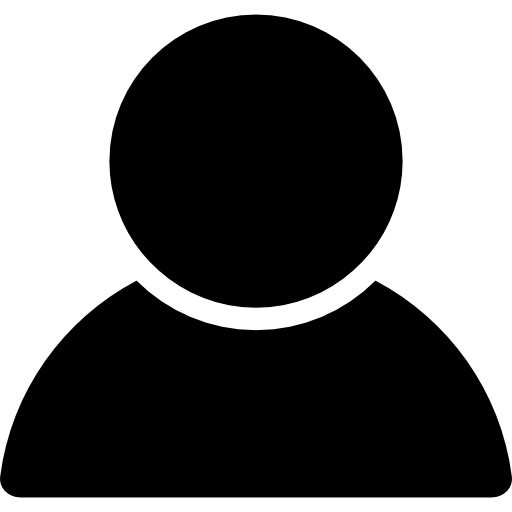
\includegraphics[height=0.45cm]{./docfigs/user_logo.png}};
\node[user, below of=configmodel, yshift=-2.5cm] (user2) { 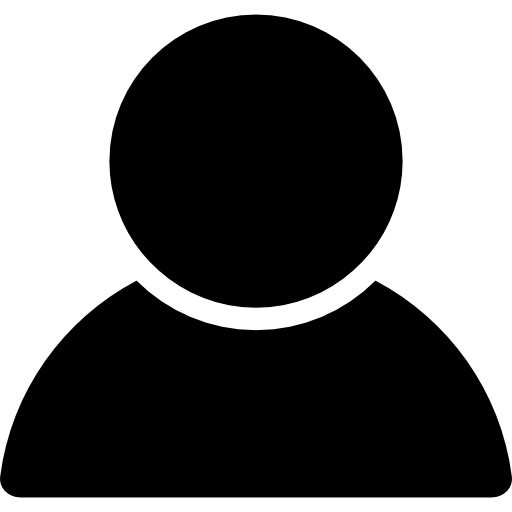
\includegraphics[height=0.45cm]{./docfigs/user_logo.png}};
\node[user, below of=testparamlearning, yshift=-2.5cm] (user3) { 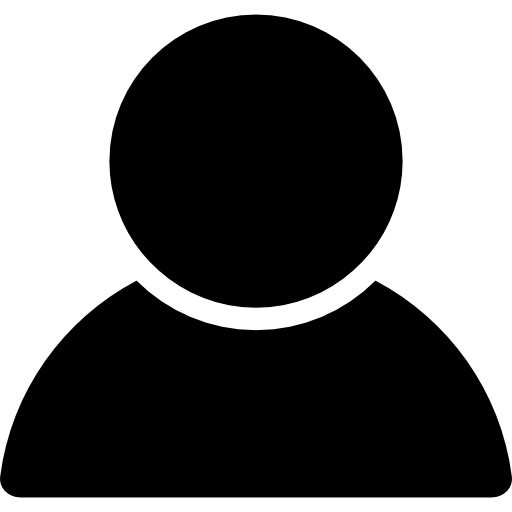
\includegraphics[height=0.45cm]{./docfigs/user_logo.png}};
\node[user, below of=teststateestimation, yshift=-2.5cm] (user4) { 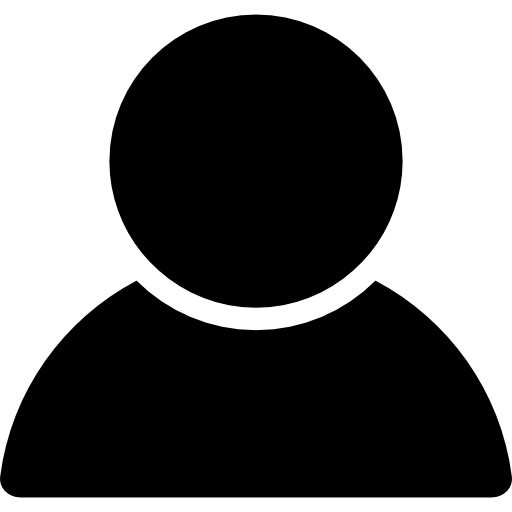
\includegraphics[height=0.45cm]{./docfigs/user_logo.png}};
\node[eslightgray, above of=paramlearning, yshift=4cm, xshift=0cm](syntheticdatacreation) {\phantom{} synthetic data creation \phantom{}};

 % Define path
\path[->, thick]  (rawdata)edge(preprocess);
\path[-, thick]  (preprocess)edge(testpreprocess);
\path[<->, thick]  (testpreprocess)edge(user1);
\path[-, thick]  (configmodel)edge(buildmodel);
\path[<->, thick]  (configmodel)edge(user2);
\path[-, thick]  (buildmodel)edge(paramlearning);
\path[-, thick]  (paramlearning)edge(testparamlearning);
\path[<->, thick]  (testparamlearning)edge(user3);
\path[-, thick]  (testparamlearning)edge(stateestimation);
\path[-, thick] (stateestimation) edge (teststateestimation);
\path[<->, thick]  (teststateestimation)edge(user4);
\path[-, thick] (testpreprocess) edge node[anchor=center, above] { yes}  (configmodel);
\path[->, draw, thick] (testpreprocess.west) -| (-1.25cm,-3cm) |- node[anchor=center, above, rotate=90, fill=none]{ no} (preprocess.west);
\path[->, thick] (teststateestimation) edge node[anchor=center, above] { yes}  (results);
\path[->, draw, thick] (testparamlearning.north) |- (9cm,-2.5cm) -| node[anchor=center, above, rotate=0, fill=none]{ no} (paramlearning.north);
\path[-, draw, thick] (testparamlearning)  edge node[anchor=center, above] { yes}  (stateestimation);
\path[->, draw, thick] (teststateestimation.north) |- (6cm,-2cm) -| node[anchor=center, above, rotate=0, fill=none]{ no} (buildmodel.north);
\path[->, draw, thick] (inputcfg) edge (paramlearning);

\path[->, draw, thick, dashed] (buildmodel.east) -| (6.75cm, -0.75cm) -| (syntheticdatacreation.south);
\path[->, draw, thick, dashed] (paramlearning.east) -| (9.75cm, -0.75cm) -| (syntheticdatacreation.south);
\path[->, draw, thick, dashed] (stateestimation.east) -| (14.5cm, -0.75cm) -| (syntheticdatacreation.south);
\path[->, draw, thick, dashed] (syntheticdatacreation.north) |- (9cm, 2cm) -| (rawdata.north);
\path[->, draw, thick, dashed] (syntheticdatacreation.north) |- (18cm, 2cm) -| (results.north);

 % Rectangle
\draw [draw=amber, line width=0.5mm, dashed ] (-3cm, -3cm) rectangle ++(5cm , 4cm );
\draw [draw=bisque, line width=0.5mm, dashed ] (0.95cm,-5.55cm) rectangle ++(5.85cm , 2cm );
\draw [draw=babyblueeyes, line width=0.5mm, dashed ] (7cm,-5.55cm) rectangle ++(2.5cm , 2cm );
\draw [draw=celadon, line width=0.5mm, dashed ] (11.85cm,-5.55cm) rectangle ++(2.75cm , 2cm );
\draw [draw=lightgray, line width=0.5mm, dashed ] (6cm,-0.5cm) rectangle ++(4.5cm , 1.75cm );
 
 % Text
\node[ above of = rawdata, xshift = -0.5cm, yshift = 0.325 cm, fill=white] { Section~\ref{S:DATALOADING} and~\ref{S:DATAEDITINGPREPROCESSING}};
\node[ above of = buildmodel, xshift = -1cm, yshift = 0.325 cm, fill=white] { Section~\ref{S:MODELCONFIGURATION} and~\ref{S:MODELCONSTRUCTION}};
\node[above of = paramlearning, xshift = 0cm, yshift = 0.325 cm,  fill=white] { Section~\ref{S:PARAMESTIMATION} };
\node[above of = stateestimation, xshift = 0cm, yshift = 0.325 cm,  fill=white] { Section~\ref{S:HIDDENSTATESESTIMATION} };
\node[above of = syntheticdatacreation, xshift = 0cm, yshift = 0.325 cm,  fill=white] { Section~\ref{S:SYNTHETIC}};

\end{tikzpicture} }
\label{FIG:OpenBDLMworkflow}
\caption{OpenBDLM workflow}
\end{figure}

\subsection{Data loading}
\label{S:DATALOADING}
\subsubsection{Input data format}

OpenBDLM supports two types of input data format.

% depending whether the time series are synchronous, or not.
%The time series are synchronous if they all share the same time vector. % and have the same number of data points.
%Conversely, time series are asynchronous if they do not all share the same time vector.
%\subsubsection{Input data formatting for asynchronous time series}

\paragraph{Comma Separated Values files (.CSV)}
\label{SS:CSVInput}

%Comma Separated Values (CSV) data formatting is generally used to load time series data, which have not been synchronized yet.
%If the data have already been synchronized, it is preferable to use properly formatted .MAT \MATLAB{} files (see Section~\ref{SS:MatFiles})
One .CSV data file must be provided for each time series.
The file must contain two columns that are organized as shown in Listing~\ref{LST:CSV_Formatting}.
\begin{lstlisting}[ frame = single, linewidth = \linewidth, caption = CSV data file example,  label = LST:CSV_Formatting, float = ht, ,captionpos=b]
'name'            ,   '2000-01-01-22-00-00'
737422            ,   0.40
737423.5          ,   0.21
737424            ,   0.548
7374245.25        ,   NaN
7374246           ,   0.57
\end{lstlisting}    
The first line of the file is the header.
In the header, the first field must contain the label of the time series given as a quoted delimited string, as \textquotesingle name\textquotesingle .
The second field is the date of the first timestamp given as a quoted delimited string, formatted as \textquotesingle YYYY-DD-MM-HH-MM-SS\textquotesingle.  
For the remaining lines, the first field is the date given as a serial date number in number of days, given as a real number, and the second field is the magnitude of the physical quantity measured, given as a real number.
The missing data must be indicated as \lstinline[basicstyle = \mlttfamily \small ]!NaN! number.
The .csv files must be stored in the ``OpenBDLM-master/data/csv'' subfolder.

\paragraph{\MATLAB{} files (.MAT)}
\label{SS:MATInput}

The \MATLAB{} binary .MAT file must contain three \MATLAB{} variables called \lstinline[basicstyle = \mlttfamily \small]!labels!, \lstinline[basicstyle = \mlttfamily \small]!timestamps!, and \lstinline[basicstyle = \mlttfamily \small]!values!.
\begin{itemize}
\item \lstinline[basicstyle = \mlttfamily \small]!labels!: $1\times \mathtt{D}$ cell array containing the reference name associated with each time series, where $\mathtt{D}$ is the number of time series.
\item \lstinline[basicstyle = \mlttfamily \small]!timestamps!: $\mathtt{N}\times 1$ array containing the timestamps given as serial date number from January 0, 0000, where $\mathtt{N}$ is the number of data samples.
\item \lstinline[basicstyle = \mlttfamily \small]!values!: $\mathtt{N}\times \mathtt{D}$ array containing the data amplitude values.
\end{itemize}
 \MATLAB{} binary .mat files must be stored in the ``OpenBDLM-master/data/mat'' subfolder.
Note that \MATLAB{} binary .MAT files can be used to load at once several time series which share the same timestep vector (i.e. synchronous time series, see Section~\ref{S:DATAEDITINGPREPROCESSING}  for details.)


\subsubsection{Data loading functions}

The data loading workflow is presented Figure~\ref{FIG:DataLoadingWorkflow}. The list of OpenBDLM functions used for data loading is:

\begin{description}[style=unboxed]
\item[Control script to load data] \leavevmode
  \begin{lstlisting}[ basicstyle = \mlttfamily \small, breaklines=true]
[data,misc,dataFilename]=DataLoader(misc)
 \end{lstlisting}

\item[Loads data] \leavevmode
  \begin{lstlisting}[ basicstyle = \mlttfamily \small, breaklines=true]
[dataOrig,misc]=loadData(misc)
 \end{lstlisting}

\item[Reads data from multiple data files]  \leavevmode
  \begin{lstlisting}[ basicstyle = \mlttfamily \small, breaklines=true]
[dataOrig,misc]=readMultipleDataFiles(misc)
 \end{lstlisting}

 \item[Reads a single CSV file]  \leavevmode
  \begin{lstlisting}[ basicstyle = \mlttfamily \small, breaklines=true]
[dat,label]=readSingleCSVFile(FileToRead,varargin)
 \end{lstlisting}
 
  \item[Reads a single MAT file]  \leavevmode
  \begin{lstlisting}[ basicstyle = \mlttfamily \small, breaklines=true]
[dat,label]=readSingleMATFile(FileToRead,varargin)
 \end{lstlisting}
 
   \item[Saves data in a DATA\_  \MATLAB{} MAT file]  \leavevmode
  \begin{lstlisting}[ basicstyle = \mlttfamily \small, breaklines=true]
[misc,dataFilename]= saveDataBinary(data,misc,varargin)
 \end{lstlisting}
 
    \item[Saves data in separate CSV files]  \leavevmode
  \begin{lstlisting}[ basicstyle = \mlttfamily \small, breaklines=true]
[misc]= saveDataCSV(data,misc,varargin)
 \end{lstlisting}
 
\end{description}


\begin{figure}[!h]
  \centering
  \captionsetup{justification=centering}
\scalebox{0.8}{
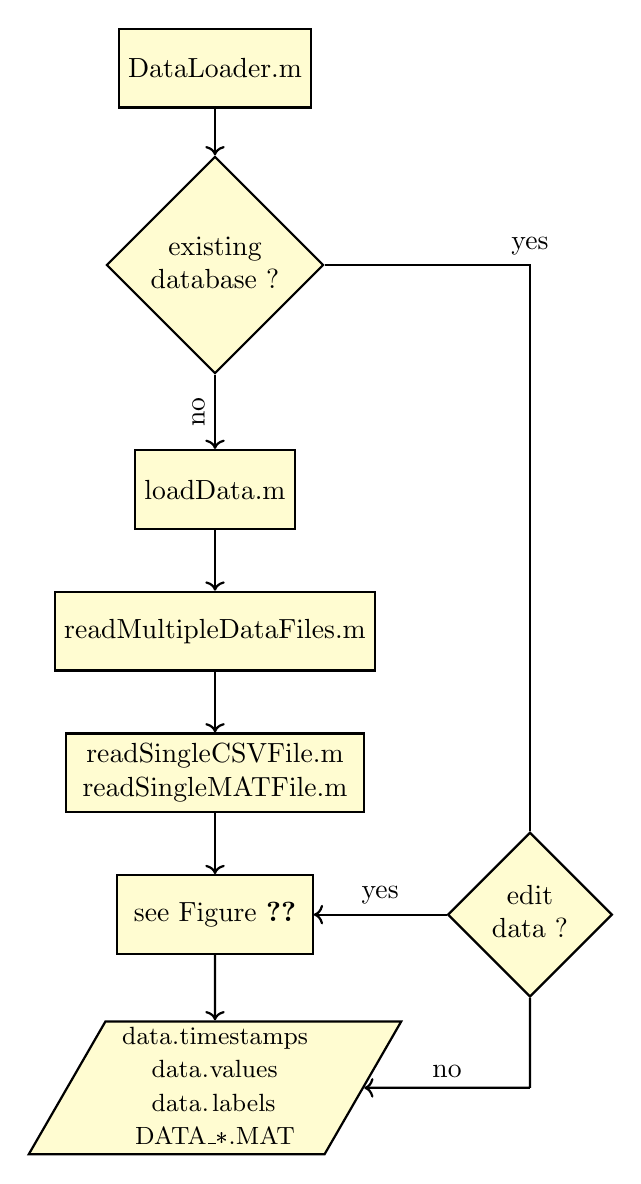
\begin{tikzpicture}


%\node[paraamber](inputDataLoader){\lstinline[basicstyle = \mlttfamily \small ]!data!};
\node[esamber](DataLoader){ \phantom{} DataLoader.m \phantom{} };
\node[testamber](testExistDatabase)[below of = DataLoader, yshift = -1.5cm]{\begin{tabular}{c} existing \\ database  ? \end{tabular}};
\node[esamber](loadData)[below of = testExistDatabase, yshift=-1.85cm, xshift = 0cm]{ \phantom{} loadData.m \phantom{} };
\node[esamber](readMultipleDataFiles)[below of = loadData, xshift = 0cm, yshift=-0.8cm, ]{ \phantom{} readMultipleDataFiles.m \phantom{} };
\node[esamber](readSingleFile)[below of = readMultipleDataFiles, yshift= -0.8cm]{\begin{tabular}{c} readSingleCSVFile.m \\ readSingleMATFile.m  \end{tabular}};
\node[esamber](editData)[below of = readSingleFile, yshift= -0.8cm]{\begin{tabular}{c}  see Figure~\ref{FIG:DataEditingWorkflow} \end{tabular}};

\node[testamber](testEditData)[right of = editData, yshift= 0cm, xshift=3cm ]{\begin{tabular}{c} edit \\ data ?  \end{tabular}};

\node[paraamber](DataMATFile)[below of =editData, yshift=-1.2cm, xshift = 0cm]{\begin{tabular}{c} \lstinline[basicstyle = \mlttfamily \small ]!data.timestamps! \\ \lstinline[basicstyle = \mlttfamily \small ]!data.values! \\ \lstinline[basicstyle = \mlttfamily \small ]!data.labels! \\ \lstinline[basicstyle = \mlttfamily \small ]!DATA_*.MAT!  \end{tabular}};
%\path[->, thick] (inputDataLoader)edge(DataLoader);
\path[->, thick] (DataLoader)edge(testExistDatabase);
\path[->, thick] (testExistDatabase)edge node[anchor=center, above, rotate=0, rotate=90]{ no}  (loadData);
\path[->, thick] (loadData)edge(readMultipleDataFiles);
\path[->, thick] (readMultipleDataFiles)edge(readSingleFile);
\path[->, thick] (readSingleFile)edge (editData);
\path[->, thick] (editData)edge (DataMATFile);
\path[<-, thick] (editData)edge node[anchor=center, above, rotate=0]{ yes}  (testEditData);
\path[-, draw, thick] (testExistDatabase.east) -| (3cm,-2.5cm) -| node[anchor=center, above, rotate=0]{ yes} (testEditData.north);
\path[->, draw,  thick] (testEditData.south) |- (4cm, -12.95cm) -- node[anchor=center, above, rotate=0]{no} (DataMATFile.east);

\end{tikzpicture} } 
\caption{Data loading workflow} \label{FIG:DataLoadingWorkflow}
\end{figure}

\subsection{Data pre-processing}
\label{S:DATAEDITINGPREPROCESSING}

Data pre-processing is a step taken ahead of data analysis.
In most cases, the set of available time series is heterogeneous, in the sense that each time series does not originate from the same system of acquisition.
Therefore, the raw data do not usually share the same time vectors.
This is an issue because BDLM is not capable to analyze asynchronous time series.
Therefore, the main objective of data pre-processing is to synchronize the time series. 
Moreover, data pre-processing includes time series selection, data analysis time period selection, \lstinline[basicstyle = \mlttfamily \small ]!NaN! removal, and data resampling.
%The time synchronization is performed automatically through the data editing process.

\begin{lstlisting}[ frame = single, basicstyle = \mlttfamily \small,  linewidth = \linewidth, caption = OpenBDLM data editing menu,  label = LST:Editing_menu, float = h!, ,captionpos=b]
- Data editing and preprocessing. Choose from:

     1  ->  Select time series
     2  ->  Select data analysis time period 
     3  ->  Remove missing data
     4  ->  Resample
     5  ->  Change synchronization options

     6  ->  Reset changes
     7  ->  Save changes and continue analysis

     choice >> 
\end{lstlisting}    

\subsubsection{Selection of time series}
\label{SS:SelectionTimeSeries}

The selection of time series allows including a subset of the time series. Note that time series are automatically synchronized as they are added to (or removed from) the dataset.

\subsubsection{Selection of data analysis time-window}
\label{SS:SelectionPeriodAnalysis}

The selection of the analysis time-window allows selecting a portion of data between two dates.
The date format follows \textquotesingle YYYY-DD-MM\textquotesingle {}.
If the second requested date exceeds the date associated with the last data sample of the original dataset, padding with \lstinline[basicstyle = \mlttfamily \small ]!NaN! values is performed. 
The timestep for the padding must be provided by the user.

\subsubsection{Removing missing data}
\label{SS:MissingDataRemoval}

It is possible to control the maximum amount of missing data (\lstinline[basicstyle = \mlttfamily \small ]!NaN!) allowed at each time slice. 
The maximum amount of \lstinline[basicstyle = \mlttfamily \small ]!NaN! allowed at each time slice is given in percent with respect to the total number of time series.
By default, the maximum amount of missing data is 100\% (see variable \lstinline[basicstyle = \mlttfamily \small ]!misc.options.NaNThreshold!).

\subsubsection{Data resampling}
\label{SS:DataResampling}
Data resampling changes the sampling rate of the time series according to a given timestep provided by the user. 
If the requested timestep is higher than the original data timestep, \lstinline[basicstyle = \mlttfamily \small ]!NaN! values are added.
Conversely, if the requested timestep is lower than the original  data timestep, OpenBDLM averages the data amplitude values within non-overlapping fixed time windows, each having the duration of the requested timestep.
The first time window starts at the first timestamp, and the new timestamps are assigned at the times corresponding to the mid point of each time window.

\subsubsection{Time synchronization options}
\label{SS:synchronization}
By default, the time synchronization in OpenBDLM is done by padding with \lstinline[basicstyle = \mlttfamily \small ]!NaN! values.
The time synchronization is controlled by the \lstinline[basicstyle = \mlttfamily \small ]!NaNThreshold! and \lstinline[basicstyle = \mlttfamily \small ]!tolerance! variables.
\lstinline[basicstyle = \mlttfamily \small ]!NaNThreshold!  is given in percent with respect to the total number of time series.
The variable \lstinline[basicstyle = \mlttfamily \small ]!tolerance! gives the duration (in number of days) after which two timestamps are not considered equal.
The default values for \lstinline[basicstyle = \mlttfamily \small ]!NaNThreshold!  and \lstinline[basicstyle = \mlttfamily \small ]!tolerance! are 100\% and $10^{-6}$ days, respectively (see variables \lstinline[basicstyle = \mlttfamily \small ]!misc.options.NaNThreshold! and \lstinline[basicstyle = \mlttfamily \small ]!misc.options.tolerance!. % $100$\% and $10^{-6}$ days, respectively. 

\subsubsection{Data pre-processing functions}

The data pre-processing workflow is presented Figure~\ref{FIG:DataEditingWorkflow}. The list of OpenBDLM functions used for data editing is:

\begin{description}[style=unboxed]
\item[Control script to pre-process the dataset (selection, resampling, etc..)] \leavevmode
  \begin{lstlisting}[ basicstyle = \mlttfamily \small, breaklines=true]
[data,misc,dataFilename]=editData(data,misc,varargin)
 \end{lstlisting}

\item[Requests the user to select some time series] \leavevmode
  \begin{lstlisting}[ basicstyle = \mlttfamily \small, breaklines=true]
[data,misc]=chooseTimeSeries(data,misc)
 \end{lstlisting} 
 
\item[Creates a single time vector from a set of time series] \leavevmode
  \begin{lstlisting}[ basicstyle = \mlttfamily \small, breaklines=true]
[data,misc]=mergeTimeStampVectors(dataOrig,misc,varargin)
 \end{lstlisting} 
 
\item[Resamples dataset according to a given timestep] \leavevmode
  \begin{lstlisting}[ basicstyle = \mlttfamily \small, breaklines=true]
[data_resample,misc]=resampleData(data,misc,varargin)
 \end{lstlisting} 
 
 \item[Selects data between two dates] \leavevmode
  \begin{lstlisting}[ basicstyle = \mlttfamily \small, breaklines=true]
[data,misc]=selectTimePeriod(data,misc)
 \end{lstlisting} 
 
  \item[Computes the timestep vector from the timestamps vector] \leavevmode
  \begin{lstlisting}[ basicstyle = \mlttfamily \small, breaklines=true]
[timesteps]=computeTimeSteps(timestamps)
 \end{lstlisting} 
 
   \item[Display information about stored data on screen] \leavevmode
  \begin{lstlisting}[ basicstyle = \mlttfamily \small, breaklines=true]
displayData(data,misc)
 \end{lstlisting} 
 
    \item[ Display the list of DATA\_*.mat files ] \leavevmode
  \begin{lstlisting}[ basicstyle = \mlttfamily \small, breaklines=true]
[FileInfo]= displayDataBinary(misc,varargin)
 \end{lstlisting} 
 
\end{description}

\begin{figure}[!h]
  \centering
  \captionsetup{justification=centering}
\scalebox{0.8}{
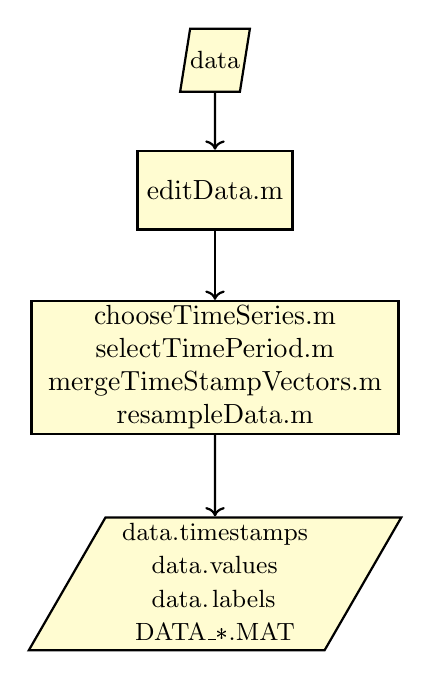
\begin{tikzpicture}

\node[paraamber](inputDataEditor){\lstinline[basicstyle = \mlttfamily \small ]!data!};
\node[esamber](editData)[below of = inputDataEditor,  yshift=-0.65cm, xshift = 0cm ]{ \phantom{} editData.m \phantom{} } ;
\node[esamber](editFunctions)[below of = editData, yshift = -1.25cm]{\begin{tabular}{c} chooseTimeSeries.m \\ selectTimePeriod.m \\ mergeTimeStampVectors.m \\ resampleData.m \end{tabular}};
\node[paraamber](DataMATFile)[below of =editFunctions, yshift=-1.75cm, xshift = 0cm]{\begin{tabular}{c} \lstinline[basicstyle = \mlttfamily \small ]!data.timestamps! \\ \lstinline[basicstyle = \mlttfamily \small ]!data.values! \\ \lstinline[basicstyle = \mlttfamily \small ]!data.labels! \\ \lstinline[basicstyle = \mlttfamily \small ]!DATA_*.MAT!  \end{tabular}};

\path[->, thick] (inputDataEditor)edge(editData);
\path[->, thick] (editData)edge(editFunctions);
\path[->, thick] (editFunctions)edge(DataMATFile);

\end{tikzpicture} } 
\caption{Data pre-processing workflow} \label{FIG:DataEditingWorkflow}
\end{figure}



\subsection{Model configuration}
\label{S:MODELCONFIGURATION}
%After loading and pre-processing the data, the next step of the analysis is the model configuration.
Model configuration includes, (i) defining the number of model class, (ii) defining the dependencies between the time series in case of multiple time series analysis, (iii) defining the block components which are assigned to each time series and model class, (iv) defining possible constrain between model parameters.
%The dependencies between time series as well as constrains between model parameters of different model class are also handled during the configuration of the model.
The \MATLAB{} structure named \lstinline[basicstyle = \mlttfamily]!model.component! stores all the information about the model configuration.
The structure \lstinline[basicstyle = \mlttfamily]!model.component! has three fields named  \lstinline[basicstyle = \mlttfamily]!model.component.ic!, \lstinline[basicstyle = \mlttfamily]!model.component.block!, and \lstinline[basicstyle = \mlttfamily]!model.component.const!.

\subsubsection{Dependencies between time series}

The field \lstinline[basicstyle = \mlttfamily]!model.component.ic! stores the information related to time series dependencies.
\lstinline[basicstyle = \mlttfamily \small ]!model.component.ic! stores a $1\times \mathtt{D}$ cell array of $(1\times \mathtt{D}-1)$ matrix, where $\mathtt{D}$ is the number of time series.
Each time series depend on the time series corresponding to the indexes given in the $\mathtt{D}$ arrays.
If the array is empty, the time series are independent. See the Reference Theory \S\ref{S:Dependencies} for further details.

\subsubsection{Block components}

OpenBDLM supports 5 types of block components: (1) baseline, (2) periodic, (3) periodic kernel regression, (4) autoregressive, and (5) level intervention. 
(1) The baseline component models the local mean of the time series. 
There are three types of baseline supported in OpenBDLM: (i) level model, (ii) trend model, (iii) acceleration model. 
(2) The periodic component models harmonic periodic phenomena. %, which are most often related to external effects.
(3) The periodic kernel regression models non-harmonic periodic pattern.
(4) The autoregressive component is intended as a residual term to capture the time-dependent model errors.
(5) The level intervention component allows estimating the magnitude of discrete jumps occurring in the local level at specific timestamps provided by the user.
The field \lstinline[basicstyle = \mlttfamily \small ]!block! stores a $1\times \mathtt{S}$ cell array, where $\mathtt{S} \in \{1,2 \}$ is the number of model classes.
Each cell array is a $1\times \mathtt{D}$ cell array of array, where $\mathtt{D}$ is the number of time series.
Each block component is associated with a reference number:
\begin{itemize}\setlength\itemsep{0em}
\item 11: Local level 
\item 12: Local trend
\item 13: Local acceleration
\item 21: Local level compatible with local trend
\item 22: Local level compatible with local acceleration
\item 23: Local trend compatible with local acceleration
\item 31: Periodic
\item 41: First-order autoregressive
\item 51: Kernel regression
\item 61: Level intervention
\end{itemize}
The number of hidden states associated with each block component can be different. 
Each block component can be replicated, each having its own set of model parameters. 
For instance, two periodic components with periods of 365 days and 1 day can be used to model seasonal and daily variations, respectively. See the Reference Theory \S\ref{SS:BlockComponent} for further details.

\subsubsection{Parameter constrains}

The variable \lstinline[basicstyle = \mlttfamily]!model.component.const! stores a $1\times \mathtt{S}$ cell array, where $\mathtt{S} \in \{1, 2 \}$ is the total number of model classes.
It is defined only if $\mathtt{S} = 2$.
The first cell is empty, and the second cell is a $1\times \mathtt{D}$ cell array of array, where $\mathtt{D}$ is the number of time series.
The array contains $0$ and $1$ to indicate which block components of the second model class has the same model parameters than the corresponding component of the first model class. 
A value of $1$ indicates that the model parameters are constrained between the block components of the two model classes, $0$ otherwise.

\subsubsection{Number of model class}

OpenBDLM is capable of detecting regime changes in the dynamics in the baseline of the time series. Therefore, OpenBDLM handles model switching between the three types of baseline dynamics, that is, local level, local trend, and local acceleration models. OpenBDLM supports a maximum of two model dynamics, which includes six types of model switch: (1) from local level model to local trend model (and reverse), (2) from local level model to acceleration model (and reverse), (3) from local trend to acceleration model (and reverse).


\subsubsection{Model configuration functions}

The model configuration workflow is presented Figure~\ref{FIG:ModelConfigurationWorkflow}. The list of OpenBDLM functions used for model configuration is:

\begin{description}[style=unboxed]\setlength\itemsep{0em}
\item[Controls script for model configuration ] \leavevmode
  \begin{lstlisting}[ basicstyle = \mlttfamily \small, breaklines=true]
[data,model,estimation,misc]=ModelConfiguration(data,model,estimation,misc)
 \end{lstlisting}
 
 \item[Model configuration for real data ] \leavevmode
  \begin{lstlisting}[ basicstyle = \mlttfamily \small, breaklines=true]
[data,model,estimation,misc]=configureModelForDataReal(data,model,estimation,misc)
 \end{lstlisting}
 
  \item[Model configuration for synthetic data (for synthetic data creation only)] \leavevmode
  \begin{lstlisting}[ basicstyle = \mlttfamily \small, breaklines=true]
[data,model,estimation,misc]=configureModelForDataSimulation(data,model,estimation,misc)
 \end{lstlisting}
 
   \item[Requests user's input to configure the model] \leavevmode
  \begin{lstlisting}[ basicstyle = \mlttfamily \small, breaklines=true]
[model,misc]=defineModel(data,misc)
 \end{lstlisting}
 
    \item[Requests user's input to define time series labels/reference name (for synthetic data creation only)] \leavevmode
  \begin{lstlisting}[ basicstyle = \mlttfamily \small, breaklines=true]
  [data,misc]=defineDataLabels(data,misc)
 \end{lstlisting}
 
     \item[Requests user's input to define data timestamps (for synthetic data creation only)] \leavevmode
  \begin{lstlisting}[ basicstyle = \mlttfamily \small, breaklines=true]
[data,misc]=defineTimestamps(data,misc)
 \end{lstlisting}
 
 
\end{description}


\begin{figure}[!h]
  \centering
  \captionsetup{justification=centering}
\scalebox{0.7}{
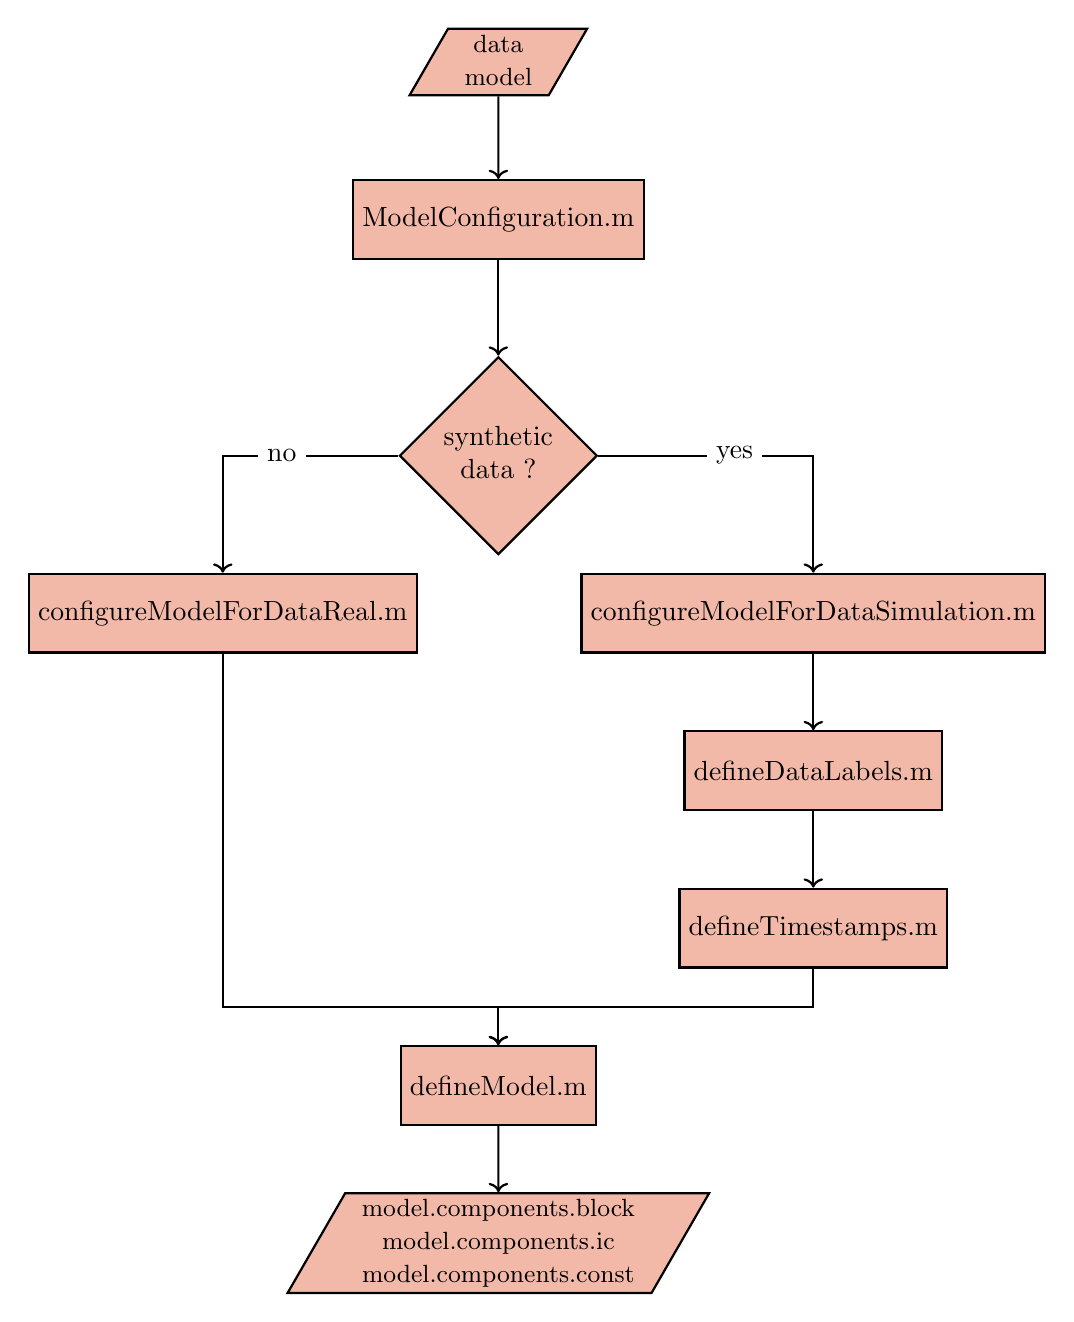
\begin{tikzpicture}

\node[parabisque](inputModelConfiguration){\begin{tabular}{c} \lstinline[basicstyle = \mlttfamily \small ]!data! \\ \lstinline[basicstyle = \mlttfamily \small ]!model! \end{tabular}};
\node[esbisque][below of = inputModelConfiguration, yshift = -1cm ](ModelConfiguration){\phantom{} ModelConfiguration.m \phantom{}};
\node[testbisque](testSimulation)[below of = ModelConfiguration, yshift = -2cm]{\begin{tabular}{c} synthetic \\ data ?  \end{tabular}};
\node[esbisque](ModelConfigurationReal)[below of = testSimulation, yshift = -1cm, xshift = -3.5cm]{\phantom{} configureModelForDataReal.m \phantom{}};
\node[esbisque](ModelConfigurationSimulation)[below of = testSimulation, yshift = -1cm, xshift = 4cm]{\phantom{} configureModelForDataSimulation.m \phantom{}};
\node[esbisque](defineDataLabels)[below of = ModelConfigurationSimulation, yshift = -1cm]{\phantom{} defineDataLabels.m \phantom{}};
\node[esbisque](defineTimestamps)[below of = defineDataLabels, yshift = -1cm]{\phantom{} defineTimestamps.m \phantom{}};
\node[esbisque](defineModel)[below of = ModelConfiguration, yshift = -10cm]{\phantom{} defineModel.m \phantom{}};
\node[parabisque](outputModelConfig)[below of = defineModel, yshift = -1cm]{\begin{tabular}{c} \lstinline[basicstyle = \mlttfamily \small ]!model.components.block! \\ \lstinline[basicstyle = \mlttfamily \small ]!model.components.ic! \\  \lstinline[basicstyle = \mlttfamily \small ]!model.components.const!  \end{tabular}};

\path[->, thick] (inputModelConfiguration)edge(ModelConfiguration);
\path[->, thick] (ModelConfiguration)edge(testSimulation);
\path[->, draw, thick] (testSimulation.west) -| (-2cm,-5cm) -| node[pos=0.25, rotate=0, fill=white]{ no} (ModelConfigurationReal.north);
\path[->, draw, thick] (testSimulation.east) -| (2cm,-5cm) -| node[pos=0.25, rotate=0, fill=white]{ yes} (ModelConfigurationSimulation.north);
\path[->, thick] (ModelConfigurationSimulation)edge(defineDataLabels);
\path[->, thick] (defineDataLabels)edge(defineTimestamps);
\path[->, draw, thick] (defineTimestamps.south) |- (4cm,-12cm) -|  (defineModel.north);
\path[->, draw, thick] (ModelConfigurationReal.south) |- (-3cm,-12cm) -|  (defineModel.north);
\path[->, thick] (defineModel)edge(outputModelConfig);

\end{tikzpicture} } 
\caption{Model configuration workflow} \label{FIG:ModelConfigurationWorkflow}
\end{figure}

\subsection{Model construction}
\label{S:MODELCONSTRUCTION}

%Once the model has been configured, the next step is to build the model.
Model construction builds the full model matrices $A$, $C$, $Q$, $R$ by assembling the sub-matrices associated with each block component and each time-series.
The corresponding values for the model parameters are also considered during model construction.
%Because the model matrices are often time-dependent, OpenBDLM creates a function for each matrix, that depends on the time $t$, and model parameters $\bm\theta$.

\subsubsection{Model construction functions}

The model construction workflow is presented in Figure~\ref{FIG:ModelConstructionWorkflow}. The function in OpenBDLM used for model construction is:

\begin{description}[style=unboxed]
\item[Builds the model ] \leavevmode
  \begin{lstlisting}[ basicstyle = \mlttfamily \small, breaklines=true]
  [model, misc]=buildModel(data, model, misc)
 \end{lstlisting}
\end{description}

\begin{figure}[!h]
  \centering
  \captionsetup{justification=centering}
\scalebox{0.7}{
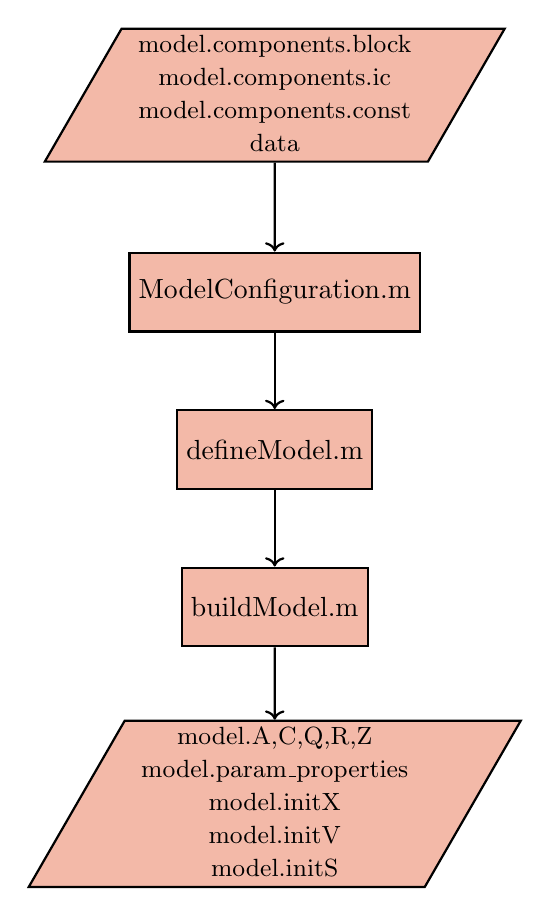
\begin{tikzpicture}


\node[parabisque](inputModelConstruct){\begin{tabular}{c} \lstinline[basicstyle = \mlttfamily \small ]!model.components.block! \\ \lstinline[basicstyle = \mlttfamily \small ]!model.components.ic! \\  \lstinline[basicstyle = \mlttfamily \small ]!model.components.const!  \\ \lstinline[basicstyle = \mlttfamily \small ]!data!  \end{tabular}};
\node[esbisque](ModelConfiguration)[below of = inputModelConstruct, yshift = -1.5cm]{\phantom{} ModelConfiguration.m \phantom{}};
\node[esbisque](defineModel)[below of = ModelConfiguration, yshift = -1cm]{\phantom{} defineModel.m \phantom{}};
\node[esbisque](buildModel)[below of = defineModel , yshift=-1cm, xshift = 0cm]{\phantom{} buildModel.m \phantom{}};

\node[parabisque](outputModelConstruct)[below of = defineModel, yshift = -3.5cm]{\begin{tabular}{c}  \lstinline[basicstyle = \mlttfamily \small ]!model.A,C,Q,R,Z!  \\ \lstinline[basicstyle = \mlttfamily \small ]!model.param_properties! \\ \lstinline[basicstyle = \mlttfamily \small ]!model.initX! \\  \lstinline[basicstyle = \mlttfamily \small ]!model.initV!  \\ \lstinline[basicstyle = \mlttfamily \small ]!model.initS!  \end{tabular}};

\path[->, thick] (inputModelConstruct)edge(ModelConfiguration);
\path[->, thick] (ModelConfiguration)edge(defineModel);
\path[->, thick] (defineModel)edge (buildModel);
\path[->, thick] (buildModel)edge (outputModelConstruct);

\end{tikzpicture} } 
\caption{Model construction workflow} \label{FIG:ModelConstructionWorkflow}
\end{figure}

\subsection{Model parameters estimation}
\label{S:PARAMESTIMATION}

The default values for the parameters are either defined from engineering heuristic knowledge or from statistics computed on the data itself (see~Table \ref{table:defaultparamreal}).
Each value is only an initial guess which has to be refined using an optimization algorithm (see Section~\ref{SS:THModelParameterEstimation}). 
The algorithm will estimate the model parameter values from the data.
% that estimates the model parameters from the data.\\

\begin{table}[h!]
\caption{Default values for model parameters. $\hat{\sigma}_{y_{obs(1:\mathtt{T})}}$ corresponds to the empirical standard deviation calculated using observed data from the first data sample to the last data sample of index $\mathtt{T}$. Note that default value for synthetic data are different, see~Table \ref{table:defaultsynthetic} for details.} 
\centering
\begin{tabular}{r|ll}
\hline
$\bm{\theta}$ name  & $\bm{\theta}^{0}$ & $\bm{\theta}$ bounds \\\cmidrule(lr){1-3}
$\sigma_{w}^{\mathtt{LL}}$  &  $0$ & $[\text{NaN},\text{NaN}]$ \\
$\sigma_{w}^{\mathtt{LT}} $ &  $10^{-7}\times\hat{\sigma}_{y_{obs(1:\mathtt{T})}}$ & $[\text{NaN},\text{NaN}]$ \\
$\sigma_{w}^{\mathtt{LA}} $ &  $10^{-8}\times\hat{\sigma}_{y_{obs(1:\mathtt{T})}}$ & $[\text{NaN},\text{NaN}]$ \\
$\sigma_{w}^{\mathtt{LcT}} $ &  $10^{-7}\times\hat{\sigma}_{y_{obs(1:\mathtt{T})}}$ & $[\text{NaN},\text{NaN}]$ \\
$\sigma_{w}^{\mathtt{LcA}} $ &  $10^{-7}\times\hat{\sigma}_{y_{obs(1:\mathtt{T})}}$ & $[\text{NaN},\text{NaN}]$ \\
$\sigma_{w}^{\mathtt{TcA}} $ &  $10^{-8}\times\hat{\sigma}_{y_{obs(1:\mathtt{T})}}$ & $[\text{NaN},\text{NaN}]$ \\
$\sigma_{w}^{\mathtt{P}} $ &  $0$ & $[\text{NaN},\text{NaN}]$ \\
$\sigma_{w}^{\mathtt{AR}} $ &  $10^{-1}\times\hat{\sigma}_{y_{obs(1:\mathtt{T})}}$ & $[0,\text{Inf}]$ \\
$\sigma_{w,0}^{\mathtt{KR}}  $ &  $10^{-1}\times\hat{\sigma}_{y_{obs(1:\mathtt{T})}}$  & $[0,\text{Inf}]$ \\
$\sigma_{w,1}^{\mathtt{KR}}  $ &  $0$  &  $[\text{NaN},\text{NaN}]$ \\
$\sigma_{v}$ &  $0.05\times\hat{\sigma}_{y_{obs(1:\mathtt{T})}}$  &  $[0,\text{Inf}]$ \\
$\phi^{\mathtt{AR}} $ &  $0.75$ & $[0,1]$ \\
$p^{\mathtt{P}} $ &  $[365.24, 1, 182.62]$\footnote{One different default value for the period is given for each periodic component.} & $[\text{NaN},\text{NaN}]$ \\
$p^{\mathtt{KR}} $ &  $365.24$ & $[\text{NaN},\text{NaN}]$ \\
$\ell^{\mathtt{KR}} $ &  $2/\mathtt{L}^{\mathtt{KR}}$ (see \S\ref{SSS:KR})& $[0,\text{Inf}]$ \\
$\phi^{\cdot|\cdot} $ &  $0.01$  &  $[-\text{Inf}, \text{Inf}]$\\\hline
\end{tabular}
\label{table:defaultparamreal}
\end{table}



In order to access the model parameter estimation menu from OpenBDLM, type  \colorbox{light-gray}{\lstinline[basicstyle = \mlttfamily \small, backgroundcolor = \color{light-gray}]!1!} (see Listing~\ref{LST:ModelParametersEstimationMenu}).
The optimization algorithm is either the Newton-Raphson (choice \colorbox{light-gray}{\lstinline[basicstyle = \mlttfamily \small, backgroundcolor = \color{light-gray}]!1!}) or the Stochastic Gradient Descent  (choice \colorbox{light-gray}{\lstinline[basicstyle = \mlttfamily \small, backgroundcolor = \color{light-gray}]!2!}) algorithms (see Section~\ref{SS:THModelParameterEstimation}).
By default, OpenBDLM uses all the data as the training set (see \lstinline[basicstyle = \mlttfamily \small ]!misc.options.Trainingperiod=[1 Inf]!).
OpenBDLM transform the model parameters to perform the optimization in an unbounded model parameter space (see Section~\ref{SS:THSpaceTransformation}).
Undefined bounds (\lstinline[basicstyle = \mlttfamily \small ]![NaN, NaN]!)  for a parameter means that the parameter is assumed to be known and thus, it will be excluded from the parameter estimation process.
By default, OpenBLDM assumes that all parameters are unknown, except for the period of the periodic component and the process noise standard deviation associated with the baseline and the periodic component.
Those model parameters have values fixed to 0.\\

The model parameter can be learned by maximizing either the likelihood (Maximum Likelihood Estimation, MLE), or the posterior function (Maximum A Posteriori estimation, MAP) (see Section~\ref{SS:THModelParameterEstimation}). 
Note that MAP requires a valid prior for each unknown model parameters.
In the case of of MAP, OpenBDLM supports gaussian prior only.
The default option is MLE (see \lstinline[basicstyle = \mlttfamily \small ]!misc.options.isMAP=false!).
There is the possibility to use the prediction capacity to drive the optimization process\footnote{The use of the prediction capacity is only available using the Stochastic Gradient Descent optimization.} (see  \lstinline[basicstyle = \mlttfamily \small ]!misc.options.isPredCap! and \lstinline[basicstyle = \mlttfamily \small ]!misc.options.SplitPercent!).
\begin{lstlisting}[ frame = single, basicstyle = \mlttfamily \small, caption = {OpenBDLM model parameter estimation menu}, label = LST:ModelParametersEstimationMenu ,  float =ht, linewidth=\linewidth, captionpos=b]
-------------------------------------------
/ Learn model parameters
-------------------------------------------

     1 ->  Newton-Raphson
     2 ->  Stochastic Gradient Ascent

     Type R to return to the previous menu

     choice >> 
\end{lstlisting}
The model parameter estimation framework computes point estimate of the model parameters. 
However, it is also possible provide confidence intervals around the point estimate using the Laplace approximation\footnote{Laplace approximation is currently only available using the Newton-Raphson optimization.} (see \lstinline[basicstyle = \mlttfamily \small ]!misc.options.isLaplaceApproximation = true!).
Note that computing the Laplace approximation can significantly increase the computation time and it is not recommended when the number of model parameters is large.\\

Note also that Newton-Raphson and Stochastic Gradient Descent techniques are sensitive to the initial model parameters values. 
%The algorithm can reach a local maximum, instead of the global maximum.
Therefore, it is advised to run the optimizations several times with different starting model parameters values in order to check if the proposed solution is the best attainable solution.
If \lstinline[basicstyle = \mlttfamily \small ]!misc.options.isMute = false!, outputs on the \MATLAB{} command line window allow to monitor the optimization process (see Listings~\ref{LST:OpenBLDMModelParameterLearning}-\ref{LST:OpenBLDMModelParameterLearningSGD}).
At each iteration, the quantity displayed are: the current value of the target function, the name as well as the current value of the unknown model parameter being optimized, the change in model parameters, the change in the target function, and the convergence status (\lstinline[basicstyle = \mlttfamily \small ]!1! if the model parameter converged according to the convergence criteria, \lstinline[basicstyle = \mlttfamily \small ]!0! otherwise).\\

The optimization stops when all the parameters converged, or if the maximum number of iterations (see \lstinline[basicstyle = \mlttfamily \small ]!misc.options.maxIterations!) (or epochs for Stochastic Gradient Descent algorithm, see \lstinline[basicstyle = \mlttfamily \small ]!misc.options.maxEpochs!) / the maximum time (see \lstinline[basicstyle = \mlttfamily \small ]!misc.options.maxTime!) is reached.
The values of the parameters are saved in the variable \lstinline[basicstyle = \mlttfamily \small ]!model! \MATLAB{}.
 
 \begin{lstlisting}[ frame = single, basicstyle = \mlttfamily \small, caption = {OpenBLDM output example when running Newton-Raphson algorithm.}, label = LST:OpenBLDMModelParameterLearning,  float =h!, linewidth=\linewidth, captionpos=b]
    \Start Newton-Raphson max. algorithm (finite difference method)

      Training period:                             1-Inf [days]
      Maximal number of iteration:                 100
      Total time limit for calibration :           60 [min]
      Convergence criterion:                       1e-07*LL
      Nb. of search levels for \lambda:            4*2

           Initial LL: 36626.8381
                       AR|M1|1         AR|M1|1         |M1|1            
      parameter names: \phi            \sigma_w        \sigma_v         
       initial values: +7.50e-01       +1.74e-02       +8.70e-03       
--------------------------
    Loop #1 : |M1|1 | \sigma_v 
       delta_param: -0.0040755 
    log-likelihood : 36994.6374
    param change   : 0.0087002 -> 0.0046247

                    AR|M1|1         AR|M1|1         |M1|1           
   parameter names: \phi            \sigma_w        \sigma_v        
    current values: +7.50e-01       +1.74e-02       +4.62e-03      
  current f.o. std: +0.00e+00       +0.00e+00       +1.93e-04      
      previous dLL: +1.00e+06       +1.00e+06       +3.68e+02      
         converged:         0               0               0      
--------------------------
    Loop #2 : AR|M1|1 | \sigma_w 
       delta_param: 0.0046034 
    log-likelihood : 40998.3934
    param change   : 0.0174 -> 0.022003

                    AR|M1|1         AR|M1|1         |M1|1           
   parameter names: \phi            \sigma_w        \sigma_v        
    current values: +7.50e-01       +2.20e-02       +4.62e-03      
  current f.o. std: +0.00e+00       +5.26e-05       +1.93e-04      
      previous dLL: +1.00e+06       +4.00e+03       +3.68e+02      
         converged:         0               0               0      
--------------------------
\end{lstlisting}



 \begin{lstlisting}[ frame = single, basicstyle = \mlttfamily \small, caption = {OpenBLDM output example when running Stochastic Gradient Ascent algorithm.}, label = LST:OpenBLDMModelParameterLearningSGD,  float =h!, linewidth=\linewidth, captionpos=b]
    \Start SGD algorithm (finite difference method)

      Optimization mode                           MLE
      Optimizer                                   MMT
      Metric                                      logpdf
      Learning Rate mode                          hessian
      Training period:                            1 - Inf [days]
      Validation set portion:                     30 [%]
      Training set:                               13556 [data points]
      Validation set:                             5810 [data points]
      Mini batch:                                 3873 [data points]
      Number of max epoch:                        30+1 [epochs]
      Total time limit for calibration:           60 [min]

    Epoch #1
             Metric: 25972.5904
                    AR|M1|1         AR|M1|1         |M1|1           
   parameter names: \phi            \sigma_w        \sigma_v        
    initial values: +7.50e-01       +1.74e-02       +8.70e-03       

--------------------------
    Epoch #2
            Metric: 33933.8856
   parameter names: AR|M1|1         AR|M1|1         |M1|1           
    current values: +9.61e-01       +2.00e-02       +5.66e-03      
      param change: +2.11e-01       +2.61e-03       -3.04e-03      
  initialize param:         0               0               0      


--------------------------
    Epoch #3
            Metric: 33933.8856
   parameter names: AR|M1|1         AR|M1|1         |M1|1           
    current values: +9.61e-01       +2.00e-02       +5.66e-03      
      param change: +0.00e+00       +0.00e+00       +0.00e+00      
  initialize param:         1               0               0 
\end{lstlisting}










\subsubsection{Model parameter estimation functions}

\begin{description}[style=unboxed]
\item[Pilot function for optimization] \leavevmode
  \begin{lstlisting}[ basicstyle = \mlttfamily \small, breaklines=true]
[data,model,estimation,misc]=piloteOptimization(data,model,estimation,misc)
  \end{lstlisting}

\item[Estimates model parameter using Newton-Raphson algorithm] \leavevmode
  \begin{lstlisting}[ basicstyle = \mlttfamily \small, breaklines=true]
[optim,model]=NewtonRaphson(data,model,misc)
  \end{lstlisting}
  
 \item[Estimates model parameter using Stochastic Gradient Descent algorithm] \leavevmode
  \begin{lstlisting}[ basicstyle = \mlttfamily \small, breaklines=true]
[optim,model] = SGD(data,model,misc,varargin)
  \end{lstlisting} 

 \item[Reads model parameter properties ] \leavevmode
 \begin{lstlisting}[ basicstyle = \mlttfamily \small, breaklines=true]
[arrayOut]=readParameterProperties(cellIn,Position)
  \end{lstlisting} 

 \item[Writes model parameter properties ] \leavevmode
 \begin{lstlisting}[ basicstyle = \mlttfamily \small, breaklines=true]
[cellOut]=writeParameterProperties(cellIn,arrayIn,Position)
  \end{lstlisting} 

 \item[Approximates the target function, as well as the first and second derivative of the logarithm of the target function with respect to parameter values ] \leavevmode
  \begin{lstlisting}[ basicstyle = \mlttfamily \small, breaklines=true]
[logpdf,Glogpdf,Hlogpdf, delta_grad] = logPosteriorPE(data,model,misc,varargin)
  \end{lstlisting} 

 \item[Computes the gradient and hessian of the gaussian prior distribution of each model parameter ] \leavevmode
  \begin{lstlisting}[ basicstyle = \mlttfamily \small, breaklines=true]
[logprior,Glogprior,Hlogprior]= logPriorDistr(P,Mu,Sigma,varargin)
  \end{lstlisting} 

 \item[Computes numerical hessian H of a function ] \leavevmode
  \begin{lstlisting}[ basicstyle = \mlttfamily \small, breaklines=true]
H=numerical_hessian(x,fX,varargin)
  \end{lstlisting} 

 \item[Defines transformation functions and their derivatives according to provided bounds for the model parameters ] \leavevmode
  \begin{lstlisting}[ basicstyle = \mlttfamily \small, breaklines=true]
[fct_TR,fct_inv_TR,grad_TR2OR,hessian_TR2OR]=parameter_transformation_fct(model,param_idx_loop)
  \end{lstlisting} 

 \item[Performs Switching Kalman filter on time series ] \leavevmode
  \begin{lstlisting}[ basicstyle = \mlttfamily \small, breaklines=true]
[x,V,VV,S,loglik,U,D]=SwitchingKalmanFilter(data,model,misc)
  \end{lstlisting} 

 \item[Computes the first and second derivative of the logarithm of the likelihood function with respect to parameter values] \leavevmode
 \begin{lstlisting}[ basicstyle = \mlttfamily \small, breaklines=true]
[grad,hessian,fail_gradHess,delta_grad] = gradHess(data, model,misc,pTR,pOR,log_lik_0,grad_TR2OR,delta_grad,param_idx_loop)
 \end{lstlisting} 

 \item[Computes the optimal parameter step size for the approximation of the numerical derivative of the likelihood and compute the terms required to approximate the numerical derivative using finite differene method] \leavevmode
 \begin{lstlisting}[ basicstyle = \mlttfamily \small, breaklines=true]
[delta_grad,fail_delta_grad,log_lik_1,log_lik_2] = StepSizeOptimization(model,data,misc,pOR,log_lik_0,delta_grad,param_idx_loop)
 \end{lstlisting} 

 \item[Splits the full dataset into train and test dataset (for Stochastic Gradient Descent only) ] \leavevmode
  \begin{lstlisting}[ basicstyle = \mlttfamily \small, breaklines=true]
[data_train,data_valid] = dataSplit(data,idxTrain,alpha_split,varargin)
  \end{lstlisting} 

 \item[Computes the metric function (for Stochastic Gradient Descent only) ] \leavevmode
  \begin{lstlisting}[ basicstyle = \mlttfamily \small, breaklines=true]
[metricVL,idxMaxM,logpdf_test,logpdf_train] = metricFct(data_train,data_test,model,misc,parameterSearch,parameterSearchTR)
  \end{lstlisting} 

 \item[paramGrid (for Stochastic Gradient Descent only) ] \leavevmode
  \begin{lstlisting}[ basicstyle = \mlttfamily \small, breaklines=true]
[xM,momentumM,RMSpropM,gradM,learningRateM, mmtHessM, hessM]= paramGrid(x,momentum,RMSprop,grad,learningRate,mmtHess,hess)
  \end{lstlisting} 
  
  \item[ADAM optimizer (for Stochastic Gradient Descent only)] \leavevmode
  \begin{lstlisting}[ basicstyle = \mlttfamily \small, breaklines=true]
[xsearch,xsearchTR,momentumTR,RMSpropTR] = ADAM(xsearchTRprev,momentumTRprev,RMSpropTRprev,grad,step,beta_1,beta_2,epsilon,Niter,fctInvTR)  
  \end{lstlisting} 
    
\item[MMT optimizer (for Stochastic Gradient Descent only)] \leavevmode
  \begin{lstlisting}[ basicstyle = \mlttfamily \small, breaklines=true]
[xsearch,xsearchTR,momentumTR] = MMT(xsearchTRprev,momentumTRprev,grad,step,beta,fctInvTR)
\end{lstlisting} 
    
  
\end{description}

\begin{figure}[!h]
  \centering
  \captionsetup{justification=centering}
\scalebox{0.8}{
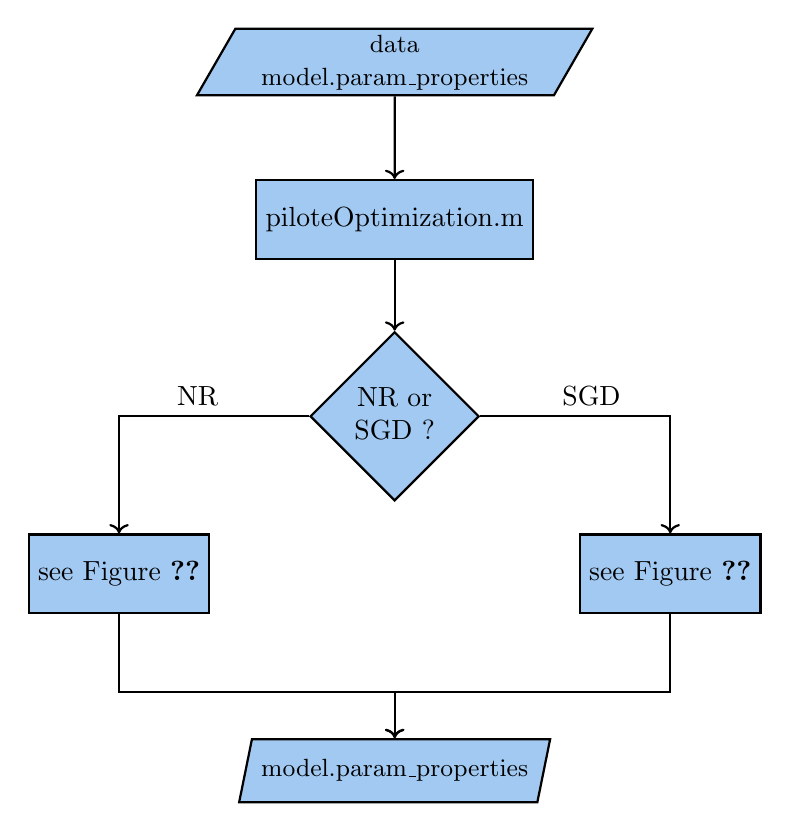
\begin{tikzpicture}

\node[parababyblueeyes](inputOptimization){ \begin{tabular}{c} \lstinline[ basicstyle = \mlttfamily \small]!data! \\ \phantom{}  \lstinline[ basicstyle = \mlttfamily \small]!model.param_properties! \phantom{} \end{tabular}};
\node[esbabyblueeyes](piloteOptimization)[below of = inputOptimization, yshift = -1cm]{\phantom{} piloteOptimization.m \phantom{}};
\node[testbabyblueeyes](testNRSGD)[below of = piloteOptimization, yshift = -1.5cm]{\begin{tabular}{c} NR or  \\ SGD ?  \end{tabular}};
\node[esbabyblueeyes](SeeNewtonRaphson)[below of = testNRSGD, yshift = -1cm, xshift = -3.5cm]{\phantom{} see Figure~\ref{FIG:NewtonRaphsonWorkflow} \phantom{}};
\node[esbabyblueeyes](SeeSGD)[below of = testNRSGD, yshift = -1cm, xshift = 3.5cm]{\phantom{} see Figure~\ref{FIG:SGDWorkflow} \phantom{}};
\node[parababyblueeyes](outputOptimization)[below of = inputOptimization, yshift = -8cm]{\phantom{}  \lstinline[ basicstyle = \mlttfamily \small]!model.param_properties! \phantom{}};

\path[->, draw, thick] (inputOptimization)edge(piloteOptimization);
\path[->, draw, thick] (piloteOptimization)edge(testNRSGD);
\path[->, draw, thick] (testNRSGD.east) -| (1.5cm,-4.5cm) -| node[pos=0.25, above]{ SGD} (SeeSGD.north);
\path[->, draw, thick] (testNRSGD.west) -| (-1.5cm,-4.5cm) -| node[pos=0.25, above]{NR} (SeeNewtonRaphson.north);
\path[->, draw, thick] (SeeNewtonRaphson.south) |- (0cm,-8cm) -|  (outputOptimization.north);
\path[->, draw, thick] (SeeSGD.south) |- (0cm,-8cm) -|  (outputOptimization.north);
\end{tikzpicture} } 
\caption{Model parameter estimation workflow} \label{FIG:ModelParameterEstimationWorkflow}
\end{figure}


\begin{figure}[!h]
  \centering
  \captionsetup{justification=centering}
\scalebox{0.8}{
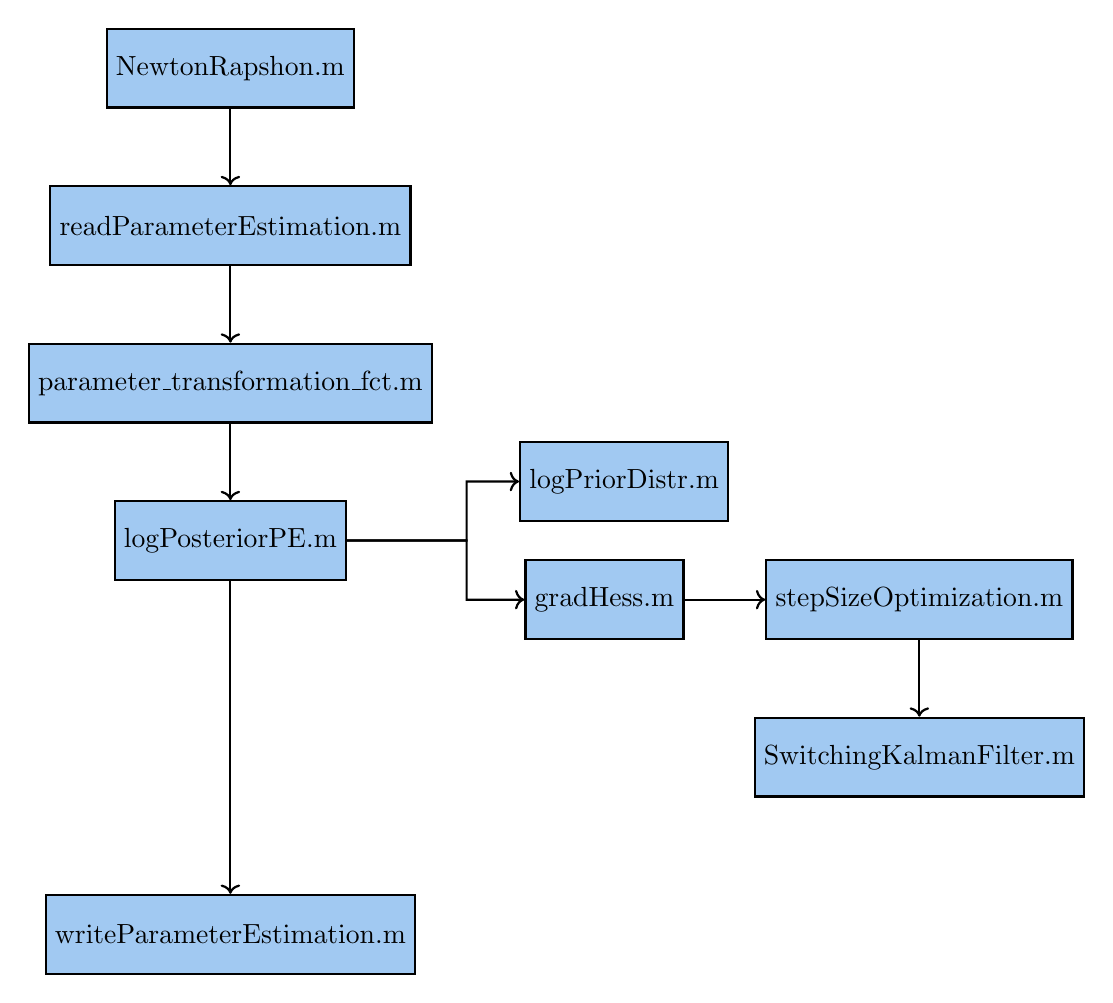
\begin{tikzpicture}

\node[esbabyblueeyes](NewtonRaphson){\phantom{} NewtonRapshon.m \phantom{}};
\node[esbabyblueeyes](readParameterEstimation)[below of = NewtonRaphson, yshift = -1cm]{\phantom{} readParameterEstimation.m \phantom{}};
\node[esbabyblueeyes](paramtransform)[below of = readParameterEstimation , yshift = -1cm]{\phantom{}  parameter\_transformation\_fct.m \phantom{}};
\node[esbabyblueeyes](logposterior)[below of = paramtransform  , yshift = -1cm]{\phantom{}  logPosteriorPE.m \phantom{}};
\node[esbabyblueeyes](logPrior)[right of = logposterior , xshift=4cm, yshift = 0.75cm]{\phantom{}  logPriorDistr.m \phantom{}};
\node[esbabyblueeyes](gradHess)[right of = logposterior , xshift=3.75cm, yshift = -0.75cm]{\phantom{}  gradHess.m \phantom{}};
\node[esbabyblueeyes](SSO)[right of = gradHess , xshift=3cm, yshift = 0cm]{\phantom{}  stepSizeOptimization.m \phantom{}};
\node[esbabyblueeyes](SKF)[below of = SSO , xshift=0cm, yshift = -1cm]{\phantom{}  SwitchingKalmanFilter.m \phantom{}};
\node[esbabyblueeyes](writeParameterEstimation)[below of = logposterior, yshift = -4cm]{\phantom{} writeParameterEstimation.m \phantom{}};


\path[->, draw, thick] (NewtonRaphson)edge(readParameterEstimation);
\path[->, draw, thick] (readParameterEstimation)edge(paramtransform);
\path[->, draw, thick] (paramtransform)edge(logposterior);
\path[->, draw, thick] (logposterior.east) -| (3cm,-5.25cm) --  (logPrior.west);
\path[->, draw, thick] (logposterior.east) -| (3cm,-6.75cm) --  (gradHess.west);
\path[->, draw, thick] (gradHess)edge(SSO);
\path[->, draw, thick] (SSO)edge(SKF);
\path[->, draw, thick] (logposterior)edge(writeParameterEstimation);

\end{tikzpicture} } 
\caption{Model parameter estimation Newton-Raphson workflow} \label{FIG:NewtonRaphsonWorkflow}
\end{figure}


\begin{figure}[h]
  \centering
  \captionsetup{justification=centering}
\scalebox{0.8}{
\begin{tikzpicture}

\node[esbabyblueeyes](SGD){\phantom{} SGD.m \phantom{}};
\node[esbabyblueeyes](readParameterEstimation)[below of = SGD, yshift = -1cm]{\phantom{} readParamaterEstimation.m \phantom{}};
\node[esbabyblueeyes](paramtransform)[below of = readParameterEstimation , yshift = -1cm]{\phantom{}  parameter\_transformation\_fct.m \phantom{}};
\node[esbabyblueeyes](metric1)[below of = paramtransform , yshift = -1cm]{\phantom{}  metricFct.m \phantom{}};
\node[esbabyblueeyes](split)[below of =metric1 , yshift = -1cm]{\phantom{}  dataSplit.m \phantom{}};
\node[esbabyblueeyes](logposterior)[below of = split  , yshift = -1cm]{\phantom{}  logPosteriorPE.m \phantom{}};
\node[esbabyblueeyes](logPrior)[right of = logposterior , xshift=4cm, yshift = 0.75cm]{\phantom{}  logPriorDistr.m \phantom{}};
\node[esbabyblueeyes](gradHess)[right of = logposterior , xshift=3.75cm, yshift = -0.75cm]{\phantom{}  gradHess.m \phantom{}};
\node[esbabyblueeyes](SSO)[right of = gradHess , xshift=3cm, yshift = 0cm]{\phantom{}  stepSizeOptimization.m \phantom{}};
\node[esbabyblueeyes](SKF)[below of = SSO , xshift=0cm, yshift = -1cm]{\phantom{}  SwitchingKalmanFilter.m \phantom{}};
\node[esbabyblueeyes](grid)[below of = logposterior, yshift = -3.5cm]{\phantom{} paramGrid.m \phantom{}};
\node[esbabyblueeyes](adam)[below of = grid, yshift = -1cm]{\phantom{} \begin{tabular}{c} ADAM.m  \\ MMT.m  \end{tabular}};
\node[esbabyblueeyes](metric2)[below of = adam , yshift = -1cm]{\phantom{}  metricFct.m \phantom{}};
\node[esbabyblueeyes](writeParameterEstimation)[below of = metric2, yshift = -1cm]{\phantom{} writeParameterEstimation.m \phantom{}};


\path[->, draw, thick] (NewtonRaphson)edge(readParameterEstimation);
\path[->, draw, thick] (readParameterEstimation)edge(paramtransform);
\path[->, draw, thick] (paramtransform)edge(metric1);
\path[->, draw, thick] (metric1)edge(split);
\path[->, draw, thick] (split)edge(logposterior);
\path[->, draw, thick] (logposterior.east) -| (3cm,-9.25cm) --  (logPrior.west);
\path[->, draw, thick] (logposterior.east) -| (3cm,-10.75cm) --  (gradHess.west);
\path[->, draw, thick] (gradHess)edge(SSO);
\path[->, draw, thick] (SSO)edge(SKF);
\path[->, draw, thick] (logposterior)edge(grid);
\path[->, draw, thick] (grid)edge(adam);
\path[->, draw, thick] (adam)edge(metric2);
\path[->, draw, thick] (metric2)edge(writeParameterEstimation);

\end{tikzpicture} } 
\caption{Model parameter estimation Stochastic gradient descent workflow} \label{FIG:SGDWorkflow}
\end{figure}

\subsection{Hidden states estimation}
\label{S:HIDDENSTATESESTIMATION}

The estimation of the hidden states is the core of OpenBLDM.
%Each hidden state belongs to a block component used to build the model.
The hidden state estimation is performed recursively using the Kalman filter/smoother or the UD filter/smoother (see Section~\ref{SS:KFUD}).
Once a project is loaded, typing \colorbox{light-gray}{\lstinline[basicstyle = \mlttfamily \small ]!3!} opens the hidden state estimation menu (see Listing~\ref{LST:StateEstimationMenu}).

\begin{lstlisting}[ frame = single, basicstyle = \mlttfamily \small, caption = {OpenBDLM hidden states estimation menu}, label = LST:StateEstimationMenu ,  float =ht, linewidth=\linewidth, captionpos=b]
---------------------------------------------------
/    State estimation
---------------------------------------------------

     1 ->  Filter 
     2 ->  Smoother 

     Type R to return to the previous menu 

     choice >> 
\end{lstlisting}

Type  \colorbox{light-gray}{\lstinline[basicstyle = \mlttfamily \small ]!1!} runs the Kalman or UD filter, and typing \colorbox{light-gray}{\lstinline[basicstyle = \mlttfamily \small ]!2!} runs the Kalman or UD smoother.
The Kalman is the default state estimation method (see \lstinline[basicstyle = \mlttfamily \small ]!misc.options.MethodStateEstimation!), but UD computations are more stable in particular in the case of missing data or in case of a sudden increase of the time step.

\subsubsection{Hidden state estimation functions}

The hidden state estimation workflow is presented Figure~\ref{FIG:HiddenStateEstimationWorkflow}.
The OpenBLDM functions used for hidden state estimation are:

\begin{description}[style=unboxed]
\item[Pilote function for hidden state estimation] \leavevmode
  \begin{lstlisting}[ basicstyle = \mlttfamily \small, breaklines=true]
[data,model,estimation,misc]=piloteStateEstimation(data,model,estimation,misc)
  \end{lstlisting}

\item[Runs state estimation] \leavevmode
  \begin{lstlisting}[ basicstyle = \mlttfamily \small, breaklines=true]
[estimation]=StateEstimation(data,model,misc,varargin)
  \end{lstlisting}

\item[Runs switching Kalman filter for all time] \leavevmode
  \begin{lstlisting}[ basicstyle = \mlttfamily \small, breaklines=true]
[x,V,VV,S,loglik,U,D]=SwitchingKalmanFilter(data,model,misc)
  \end{lstlisting}

\item[Performs Rauch-Tung-Striebel switching smoother for all time] \leavevmode
  \begin{lstlisting}[ basicstyle = \mlttfamily \small, breaklines=true]
[x,V,VV,S,x_prior_smoothed,V_prior_smoothed,VV_prior_smoothed,S_prior_smoothed]=RTS_SwitchingKalmanSmoother(data,model,estimation)
  \end{lstlisting}

\item[Performs one step of the Kalman filter] \leavevmode
  \begin{lstlisting}[ basicstyle = \mlttfamily \small, breaklines=true]
[xnew,Vnew,VVnew,loglik]=KalmanFilter(A,C,Q,R,y,x,V,varargin)
  \end{lstlisting}

\item[Performs one step of the UD filter] \leavevmode
  \begin{lstlisting}[ basicstyle = \mlttfamily \small, breaklines=true]
[xnew,Vnew,VVnew,U_post,D_post,loglik]=UDFilter(A,C,Q,R,y,x,V,U_post,D_post)
  \end{lstlisting}

\item[Computes UD decomposition] \leavevmode
  \begin{lstlisting}[ basicstyle = \mlttfamily \small, breaklines=true]
[U,D] = myUD(mat,varargin)
  \end{lstlisting}
\end{description}



\begin{figure}[h]
  \centering
  \captionsetup{justification=centering}
\scalebox{0.8}{
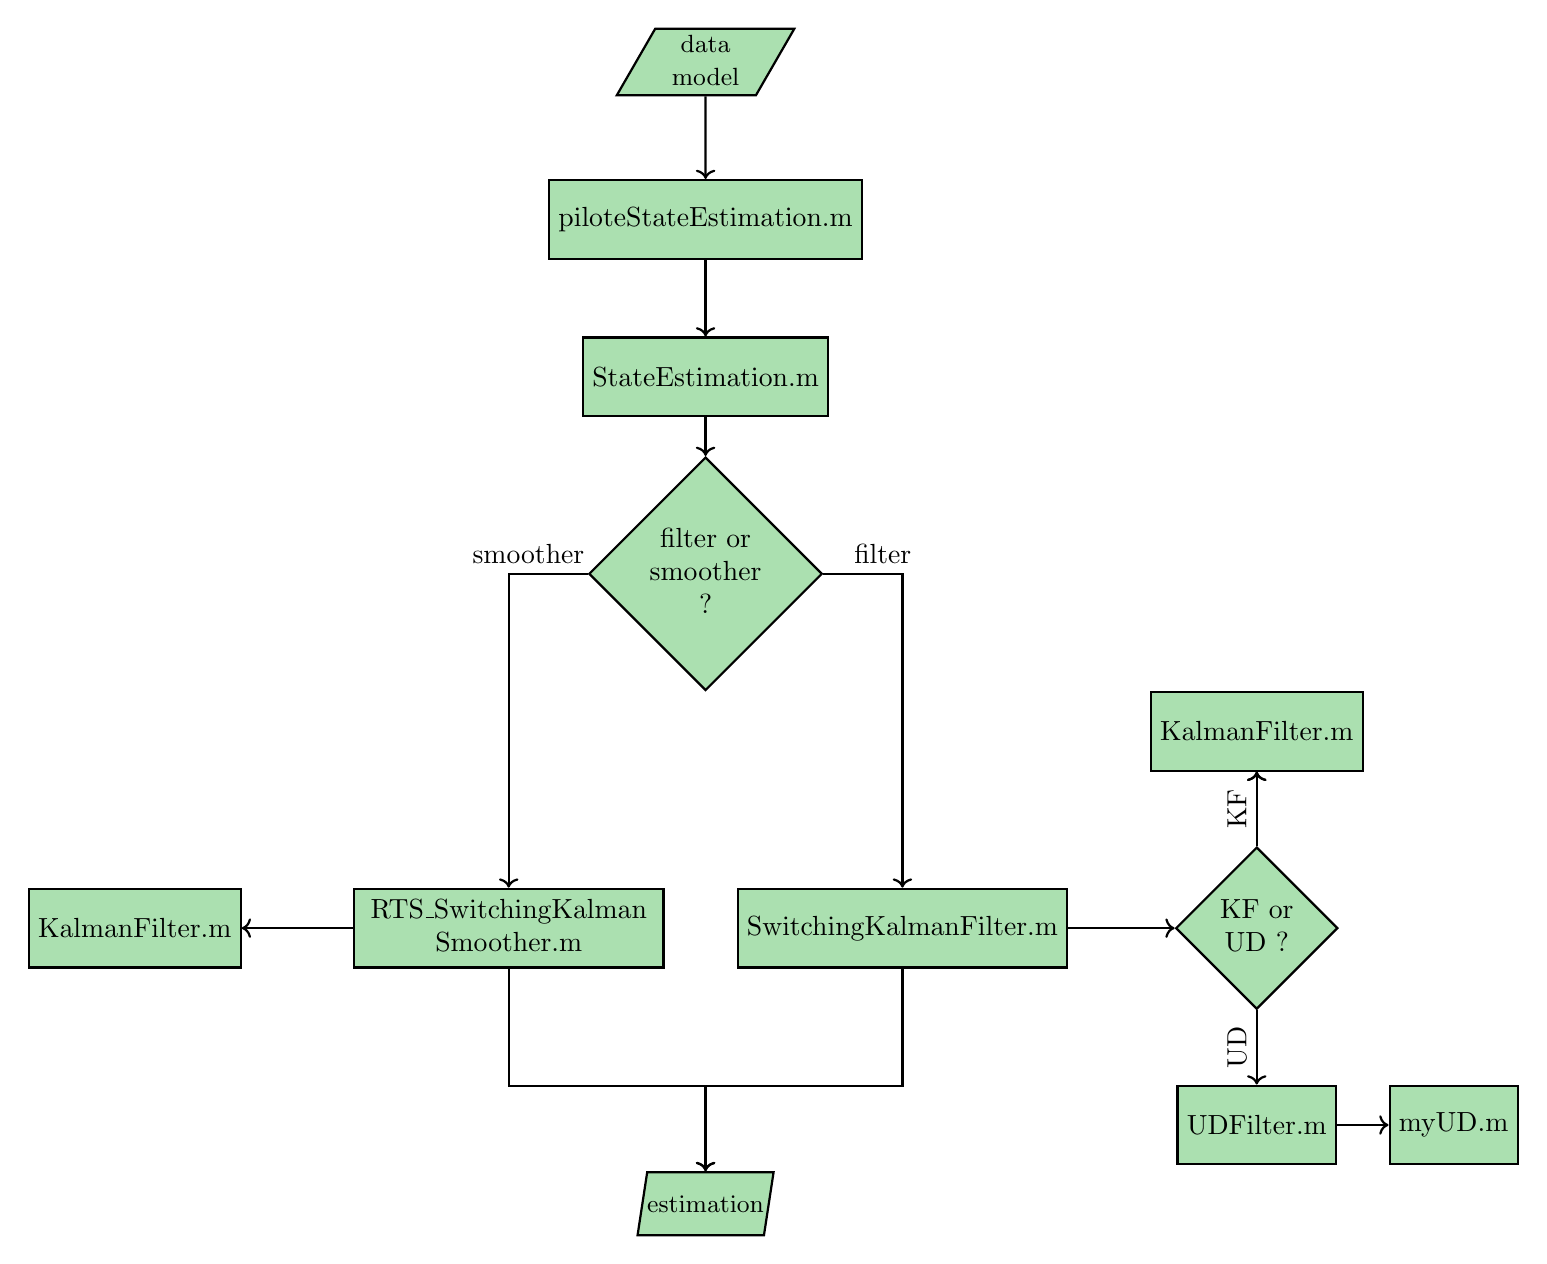
\begin{tikzpicture}

\node[paraceladon](inputHSE){\begin{tabular}{c}  \lstinline[ basicstyle = \mlttfamily \small]!data! \\ \lstinline[ basicstyle = \mlttfamily \small]!model! \end{tabular}};
\node[esceladon](piloteSE)[below of = inputHSE, yshift = -1cm]{\phantom{} piloteStateEstimation.m \phantom{}};
\node[esceladon](SE)[below of = piloteSE, yshift = -1cm]{\phantom{} StateEstimation.m \phantom{}};
\node[testceladon](testSKSSKF)[below of = SE, yshift = -1.5cm]{\begin{tabular}{c} filter or  \\ smoother \\ ?  \end{tabular}};
\node[esceladon](RTS)[below of = testSKSSKF, yshift = -3.50cm, xshift = -2.5cm]{\begin{tabular}{c} RTS\_SwitchingKalman \\ Smoother.m \end{tabular}}; %{\phantom{} RTS\_SwitchingKalmanSmoother.m \phantom{}};
\node[esceladon](KFRTS)[left of = RTS, yshift = 0cm, xshift = -3.75cm]{\phantom{} KalmanFilter.m \phantom{}};
\node[esceladon](SKF)[below of = testSKSSKF , yshift = -3.50cm, xshift = 2.5cm]{\phantom{} SwitchingKalmanFilter.m \phantom{}};
\node[testceladon](testUDKF)[right of = SKF , yshift = 0cm, xshift = 3.5cm]{\begin{tabular}{c} KF or  \\ UD ? \end{tabular}};
\node[esceladon](UDF)[below of = testUDKF, yshift = -1.5cm]{\phantom{} UDFilter.m \phantom{}};
\node[esceladon](myUD)[right of = UDF, yshift = 0cm, xshift=1.5cm]{\phantom{} myUD.m \phantom{}};
\node[esceladon](KF)[below of = testUDKF, yshift = 3.5cm]{\phantom{} KalmanFilter.m \phantom{}};
\node[paraceladon](outputHSE)[below of = inputHSE, yshift = -13.5cm]{\lstinline[ basicstyle = \mlttfamily \small]!estimation!};
%
\path[->, draw, thick] (inputHSE)edge(piloteSE);
\path[->, draw, thick] (piloteSE)edge(SE);
\path[->, draw, thick] (SE)edge(testSKSSKF);
\path[->, draw, thick] (RTS)edge(KFRTS);
\path[->, draw, thick] (testSKSSKF.east) -| (2cm,-6.5cm) -| node[pos=0.25, above]{filter} (SKF);
\path[->, draw, thick] (testSKSSKF.west) -| (-2cm,-6.5cm) -| node[pos=0.25, above]{smoother} (RTS);
\path[->, draw, thick] (SKF.south) |- (0cm,-13cm) -|  (outputHSE.north);
\path[->, draw, thick] (RTS.south) |- (0cm,-13cm) -|  (outputHSE.north);
\path[->, draw, thick] (SKF)edge(testUDKF);
\path[->, draw, thick] (testUDKF)edge(KF);
\path[->, draw, thick] (testUDKF)edge node[anchor=center, above, rotate=90]{KF} (KF);
\path[->, draw, thick] (testUDKF)edge node[anchor=center, above, rotate=90]{UD} (UDF);
\path[->, draw, thick] (UDF)edge(myUD);
\end{tikzpicture} } 
\caption{Hidden states estimation workflow} \label{FIG:HiddenStateEstimationWorkflow}
\end{figure}


\subsubsection{Estimation of the initial hidden states}

OpenBDLM computes default values for the initial (at $t=0$) mean (\lstinline[ basicstyle = \mlttfamily \small]!model.initX!) and covariance (\lstinline[ basicstyle = \mlttfamily \small]!model.initV!) value, as well as the initial model probabilities (\lstinline[ basicstyle = \mlttfamily \small]!model.initS! . %only in the case of $\mathtt{S}=2$ model classes).
Those initial values are usually poor guesses, which may be refined using Kalman smoothing up to $t=0$.
The percent of data used to estimate initial hidden states using Kalman smoothing is controlled by the value provided in \lstinline[ basicstyle = \mlttfamily \small]!misc.options.DataPercent!.
From the OpenBDLM main menu, type \colorbox{light-gray}{\lstinline[basicstyle = \mlttfamily \small, backgroundcolor = \color{light-gray}]!2!}  in the \MATLAB{} command window to estimate the initial hidden states using Kalman smoothing.

The hidden state estimation workflow is presented Figure~\ref{FIG:InitialHiddenStateEstimationWorkflow}. 
The OpenBLDM functions used for initial hidden state estimation are:

\begin{description}[style=unboxed]
\item[Pilote function for initial state estimation] \leavevmode
  \begin{lstlisting}[ basicstyle = \mlttfamily \small, breaklines=true]
[data,model,estimation,misc]=piloteInitialStateEstimation(data,model,estimation,misc)
  \end{lstlisting}

\item[Runs state estimation] \leavevmode
  \begin{lstlisting}[ basicstyle = \mlttfamily \small, breaklines=true]
[estimation]=StateEstimation(data,model,misc,varargin)
  \end{lstlisting}

\item[Performs Rauch-Tung-Striebel switching smoother for all time] \leavevmode
  \begin{lstlisting}[ basicstyle = \mlttfamily \small, breaklines=true]
[x,V,VV,S,x_prior_smoothed,V_prior_smoothed,VV_prior_smoothed,S_prior_smoothed]=RTS_SwitchingKalmanSmoother(data,model,estimation)
  \end{lstlisting}

\item[Performs one step of the Kalman filter] \leavevmode
  \begin{lstlisting}[ basicstyle = \mlttfamily \small, breaklines=true]
[xnew,Vnew,VVnew,loglik]=KalmanFilter(A,C,Q,R,y,x,V,varargin)
  \end{lstlisting}

\end{description}




\begin{figure}[h]
  \centering
  \captionsetup{justification=centering}
\scalebox{0.8}{
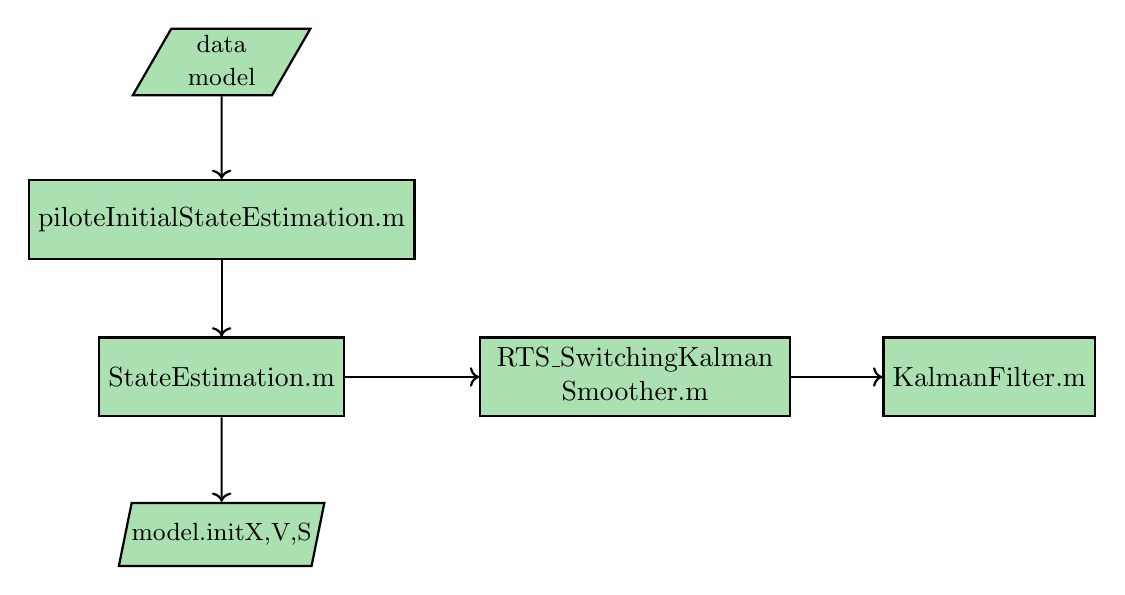
\begin{tikzpicture}

\node[paraceladon](inputHSE){\begin{tabular}{c}  \lstinline[ basicstyle = \mlttfamily \small]!data! \\ \lstinline[ basicstyle = \mlttfamily \small]!model! \end{tabular}};
\node[esceladon](piloteSE)[below of = inputHSE, yshift = -1cm]{\phantom{} piloteInitialStateEstimation.m \phantom{}};
\node[esceladon](SE)[below of = piloteSE, yshift = -1cm]{\phantom{} StateEstimation.m \phantom{}};
\node[esceladon](RTS)[right of = SE, yshift = 0cm, xshift = 4.25cm]{\begin{tabular}{c} RTS\_SwitchingKalman \\ Smoother.m \end{tabular}};
\node[esceladon](KF)[right of = RTS, yshift = 0cm, xshift = 3.5cm]{\phantom{} KalmanFilter.m \phantom{}};
\node[paraceladon](outputHSE)[below of = inputHSE, yshift = -5cm]{\lstinline[ basicstyle = \mlttfamily \small]!model.initX,V,S!};
%
\path[->, draw, thick] (inputHSE)edge(piloteSE);
\path[->, draw, thick] (piloteSE)edge(SE);
\path[->, draw, thick] (SE)edge(RTS);
\path[->, draw, thick] (RTS)edge(KF);
\path[->, draw, thick] (SE)edge(outputHSE);
\end{tikzpicture} } 
\caption{Initial hidden states estimation workflow} \label{FIG:InitialHiddenStateEstimationWorkflow}
\end{figure}



\section{Generate synthetic data}
\label{S:SYNTHETIC}
The creation of synthetic data is possible using OpenBDLM.
The analysis of synthetic data is useful for validation, test and debugging purposes because the true value of the hidden states and model parameters are known.
OpenBDLM uses the transition model  of the state-space modelling approach (see Section~\ref{SS:LGSSM}) to create realistic synthetic data.
There are two ways for creating synthetic data using OpenBDLM:

\begin{itemize}
\item From the interactive tool
\item From an existing project.
\end{itemize}

\subsection{Generate synthetic data using the interactive tool}
The creation of the synthetic data from the interactive tool (option \colorbox{light-gray}{\lstinline[basicstyle = \mlttfamily \small, backgroundcolor = \color{light-gray}]!0!} from the starting menu) enables to create synthetic data from scratch. 
OpenBDLM requests the user to provide the number of time series, and to define the time vector (starting time, end time, timestep).
In the next step, the user has to define the time-series dependence (if applicable), to provide the number of model class, and to choose the block component for each time-series, as well as model constrains between model classes (if applicable).
Default values for initial hidden states mean values and model parameters are automatically assigned for each block component.
In the case of two model classes, the synthetic baseline will switch between the first and the second model class according to the transition probability values (see Section~\ref{SS:THSKF}).
The amplitude of each synthetic anomaly (i.e. change of the local trend) is sampled randomly in a normal distribution of zero mean and standard deviation $\sigma_{w}^{12}$ as defined in the switching process noise transition matrix.
Alternatly, the user may choose to create \emph{custom anomalies}.
In such case, the beginning (in sample index), duration (in number of samples) and amplitude (in change of the local trend) of each anomaly is user specified.
The information about custom anomaly are stored in the field \lstinline[basicstyle = \mlttfamily \small, backgroundcolor = \color{light-gray}]!custom_anomalies! of the structure variable \lstinline[basicstyle = \mlttfamily \small, backgroundcolor = \color{light-gray}]!misc!:
\begin{itemize}
\item \lstinline[basicstyle = \mlttfamily \small, backgroundcolor = \color{light-gray}]!misc.custom_anomalies.start_custom_anomalies!: this field stores a $1\times \mathtt{A}$ vector of integers, where $\mathtt{A}$ is the total number of synthetic anomaly. Each value indicates the sample index of the anomaly start.
\item \lstinline[basicstyle = \mlttfamily \small, backgroundcolor = \color{light-gray}]!misc.custom_anomalies.duration_custom_anomalies!: this field stores a $1\times \mathtt{A}$ vector of integers, where $\mathtt{A}$ is the total number of synthetic anomaly. Each value indicates the anomaly duration in number of samples.
\item \lstinline[basicstyle = \mlttfamily \small, backgroundcolor = \color{light-gray}]!misc.custom_anomalies.amplitude_custom_anomalies!: this field stores a $1\times \mathtt{A}$ vector of real number, where $\mathtt{A}$ is the total number of synthetic anomaly. Each value indicates the amplitude of the anomaly in change of the local trend.
\end{itemize}
The synthetic data are saved in \lstinline[basicstyle = \mlttfamily \small, backgroundcolor = \color{light-gray}]!DATA_*.mat! and \lstinline[basicstyle = \mlttfamily \small, backgroundcolor = \color{light-gray}]!*.csv! data files, and a \lstinline[basicstyle = \mlttfamily \small, backgroundcolor = \color{light-gray}]!PROJ_*.mat! project file is created that stores the information about the model (structure variable \lstinline[basicstyle = \mlttfamily \small, backgroundcolor = \color{light-gray}]!model!), and the true hidden states (see structure variable \lstinline[basicstyle = \mlttfamily \small, backgroundcolor = \color{light-gray}]!estimation.ref!).





\begin{table}[h]

     \begin{tabular}{|C{1cm}"C{3.25cm} |C{3.25cm}  |C{3.25cm} |N}\thickhline
        & $\bm{\theta}$ & $\bm{\mu}_{0}$ & diag$(\mathbf{\Sigma}_{0})$ &\\[25pt]\thickhline
    $\mathtt{LL}$   &  $\sigma_{w}^{\mathtt{LL}}=0$ &$[10]$ & $[0.1^{2}]$ &\\[25pt]\hline
    $\mathtt{LT}$    & $\sigma_{w}^{\mathtt{LT}}=10^{-7}$ &  $[10, -0.1\times10^{-2}]$ & $[0.1^{2}, 0.1^{2}]$ &\\[25pt]\hline
     $\mathtt{LA}$   & $\sigma_{w}^{\mathtt{LA}}=10^{-8}$  &  $[10, -0.1\times10^{-2} , -0.1\times10^{-5}]$ & $[0.1^{2}, 0.1^{2}, 0.1^{2}]$ &\\[25pt]\hline
     $\mathtt{P}$  &  $p=[365.24, 1, 182.62] $, $\sigma_{w}^{\mathtt{P}}=0$  &$[10, 10]$ & $[0.2^{2}, 0.2^{2}]$  &\\[25pt]\hline
     $\mathtt{KR}$  & $p=[365.24]$, $\ell=0.5$, $\sigma_{w,0}^{\mathtt{KR}}=\sigma_{w,1}^{\mathtt{KR}}=0$ &  $[$$-0.97$, $1.65$, $1.73$, $-1.91$ , $0.23$, $0.37$, $-2.89$, $-0.22$, $0.73$, $-1.83$$]$ & $[$$0.01^{2}$, $0.01^{2}$, $0.01^{2}$, $0.01^{2}$ , $0.01^{2}$, $0.01^{2}$, $0.01^{2}$, $0.01^{2}$, $0.01^{2}$, $0.01^{2}$$]$  &\\[25pt]\hline  
         $\mathtt{AR}$   &  $\phi^{\mathtt{AR}}=0.75$, $\sigma_{w}^{\mathtt{AR}}=0.01$  &$[0]$ & $[0.1^{2}]$ &\\[25pt]\thickhline
     \end{tabular}
     \caption{Default value of model parameters and initial hidden state $\bm{\mu}_{0}$ and $\mathbf{\Sigma}_{0}$ for synthetic data generation.} 
\label{table:defaultsynthetic}
\end{table}

\subsection{Generate synthetic data from an existing project}



Once a project is loaded, it is possible to create synthetic data from it (option \colorbox{light-gray}{\lstinline[basicstyle = \mlttfamily \small, backgroundcolor = \color{light-gray}]!16!} from the main menu (see Listing~\ref{LST:OpenBDLMMainMenu}).
The synthetic data time vector will be the same as the time vector in memory, and missing data will be replicated.
The model used to create the synthetic data will be the same as the model of the current project, including current initial hidden states as well as model parameters values.
The creation of synthetic data in this way is particularly useful to closely mimic real dataset.
The synthetic data are saved in \lstinline[basicstyle = \mlttfamily \small, backgroundcolor = \color{light-gray}]!DATA_new_*.mat! and \lstinline[basicstyle = \mlttfamily \small, backgroundcolor = \color{light-gray}]!*.csv! data files, and a \lstinline[basicstyle = \mlttfamily \small, backgroundcolor = \color{light-gray}]!PROJ_new_*.mat! new project file is created that stores the information about the model (structure variable \lstinline[basicstyle = \mlttfamily \small, backgroundcolor = \color{light-gray}]!model!), and the true hidden states (see structure variable \lstinline[basicstyle = \mlttfamily \small, backgroundcolor = \color{light-gray}]!estimation.ref!).






\subsection{Synthetic data generation functions}


The synthetic data creation workflow is presented Figure~\ref{FIG:SyntheticDataCreationWorkflow}. 
The OpenBLDM functions used for synthetic data creation are:

\begin{description}[style=unboxed]

\item[Pilot function for synthetic data creation] \leavevmode
  \begin{lstlisting}[ basicstyle = \mlttfamily \small, breaklines=true]
[data,model,estimation,misc]=piloteSimulateData(data,model,estimation,misc)
  \end{lstlisting}

\item[Creates synthetic data] \leavevmode
  \begin{lstlisting}[ basicstyle = \mlttfamily \small, breaklines=true]
[data,model,estimation,misc]=SimulateData(data,model,misc,varargin)
  \end{lstlisting}

\item[Create synthetic data from transition probabilities] \leavevmode
  \begin{lstlisting}[ basicstyle = \mlttfamily \small, breaklines=true]
[data, model, estimation, misc]=simulateDataFromTransitionProbabilities(data,model,misc)
  \end{lstlisting}

\item[Create synthetic data from custom anomalies (for two model classes only)] \leavevmode
  \begin{lstlisting}[ basicstyle = \mlttfamily \small, breaklines=true]
[data,model,estimation,misc]=simulateDataFromCustomAnomalies(data,model,misc)
  \end{lstlisting}

  \item[Models configuration for synthetic data (for synthetic data creation from interactive tool only)] \leavevmode
  \begin{lstlisting}[ basicstyle = \mlttfamily \small, breaklines=true]
[data,model,estimation,misc]=configureModelForDataSimulation(data,model,estimation,misc)
 \end{lstlisting}
 
 \item[Requests user inputs to define the number of synthetic time series to create (for synthetic data creation from interactive tool only)] \leavevmode
  \begin{lstlisting}[ basicstyle = \mlttfamily \small, breaklines=true]
  [data,misc]=defineDataLabels(data,misc)
 \end{lstlisting}
 
\item[Requests user inputs to define synthetic data time vector (for synthetic data creation from interactive tool only)] \leavevmode
  \begin{lstlisting}[ basicstyle = \mlttfamily \small, breaklines=true]
[data,misc]=defineTimestamps(data,misc)
 \end{lstlisting}

\end{description}



\begin{figure}[h]
  \centering
  \captionsetup{justification=centering}
\scalebox{0.8}{
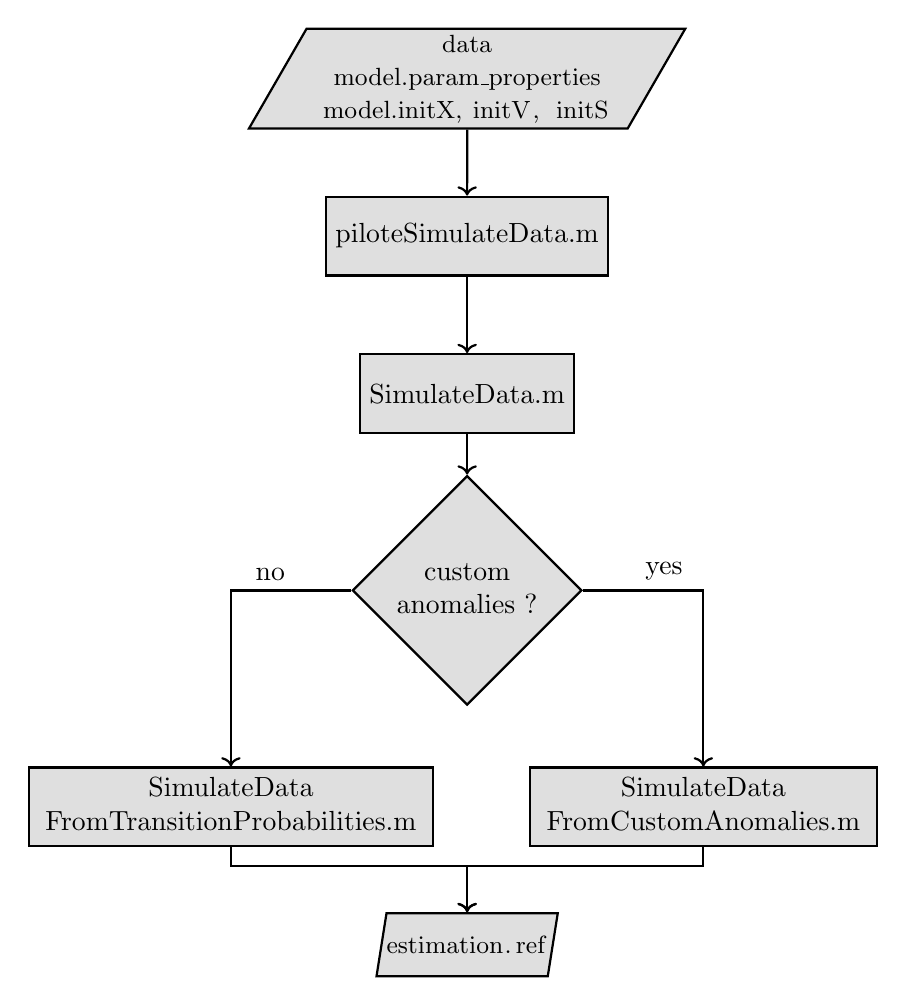
\begin{tikzpicture}

\node[paralightgray](inputSDC){\begin{tabular}{c}  \lstinline[ basicstyle = \mlttfamily \small]!data! \\ \lstinline[ basicstyle = \mlttfamily \small]!model.param_properties! \\ \lstinline[ basicstyle = \mlttfamily \small]!model.initX, initV, initS! \end{tabular}};
\node[eslightgray](piloteSDC)[below of = inputSDC, yshift = -1cm]{\phantom{} piloteSimulateData.m \phantom{}};
\node[eslightgray](SDC)[below of = piloteSDC, yshift = -1cm]{\phantom{} SimulateData.m \phantom{}};
\node[testlightgray](testCustom)[below of = SDC, yshift = -1.5cm]{\begin{tabular}{c}  custom  \\ anomalies ?  \end{tabular}};
\node[eslightgray](SDCtransition)[below of = testCustom, yshift = -1.75cm, xshift = -3cm]{\begin{tabular}{c} SimulateData \\ FromTransitionProbabilities.m \end{tabular}};
\node[eslightgray](SDCcustom)[below of = testCustom , yshift = -1.75cm, xshift = 3cm]{\begin{tabular}{c} SimulateData \\ FromCustomAnomalies.m \end{tabular}};
\node[paralightgray](outputSDC)[below of = inputSDC, yshift = -10cm]{\lstinline[ basicstyle = \mlttfamily \small]!estimation.ref!};
%
\path[->, draw, thick] (inputSDC)edge(piloteSDC);
\path[->, draw, thick] (piloteSDC)edge(SDC);
\path[->, draw, thick] (SDC)edge(testCustom);
\path[->, draw, thick] (testCustom.east) -| (2cm,-6.5cm) -| node[pos=0.25, above]{yes} (SDCcustom);
\path[->, draw, thick] (testCustom.west) -| (-2cm,-6.5cm) -| node[pos=0.25, above]{no} (SDCtransition);
\path[->, draw, thick] (SDCtransition.south) |- (0cm,-10cm) -|  (outputSDC.north);
\path[->, draw, thick] (SDCcustom.south) |- (0cm,-10cm) -|  (outputSDC.north);
\end{tikzpicture} } 
\caption{Synthetic data creation workflow} \label{FIG:SyntheticDataCreationWorkflow}
\end{figure}

\section{Results}

\subsection{Visualizing results}
\label{S:VisualizingResults}

The figures that popup on screen aim to represent the data, the data summary, and the hidden states results for each step of the analysis.
Note that in contrast with the data plot, the data summary plot offers a way  to visualize the amplitude, the timesteps and the data availability in a compact way.
By default, a solid line connects two successive real-valued measurement, whatever the timestep.
Missing data (NaN) are not represented in the plot of the observed data, thus resulting in gap for large period  of time with missing data.
The data availability in the data summary plot indicates each missing data with a red cross, thus making it useful to detect sparse missing data which are invisible in the data amplitude plots.
The working period of the sensor is represented by a thick green line in the data availability plot.
The plot appearance may be controlled from the dedicated \lstinline[basicstyle = \mlttfamily \small]!misc.options!.

\subsubsection{Generating figures at any time}
The option \colorbox{light-gray}{\lstinline[basicstyle = \mlttfamily \small]!14!} from the main menu allows generating the different type of figure at any time (see~\ref{LST:PlotMenu}).

\subsubsection{Saving figures}
It is not advised to save figures ``manually'' using the Matlab.
It would most likely not save figures as seen on the screen.
Instead, use the OpenBDLM export facilities described in the Section~\ref{SS:ExportResults}, or set the \lstinline[basicstyle = \mlttfamily \small]!misc.options.isExportTEX!, \lstinline[basicstyle = \mlttfamily \small]!misc.options.isExportPDF!, \lstinline[basicstyle = \mlttfamily \small]!misc.options.isExportPDF! to \lstinline[basicstyle = \mlttfamily \small]!true! to automatically save the figure in a specific format each time a figure is created \footnote{Automatic figure saving is not recommanded because it is computationally expensive.}.
The workflow for visualization is shown in Figure~\ref{FIG:ResultsVisualizationsWorkflow}. 
The functions used to visualize the data and results are:

\begin{lstlisting}[ frame = single, basicstyle = \mlttfamily \small, caption = {OpenBDLM plot menu}, label = LST:PlotMenu ,  float =ht, linewidth=\linewidth, captionpos=b]
----------------------------
/    Plot
----------------------------

     1 ->  Plot data 
     2 ->  Plot data summary 
     3 ->  Plot hidden states 

     Type R to return to the previous menu

     choice >> 
\end{lstlisting}



\begin{description}[style=unboxed]
\item[Pilote function to plot data and estimations] \leavevmode
  \begin{lstlisting}[ basicstyle = \mlttfamily \small, breaklines=true]
  [misc] = pilotePlot(data,model,estimation,misc)
 \end{lstlisting}

\item[Plot data amplitude values and data timestep] \leavevmode
  \begin{lstlisting}[ basicstyle = \mlttfamily \small, breaklines=true]
[FigureNames] = plotData(data,misc,varargin)
 \end{lstlisting}

\item[Plot data amplitude, data time step, and data availability ]  \leavevmode
  \begin{lstlisting}[ basicstyle = \mlttfamily \small, breaklines=true]
  plotDataSummary(data, misc, varargin)
 \end{lstlisting}

 \item[Plot hidden states, predicted data, and model probability]  \leavevmode
  \begin{lstlisting}[ basicstyle = \mlttfamily \small, breaklines=true]
plotEstimations(data,model,estimation,misc,varargin)
 \end{lstlisting}
 
  \item[Plot true and estimated hidden states]  \leavevmode
  \begin{lstlisting}[ basicstyle = \mlttfamily \small, breaklines=true]
  [FigureNames] = plotHiddenStates(data,model,estimation,misc,varargin)
 \end{lstlisting}
 
   \item[Plot observed and predicted data]  \leavevmode
  \begin{lstlisting}[ basicstyle = \mlttfamily \small, breaklines=true]
  [FigureNames] = plotPredictedData(data,model,estimation,misc,varargin)
 \end{lstlisting}
 
    \item[Plot true and estimated model probability]  \leavevmode
  \begin{lstlisting}[ basicstyle = \mlttfamily \small, breaklines=true]
  [FigureNames] = plotModelProbability(data,model,estimation,misc,varargin)
 \end{lstlisting}
 
     \item[Waterfall plot for kernel regression component]  \leavevmode
  \begin{lstlisting}[ basicstyle = \mlttfamily \small, breaklines=true]
[FigureNames] = plotWaterfallKRegression(data,model,estimation,misc,varargin)
 \end{lstlisting}
 
 \item[Export the current figure in TeX (tikz) file using matlab2tikz]  \leavevmode
  \begin{lstlisting}[ basicstyle = \mlttfamily \small, breaklines=true]
 exportPlot(FigureName,varargin)
 \end{lstlisting}
 
\end{description}


\begin{figure}[!h]
  \centering
  \captionsetup{justification=centering}
\scalebox{0.8}{
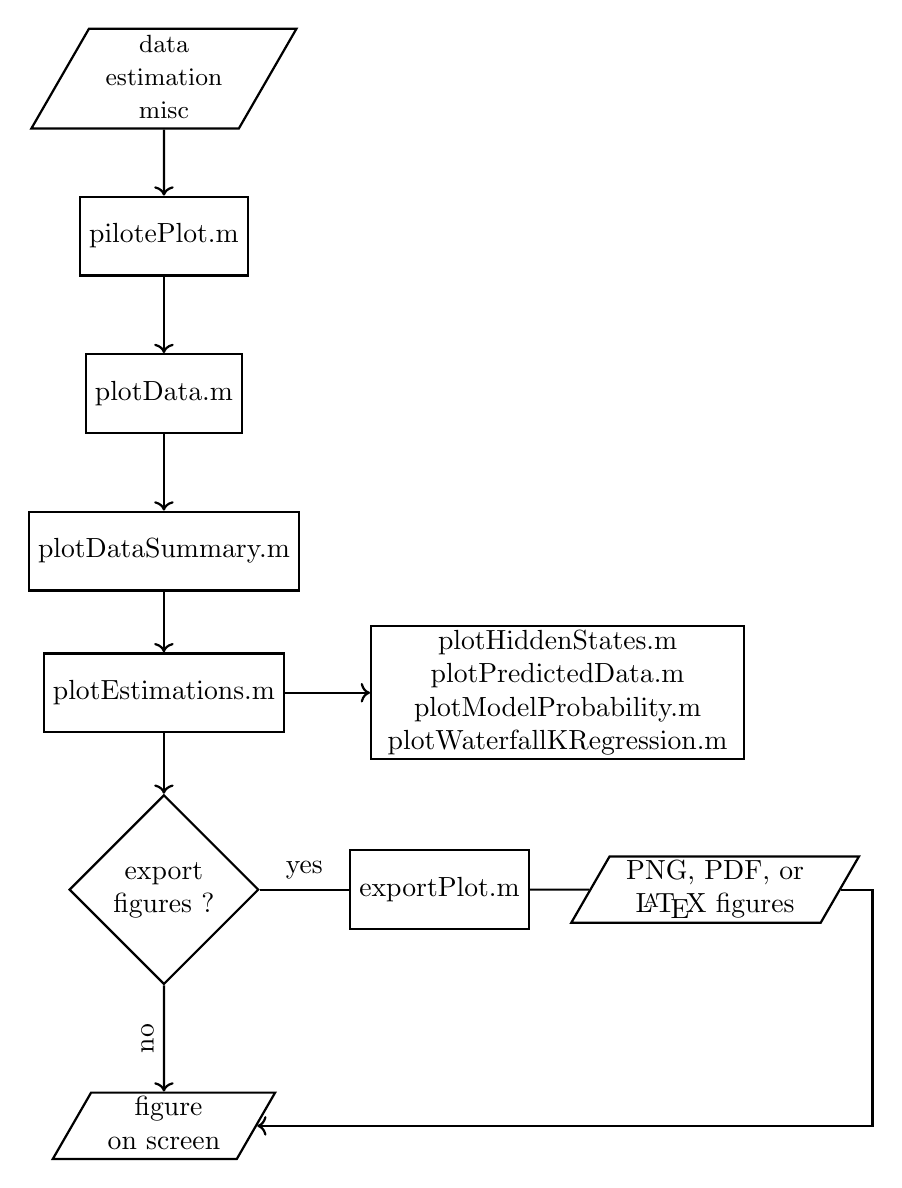
\begin{tikzpicture}

\node[parawhite](inputResultsVisualization){\begin{tabular}{c} \lstinline[basicstyle = \mlttfamily \small ]!data!  \\ \lstinline[basicstyle = \mlttfamily \small ]!estimation! \\ \lstinline[basicstyle = \mlttfamily \small ]!misc!  \end{tabular}};
\node[eswhite](pilote)[below of = inputResultsVisualization, yshift=-1cm, xshift = 0cm]{ \phantom{} pilotePlot.m \phantom{} };
\node[eswhite](plotData)[below of = pilote, yshift=-1cm, xshift = 0cm]{ \phantom{} plotData.m \phantom{} };
\node[eswhite](plotDataSummary)[below of = plotData, xshift = 0cm, yshift=-1cm, ]{ \phantom{} plotDataSummary.m \phantom{} };
\node[eswhite](plotEstimations)[below of = plotDataSummary, yshift= -0.8cm]{\phantom{} plotEstimations.m \phantom{}};
\node[eswhite](plotAll)[right of = plotEstimations, yshift= 0cm, xshift = 4cm]{\begin{tabular}{c} plotHiddenStates.m \\ plotPredictedData.m \\ plotModelProbability.m \\ plotWaterfallKRegression.m  \end{tabular}};
\node[testwhite](testExport)[below of = plotEstimations, yshift= -1.5cm, xshift = 0cm]{\begin{tabular}{c} export \\ figures ?  \end{tabular}};
\node[eswhite](Export)[right of = testExport , yshift=0cm, xshift = 2.5cm]{ \phantom{}  exportPlot.m \phantom{} };
\node[parawhite](outputExport)[right of = Export , yshift=0cm, xshift = 2.5cm]{ \begin{tabular}{c} PNG, PDF, or \\ \LaTeX{} figures \end{tabular}};
\node[parawhite](outputResultsVisualization1)[below of =testExport, yshift=-2cm, xshift = 0cm]{\begin{tabular}{c}  \MATLAB{} figure \\ on screen  \end{tabular}};

\path[->, thick] (inputResultsVisualization)edge(pilote);
\path[->, thick] (pilote)edge(plotData);
\path[->, thick] (plotData)edge(plotDataSummary);
\path[->, thick] (plotDataSummary)edge(plotEstimations);
\path[->, thick] (plotEstimations)edge(plotAll);
\path[->, thick] (plotEstimations)edge(testExport);
\path[-, thick] (testExport)edge  node[anchor=center, above, rotate=0, rotate=0]{ yes}  (Export);
\path[-, thick] (Export)edge(outputExport);
\path[->, thick] (testExport)edge node[anchor=center, above, rotate=0, rotate=90]{ no}  (outputResultsVisualization1);
\path[->, draw,  thick] (outputExport.east) -| (9cm, -12.95cm) |- (outputResultsVisualization1.east);

\end{tikzpicture} } 
\caption{Visualization results workflow} \label{FIG:ResultsVisualizationsWorkflow}
\end{figure}


\subsection{Exploring results}
\label{S:ExploringResults}

Exploring results (raw data and figures), is essential for interpretation, validation and reporting during and after the analysis.
During the analysis, the \MATLAB{} binary RES\_*.mat, PROJ\_*.mat and DATA\_*.mat files are automatically created for this purpose.
Moreover, OpenBDLM enables exporting results in user's specified format using the export menu (option \colorbox{light-gray}{\lstinline[basicstyle = \mlttfamily \small]!17!} from the main menu).
For instance, the results can be exported in CSV format for direct use in a third party software.
The figures can be exported in PDF, PNG, and \LaTeX{} (tikz) to create publication-quality figures.

\subsubsection{RES\_*.mat result file}

The \lstinline[basicstyle = \mlttfamily \small]!RES_*.mat! results file are located in the ``results/mat'' subfolder.
The \MATLAB{} binary .MAT contain four \MATLAB{} variables called  \lstinline[basicstyle = \mlttfamily \small]!timestamps!, \lstinline[basicstyle = \mlttfamily \small]!Mean!, \lstinline[basicstyle = \mlttfamily \small]!StandardDeviation!, and  \lstinline[basicstyle = \mlttfamily \small]!labels!.
\begin{itemize}
\item \lstinline[basicstyle = \mlttfamily \small]!timestamps!: $\mathtt{N}\times 1$ array containing the time vector.
\item \lstinline[basicstyle = \mlttfamily \small]!Mean!: $\mathtt{N}\times (\mathtt{L}+\mathtt{D}+1)$ array containing the filtered or smoothed posterior mean values of the hidden states, where $\mathtt{L}$ is the number of hidden states,  $\mathtt{D}$ is the number of time series.
\item \lstinline[basicstyle = \mlttfamily \small]!StandardDeviation!: $\mathtt{N}\times (\mathtt{L}+\mathtt{D}+1)$ array containing the filtered or smoothed posterior standard deviation values of the hidden states.
\item \lstinline[basicstyle = \mlttfamily \small]!labels!: $1\times (\mathtt{L}+\mathtt{D}+1)$ cell array containing the label of each column of the \lstinline[basicstyle = \mlttfamily \small]!Mean! and \lstinline[basicstyle = \mlttfamily \small]!StandardDeviation! arrays.
\end{itemize}

The function used to save the result is:

\begin{description}[style=unboxed]
\item[Save results in a .mat file] \leavevmode
  \begin{lstlisting}[ basicstyle = \mlttfamily \small, breaklines=true]
[misc]=saveResultsMAT(data,model,estimation,misc,varargin)
 \end{lstlisting}
\end{description}

\subsubsection{PROJ\_*.mat project file}

The \lstinline[basicstyle = \mlttfamily \small]!PROJ_*.mat! project file are located in the ``saved\_projects/mat'' subfolder.
This files  contains the internal variables \lstinline[basicstyle = \mlttfamily \small ]!model!,\lstinline[basicstyle = \mlttfamily \small ]!estimation!, \lstinline[basicstyle = \mlttfamily \small ]!misc!.
The  content of those internal variables is described in Section~\ref{S:OpenBDLMINPUTOUTPUT}.
The function used to save the project is:
\begin{description}[style=unboxed]
\item[Save the variables model, estimation, misc in a .mat project file] \leavevmode
  \begin{lstlisting}[ basicstyle = \mlttfamily \small, breaklines=true]
saveProject(model, estimation,misc,varargin)
 \end{lstlisting}
\end{description}

\subsubsection{DATA\_*.mat data file}

The \lstinline[basicstyle = \mlttfamily \small]!DATA_*.mat! data file are located in the ``data/mat'' subfolder.
This file contains three variables called \lstinline[basicstyle = \mlttfamily \small]!labels!, \lstinline[basicstyle = \mlttfamily \small]!timestamps!, and \lstinline[basicstyle = \mlttfamily \small]!values! that fully describe the time series data.
The content of those variables is described in Section~\ref{SS:MATInput}.
The function used to save the data is:
\begin{description}[style=unboxed]
\item[Save data in a binary Matlab .mat file] \leavevmode
  \begin{lstlisting}[ basicstyle = \mlttfamily \small, breaklines=true]
[misc, dataFilename] = saveDataBinary(data,misc,varargin)
 \end{lstlisting}
\end{description}

\subsubsection{Exporting results}
\label{SS:ExportResults}

The option \colorbox{light-gray}{\lstinline[basicstyle = \mlttfamily \small]!17!} from the main menu offers a way to export the data, the results, the project and the figures in specific format (see~\ref{LST:ExportMenu}).
It is possible to export the figures in PDF, PNG\footnote{Yair Altman, 2011, export\_fig, \url{https://www.mathworks.com/matlabcentral/fileexchange/23629-export\_fig}} and \LaTeX{}\footnote{Nico Schl�mer,2013, matlab2tikz, \url{https://www.mathworks.com/matlabcentral/fileexchange/22022-matlab2tikz-matlab2tikz}},\footnote{All the time-series figures shown in this document have been created from \LaTeX{} (tikz) files output from OpenBDLM. Minor post-processing have been done on the \LaTeX{} file. Compilation using LuaLatex.}.
It is possible to export the results and the data in .CSV files.
OpenBDLM creates one three-columns CSV file for each posterior filtered or smoothed hidden states for each time series, as well as CSV files for the predicted data for each time series, and a CSV file for the model probability.
The first column gives the timestamp, the second column the mean, and the third column the standard deviation.
The first line of each file is the header, that gives the reference name of the time-series associated with the hidden states as well as the date of the first timestamp in the \textquotesingle YYYY-DD-MM-HH-MM-SS\textquotesingle{} format. 
It is also possible to export the project in a configuration file that respects the format described in Section~\ref{S:CFGFile}.

\begin{lstlisting}[ frame = single, basicstyle = \mlttfamily \small, caption = {OpenBDLM export menu}, label = LST:ExportMenu ,  float =ht, linewidth=\linewidth, captionpos=b]
----------------------------------
/    Export
----------------------------------

     1 ->  Export the project in a configuration file
     2 ->  Export data in CSV format
     3 ->  Export results in CSV format
     4 ->  Create and export figures 

     Type R to return to the previous menu

     choice >> 
\end{lstlisting}

The export workflow is shown in Figure~\ref{FIG:ExportWorkflow}, and the functions used to export the results are:
\begin{description}[style=unboxed]
\item[Pilote function to export data, estimations and project] \leavevmode
  \begin{lstlisting}[ basicstyle = \mlttfamily \small, breaklines=true]
[misc]=piloteExport(data,model,estimation,misc)
 \end{lstlisting}

\item[Create and print a configuration file from project] \leavevmode
  \begin{lstlisting}[ basicstyle = \mlttfamily \small, breaklines=true]
  [configFilename] = printConfigurationFile(data,model,estimation,misc,varargin)
 \end{lstlisting}

\item[ Save time series data in separate .csv files] \leavevmode
  \begin{lstlisting}[ basicstyle = \mlttfamily \small, breaklines=true]
[misc] = saveDataCSV(data,misc,varargin)
 \end{lstlisting}

\item[ Save results in .CSV files] \leavevmode
  \begin{lstlisting}[ basicstyle = \mlttfamily \small, breaklines=true]
[misc]=saveResultsCSV(data, model, estimation, misc, varargin)
 \end{lstlisting}

\end{description}


\begin{figure}[!h]
  \centering
  \captionsetup{justification=centering}
\scalebox{0.8}{
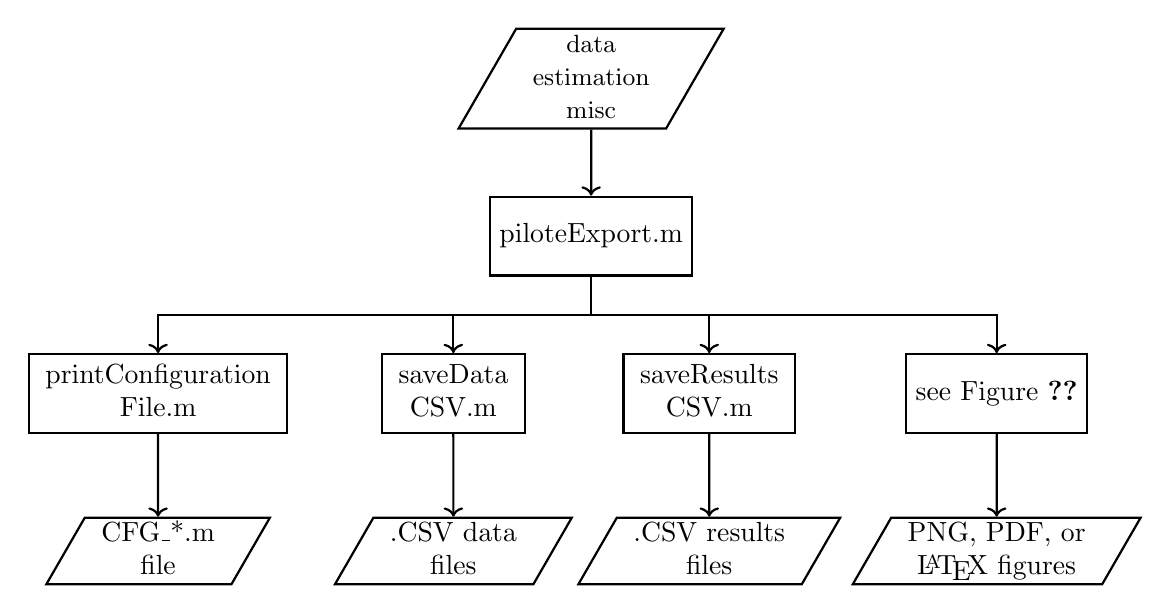
\begin{tikzpicture}

\node[parawhite](inputExport){\begin{tabular}{c} \lstinline[basicstyle = \mlttfamily \small ]!data!  \\ \lstinline[basicstyle = \mlttfamily \small ]!estimation! \\ \lstinline[basicstyle = \mlttfamily \small ]!misc!  \end{tabular}};
\node[eswhite](pilote)[below of = inputExport, yshift=-1cm, xshift = -0cm]{ \phantom{} piloteExport.m \phantom{} };
\node[eswhite](CFG)[below of = pilote, yshift=-1cm, xshift = -5.5cm]{\begin{tabular}{c} printConfiguration \\ File.m \end{tabular}};
\node[eswhite](DataCSV)[below of = pilote, yshift=-1cm, xshift = -1.75cm]{\begin{tabular}{c} saveData\\CSV.m   \end{tabular}};
\node[eswhite](ResultsCSV)[below of = pilote, yshift=-1cm, xshift = 1.5cm]{\begin{tabular}{c} saveResults\\CSV.m  \end{tabular} };
\node[eswhite](ExportFig)[below of = pilote, yshift=-1cm, xshift = 5.15cm]{ \phantom{} see Figure~\ref{FIG:ResultsVisualizationsWorkflow} \phantom{} };
\node[parawhite](outputCFG)[below of = CFG , yshift=-1cm, xshift = 0cm]{\begin{tabular}{c}  CFG\_*.m \\ file \end{tabular}};
\node[parawhite](outputDCSV)[below of = DataCSV , yshift=-1cm, xshift = 0cm]{\begin{tabular}{c} .CSV data \\ files \end{tabular}};
\node[parawhite](outputRCSV)[below of = ResultsCSV , yshift=-1cm, xshift = 0cm]{ \begin{tabular}{c} .CSV results \\ files \end{tabular}};
\node[parawhite](outputExport)[below of = ExportFig , yshift=-1cm, xshift = 0cm]{ \begin{tabular}{c} PNG, PDF, or \\ \LaTeX{} figures \end{tabular}};

\path[->, thick] (inputExport)edge(pilote);
\path[->, thick] (CFG)edge(outputCFG);
\path[->, thick] (DataCSV)edge(outputDCSV);
\path[->, thick] (ResultsCSV)edge(outputRCSV);
\path[->, thick] (ExportFig)edge(outputExport);
\path[->, draw,  thick] (pilote.south) |- (-4cm, -3cm) -| (CFG.north);
\path[->, draw,  thick] (pilote.south) |- (-2cm, -3cm) -| (DataCSV.north);
\path[->, draw,  thick] (pilote.south) |- (3cm, -3cm) -| (ResultsCSV.north);
\path[->, draw,  thick] (pilote.south) |- (5cm, -3cm) -| (ExportFig.north);

\end{tikzpicture} } 
\caption{Export options workflow} \label{FIG:ExportWorkflow}
\end{figure}









\input{section/OpenBDLMVersionControl}

\section{Examples}

\section{Step-by-step example: single time-series analysis}
\label{S:Example_DISP}

This example uses a single time series data that mimics displacement data measured on a bridge (synthetic data). 

\subsection{Step 1: start a project}

In the \MATLAB{} command window, type \colorbox{light-gray}{\lstinline[basicstyle = \mlttfamily \small, backgroundcolor = \color{light-gray}]!OpenBDLM_main;! }, and press the key ``enter'' $\dlsh$.
The \lstinline[basicstyle = \mlttfamily \small, backgroundcolor = \color{light-gray}]!OpenBDLM_main! starting menu appears.
The user has to provide an input from the command line each time a \lstinline[basicstyle = \mlttfamily \small, backgroundcolor = \color{light-gray}]!choice >>! appears.
%The provided input is validated by pressing $\dlsh$.
 \begin{lstlisting}[ frame = single, basicstyle = \mlttfamily \small, caption = {OpenBDLM command line interaction when calling \lstinline!OpenBDLM\_main;!} from \MATLAB{} command line, label = LST:OpenBDLMStartingMenuExample1 ,  float =h!, linewidth=\linewidth, captionpos=b]

------------------------------------------------
     Starting OpenBDLM_V1.0
------------------------------------------------
            Time series analysis using 
            Bayesian Dynamic Linear Models
------------------------------------------------
- Start a new project: 

     *      Enter a configuration filename 
     0   -> Interactive tool 

- Type D to Delete project(s), V for Version control, Q to Quit.

     choice >> 0
  
---------------------------------------
          Starting a new project...
----------------------------------------

- Enter a project name (max 25 characters):
     choice >> Example_DISP
     
- Does this project aim to create synthetic data ? (y/n) 
     choice >> no

     Load data...

- Choose a database

     0   -> Build a new database     	
 
     choice >> 0
\end{lstlisting}

First, choose the interactive tool by typing \colorbox{light-gray}{\lstinline[basicstyle = \mlttfamily \small, backgroundcolor = \color{light-gray}]!0!}.
Secondly, provide a project name (e.i \lstinline[basicstyle = \mlttfamily \small, backgroundcolor = \color{light-gray}]!Example_DISP!).
Then, answer \colorbox{light-gray}{\lstinline[basicstyle = \mlttfamily \small, backgroundcolor = \color{light-gray}]!no!} to indicate that you are not concerned with creating synthetic data.
The next step is to type \colorbox{light-gray}{\lstinline[basicstyle = \mlttfamily \small, backgroundcolor = \color{light-gray}]!0!} to indicate that you aim to load new data.

\subsection{Step 2: load the data}

At this stage, a graphical user interface \footnote{Douglas M. Schwarz, 2007, uipickfiles \url{https://www.mathworks.com/matlabcentral/fileexchange/10867-uipickfiles-uigetfile-on-steroids}} should appear on screen. 
Browse the ``examples/Example\_DISP'' folder to select the csv file named \lstinline[basicstyle = \mlttfamily \small, backgroundcolor = \color{light-gray}]!Example_DISP_DISP.csv!.
Then, click on the Add button, and then the Done button, as highlighted in Figure~\ref{fig:DataLoadingUIPickFileExample1}.
You will notice that some basic information regarding the loaded time-series, such as the time series index, the reference name and the number of data points are now displayed in the \MATLAB{} command window, as depicted in Listing~\ref{LST:OpenBDLMDataAvailabilityExample1}.
At this time, three \MATLAB{} figures as those represented in Figure~\ref{fig:DataSummary1} should popup on screen.
The first figure represents the data amplitude; the second figure represents the data timestep, and the last figure the data availability.
The figures show that data points exist between August 2013 and October 2015 (see Figure~\ref{fig:DataSummary1}a).
The timestep is non-uniform; it varies from 1 hour to 25 hours (see Figure~\ref{fig:DataSummary1}b). 
The most frequent (i.e referent) time step is 1 hour.
There is no missing data (see Figure~\ref{fig:DataSummary1}c).

\begin{figure*}[h!]
\begin{center}
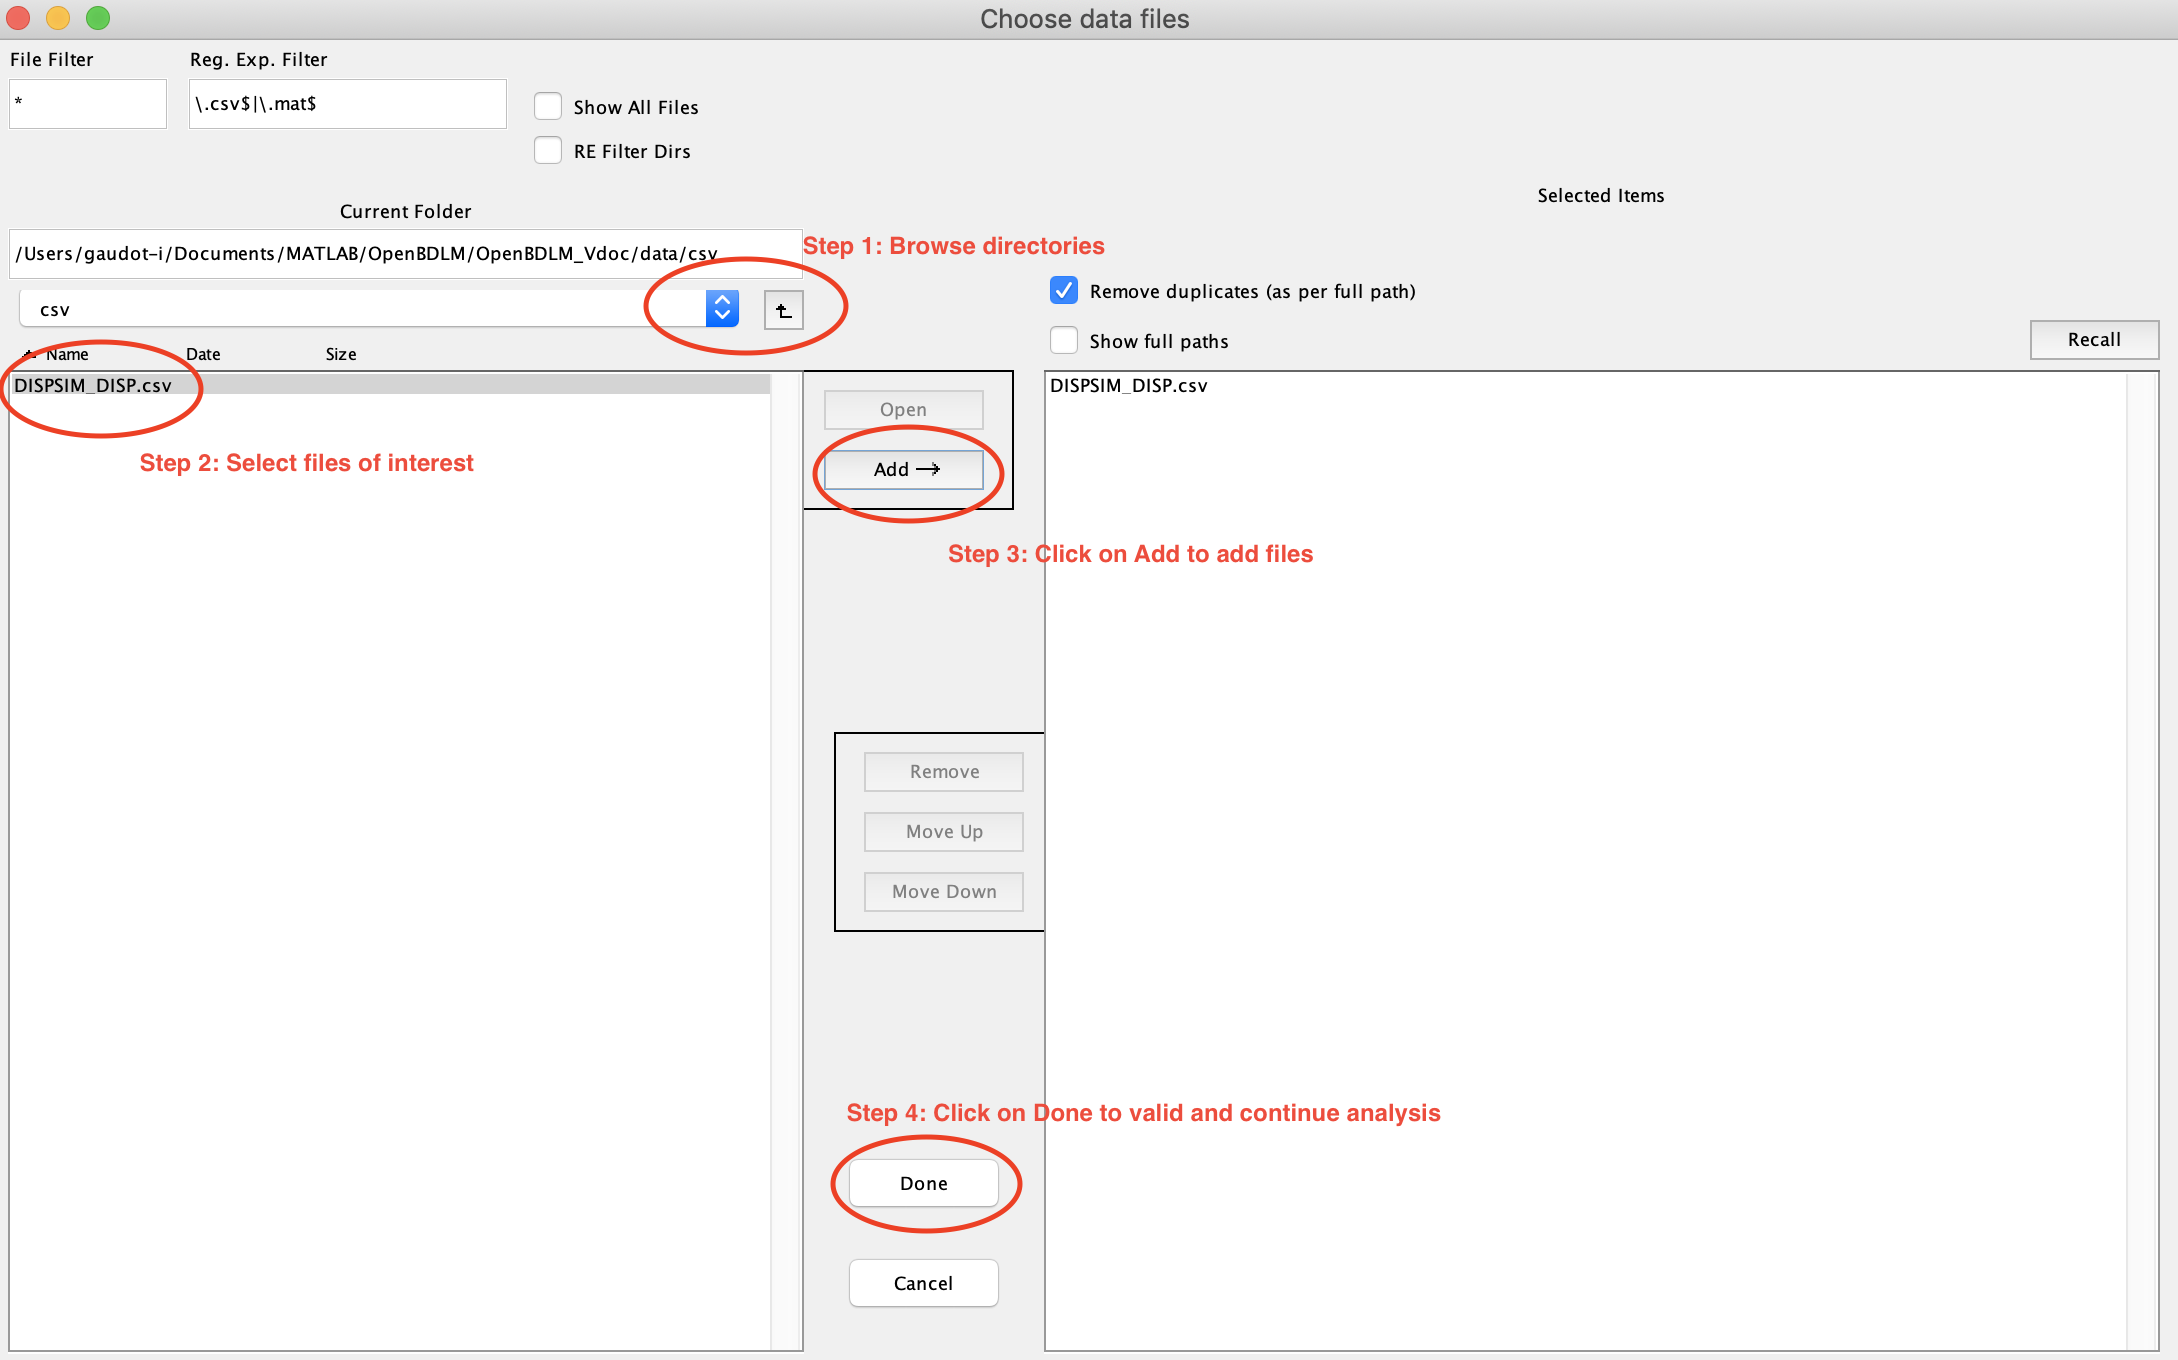
\includegraphics[width=0.9\linewidth]{./docfigs/Example_DISPSIM/dataloading_DISPSIM_uipickfiles_annoted.png}
\caption{Interactive data loading using the graphical user interface.}.
\label{fig:DataLoadingUIPickFileExample1}
\end{center}
\end{figure*}

 \begin{lstlisting}[ frame = single, basicstyle = \mlttfamily \small, caption = { \MATLAB{} command window output after the loading of a data file.}, label = LST:OpenBDLMDataAvailabilityExample1,  float =h!, linewidth=\linewidth, captionpos=b]
- Data available: 
 
     Time series number #      Reference name            Size                     	
     -----------------------------------------------------------------
     1                         DISP                      [19366x1]                	
     -----------------------------------------------------------------
\end{lstlisting}


\begin{figure*}[h!]
\centering
\begin{subfigure}{\linewidth}
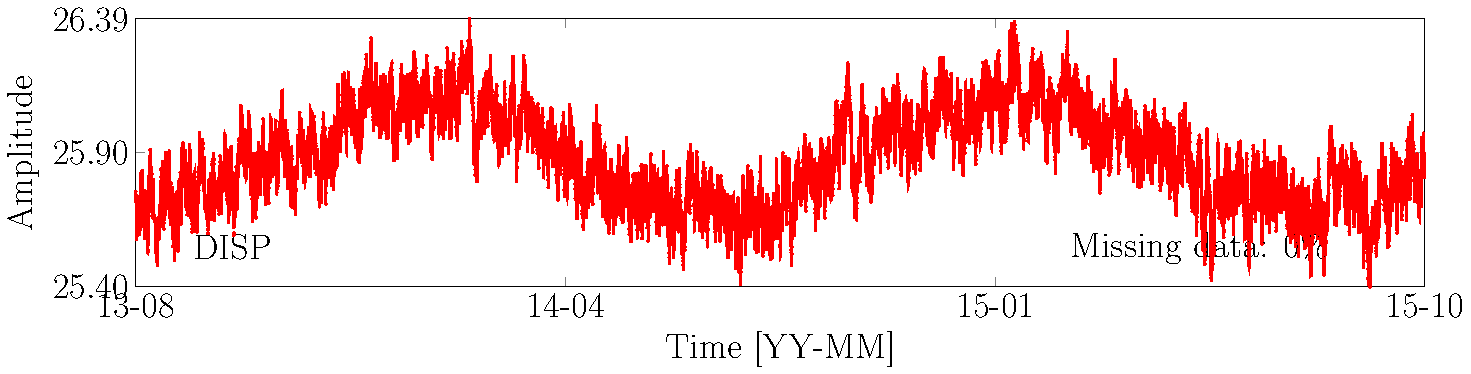
\includegraphics[width=0.9\linewidth]{./docfigs/Example_DISPSIM/raw/ALL_AMPLITUDES.pdf}
\caption{Amplitude}
\end{subfigure}
\begin{subfigure}{\linewidth}
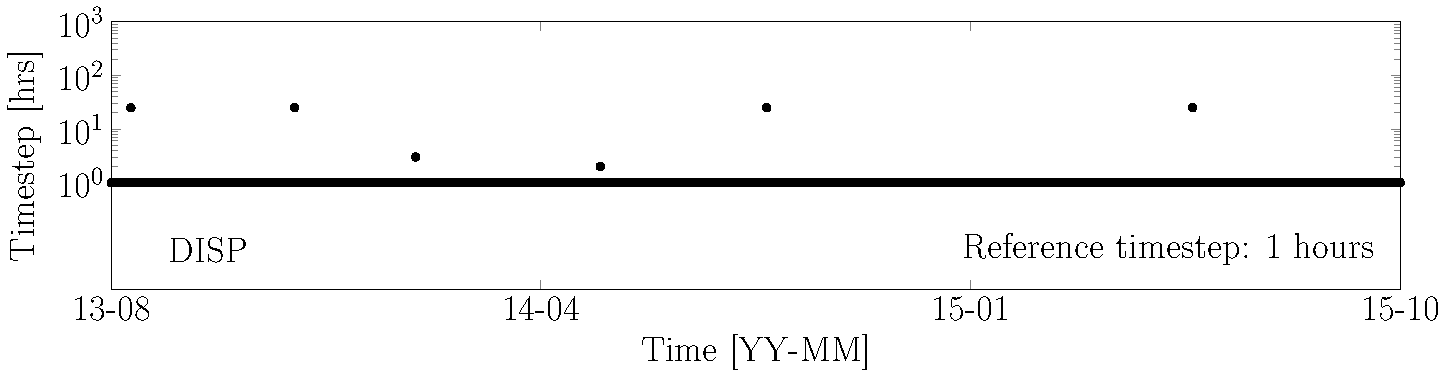
\includegraphics[width=0.9\linewidth]{./docfigs/Example_DISPSIM/raw/ALL_TIMESTEPS.pdf} 
\caption{Timestep}
\end{subfigure}
\begin{subfigure}{\linewidth}
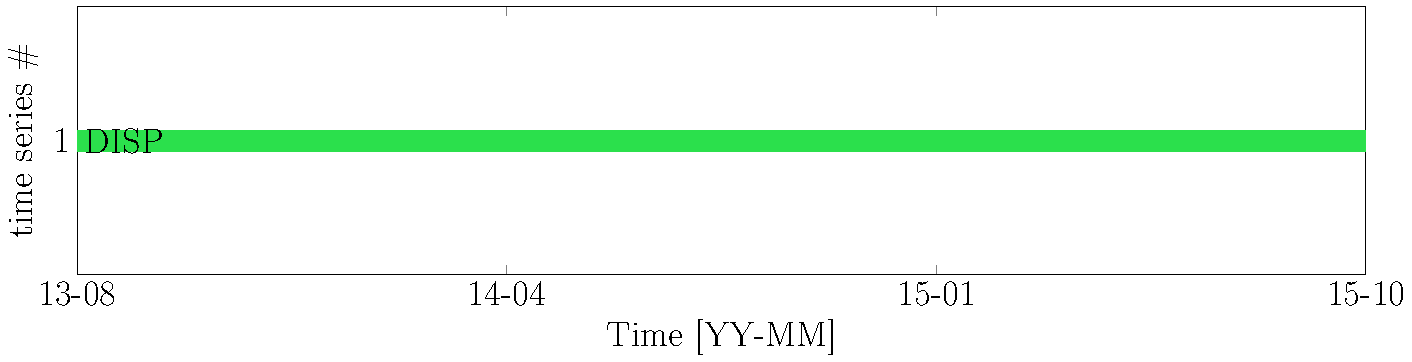
\includegraphics[width=0.9\linewidth]{./docfigs/Example_DISPSIM/raw/AVAILABILITY.pdf}
\caption{Availbility}
\end{subfigure}
\caption{Data used in the example presented Section~\ref{S:Example_DISP}.}
\label{fig:DataSummary1}
\end{figure*}

\subsection{Step 3: edit and pre-process the data}

The data editing and preprocessing menu as depicted in Listing~\ref{LST:Editing_menu} appear.
In this example, the objective is to use the data as such.
Therefore, no editing or preprocessing is done.
Therefore, type \colorbox{light-gray}{\lstinline[basicstyle = \mlttfamily \small, backgroundcolor = \color{light-gray}]!7!} to save the data as such, and continue analysis.

\subsection{Step 4: configure the model}

First, the program requests the number of model class.
In this example, the time series data looks stationary and we are not interested in anomaly detection, so type type \colorbox{light-gray}{\lstinline[basicstyle = \mlttfamily \small, backgroundcolor = \color{light-gray}]!1!}.
Secondly, OpenBDLM asks for the type of block component. 
Type \colorbox{light-gray}{\lstinline[basicstyle = \mlttfamily \small, backgroundcolor = \color{light-gray}]![11 31 31 41]!} to define a model with a local level, a yearly periodic component, a daily periodic component and an autoregressive component.
The  output on \MATLAB{} command window during interactive model configuration is presented in Listing~\ref{LST:OpenBDLMModelConfigureExample1}.
%Press the enter key $\dlsh$ to valid.
The model is then built, a {\lstinline[basicstyle = \mlttfamily \small, backgroundcolor = \color{light-gray}]!DATA_Example_DISP.mat!} binary data file, a {\lstinline[basicstyle = \mlttfamily \small, backgroundcolor = \color{light-gray}]!CFG_Example_DISP.m!} configuration file, as well as a {\lstinline[basicstyle = \mlttfamily \small, backgroundcolor = \color{light-gray}]!PROJ_Example_DISP.mat!} project file are created.
The OpenBLDM main menu must appear on the \MATLAB{} command window (see Listing~\ref{LST:OpenBDLMMainMenu}).
Type \colorbox{light-gray}{\lstinline[basicstyle = \mlttfamily \small, backgroundcolor = \color{light-gray}]!Q!} to save and quit.

 \begin{lstlisting}[ frame = single, basicstyle = \mlttfamily \small, caption = { \MATLAB{} command window output during interactive model configuration.}, label = LST:OpenBDLMModelConfigureExample1,  float =h, linewidth=\linewidth, captionpos=b]
- How many model classes do you want for each time-series? 
     choice >> 1
     
     --------------------------------------------------------
     BDLM Component reference numbers
     --------------------------------------------------------
     11: Local level 
     12: Local trend 
     13: Local acceleration 
     21: Local level compatible with local trend 
     22: Local level compatible with local acceleration 
     23: Local trend compatible with local acceleration 
     31: Periodic 
     41: Autoregressive process (AR(1)) 
     51: Kernel regression 
     61: Level Intervention 
     --------------------------------------------------------

- Identify components for time series #1; e.g. [11 31 41]
     choice >> [11 31 31 41]

     Building model...
     Saving project...
     Project saved in saved_projects/PROJ_Example_DISP.mat. 
     Printing configuration file...
     Saving data...

     Database saved in data/mat/DATA_Example_DISP.mat 
     Configuration file saved in config_files/CFG_Example_DISP.m. 

\end{lstlisting}


\subsection{Step 5: open the configuration file}

After the data loading and the model configuration, a configuration file named \lstinline[basicstyle = \mlttfamily \small, backgroundcolor = \color{light-gray}]!CFG_Example_DISP.csv! is automatically created and saved in ``config\_files'' folder.
Open the configuration file from \MATLAB{} command line by typing  \colorbox{light-gray}{\lstinline[basicstyle = \mlttfamily \small, backgroundcolor = \color{light-gray}]!edit CFG_Example_DISP.m!}.
The first part of this configuration file as it should appear on the \MATLAB{} editor is shown in Listing~\ref{LST:CFGFileExample1}.
The Model parameters section of the configuration file shows that the model totalizes 8 model parameters, that is 
\begin{gather*}
\bm\theta=\{\sigma_{w}^{LL}, p^{\text{PD1}}, \sigma_{w}^{\text{PD1}} , p^{\text{PD2}}, \sigma_{w}^{\text{PD2}}, \phi^{AR}, \sigma_{w}^{AR}, \sigma_{v}\}.
\end{gather*}
%The default value of the model parameters are assigned   using heuristic knowledge or computed from the data using statistics on the data.
The default model parameters values are 
\begin{gather*}
\bm\theta^{\text{default}}=\{0, 365.2422, 0, 1, 0, 0.75, 0.0174, 0.0087002 \}.
\end{gather*}
%In the same manner, default value for the initial hidden states are assigned using heuristic knowledge or computed using statistics on the data.
The default  hidden states mean  and covariance values are 
\begin{align*}
\bm \mu^{\text{default}}_{0} & = [25.8 , 5  ,   	0     ,	5   ,  	0    , 	0     ]^{\intercal}, \text{and} \\
 \text{diag}(\bm\Sigma^{\text{default}}_{0}) & = [	0.121 	,0.121 ,	0.121 ,	0.121 ,	0.121 	, 0.0303     ], 
 \end{align*}
 respectively.

\begin{lstlisting}[linewidth=\linewidth, style=Matlab-editor,  basicstyle = \mlttfamily \scriptsize, backgroundcolor = \color{matlab-yellow}, caption = {Example of a configuration file}, label=LST:CFGFileExample1, ,captionpos=b, float=h!]
%                    OpenBDLM configuration file                          
%          Autogenerated by OpenBDLM on 22-Nov-2018 17:18:09              
%
%% A - Project name
misc.ProjectName='Example_DISP';

%% B - Data
dat=load('DATA_Example_DISP.mat'); 
data.values=dat.values;
data.timestamps=dat.timestamps;
data.labels={'Example_DISP'};

%% C - Model structure 
% Components reference numbers
% 11: Local level
% 12: Local trend
% 13: Local acceleration
% 21: Local level compatible with local trend
% 22: Local level compatible with local acceleration
% 23: Local trend compatible with local acceleration
% 31: Periodic
% 41: Autoregressive
% 51: Kernel regression

% Model components
% Model 1
model.components.block{1}={[11 31 31 41] };

% Model component constrains | Take the same  parameter as model class #1
 
% Model inter-components dependence | {[components form dataset_i depends on components from  dataset_j]_i,[...]}
model.components.ic={[ ] };
%
%% D - Model parameters 
model.param_properties={
     % #1       #2       #3    #4    #5         #6       #7     #8     #9    #10
     % Param name Block name  Model Obs Bound Prior Mean Std Values Ref
     '\sigma_w', 'LL',  '1',   '1', [NaN  NaN],    'N/A',  NaN, NaN,  0,          1 %#1   
     'p',        'PD1', '1',   '1', [NaN  NaN],    'N/A',  NaN, NaN, 365.24,      2 %#2   
     '\sigma_w', 'PD1', '1',   '1', [NaN  NaN],    'N/A',  NaN, NaN,   0,         3 %#3   
     'p',        'PD2', '1',   '1', [NaN  NaN],    'N/A',  NaN, NaN,   1,         4 %#4   
     '\sigma_w', 'PD2', '1',   '1', [NaN  NaN],    'N/A',  NaN, NaN,   0,         5 %#5   
     '\phi',     'AR',  '1',   '1', [0  1],        'N/A',  NaN, NaN,   0.75,      6 %#6   
     '\sigma_w', 'AR',  '1',   '1', [0  Inf],      'N/A',  NaN, NaN,   0.0174,    7 %#7   
     '\sigma_v', '',    '1',   '1', [0  Inf],      'N/A',  NaN, NaN,   0.0087002, 8 %#8   
};

%% E - Initial states values 
% Initial hidden states mean for model 1:
model.initX{ 1 }=[	25.8  	5     	0     	5     	0     	0     ]';

% Initial hidden states variance for model 1: 
model.initV{ 1 }=diag([ 	0.121 	0.121 	0.121 	0.121 	0.121 	0.0303 ]);

% Initial probability for model 1
model.initS{1}=[1     ];

\end{lstlisting}

\subsection{Step 6: estimate the hidden states}

Type \colorbox{light-gray}{\lstinline[basicstyle = \mlttfamily \small, backgroundcolor = \color{light-gray}]!OpenBDLM_main('CFG_Example_DISP.m');!} in the \MATLAB{} command line.
Once, the main menu appears, type  \colorbox{light-gray}{\lstinline[basicstyle = \mlttfamily \small, backgroundcolor = \color{light-gray}]!3!}, then \colorbox{light-gray}{\lstinline[basicstyle = \mlttfamily \small, backgroundcolor = \color{light-gray}]!1!} to estimate the filtered hidden states using the default model parameters and default initial hidden states values.
The value of the log-likelihood is $36626$, and the estimated hidden states are presented in Figure~\ref{fig:Example_DISPSIMDefaultDefaultExample1}.

\begin{figure*}[h!]
\centering
\begin{subfigure}{\linewidth}
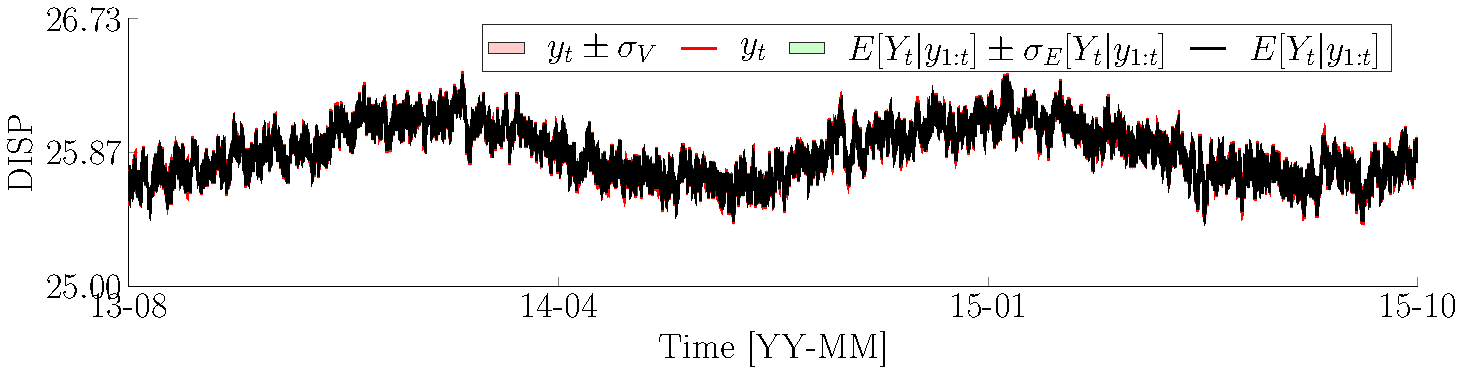
\includegraphics[width=0.9\linewidth]{./docfigs/Example_DISPSIM/default/DISP_ObservedPredicted.pdf} 
\caption{Observed and estimated displacement data}
\end{subfigure}
\begin{subfigure}{\linewidth}
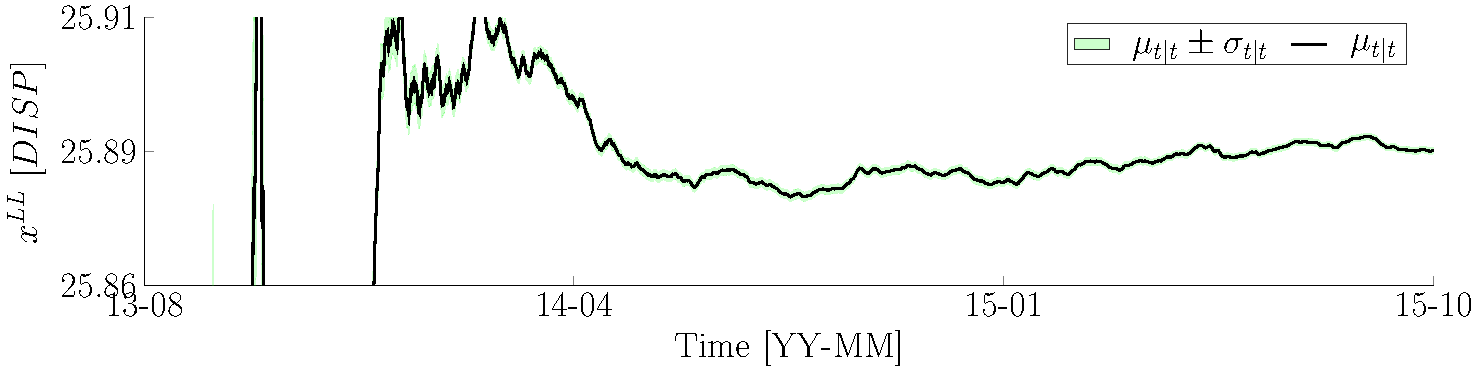
\includegraphics[width=0.9\linewidth]{./docfigs/Example_DISPSIM/default/DISP_LL_1.pdf}
\caption{Estimated displacement local level component}.
\end{subfigure}
\begin{subfigure}{\linewidth}
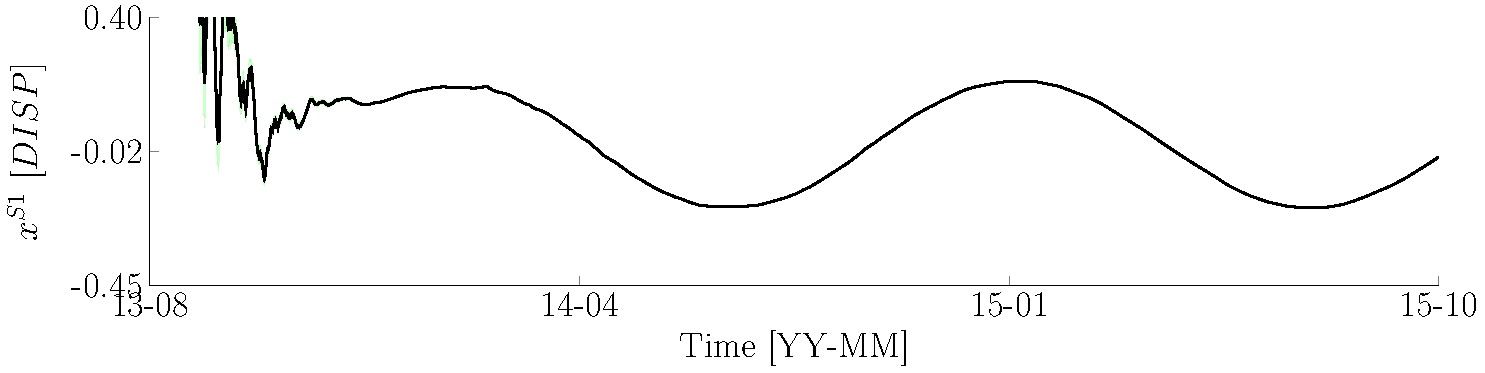
\includegraphics[width=0.9\linewidth]{./docfigs/Example_DISPSIM/default/DISP_S1_2.pdf}
\caption{Estimated displacement yearly periodic component}
\end{subfigure}
\begin{subfigure}{\linewidth}
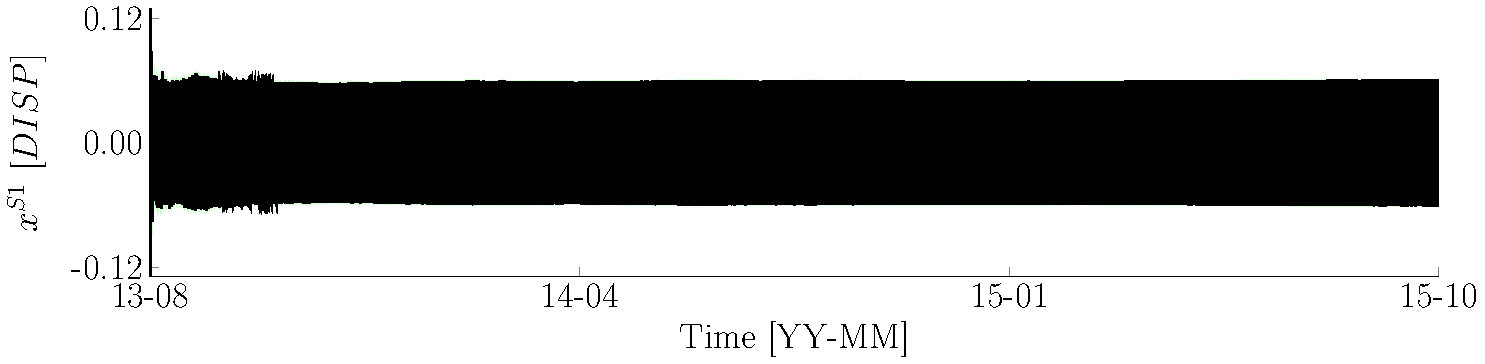
\includegraphics[width=0.9\linewidth]{./docfigs/Example_DISPSIM/default/DISP_S1_4.pdf}
\caption{Estimated displacement daily periodic component}
\end{subfigure}
\begin{subfigure}{\linewidth}
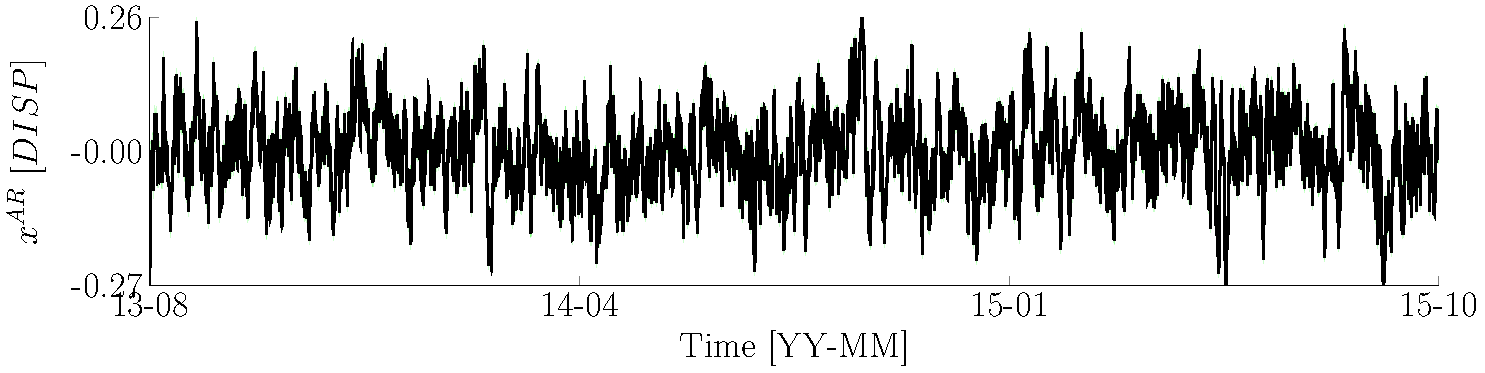
\includegraphics[width=0.9\linewidth]{./docfigs/Example_DISPSIM/default/DISP_AR_6.pdf} 
\caption{Estimated displacement autoregressive component}
\end{subfigure}
\caption{Estimated results using OpenBDLM defaults model parameters and default initial hidden states. The hidden states are estimated from the data presented in Figure~\ref{fig:DataSummary1}a. The solid line and shaded area represent the mean and standard deviation of the estimated hidden states, respectively.}
\label{fig:Example_DISPSIMDefaultDefaultExample1}
\end{figure*}

\subsection{Step 7: estimate the model parameters from the data}

Type \colorbox{light-gray}{\lstinline[basicstyle = \mlttfamily \small, backgroundcolor = \color{light-gray}]!OpenBDLM_main('CFG_Example_DISP.m');!} in the \MATLAB{} command line.
Once, the main menu appears, type  \colorbox{light-gray}{\lstinline[basicstyle = \mlttfamily \small, backgroundcolor = \color{light-gray}]!1!}, then \colorbox{light-gray}{\lstinline[basicstyle = \mlttfamily \small, backgroundcolor = \color{light-gray}]!1!} to estimate the model parameters using Newton-Raphson (type  \colorbox{light-gray}{\lstinline[basicstyle = \mlttfamily \small, backgroundcolor = \color{light-gray}]!2!} to use the Stochastic Gradient Descent instead).
The model parameters learning procedure starts, and messages are printed on \MATLAB{} command window to monitor the convergence through iterations (see Listing~\ref{LST:OpenBLDMModelParameterLearning}).
Note that, by default, OpenBDLM considers that the parameters $\sigma_{w}^{LL}$, $p^{\text{PD1}}$, $\sigma_{w}^{\text{PD1}}$ , $p^{\text{PD2}}$, $\sigma_{w}^{\text{PD2}}$ are known.
Therefore, there are three model parameters to be learned from the data in this example.
The estimation of the model parameters may take several hours.
Therefore, press combinations \colorbox{light-gray}{\lstinline[basicstyle = \mlttfamily \small, backgroundcolor = \color{light-gray}]!Ctrl!} + \colorbox{light-gray}{\lstinline[basicstyle = \mlttfamily \small, backgroundcolor = \color{light-gray}]!c!} to abort the process.
Once the algorithm is converged, the optimized model parameters values should be close to \footnote{Note that it is possible to get slightly different value of parameters with the same performance.}
\begin{gather*}
\bm\theta^{\text{*}}=\{0, 365.2422, 0, 1, 0, 0.97, 0.0192, 7.4258\times10^{-7} \}.
\end{gather*}

\subsection{Step 8: estimate the hidden states using the optimized model parameters values}

In the ``examples/Example\_DISP'' folder, there is a configuration file named \lstinline[basicstyle = \mlttfamily \small, backgroundcolor = \color{light-gray}]!CFG_Example_DISP_optim.m'! that contains optimized model parameters estimated using the Newton-Raphson algorithm.
Copy and paste \lstinline[basicstyle = \mlttfamily \small, backgroundcolor = \color{light-gray}]!CFG_Example_DISP_optim.m'! from  the ``examples/Example\_DISP'' subfolder  to the ``config\_files'' folder.
Type \colorbox{light-gray}{\lstinline[basicstyle = \mlttfamily \small, backgroundcolor = \color{light-gray}]!OpenBDLM_main('CFG_Example_DISP_optim.m');!} in the \MATLAB{} command line to load the configuration file  \lstinline[basicstyle = \mlttfamily \small, backgroundcolor = \color{light-gray}]!CFG_Example_DISP_optim.m!.
Once the main menu appears, type  \colorbox{light-gray}{\lstinline[basicstyle = \mlttfamily \small, backgroundcolor = \color{light-gray}]!3!}, then \colorbox{light-gray}{\lstinline[basicstyle = \mlttfamily \small, backgroundcolor = \color{light-gray}]!1!} to estimate the filtered hidden states using the optimized model parameters and default initial hidden states values.
The value of the log-likelihood is now $48819$.
The estimated hidden states are presented in Figure~\ref{fig:Example_DISPSIMOptimizedDefaultExample1}.

\begin{figure*}[h!]
\begin{center}
\begin{subfigure}{\linewidth}
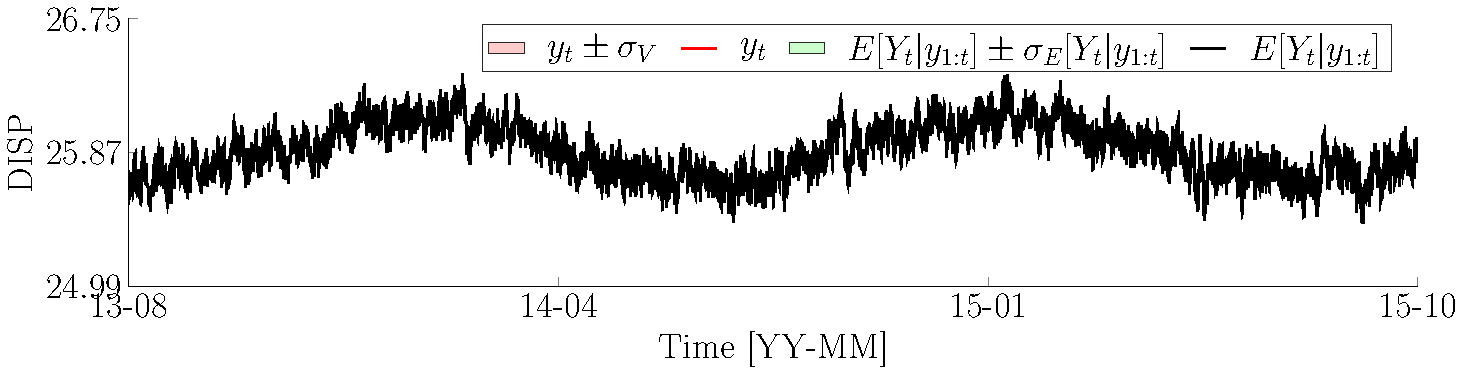
\includegraphics[width=0.9\linewidth]{./docfigs/Example_DISPSIM/optim_param_default_initialhiddenstate/DISP_ObservedPredicted.pdf}
\caption{Observed and estimated displacement data}
\end{subfigure}
\begin{subfigure}{\linewidth}
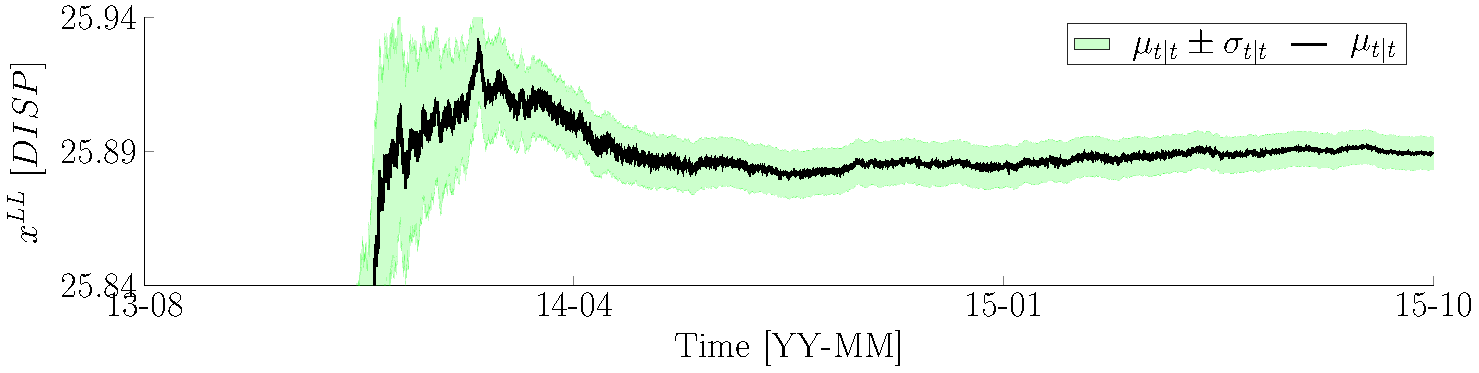
\includegraphics[width=0.9\linewidth]{./docfigs/Example_DISPSIM/optim_param_default_initialhiddenstate/DISP_LL_1.pdf}
\caption{Estimated displacement local level.}
\end{subfigure}
\begin{subfigure}{\linewidth}
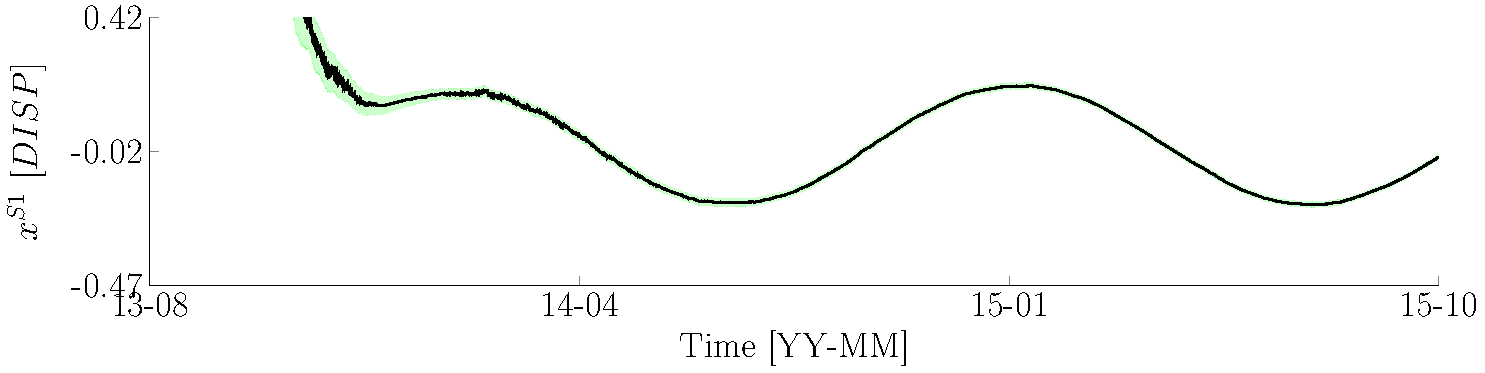
\includegraphics[width=0.9\linewidth]{./docfigs/Example_DISPSIM/optim_param_default_initialhiddenstate/DISP_S1_2.pdf}
\caption{Estimated displacement yearly periodic component (first hidden state)}
\end{subfigure}
\begin{subfigure}{\linewidth}
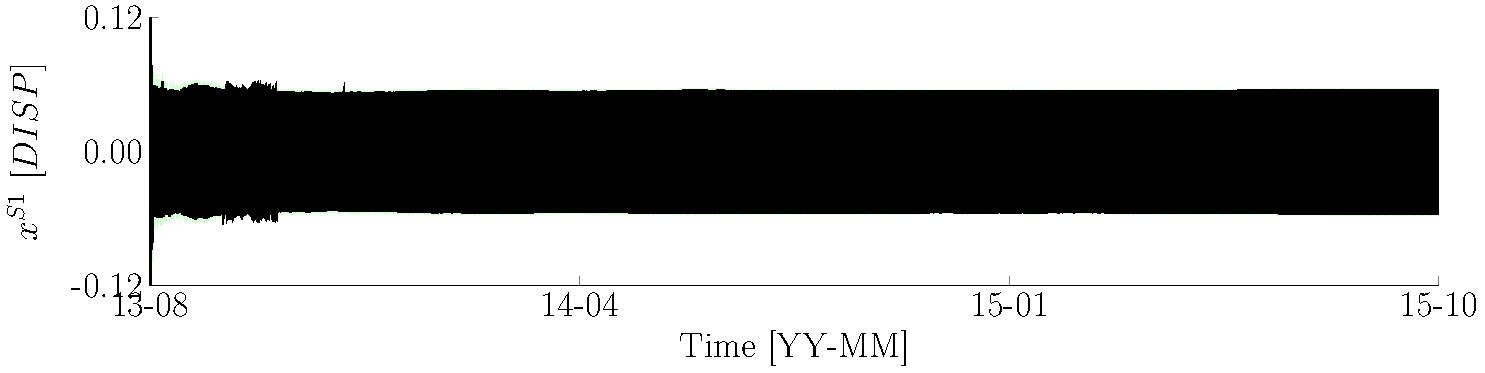
\includegraphics[width=0.9\linewidth]{./docfigs/Example_DISPSIM/optim_param_default_initialhiddenstate/DISP_S1_4.pdf} 
\caption{Estimated displacement daily periodic component (first hidden state)}
\end{subfigure}
\begin{subfigure}{\linewidth}
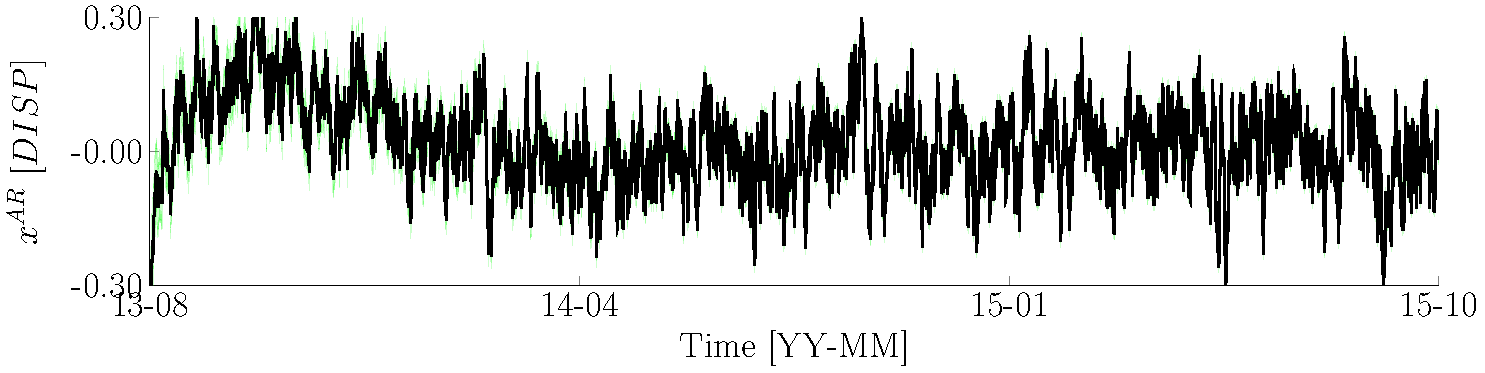
\includegraphics[width=0.9\linewidth]{./docfigs/Example_DISPSIM/optim_param_default_initialhiddenstate/DISP_AR_6.pdf} 
\caption{Estimated displacement autoregressive component}
\end{subfigure}
\caption{Estimated results using OpenBDLM optimized model parameters and default initial hidden states. The hidden states are estimated from the data presented in Figure~\ref{fig:DataSummary1}a. The solid line and shaded area represent the mean and standard deviation of the estimated hidden states, respectively.}
\label{fig:Example_DISPSIMOptimizedDefaultExample1}
\end{center}
\end{figure*}

\subsection{Step 9: estimate the initial hidden states}

Type \colorbox{light-gray}{\lstinline[basicstyle = \mlttfamily \small, backgroundcolor = \color{light-gray}]!OpenBDLM_main('CFG_Example_DISP_optim.m');!} in the \MATLAB{} command line.
Then, type  \colorbox{light-gray}{\lstinline[basicstyle = \mlttfamily \small, backgroundcolor = \color{light-gray}]!2!}, to optimize the initial hidden states value.
The estimated initial hidden states mean and covariance values are 
\begin{align*}
\bm \mu^{*}_{0} & = [	25.9  ,	-0.204,	-0.00288 ,	0.0341,	0.0521	, -0.0436  ]^{\intercal}, \text{and} \\
 \text{diag}(\bm\Sigma^{*}_{0}) & = [	3.74\times10^{-5} ,	6.87\times10^{-5}	, 7\times10^{-5} , 5.73\times10^{-7} ,	5.73\times10^{-7} , \\
 & 	0.000493    ], 
 \end{align*}
 respectively.
Once it is done, type  \colorbox{light-gray}{\lstinline[basicstyle = \mlttfamily \small, backgroundcolor = \color{light-gray}]!3!}, and then  \colorbox{light-gray}{\lstinline[basicstyle = \mlttfamily \small, backgroundcolor = \color{light-gray}]!1!} to compute the filtered hidden states using the optimized model parameters and optimized initial hidden states.
The value of the log-likelihood is $49056$.
The estimated hidden states are presented in Figure~\ref{fig:Example_DISPSIMOptimizedOptimizedExample1}.


\begin{figure*}[h!]
\begin{center}
\begin{subfigure}{\linewidth}
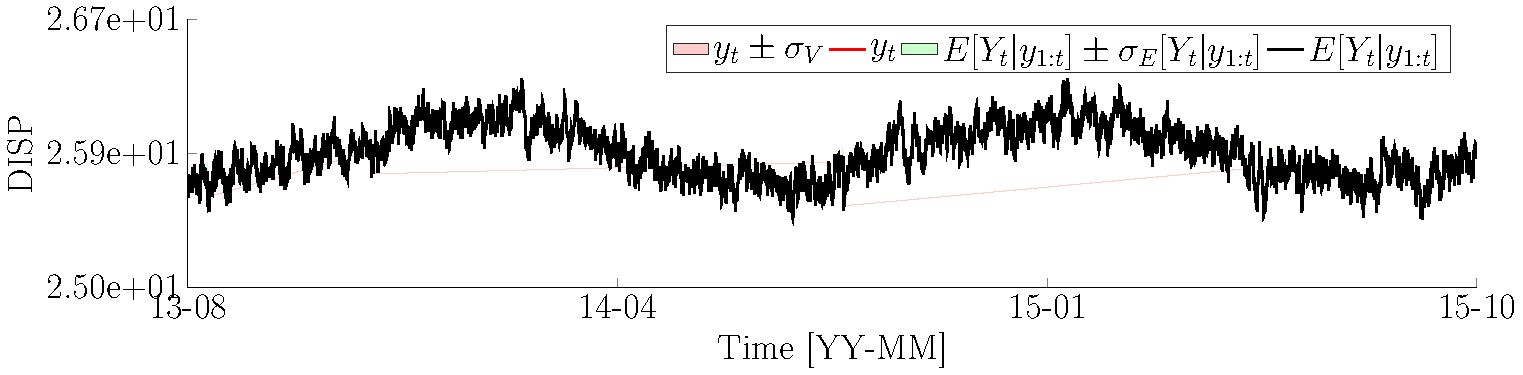
\includegraphics[width=0.9\linewidth]{./docfigs/Example_DISPSIM/optim_param_optim_initialhiddenstate/DISP_ObservedPredicted.pdf} 
\caption{Observed and estimated displacement data}
\end{subfigure}
\begin{subfigure}{\linewidth}
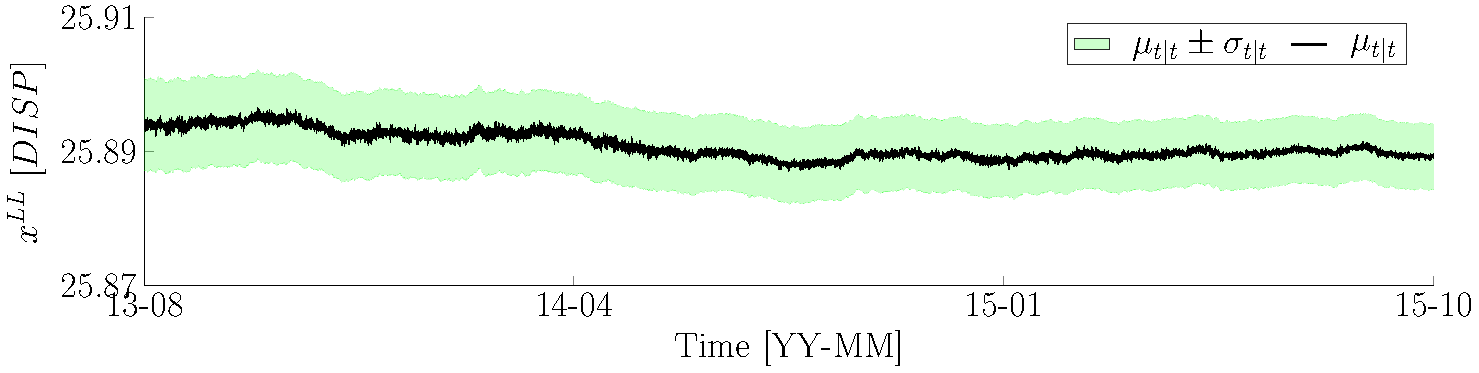
\includegraphics[width=0.9\linewidth]{./docfigs/Example_DISPSIM/optim_param_optim_initialhiddenstate/DISP_LL_1.pdf}
\caption{Estimated displacement local level component.}
\end{subfigure}
\begin{subfigure}{\linewidth}
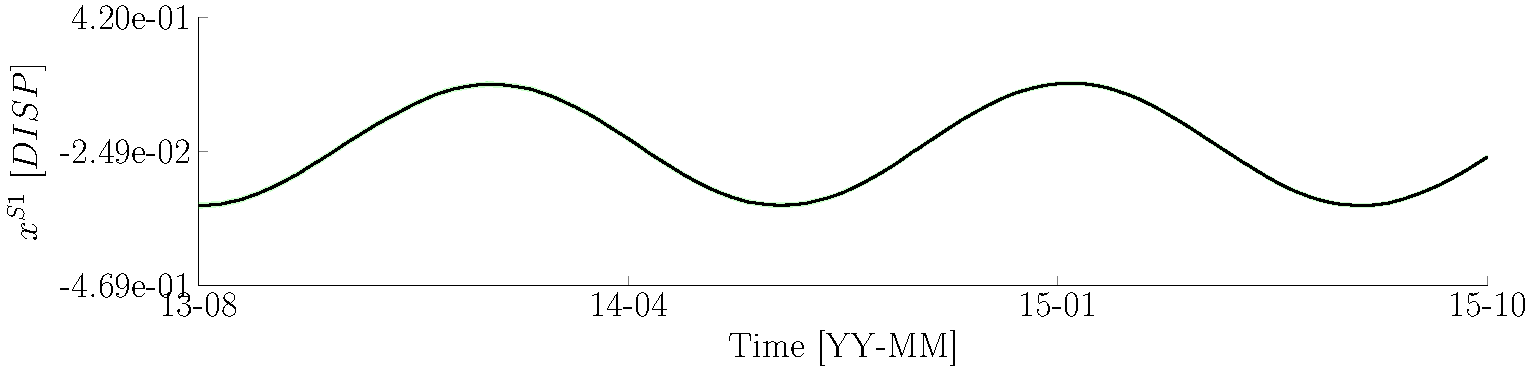
\includegraphics[width=0.9\linewidth]{./docfigs/Example_DISPSIM/optim_param_optim_initialhiddenstate/DISP_S1_2.pdf} 
\caption{Estimated displacement yearly periodic component (first hidden state)}
\end{subfigure}
\begin{subfigure}{\linewidth}
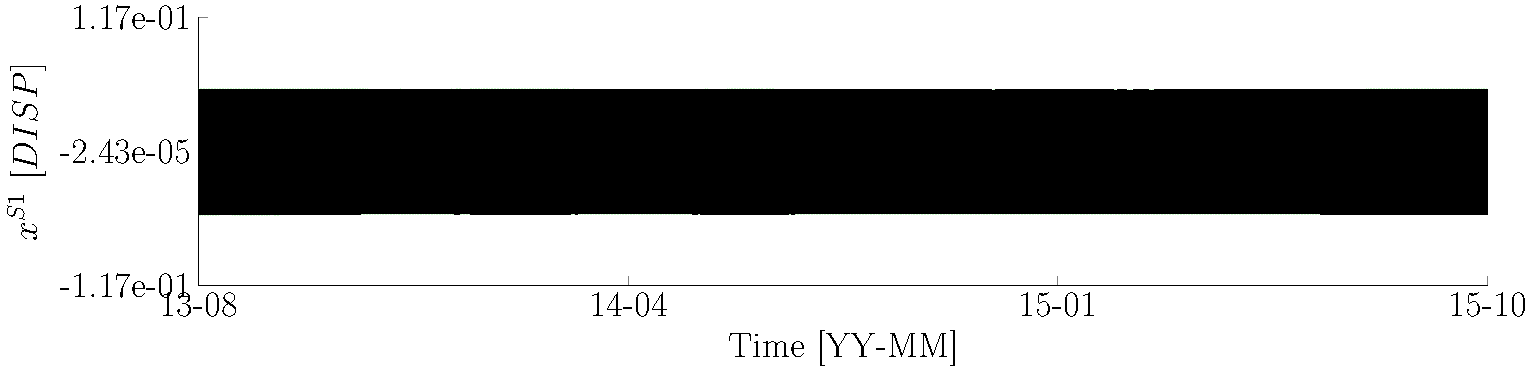
\includegraphics[width=0.9\linewidth]{./docfigs/Example_DISPSIM/optim_param_optim_initialhiddenstate/DISP_S1_4.pdf}
\caption{Estimated displacement daily periodic component (first hidden state)}
\end{subfigure}
\begin{subfigure}{\linewidth}
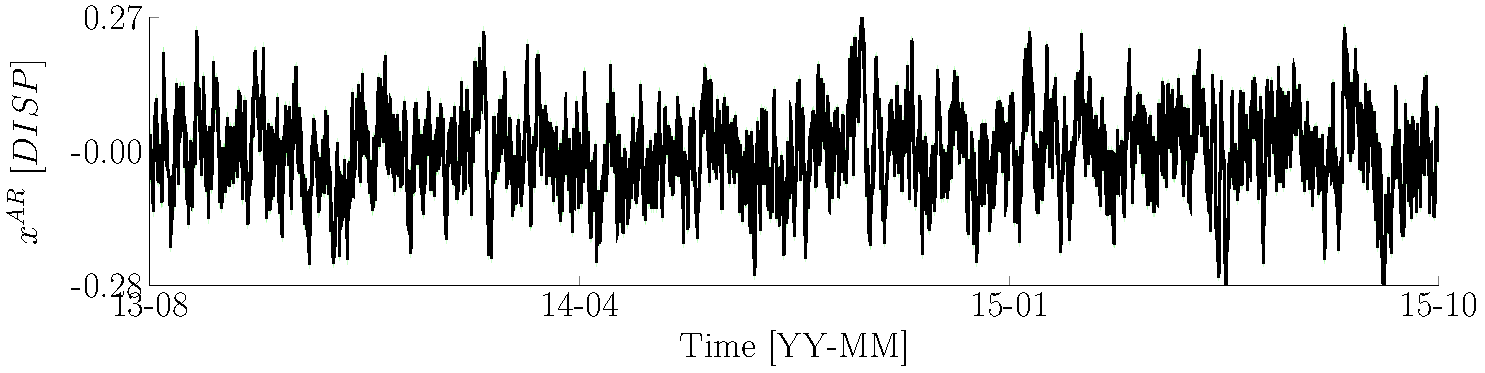
\includegraphics[width=0.9\linewidth]{./docfigs/Example_DISPSIM/optim_param_optim_initialhiddenstate/DISP_AR_6.pdf} 
\caption{Estimated displacement autoregressive component}
\end{subfigure}
\caption{Estimated results using OpenBDLM optimized model parameters and optimized initial hidden states. The hidden states are estimated from the data presented in Figure~\ref{fig:DataSummary1}a. The solid line and shaded area represent the mean and standard deviation of the estimated hidden states, respectively.}
\label{fig:Example_DISPSIMOptimizedOptimizedExample1}
\end{center}
\end{figure*}\clearpage

\section{Example \#2: dependence model between two time-series}
\label{S:ExampleDispTemp}

\subsection{Data description}

This example uses two synthetic time series data that mimics displacement and temperature data measured on a bridge.
The  Figure~\ref{fig:DataSummaryRaw2}a shows that data points exist between August 2013 and October 2015.
The timestep is non-uniform; it varies from 1 hour to 25 hours (see Figure~\ref{fig:DataSummaryRaw2}b). 
The timestep vector is not identical on each time series. 
It means that the time-series are not synchronized between each other.
The most frequent (i.e referent) time step is 1 hour for both time-series (Section~\ref{SS:NonUniform}).
There is no missing data (NaN) on the displacement time-series, but there are missing data on the temperature time series as indicated by the red crosses on the Figure~\ref{fig:DataSummaryRaw2}c.
Each red cross indicates the presence of a Not a Number (NaN) value in the time series data.
After data synchronization, the time step vectors are identical on each time series (Figure~\ref{fig:DataSummaryDefaultPreProcessed2}).
Both time-series are stationary, and they exhibit a level, a yearly and daily periodic pattern as well as an autoregressive pattern.
The periodic patterns observed on the displacement time-series is due to the temperature variations observed in the temperature time series.

\begin{figure*}[h!]
\centering
\begin{subfigure}{\linewidth}
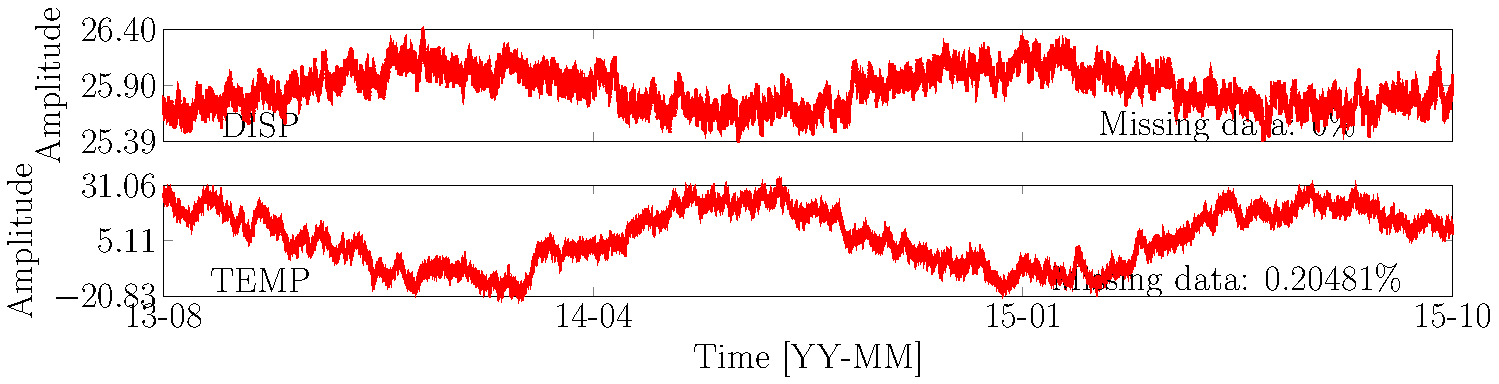
\includegraphics[width=0.9\linewidth]{./docfigs/Example_DISPTEMPSIM/raw/ALL_AMPLITUDES.pdf} 
\caption{Amplitude}
\end{subfigure}
\begin{subfigure}{\linewidth}
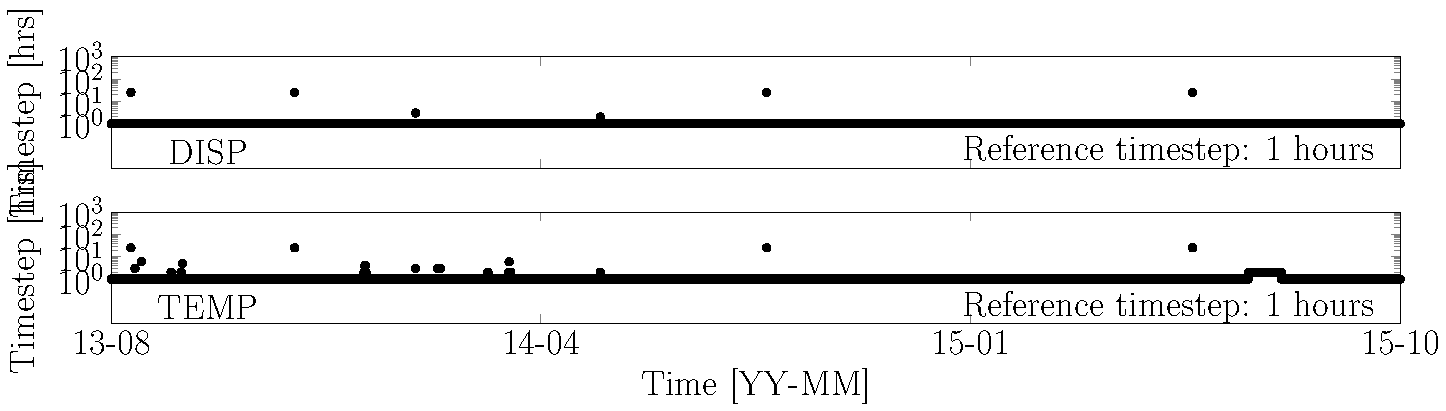
\includegraphics[width=0.9\linewidth]{./docfigs/Example_DISPTEMPSIM/raw/ALL_TIMESTEPS.pdf}
\caption{Timestep}
\end{subfigure}
\begin{subfigure}{\linewidth}
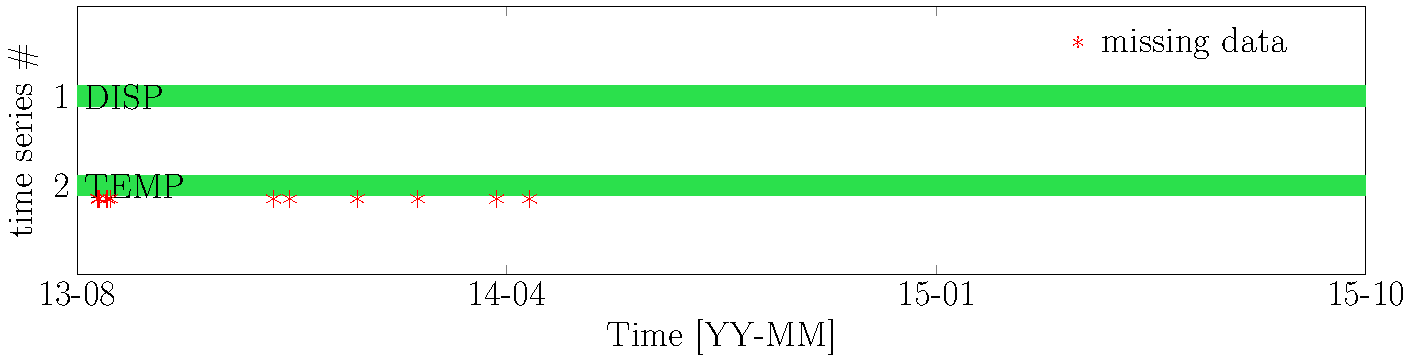
\includegraphics[width=0.9\linewidth]{./docfigs/Example_DISPTEMPSIM/raw/AVAILABILITY.pdf}
\caption{Availability}
\end{subfigure}
\caption{Data used in example \#2.}
\label{fig:DataSummaryRaw2}
\end{figure*}


\begin{figure*}[h!]
\centering
\begin{subfigure}{\linewidth}
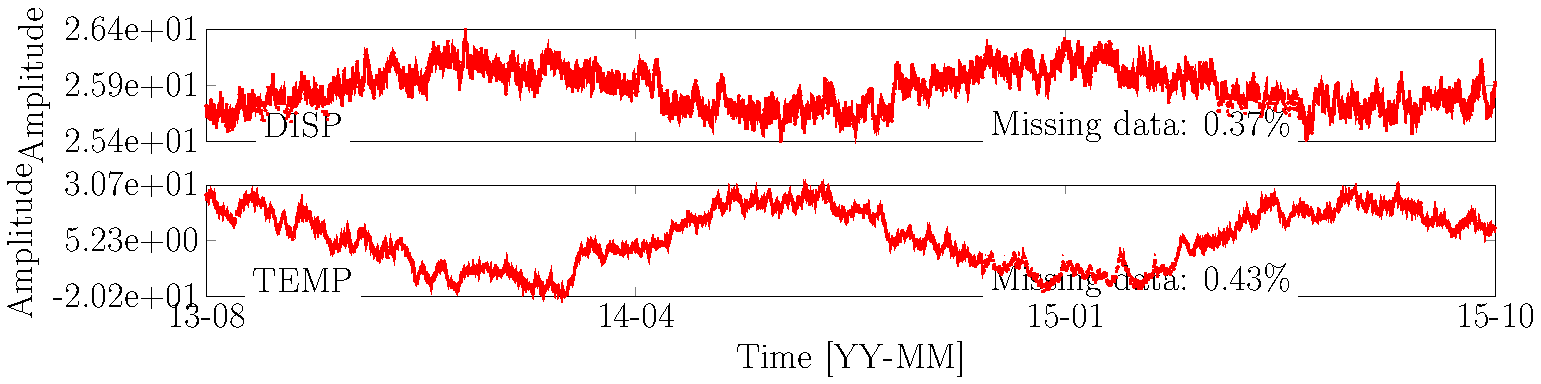
\includegraphics[width=0.9\linewidth]{./docfigs/Example_DISPTEMPSIM/preprocessed_default/ALL_AMPLITUDES.pdf} 
\caption{Amplitude}
\end{subfigure}
\begin{subfigure}{\linewidth}
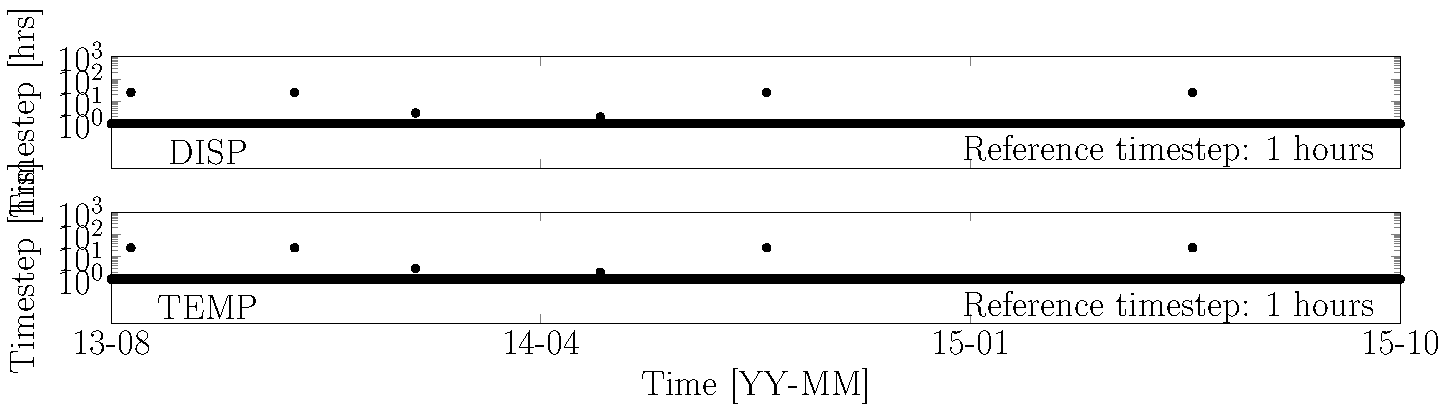
\includegraphics[width=0.9\linewidth]{./docfigs/Example_DISPTEMPSIM/preprocessed_default/ALL_TIMESTEPS.pdf}
\caption{Timestep}
\end{subfigure}
\begin{subfigure}{\linewidth}
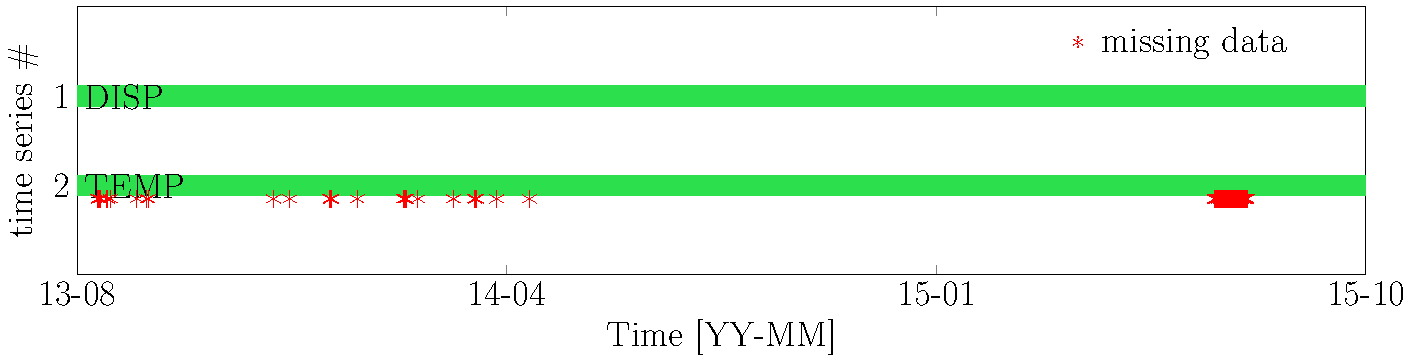
\includegraphics[width=0.9\linewidth]{./docfigs/Example_DISPTEMPSIM/preprocessed_default/AVAILABILITY.pdf}
\caption{Availability}
\end{subfigure}
\caption{Data used in example \#2 after pre-processing.}
\label{fig:DataSummaryDefaultPreProcessed2}
\end{figure*}



\subsection{Model description}
\label{SS:ModelConstructionExample2}

The model includes one model class, and the block components are 
\begin{gather*}
\textbf{x}=[x^{\mathtt{LL}}_{\text{D}}, x^{\mathtt{AR}}_{\text{D}}, x^{\mathtt{LL}}_{\text{T}}, x^{\mathtt{P1}\text{,yearly}}_{\text{T}}, x^{\mathtt{P2}\text{,yearly}}_{\text{T}}, x^{\mathtt{P1}\text{,daily}}_{\text{T}} , x^{\mathtt{P2}\text{,daily}}_{T}, x^{\mathtt{AR}}_{\text{T}}].
\end{gather*}
where $\text{D}$ and $\text{T}$ stand for displacement and temperature time-series, respectively.
The periodic patterns observed on the displacement are considered through a dependency of the displacement on the periodic block components of the temperature time-series (Section~\ref{S:Dependencies}).
The associated model parameters are
\begin{align*}
\bm\theta & =[\sigma_{w, \text{D}}^{\mathtt{LL}}, \phi^{\mathtt{AR}}_{D}, \sigma_{w, \text{D}}^{\mathtt{AR}}, \sigma_{v, \text{D}},  \\
&  \sigma_{w, \text{T}}^{\mathtt{LL}},  p^{\mathtt{P}, \text{yearly}}_{\text{T}}, \sigma_{w, \text{T}}^{\mathtt{P}, \text{yearly}} , p^{\mathtt{P}, \text{daily}}_{\text{T}} , \sigma_{w, \text{T}}^{\mathtt{P}, \text{daily}}, \phi^{\mathtt{AR}}_{\text{T}}, \sigma_{w, \text{T}}^{\mathtt{AR}}, \sigma_{v, \text{T}}].
\end{align*}
The optimized model parameters values computed using the Newton-Raphson algorithm (see~\ref{SS:THModelParameterEstimation}) are
\begin{align*}
 \bm\theta^{\text{*}}& =[0, 0.97, 0.019, 7.42\times10^{-7},  \\
 & 0, 365.2422, 0, 1, 0, 0.99, 0.43, 2.67\times10^{-5}, -0.011, 0.0711, 0.000292 ]
\end{align*}
The optimized initial hidden states mean and covariance values are 
\begin{align*}
\bm \mu^{*}_{0} & = [	 25.9  ,	-0.0595	, 5.45  	, 17.6  ,	-0.934	, 0.678 ,	0.41  ,	2.1]^{\intercal}, \text{and} \\
\bm\Sigma^{*}_{0} & = \text{diag} [	3.71\times10^{-5},	0.000457	, 0.287 	, 0.263 ,	0.265 	,8.14\times10^{-5}	, \\
 & 8.14\times10^{-5}	, 0.71    ], 
 \end{align*}
 respectively.
The hidden states computed using the estimated model parameters and initial hidden states are presented in Figure~\ref{fig:DISPTEMPSIMOptimizedOptimizedExample2}.


\subsection{Run the example from pre-existing configuration file}
There is a configuration file CFG\_Example\_DISPTEMP\_optim.m which is located in the ``config\_files'' folder of the OpenBDLM package.
CFG\_Example\_DISPTEMP\_optim.m contains the optimized model parameters and optimized initial hidden states values.
There is also a data file DATA\_Example\_DISPTEMP\_optim.mat that is located in the ``data/mat'' subfolder.
Therefore, it is possible to run the example \#1 by following the following steps from the \MATLAB{} command line:
\begin{enumerate}
\item Start OpenBDLM. Type \colorbox{light-gray}{\lstinline[basicstyle = \mlttfamily \small, backgroundcolor = \color{light-gray}]!OpenBDLM_main('CFG_Example_DISPTEMP_optim.m');!}.
\item Access hidden states estimation menu. Type \colorbox{light-gray}{\lstinline[basicstyle = \mlttfamily \small, backgroundcolor = \color{light-gray}]!3!}.
\item Run the Kalman filter to estimate the hidden states. Type \colorbox{light-gray}{\lstinline[basicstyle = \mlttfamily \small, backgroundcolor = \color{light-gray}]!1!}.
\item Save and quit. Type \colorbox{light-gray}{\lstinline[basicstyle = \mlttfamily \small, backgroundcolor = \color{light-gray}]!Q!}.
\end{enumerate}


\subsection{Run the example from command line interaction}

The analysis of a new dataset usually requires to start from scratch.
This section explains how to run the example \#1 from scratch, that is, how to load the data presented in Figure~\ref{fig:DataSummaryRaw2}, configure the model, estimate the model parameters and estimate the hidden states.
This may be done by following the following steps from the \MATLAB{} command line:
\begin{enumerate}
\item Start OpenBDLM. Type \colorbox{light-gray}{\lstinline[basicstyle = \mlttfamily \small, backgroundcolor = \color{light-gray}]!OpenBDLM_main();!}.
\item Choose the interactive tool. Type \colorbox{light-gray}{\lstinline[basicstyle = \mlttfamily \small, backgroundcolor = \color{light-gray}]!0!}.
\item Enter the project name. Type \colorbox{light-gray}{\lstinline[basicstyle = \mlttfamily \small, backgroundcolor = \color{light-gray}]!Example_DISPTEMP!}. 
\item Disregard generating synthetic data. Type \colorbox{light-gray}{\lstinline[basicstyle = \mlttfamily \small, backgroundcolor = \color{light-gray}]!no!}. 
\item Load new data. Type \colorbox{light-gray}{\lstinline[basicstyle = \mlttfamily \small, backgroundcolor = \color{light-gray}]!0!}.
\item Select the /data/csv/Example\_DISPTEMP[/Example\_DISPTEMP\_DISP.csv and /data/csv/Example\_DISP/Example\_DISPTEMP\_TEMP.csv data files from the graphical user interface. 
\item Save and continue without pre-processing. Type \colorbox{light-gray}{\lstinline[basicstyle = \mlttfamily \small, backgroundcolor = \color{light-gray}]!7!}. 
\item Select the number of model classes. Type \colorbox{light-gray}{\lstinline[basicstyle = \mlttfamily \small, backgroundcolor = \color{light-gray}]!1!}. 
\item Select dependency for the time series \#1. Type \colorbox{light-gray}{\lstinline[basicstyle = \mlttfamily \small, backgroundcolor = \color{light-gray}]![2]!}.
\item Select dependency for the time series \#2. Type \colorbox{light-gray}{\lstinline[basicstyle = \mlttfamily \small, backgroundcolor = \color{light-gray}]![0]!}.
\item Select the model block components for time series \#1. Type \colorbox{light-gray}{\lstinline[basicstyle = \mlttfamily \small, backgroundcolor = \color{light-gray}]![11 41]!}.
\item Select the model block components for time series \#2. Type \colorbox{light-gray}{\lstinline[basicstyle = \mlttfamily \small, backgroundcolor = \color{light-gray}]![11 31 31 41]!}.
\item Access model parameter estimation menu. Type \colorbox{light-gray}{\lstinline[basicstyle = \mlttfamily \small, backgroundcolor = \color{light-gray}]!1!}. 
\item Start Newton-Raphson algorithm. Type \colorbox{light-gray}{\lstinline[basicstyle = \mlttfamily \small, backgroundcolor = \color{light-gray}]!1!}. Once the algorithm is converged, the optimized model parameters values should be close to the values presented in Section~\ref{SS:ModelConstructionExample2}. See also \footnote{Note that it is possible to get slightly different value of parameters with the same performance.}.
\item Estimate the initial hidden states values. Type \colorbox{light-gray}{\lstinline[basicstyle = \mlttfamily \small, backgroundcolor = \color{light-gray}]!2!}.
\item Access hidden states estimation menu. Type \colorbox{light-gray}{\lstinline[basicstyle = \mlttfamily \small, backgroundcolor = \color{light-gray}]!3!}. 
\item Estimate the hidden states using Kalman filter. Type \colorbox{light-gray}{\lstinline[basicstyle = \mlttfamily \small, backgroundcolor = \color{light-gray}]!1!}. The estimation should be similar to the results presented in Figure~\ref{fig:Example_DISPTEMPSIMOptimizedOptimizedExample2}.
\item Access export menu. Type \colorbox{light-gray}{\lstinline[basicstyle = \mlttfamily \small, backgroundcolor = \color{light-gray}]!17!}. 
\item Export the current project in a configuration file. Type \colorbox{light-gray}{\lstinline[basicstyle = \mlttfamily \small, backgroundcolor = \color{light-gray}]!1!}.
\item Save and quit OpenBDLM. Type \colorbox{light-gray}{\lstinline[basicstyle = \mlttfamily \small, backgroundcolor = \color{light-gray}]!Q!}.
\end{enumerate}




%\subsection{Step 4: configure the model}
%
%The next step is to configure the model.
%First, the program requests the number of model class.
%In this exemple, the time series data looks stationary and we are not interested in anomaly detection, and therefore we type \colorbox{light-gray}{\lstinline[basicstyle = \mlttfamily \small, backgroundcolor = \color{light-gray}]!1!}.
%Secondly, because there are several time series, OpenBDLM needs to know if there are dependencies between the time-series.
%Typing \colorbox{light-gray}{\lstinline[basicstyle = \mlttfamily \small, backgroundcolor = \color{light-gray}]!2!} for the first time-series, and \colorbox{light-gray}{\lstinline[basicstyle = \mlttfamily \small, backgroundcolor = \color{light-gray}]!0!} for the second time series means that the model will consider the irreversible components (if any) of the second (temperature) time-series as covariates to describe the irreversible patterns observed in the first (displacement) time-series.
%Then, OpenBDLM asks for the type of block component for each time-series. 
%Type \colorbox{light-gray}{\lstinline[basicstyle = \mlttfamily \small, backgroundcolor = \color{light-gray}]![11 41]!} for the displacement time series and \colorbox{light-gray}{\lstinline[basicstyle = \mlttfamily \small, backgroundcolor = \color{light-gray}]![11 31 31 41]!} for the temperature time series.
%The yearly and daily periodic patterns observed in the displacement time-series are modelled using the dependence on the periodic components defined for modelling the temperature time series data.
%Note that because an autoregressive component is chosen for the displacement time series data, the time-dependent model error on the displacement is modelled using a dependence on the autoregressive component of the temperature time series data, as well as an independent autoregressive component.
%The  output on \MATLAB{} command window during interactive model configuration is presented in Listing~\ref{LST:OpenBDLMModelConfigureExample2}.
%Type $\dlsh$ to valid.
%The model is then built, a \lstinline[basicstyle = \mlttfamily \small, backgroundcolor = \color{light-gray}]!DATA_DISPTEMP.mat! binary data file, a \lstinline[basicstyle = \mlttfamily \small, backgroundcolor = \color{light-gray}]!CFG_DISPTEMP.m! configuration file, as well as a \lstinline[basicstyle = \mlttfamily \small, backgroundcolor = \color{light-gray}]!PROJ_DISPTEMP.mat! project file are created.
%The OpenBLDM main menu must appear on the \MATLAB{} command window (see Listing~\ref{LST:OpenBDLMMainMenu}).
%Type \colorbox{light-gray}{\lstinline[basicstyle = \mlttfamily \small, backgroundcolor = \color{light-gray}]!Q!} to save and quit.



% \begin{lstlisting}[ frame = single, basicstyle = \mlttfamily \small, caption = { \MATLAB{} command window output during model configuration}, label = LST:OpenBDLMModelConfigureExample2,  float =h!, linewidth=\linewidth, captionpos=b, breaklines=true]
%- Identifies dependence between time series; use [0] to indicate no dependence
%    time serie #1 depends on time series # >> [2]
%
%- Identifies dependence between time series; use [0] to indicate no dependence
%    time serie #2 depends on time series # >> [0]
%
%- How many model classes do you want for each time-series? 
%     choice >> 1
%     
%     ------------------------------------
%          BDLM Component reference numbers
%     ------------------------------------
%     11: Local level 
%     12: Local trend 
%     13: Local acceleration 
%     21: Local level compatible with local trend 
%     22: Local level compatible with local acceleration 
%     23: Local trend compatible with local acceleration 
%     31: Periodic 
%     41: Autoregressive process (AR(1)) 
%     51: Kernel regression 
%     61: Level Intervention 
%     --------------------------------------
%
%- Identify components for time series #1; e.g. [11 31 41]
%     choice >> [11 41]
%
%- Identify components for time series #2; e.g. [11 31 41]
%     choice >> [11 31 31 41]
%
%     Building model...
%     Saving project...
%     Project saved in saved_projects/PROJ_Example_DISPTEMP.mat. 
%     Printing configuration file...
%     Saving data...
%     Database saved in data/mat/DATA_Example_DISPTEMP.mat 
%     Configuration file saved in config_files/CFG_Example_DISPTEMP.m. 
%\end{lstlisting}


%\subsection{Step 5: open the configuration file}
%
%After the data loading and the model configuration, a configuration file named \lstinline[basicstyle = \mlttfamily \small, backgroundcolor = \color{light-gray}]!CFG_Example_DISPTEMP.m! configuration file is automatically created and saved in ``config\_files'' folder.
%Open the configuration file from \MATLAB{} command line by typing  \colorbox{light-gray}{\lstinline[basicstyle = \mlttfamily \small, backgroundcolor = \color{light-gray}]!edit CFG_Example_DISPTEMP.m!}.
%%The first part of this configuration file as it should appear on the \MATLAB{} editor is shown in Listing~\ref{LST:CFGFileExample1}.
%The Model parameters section of the configuration file shows that the model totalizes 15 model parameters, that is 
%\begin{gather*}
%\bm\theta=\{\sigma_{w, \text{D}}^{LL},  \phi^{AR}_{\text{D}}, \sigma_{w,\text{D}}^{AR} ,\sigma_{v,\text{D}},  \\
% \sigma_{w, \text{T}}^{LL}, p^{\text{PD1}}_{\text{T}}, \sigma_{w,\text{T}}^{\text{PD1}} , p^{\text{PD2}}_{T}, \sigma_{w, \text{T}}^{\text{PD2}}, \phi^{AR}_{T}, \sigma_{w, \text{T}}^{AR}, \sigma_{v,\text{T}}, \phi^{\text{D}|\text{T}}_{PD1}, \phi^{\text{D}|\text{T}}_{PD2},  \phi^{\text{D}|\text{T}}_{AR}\}.
%\end{gather*}
%%The default value of the model parameters are assigned  using heuristic knowledge or computed from the data using statistics on the data.
%The default model parameters values are 
%\begin{gather*}
%\bm\theta^{\text{default}}=\{0, 0.75, 0.017, 0.0087, \\
%0, 365.24, 0, 1, 0, 0.75, 1.2905, 0.64526, 0.5, 0.5, 0.5 \}.
%\end{gather*}
%%In the same manner, default value for the initial hidden states are assigned using heuristic knowledge or computed using statistics on the data.
%The default initial hidden states mean  and covariance values are 
%\begin{align*}
% \bm \mu^{\text{default}}_{0} & = [	25.7  ,	0  ,   	16.7  	, 5     ,	0   ,  	5   ,  	0    , 	0        ]^{\intercal}, \text{and} \\
% \text{diag}(\bm\Sigma^{\text{default}}_{0})  & = [	0.122, 	0.0305,	666,   	666,   	666,   	666,   	666 ,  	167     ],
%\end{align*}
%respectively.
%%$\bm \mu^{\text{default}}_{0} = [	25.7  ,	0  ,   	16.7  	, 5     ,	0   ,  	5   ,  	0    , 	0        ]$, and $\text{diag}(\bm\Sigma^{\text{default}}_{0}) = [	0.122, 	0.0305,	666,   	666,   	666,   	666,   	666 ,  	167     ]$, respectively.
%In the Options section, change \lstinline[basicstyle = \mlttfamily \small, backgroundcolor = \color{light-gray}]!misc.options.MethodStateEstimation='kalman'! to \lstinline[basicstyle = \mlttfamily \small, backgroundcolor = \color{light-gray}]!misc.options.MethodStateEstimation='UD'!. 
%In this specific example, the presence of missing data requires the use of UD computations instead of the standard, default, Kalman computation.
%Note that the choice about UD or Kalman is problem dependent. 
%
%\subsection{Step 6: estimate the hidden states}
%
%Type \colorbox{light-gray}{\lstinline[basicstyle = \mlttfamily \small, backgroundcolor = \color{light-gray}]!OpenBDLM_main('CFG_Example_DISPTEMP.m');!} in the \MATLAB{} command line.
%Once, the main menu appears, type  \colorbox{light-gray}{\lstinline[basicstyle = \mlttfamily \small, backgroundcolor = \color{light-gray}]!3!}, then \colorbox{light-gray}{\lstinline[basicstyle = \mlttfamily \small, backgroundcolor = \color{light-gray}]!1!} to estimate the filtered hidden states using the default model parameters and default initial hidden states values.
%The value of the log-likelihood is $-3800091$.
%The estimated hidden states are presented in Figure~\ref{fig:DISPTEMPSIMDefaultDefaultExample2}.


%\subsection{Step 7: estimate the model parameters from the data}
%
%Type \colorbox{light-gray}{\lstinline[basicstyle = \mlttfamily \small, backgroundcolor = \color{light-gray}]!OpenBDLM_main('CFG_Example_DISPTEMP.m');!} in the \MATLAB{} command line.
%Once, the main menu appears, type  \colorbox{light-gray}{\lstinline[basicstyle = \mlttfamily \small, backgroundcolor = \color{light-gray}]!1!}, then \colorbox{light-gray}{\lstinline[basicstyle = \mlttfamily \small, backgroundcolor = \color{light-gray}]!1!} to estimate the model parameters using Newton-Raphson (type  \colorbox{light-gray}{\lstinline[basicstyle = \mlttfamily \small, backgroundcolor = \color{light-gray}]!1!} to use the Stochastic Gradient instead).
%The model parameters learning procedure should start (see for example Listing~\ref{LST:OpenBLDMModelParameterLearning}).
%Note that, by default, OpenBDLM considers that the parameters $\sigma_{w, \text{D}}^{LL}$, $\sigma_{w, \text{T}}^{LL}$, $p^{\text{PD1}}_{\text{T}}$, $\sigma_{w, \text{T}}^{\text{PD1}}$ , $p^{\text{PD2}}_{\text{T}}$, $\sigma_{w,\text{T}}^{\text{PD2}}$ are known.
%Therefore, there are nine model parameters to be learned from the data in this example.
%The estimation of the model parameters may take several hours.
%Therefore, press combinations \colorbox{light-gray}{\lstinline[basicstyle = \mlttfamily \small, backgroundcolor = \color{light-gray}]!Ctrl!} + \colorbox{light-gray}{\lstinline[basicstyle = \mlttfamily \small, backgroundcolor = \color{light-gray}]!c!} to abort the process.
%Once the algorithm is converged, the optimized model parameters values should be close to  \footnote{Note that it is possible to get slightly different value of parameters with the same performance.}
%\begin{gather*}
% \bm\theta^{\text{*}}=\{0, 0.97, 0.019, 7.42\times10^{-7}, 0, 365.2422, 0, 1, 0, 0.99, 0.43, 2.67\times10^{-5},  \\
% -0.011, 0.0711, 0.000292 \}
%\end{gather*}


%\subsection{Step 8: estimate the hidden states using the optimized model parameters. values}
%
%In the ``examples/Example\_DISPTEMP'' folder, there is a configuration file named \lstinline[basicstyle = \mlttfamily \small, backgroundcolor = \color{light-gray}]!CFG_Example_DISPTEMP_optim.m! that contains optimized model parameters estimated using the Newton-Raphson algorithm.
%Copy and paste \lstinline[basicstyle = \mlttfamily \small, backgroundcolor = \color{light-gray}]!CFG_Example_DISPTEMP_optim.m! from  the ``examples/Example\_DISPTEMP'' subfolder  to the ``config\_files'' folder.
%Type \colorbox{light-gray}{\lstinline[basicstyle = \mlttfamily \small, backgroundcolor = \color{light-gray}]!OpenBDLM_main('CFG_Example_DISPTEMP_optim.m');!} in the \MATLAB{} command line to load the configuration file  \lstinline[basicstyle = \mlttfamily \small, backgroundcolor = \color{light-gray}]!CFG_Example_DISPTEMP_optim.m!.
%Once the main menu appears, type  \colorbox{light-gray}{\lstinline[basicstyle = \mlttfamily \small, backgroundcolor = \color{light-gray}]!3!}, then \colorbox{light-gray}{\lstinline[basicstyle = \mlttfamily \small, backgroundcolor = \color{light-gray}]!1!} to estimate the filtered hidden states using the optimized model parameters and default initial hidden states values.
%The value of the log-likelihood is now $38085$.
%The estimated hidden states are presented in Figure~\ref{fig:DISPTEMPSIMOptimizedDefaultExample2}.

%\subsection{Step 9: estimate the initial hidden states}
%
%Type \colorbox{light-gray}{\lstinline[basicstyle = \mlttfamily \small, backgroundcolor = \color{light-gray}]!OpenBDLM_main('CFG_Example_DISPTEMP_optim.m');!} in the \MATLAB{} command line.
%Then, type  \colorbox{light-gray}{\lstinline[basicstyle = \mlttfamily \small, backgroundcolor = \color{light-gray}]!2!}, to optimize the initial hidden states value.
%The estimated initial hidden states mean and covariance values are 
%\begin{align*}
%\bm \mu^{*}_{0} & = [	 25.9  ,	-0.0595	, 5.45  	, 17.6  ,	-0.934	, 0.678 ,	0.41  ,	2.1]^{\intercal}, \text{and} \\
% \text{diag}(\bm\Sigma^{*}_{0}) & = [	3.71\times10^{-5},	0.000457	, 0.287 	, 0.263 ,	0.265 	,8.14\times10^{-5}	, \\
% & 8.14\times10^{-5}	, 0.71    ], 
% \end{align*}
% respectively.
%Once it is done, type  \colorbox{light-gray}{\lstinline[basicstyle = \mlttfamily \small, backgroundcolor = \color{light-gray}]!3!}, and then  \colorbox{light-gray}{\lstinline[basicstyle = \mlttfamily \small, backgroundcolor = \color{light-gray}]!1!} to compute the filtered hidden states using the optimized model parameters and optimized initial hidden states.
%The value of the log-likelihood is $38120$.
%The estimated hidden states are presented in Figure~\ref{fig:DISPTEMPSIMOptimizedOptimizedExample2}.


%\begin{figure*}[h!]
%\centering
%\begin{subfigure}{\linewidth}
%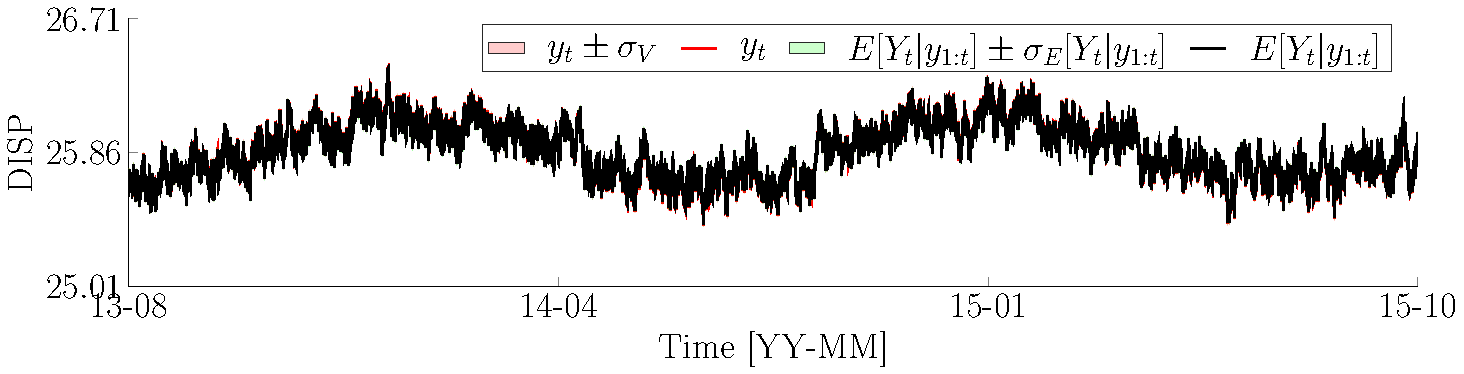
\includegraphics[width=0.9\linewidth]{./docfigs/Example_DISPTEMPSIM/default/DISP_ObservedPredicted.pdf}
%\caption{Observed and estimated displacement data} 
%\end{subfigure}
%\begin{subfigure}{\linewidth}
%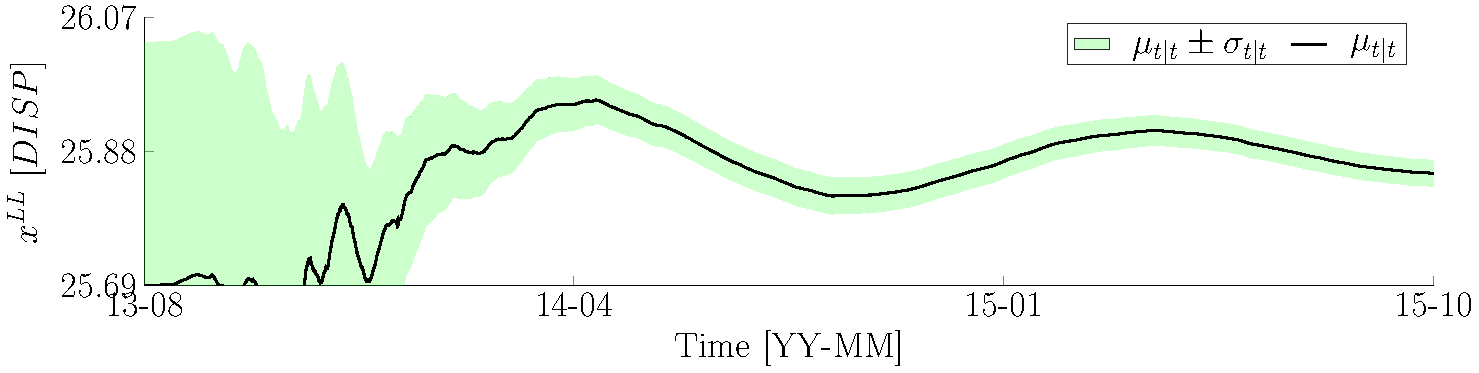
\includegraphics[width=0.9\linewidth]{./docfigs/Example_DISPTEMPSIM/default/DISP_LL_1.pdf}
%\caption{Estimated displacement local level component.}
%\end{subfigure}
%\begin{subfigure}{\linewidth}
%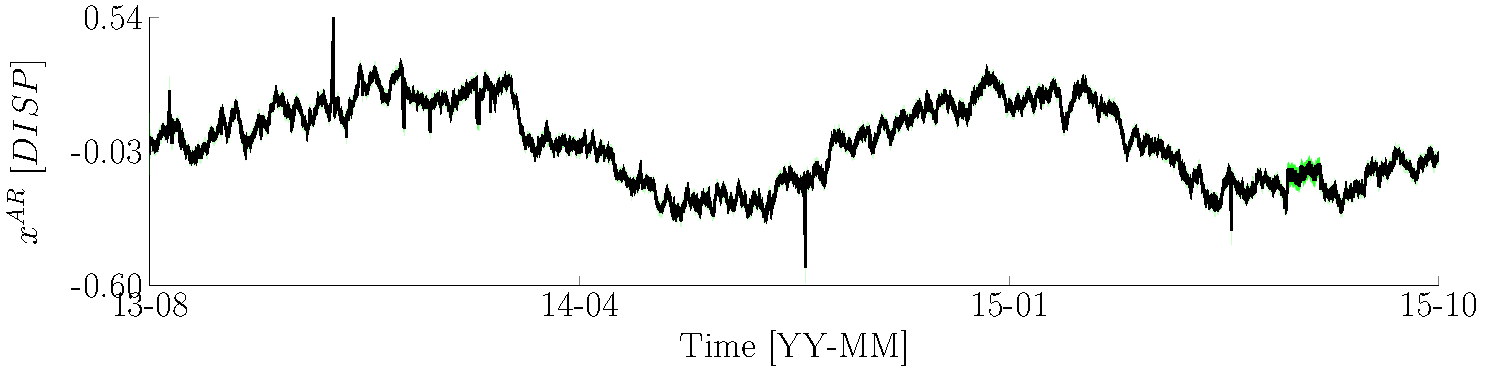
\includegraphics[width=0.9\linewidth]{./docfigs/Example_DISPTEMPSIM/default/DISP_AR_2.pdf}
%\caption{Estimated displacement autoregressive component.}
%\end{subfigure}
%\end{figure*}
%\begin{figure*}[h!]
%\ContinuedFloat
%\begin{subfigure}{\linewidth}
%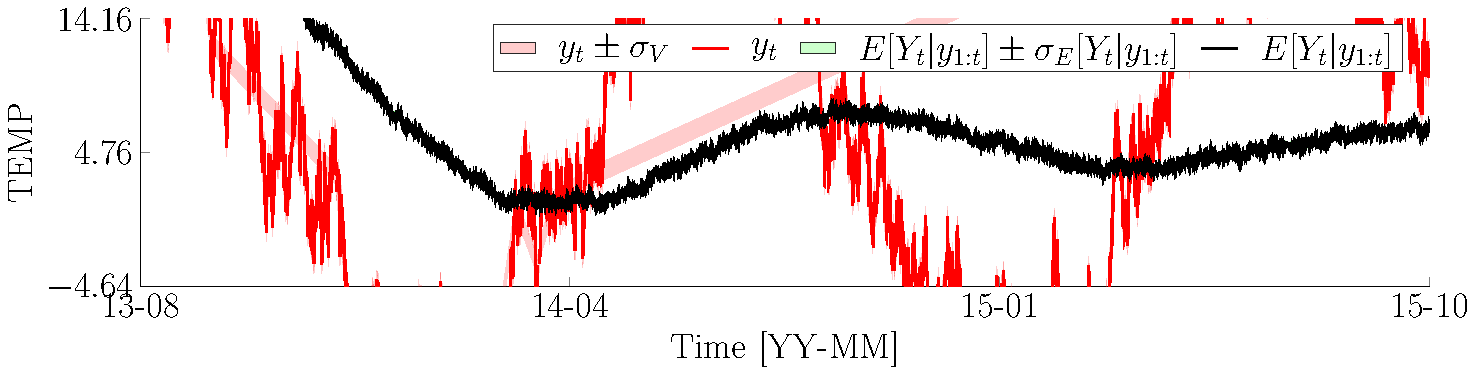
\includegraphics[width=0.9\linewidth]{./docfigs/Example_DISPTEMPSIM/default/TEMP_ObservedPredicted.pdf} 
%\caption{Observed and estimated temperature data}
%\end{subfigure}
%\begin{subfigure}{\linewidth}
%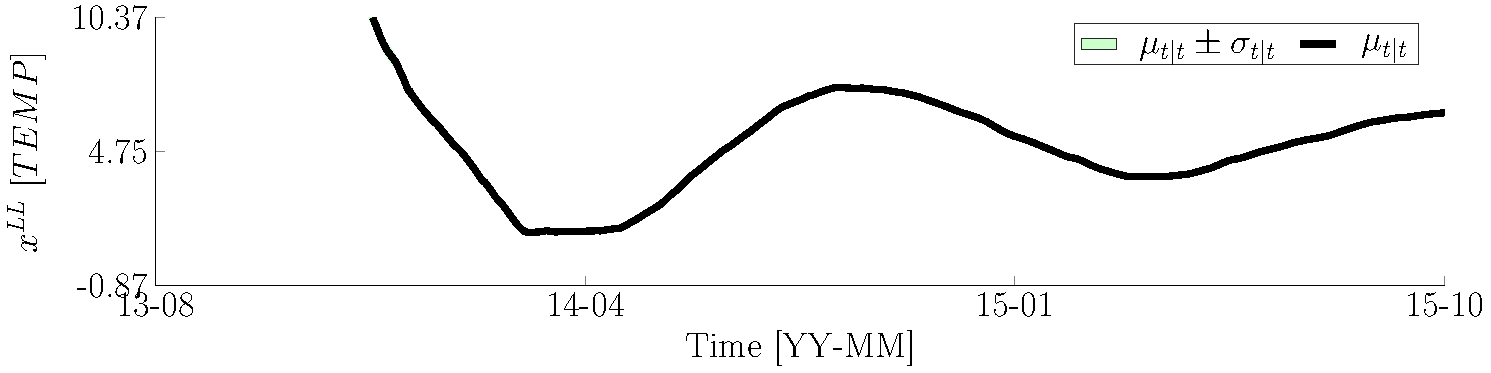
\includegraphics[width=0.9\linewidth]{./docfigs/Example_DISPTEMPSIM/default/TEMP_LL_1.pdf} 
%\caption{Estimated temperature local level component.}
%\end{subfigure}
%\begin{subfigure}{\linewidth}
%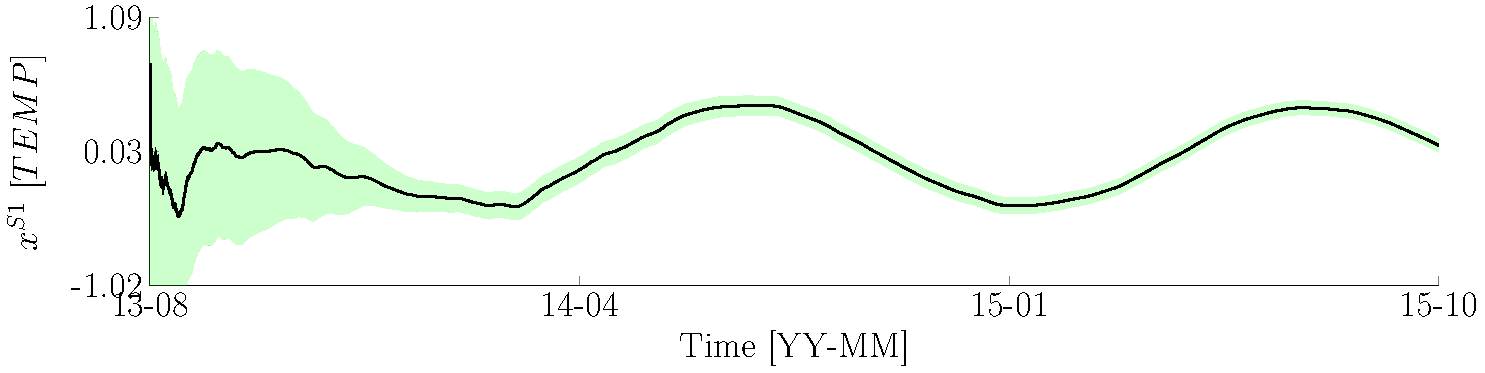
\includegraphics[width=0.9\linewidth]{./docfigs/Example_DISPTEMPSIM/default/TEMP_S1_2.pdf} 
%\caption{Estimated temperature yearly component (first hidden state)}
%\end{subfigure}
%\begin{subfigure}{\linewidth}
%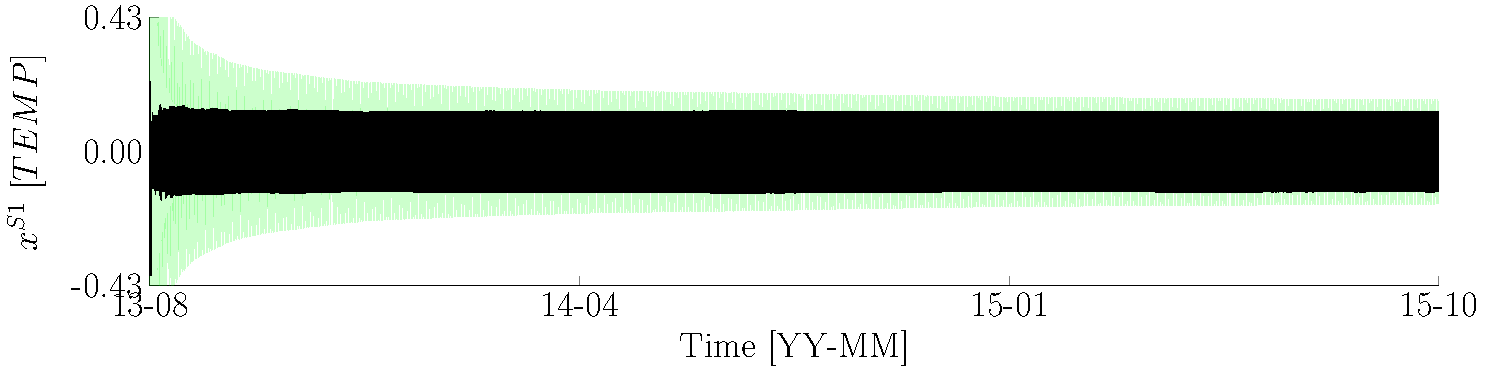
\includegraphics[width=0.9\linewidth]{./docfigs/Example_DISPTEMPSIM/default/TEMP_S1_4.pdf} 
%\caption{Estimated temperature daily component (first hidden state)}
%\end{subfigure}
%\begin{subfigure}{\linewidth}
%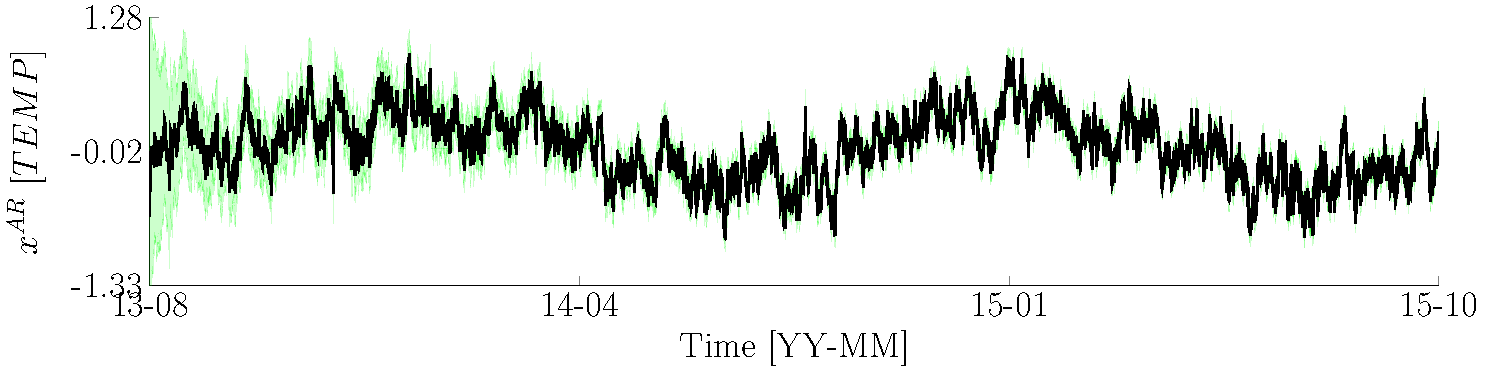
\includegraphics[width=0.9\linewidth]{./docfigs/Example_DISPTEMPSIM/default/TEMP_AR_6.pdf} 
%\caption{Estimated temperature autoregressive component}
%\end{subfigure}
%\caption{Estimated results using OpenBDLM default model parameters and default initial hidden states. The hidden states are estimated from the data presented in Figure~\ref{fig:DataSummaryDefaultPreProcessed2}a. The solid line and shaded area represent the mean and standard deviation of the estimated hidden states, respectively.}
%\label{fig:DISPTEMPSIMDefaultDefaultExample2}
%\end{figure*}

%\begin{figure*}[h!]
%\centering
%\begin{subfigure}{\linewidth}
%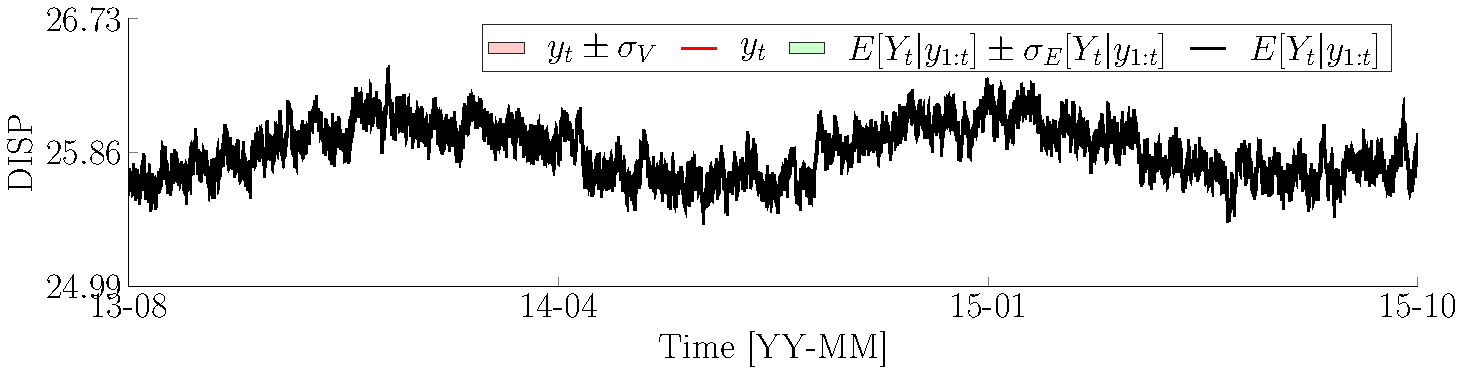
\includegraphics[width=0.9\linewidth]{./docfigs/Example_DISPTEMPSIM/optim_param_default_initialhiddenstate/DISP_ObservedPredicted.pdf}
%\caption{Observed and estimated displacement data} 
%\end{subfigure}
%\begin{subfigure}{\linewidth}
%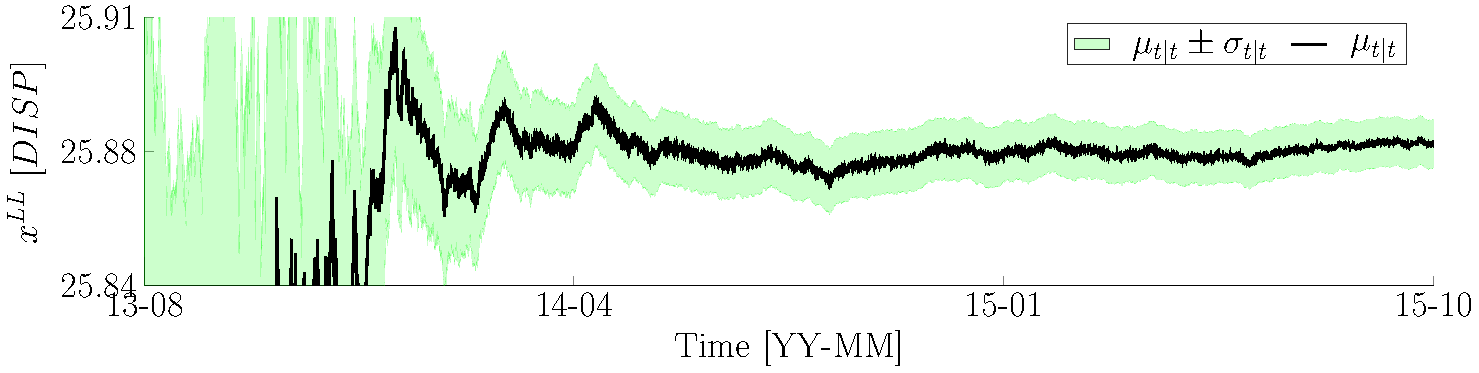
\includegraphics[width=0.9\linewidth]{./docfigs/Example_DISPTEMPSIM/optim_param_default_initialhiddenstate/DISP_LL_1.pdf}
%\caption{Estimated displacement local level component.}
%\end{subfigure}
%\begin{subfigure}{\linewidth}
%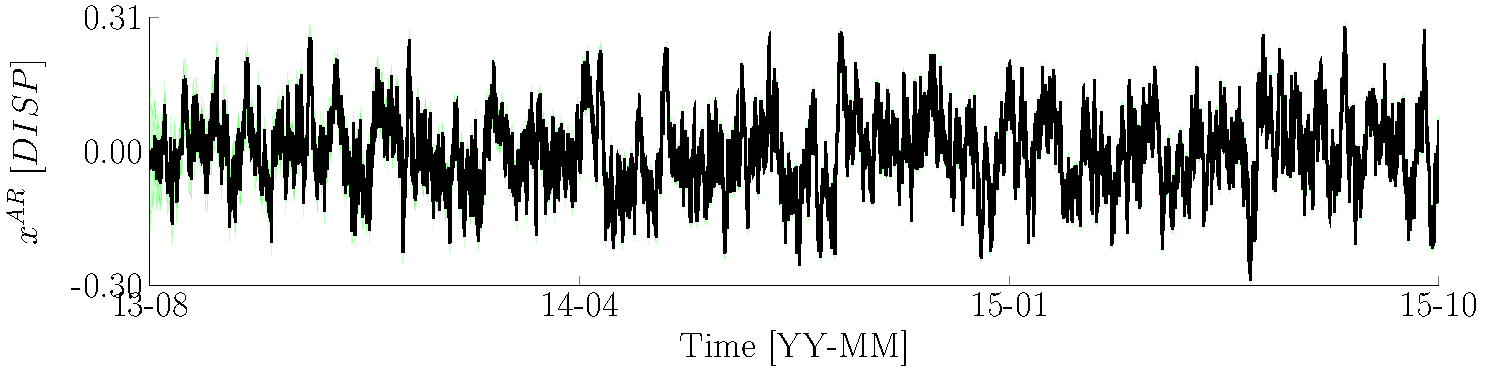
\includegraphics[width=0.9\linewidth]{./docfigs/Example_DISPTEMPSIM/optim_param_default_initialhiddenstate/DISP_AR_2.pdf}
%\caption{Estimated displacement autoregressive component.}
%\end{subfigure}
%\end{figure*}
%\begin{figure*}[h!]
%\ContinuedFloat
%\begin{subfigure}{\linewidth}
%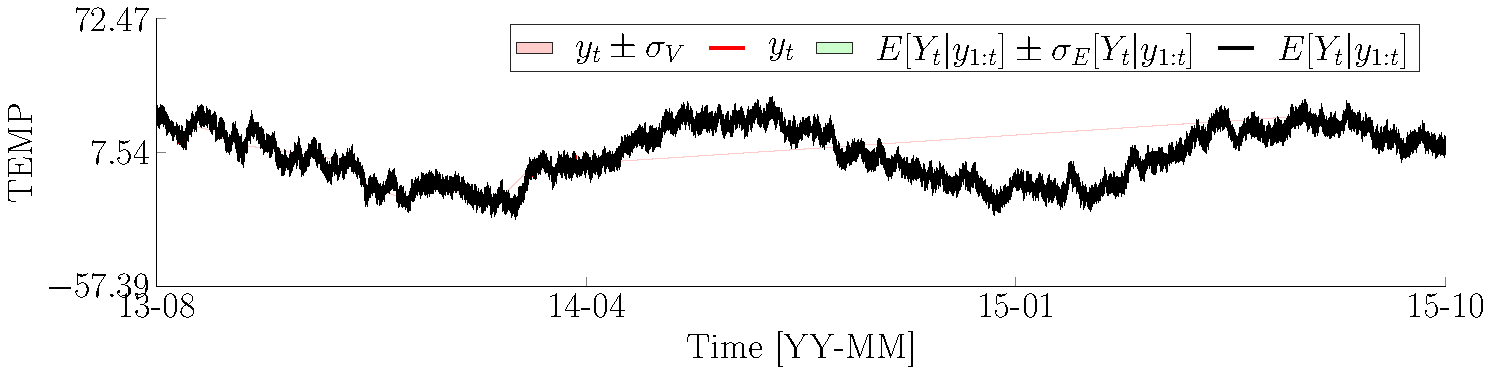
\includegraphics[width=0.9\linewidth]{./docfigs/Example_DISPTEMPSIM/optim_param_default_initialhiddenstate/TEMP_ObservedPredicted.pdf} 
%\caption{Observed and estimated temperature data}
%\end{subfigure}
%\begin{subfigure}{\linewidth}
%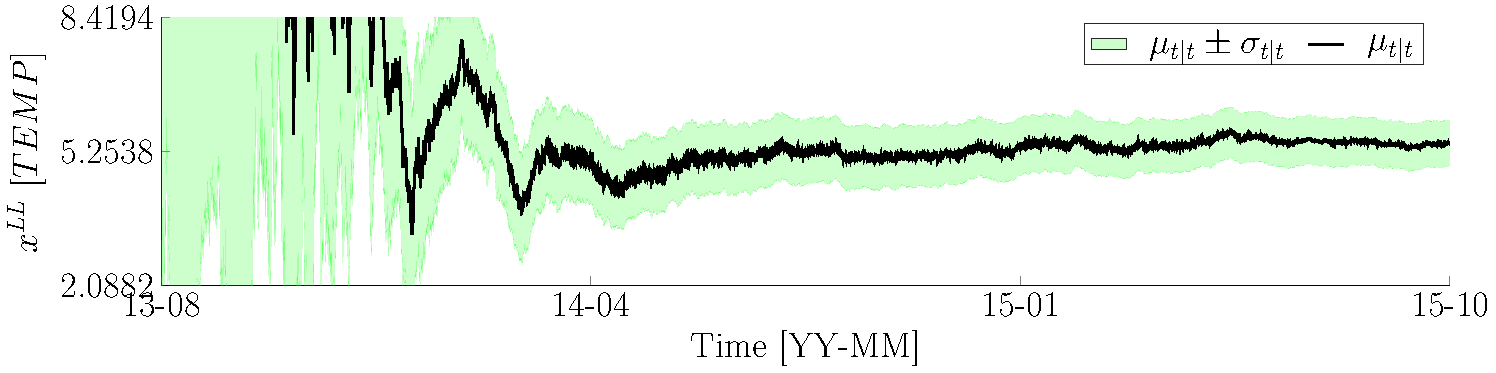
\includegraphics[width=0.9\linewidth]{./docfigs/Example_DISPTEMPSIM/optim_param_default_initialhiddenstate/TEMP_LL_1.pdf} 
%\caption{Estimated temperature local level component.}
%\end{subfigure}
%\begin{subfigure}{\linewidth}
%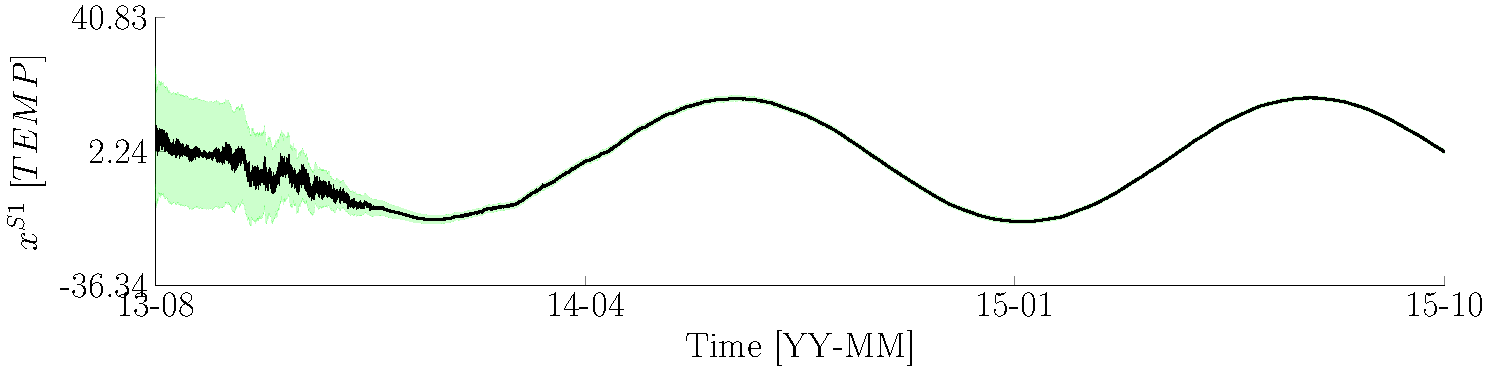
\includegraphics[width=0.9\linewidth]{./docfigs/Example_DISPTEMPSIM/optim_param_default_initialhiddenstate/TEMP_S1_2.pdf} 
%\caption{Estimated temperature yearly component (first hidden state)}
%\end{subfigure}
%\begin{subfigure}{\linewidth}
%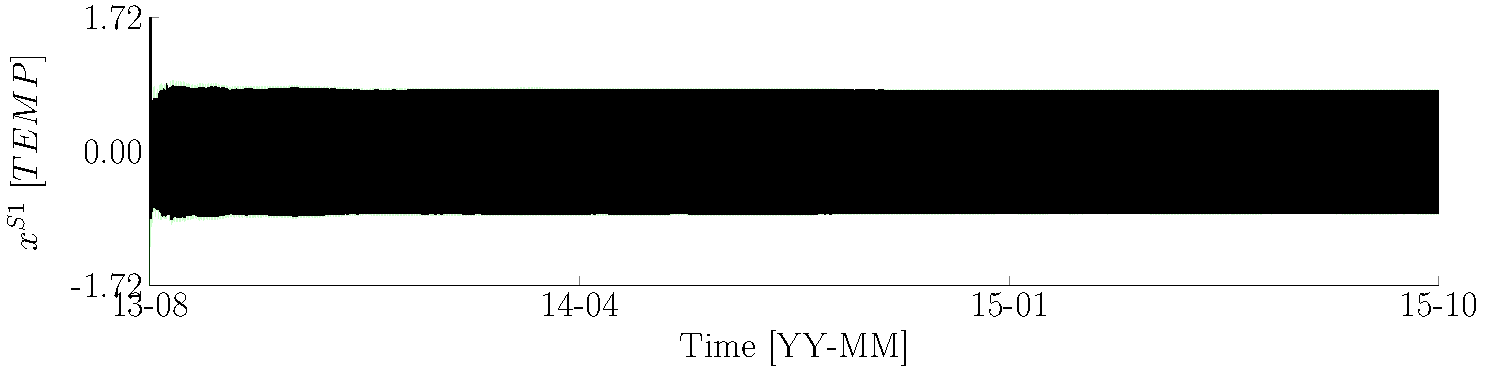
\includegraphics[width=0.9\linewidth]{./docfigs/Example_DISPTEMPSIM/optim_param_default_initialhiddenstate/TEMP_S1_4.pdf} 
%\caption{Estimated temperature daily component (first hidden state)}
%\end{subfigure}
%\begin{subfigure}{\linewidth}
%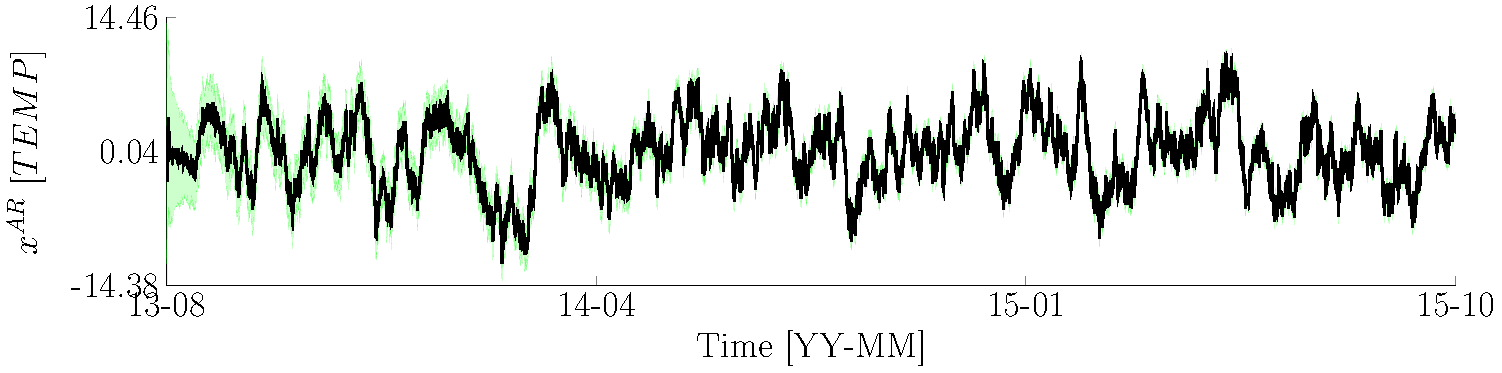
\includegraphics[width=0.9\linewidth]{./docfigs/Example_DISPTEMPSIM/optim_param_default_initialhiddenstate/TEMP_AR_6.pdf} 
%\caption{Estimated temperature autoregressive component}
%\end{subfigure}
%\caption{Estimated results using OpenBDLM optimized model parameters and default initial hidden states. The hidden states are estimated from the data presented in Figure~\ref{fig:DataSummaryDefaultPreProcessed2}a. The solid line and shaded area represent the mean and standard deviation of the estimated hidden states, respectively.}
%\label{fig:DISPTEMPSIMOptimizedDefaultExample2}
%\end{figure*}

\begin{figure*}[h!]
\centering
\begin{subfigure}{\linewidth}
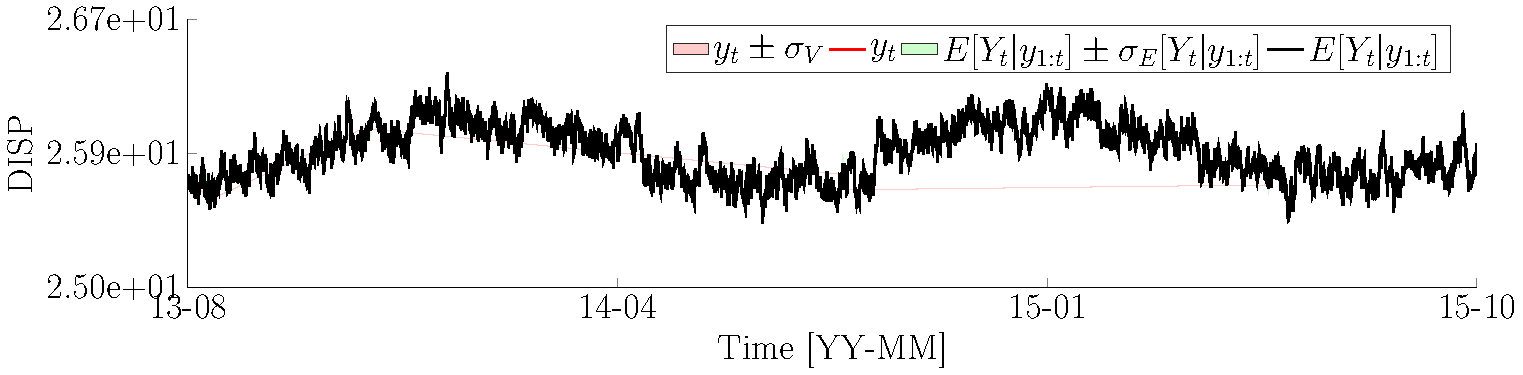
\includegraphics[width=0.9\linewidth]{./docfigs/Example_DISPTEMPSIM/optim_param_optim_initialhiddenstate/DISP_ObservedPredicted.pdf}
\caption{Observed and estimated displacement data} 
\end{subfigure}
\begin{subfigure}{\linewidth}
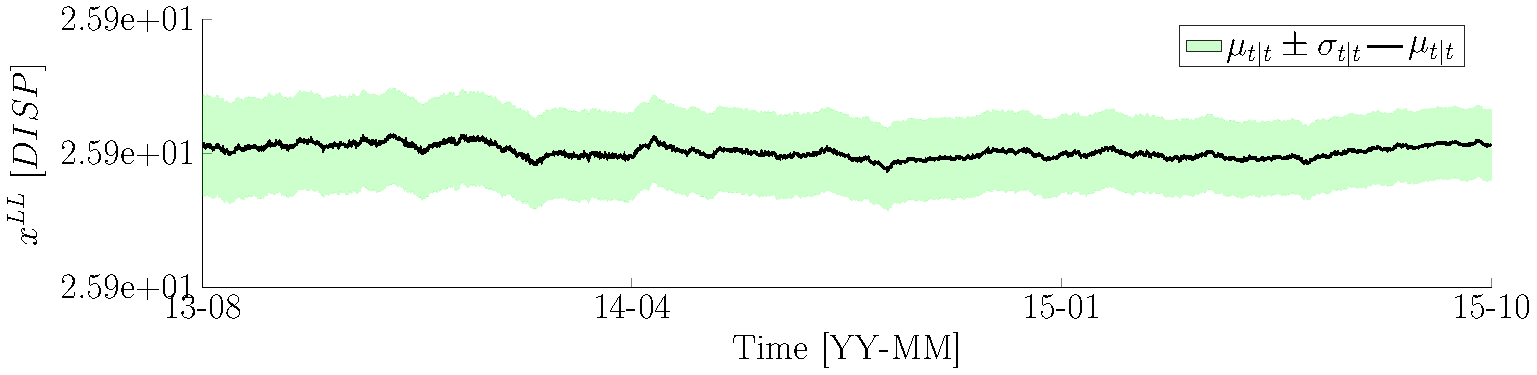
\includegraphics[width=0.9\linewidth]{./docfigs/Example_DISPTEMPSIM/optim_param_optim_initialhiddenstate/DISP_LL_1.pdf}
\caption{Estimated displacement local level component.}
\end{subfigure}
\begin{subfigure}{\linewidth}
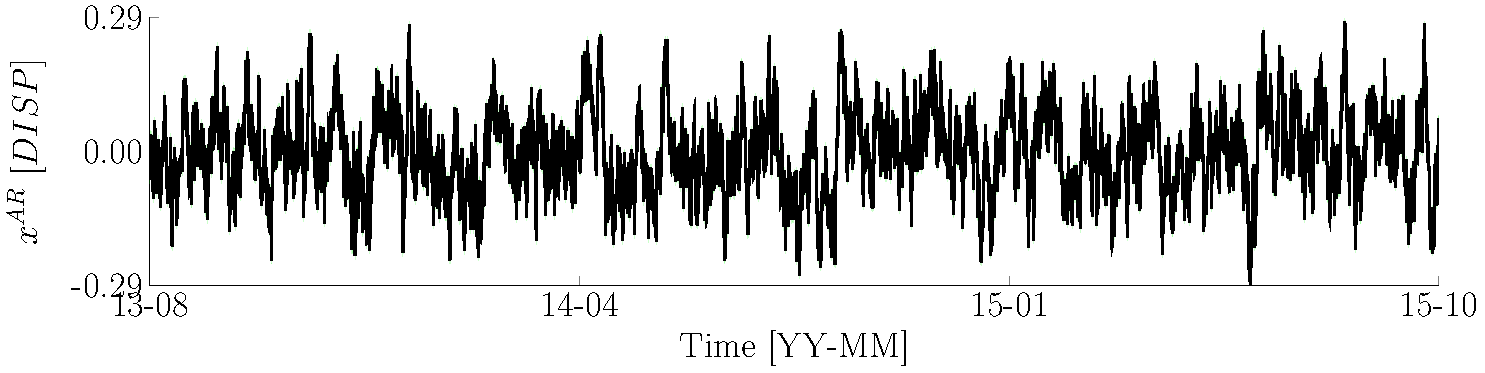
\includegraphics[width=0.9\linewidth]{./docfigs/Example_DISPTEMPSIM/optim_param_optim_initialhiddenstate/DISP_AR_2.pdf}
\caption{Estimated displacement autoregressive component.}
\end{subfigure}
\end{figure*}
\begin{figure*}[h!]
\ContinuedFloat
\begin{subfigure}{\linewidth}
\includegraphics[width=0.9\linewidth]{./docfigs/Example_DISPTEMPSIM/optim_param_optim_initialhiddenstate/TEMP_ObservedPredicted.pdf} 
\caption{Observed and estimated temperature data}
\end{subfigure}
\begin{subfigure}{\linewidth}
\includegraphics[width=0.9\linewidth]{./docfigs/Example_DISPTEMPSIM/optim_param_optim_initialhiddenstate/TEMP_LL_1.pdf} 
\caption{Estimated temperature local level component.}
\end{subfigure}
\begin{subfigure}{\linewidth}
\includegraphics[width=0.9\linewidth]{./docfigs/Example_DISPTEMPSIM/optim_param_optim_initialhiddenstate/TEMP_S1_2.pdf} 
\caption{Estimated temperature yearly component (first hidden state)}
\end{subfigure}
\begin{subfigure}{\linewidth}
\includegraphics[width=0.9\linewidth]{./docfigs/Example_DISPTEMPSIM/optim_param_optim_initialhiddenstate/TEMP_S1_4.pdf} 
\caption{Estimated temperature daily component (first hidden state)}
\end{subfigure}
\begin{subfigure}{\linewidth}
\includegraphics[width=0.9\linewidth]{./docfigs/Example_DISPTEMPSIM/optim_param_optim_initialhiddenstate/TEMP_AR_6.pdf} 
\caption{Estimated temperature autoregressive component}
\end{subfigure}
\caption{Estimated results using OpenBDLM optimized model parameters and optimized initial hidden states. The hidden states are estimated from the data presented in Figure~\ref{fig:DataSummaryDefaultPreProcessed2}a. The solid line and shaded area represent the mean and standard deviation of the estimated hidden states, respectively.}
\label{fig:DISPTEMPSIMOptimizedOptimizedExample2}
\end{figure*}\clearpage

\section{Step-by-step example: time-series with anomaly}
\label{S:ExampleDispAnomaly}

This example uses a single synthetic time series data that mimics displacement data measured on a bridge. 
The baseline switches between a trend stationary to acceleration stationary dynamics during a specific time window to mimic a fictitious anomaly.
The anomalous time windows is of 26 days duration, starting on June 25, 2010.


\subsection{Step 1: start a project}

First, choose the interactive tool by typing \colorbox{light-gray}{\lstinline[basicstyle = \mlttfamily \small, backgroundcolor = \color{light-gray}]!0!}.
Secondly, provide a project name (i.e. \lstinline[basicstyle = \mlttfamily \small, backgroundcolor = \color{light-gray}]!DISP_ANOMALY!).
Then, answer \colorbox{light-gray}{\lstinline[basicstyle = \mlttfamily \small, backgroundcolor = \color{light-gray}]!no!} to indicate that you are not concerned with creating synthetic data.
The next step is to type \colorbox{light-gray}{\lstinline[basicstyle = \mlttfamily \small, backgroundcolor = \color{light-gray}]!0!} to indicate that you aim to load new data.


\subsection{Step 2: load the data}

\begin{figure*}[h!]
\centering
\begin{subfigure}{\linewidth}
\includegraphics[width=0.9\linewidth]{./docfigs/Example_DISPSIM_ANOMALY/raw/ALL_AMPLITUDES.pdf} 
\caption{Amplitude}
\end{subfigure}
\begin{subfigure}{\linewidth}
\includegraphics[width=0.9\linewidth]{./docfigs/Example_DISPSIM_ANOMALY/raw/ALL_TIMESTEPS.pdf}
\caption{Timestep}
\end{subfigure}
\begin{subfigure}{\linewidth}
\includegraphics[width=0.9\linewidth]{./docfigs/Example_DISPSIM_ANOMALY/raw/AVAILABILITY.pdf}
\caption{Availability}
\end{subfigure}
\caption{Data used in Section~\ref{S:ExampleDispAnomaly}}.
\label{fig:DataSummaryRaw3}
\end{figure*}


At this stage, a graphical user interface should appear on screen. 
Browse the ``data/csv'' folder to select the csv file named \lstinline[basicstyle = \mlttfamily \small, backgroundcolor = \color{light-gray}]!DISP_ANOMALY_DISP.csv!.
Then, click on the Add button, and then the Done button, as highlighted in Figure~\ref{fig:DataLoadingUIPickFileExample1}.
You will notice that some basic information regarding the loaded time-series, such as the time series index, the reference name and the number of data points are now displayed in the \MATLAB{} command window.
At this time, three \MATLAB{} figures as those represented in Figure~\ref{fig:DataSummaryRaw3} should popup on screen.
The first figure represents in red the data amplitude of each time series data; the second figure represents the data timestep, and the last figure the data availability.
The figures show that data points exist between May 2008 and April 2012 (see Figure~\ref{fig:DataSummaryRaw3}a).
The timestep is non-uniform; it varies from 1 hour to 10 days (see Figure~\ref{fig:DataSummaryRaw3}b). 
The most frequent (i.e referent) time step is 12 hour.
There is no missing data on the displacement time-series.

\subsection{Step 4: configure the model}

First, the program requests the number of model class.
In this example, a change is clearly observed in the data, and we are therefore interested to model non-stationary data and eventually detect the change (i.e. anomaly detection).
In such case, we type \colorbox{light-gray}{\lstinline[basicstyle = \mlttfamily \small, backgroundcolor = \color{light-gray}]!2!} to build a switching model with two model classes.
Then, OpenBDLM asks for the type of block component for the first and second model class. 
The data baseline looks level or trend stationary, and there is a clear yearly periodic pattern superimposed to it.
%The presence of a daily periodic pattern is unclear.
Therefore, we choose \colorbox{light-gray}{\lstinline[basicstyle = \mlttfamily \small, backgroundcolor = \color{light-gray}]![23 31 41]!} for the first model class and \colorbox{light-gray}{\lstinline[basicstyle = \mlttfamily \small, backgroundcolor = \color{light-gray}]![13 31 41]!} for the second model class.
This model considers a trend stationary model with a yearly periodic pattern for the first model class, and an acceleration stationary model with a yearly periodic pattern for the second model class.
The next step is to define the model parameter constrain between the two model classes. 
Here, it is reasonable to consider that the two model classes only differs in the baseline dynamics, not in the periodic or autoregressive component. 
Therefore, we type \colorbox{light-gray}{\lstinline[basicstyle = \mlttfamily \small, backgroundcolor = \color{light-gray}]![0 1 1]!} to indicate that the two model classes share the same model parameter, except for the baseline component.
The  output on \MATLAB{} command window during interactive model configuration is presented in Listing~\ref{LST:OpenBDLMModelConfigureExample3}.
Type $\dlsh$ to valid.
The model is then built, a \lstinline[basicstyle = \mlttfamily \small, backgroundcolor = \color{light-gray}]!DATA_DISP_ANOMALY.mat! binary data file, a \lstinline[basicstyle = \mlttfamily \small, backgroundcolor = \color{light-gray}]!CFG_DISP_ANOMALY.m! configuration file, as well as a \lstinline[basicstyle = \mlttfamily \small, backgroundcolor = \color{light-gray}]!PROJ_DISP_ANOMALY.mat! project file are created.
The OpenBLDM main menu must appear on the \MATLAB{} command window (see Listing~\ref{LST:OpenBDLMMainMenu}).
Type \colorbox{light-gray}{\lstinline[basicstyle = \mlttfamily \small, backgroundcolor = \color{light-gray}]!Q!} to save and quit.



 \begin{lstlisting}[ frame = single, basicstyle = \mlttfamily \small, caption = { \MATLAB{} command window output during model configuration}, label = LST:OpenBDLMModelConfigureExample3,  float =h!, linewidth=\linewidth, captionpos=b, breaklines=true]
- How many model classes do you want for each time-series? 
     choice >> 2
     
     --------------------------------
     BDLM Component reference numbers
     --------------------------------
     11: Local level 
     12: Local trend 
     13: Local acceleration 
     21: Local level compatible with local trend 
     22: Local level compatible with local acceleration 
     23: Local trend compatible with local acceleration 
     31: Periodic 
     41: Autoregressive process (AR(1)) 
     51: Kernel regression 
     61: Level Intervention 
     --------------------------------

- Model class # 1 

- Identify components for time series #1; e.g. [11 31 41]
     choice >> [23 31 41]

- Model class # 2 

- Identify components for time series #1; e.g. [11 31 41]
     choice >> [13 31 41]

- Identify the shared parameters between the components of the model classes 1 and 2 for time  series #1 ; e.g. [0 1 1]
     choice >> [0 1 1]

     Building model...
     Saving project...
     Project saved in saved_projects/PROJ_DISP_ANOMALY.mat. 
     Printing configuration file...
     Saving data...

     Database saved in data/mat/DATA_DISP_ANOMALY.mat 
     Configuration file saved in config_files/CFG_DISP_ANOMALY.m. 
\end{lstlisting}



\subsection{Step 5: open the configuration file}

After the data loading and the model configuration, a configuration file named \lstinline[basicstyle = \mlttfamily \small, backgroundcolor = \color{light-gray}]!CFG_DISP_ANOMALY.m! configuration file is automatically created and saved in ``config\_files'' folder.
Open the configuration file from \MATLAB{} command line by typing  \colorbox{light-gray}{\lstinline[basicstyle = \mlttfamily \small, backgroundcolor = \color{light-gray}]!edit CFG_DISP_ANOMALY.m!}.
The Model parameters section of the configuration file shows that the model totalizes 12 model parameters, that is 
\begin{gather*}
\bm\theta=\{\sigma_{w, \text{D}}^{TcA,1}, p^{\text{PD1}}_{\text{D}}, \sigma_{w,\text{D}}^{\text{PD1}}, \phi^{AR}_{\text{D}}, \sigma_{w,\text{D}}^{AR}, \\
 \sigma_{w, \text{D}}^{LA,2}, \sigma_{w, \text{D}}^{TcA, 12}, \sigma_{w, \text{D}}^{LA, 21}, \sigma^{1}_{v,\text{D}}, \sigma^{2}_{v,\text{D}}, Z^{11},   Z^{22}\} 
 \end{gather*}
%The default value of the model parameters are assigned  using heuristic knowledge or computed from the data using statistics on the data.
The default model parameters values are 
\begin{gather*}
\bm\theta^{\text{default}}=\{1.5018\times10^{-8}, 365.24, 0, 0.75, 0.075092, \\
1.5018.10^{-8}, 1.5018\times10^{-8}, 1.5018\times10^{-5}, 0.075092, 0.075092, 0.99986, 0.99986\}.
\end{gather*}
%In the same manner, default value for the initial hidden states are assigned using heuristic knowledge or computed using statistics on the data.
The default initial hidden states mean, covariance  and model probability values for model class 1 are 
\begin{align*}
 \bm \mu^{1,\text{default}}_{0} & = [	-9.69, 	0,     	0,     	1,     	0,     	0        ]^{\intercal}, \text{and} \\
 \text{diag}(\bm\Sigma^{1,\text{default}}_{0})  & = [	18.2,  	4.56 , 	4.56  ,	18.2  ,	18.2  ,	4.56     ], \text{and} \\
 \pi_{0}^{1,\text{default}} & = 0.5.
\end{align*}
respectively.
The default initial hidden states mean, covariance  and model probability values for model class 2 are 
\begin{align*}
 \bm \mu^{2,\text{default}}_{0} & = [	-9.69, 	0,     	0,     	1,     	0,     	0        ]^{\intercal}, \text{and} \\
 \text{diag}(\bm\Sigma^{2,\text{default}}_{0})  & = [	18.2,  	4.56 , 	4.56  ,	18.2  ,	18.2  ,	4.56     ], \text{and} \\
 \pi_{0}^{2,\text{default}} & = 0.5.
\end{align*}
respectively.



\subsection{Step 6: estimate the hidden states}

Type \colorbox{light-gray}{\lstinline[basicstyle = \mlttfamily \small, backgroundcolor = \color{light-gray}]!OpenBDLM_main('CFG_DISP_ANOMALY.m');!} in the \MATLAB{} command line.
Once, the main menu appears, type  \colorbox{light-gray}{\lstinline[basicstyle = \mlttfamily \small, backgroundcolor = \color{light-gray}]!3!}, then \colorbox{light-gray}{\lstinline[basicstyle = \mlttfamily \small, backgroundcolor = \color{light-gray}]!1!} to estimate the filtered hidden states using the default model parameters and default initial hidden states values.
The value of the log-likelihood is $-409$.
The estimated hidden states are presented in Figure~\ref{fig:DISPSIMANOMALYDefaultDefaultExample3}.

\begin{figure*}[h!]
\centering
\begin{subfigure}{\linewidth}
\includegraphics[width=0.9\linewidth]{./docfigs/Example_DISPSIM_ANOMALY/default/DISP_ObservedPredicted.pdf}
\caption{Observed and estimated displacement data}
\end{subfigure}
\begin{subfigure}{\linewidth}
\includegraphics[width=0.9\linewidth]{./docfigs/Example_DISPSIM_ANOMALY/default/ModelProbability.pdf} 
\caption{Estimated probability of anomaly (probability of model class 2)}
\end{subfigure}
\begin{subfigure}{\linewidth}
\includegraphics[width=0.9\linewidth]{./docfigs/Example_DISPSIM_ANOMALY/default/DISP_LL_1.pdf} 
\caption{Estimated displacement local level component}
\end{subfigure}
\begin{subfigure}{\linewidth}
\includegraphics[width=0.9\linewidth]{./docfigs/Example_DISPSIM_ANOMALY/default/DISP_LT_2.pdf}
\caption{Estimated displacement local trend component.}
\end{subfigure}
\begin{subfigure}{\linewidth}
\includegraphics[width=0.9\linewidth]{./docfigs/Example_DISPSIM_ANOMALY/default/DISP_LAc_3.pdf}
\caption{Estimated displacement local acceleration component.}
\end{subfigure}
\end{figure*}
\begin{figure*}[h!]
\ContinuedFloat
\begin{subfigure}{\linewidth}
\includegraphics[width=0.9\linewidth]{./docfigs/Example_DISPSIM_ANOMALY/default/DISP_S1_4.pdf}
\caption{Estimated displacement yearly periodic component (first hidden state)}
\end{subfigure}
\begin{subfigure}{\linewidth}
\includegraphics[width=0.9\linewidth]{./docfigs/Example_DISPSIM_ANOMALY/default/DISP_AR_6.pdf} 
\caption{Estimated displacement autoregressive component}
\end{subfigure}
\caption{Estimated results using OpenBDLM default model parameters and default initial hidden states. The hidden states are estimated from the data presented in Figure~\ref{fig:DataSummaryRaw3}a. The solid line and shaded area represent the mean and standard deviation of the estimated hidden states, respectively.}
\label{fig:DISPSIMANOMALYDefaultDefaultExample3}
\end{figure*}

\subsection{Step 7: estimate the model parameters from the data}

Type \colorbox{light-gray}{\lstinline[basicstyle = \mlttfamily \small, backgroundcolor = \color{light-gray}]!OpenBDLM_main('CFG_DISP_ANOMALY.m');!} in the \MATLAB{} command line.
Once, the main menu appears, type  \colorbox{light-gray}{\lstinline[basicstyle = \mlttfamily \small, backgroundcolor = \color{light-gray}]!1!}, then \colorbox{light-gray}{\lstinline[basicstyle = \mlttfamily \small, backgroundcolor = \color{light-gray}]!1!} to estimate the model parameters using Newton-Raphson (type  \colorbox{light-gray}{\lstinline[basicstyle = \mlttfamily \small, backgroundcolor = \color{light-gray}]!1!} to use the Stochastic Gradient instead).
The model parameters learning procedure should start (see for example Listing~\ref{LST:OpenBLDMModelParameterLearning}).
Note that, by default, OpenBDLM considers that the parameters $PD1$, $\sigma_{w}^{PD1}$ are known.
Therefore, there are ten model parameters to be learned from the data in this example.
The estimation of the model parameters may take several hours.
Once the algorithm converged, the optimized model parameters values should be close to  \footnote{Note that it is possible to get slightly different value of parameters with the same performance.}
\begin{gather*}
\bm\theta^{\text{*}}=\{0, 365.24, 0, 0.75, 0.213, \\
0.001, 8.1224.10^{-6}, 1.5018\times10^{-5}, 0.10671, 0.10671, 0.99997, 0.99957\}.
\end{gather*}


\subsection{Step 8: estimate the hidden states using the optimized model parameters values}

Type \colorbox{light-gray}{\lstinline[basicstyle = \mlttfamily \small, backgroundcolor = \color{light-gray}]!OpenBDLM_main('CFG_DISP_ANOMALY_optim.m');!} in the \MATLAB{} command line to load the configuration file  \lstinline[basicstyle = \mlttfamily \small, backgroundcolor = \color{light-gray}]!CFG_DISP_ANOMALY_optim.m'!.
 \lstinline[basicstyle = \mlttfamily \small, backgroundcolor = \color{light-gray}]!CFG_DISP_ANOMALY_optim.m'! contains optimized model parameters previously estimated using the Newton-Raphson algorithm.
Once the main menu appears, type  \colorbox{light-gray}{\lstinline[basicstyle = \mlttfamily \small, backgroundcolor = \color{light-gray}]!3!}, then \colorbox{light-gray}{\lstinline[basicstyle = \mlttfamily \small, backgroundcolor = \color{light-gray}]!1!} to estimate the filtered hidden states using the optimized model parameters and default initial hidden states values.
The value of the log-likelihood is now $172$.
The estimated hidden states are presented in Figure~\ref{fig:DISPSIMANOMALYOptimizedDefaultExample3}.


\begin{figure*}[h!]
\centering
\begin{subfigure}{\linewidth}
\includegraphics[width=0.9\linewidth]{./docfigs/Example_DISPSIM_ANOMALY/optim_param_default_initialhiddenstate/DISP_ObservedPredicted.pdf}
\caption{Observed and estimated displacement data}
\end{subfigure}
\begin{subfigure}{\linewidth}
\includegraphics[width=0.9\linewidth]{./docfigs/Example_DISPSIM_ANOMALY/optim_param_default_initialhiddenstate/ModelProbability.pdf} 
\caption{Estimated probability of anomaly (probability of model class 2)}
\end{subfigure}
\begin{subfigure}{\linewidth}
\includegraphics[width=0.9\linewidth]{./docfigs/Example_DISPSIM_ANOMALY/optim_param_default_initialhiddenstate/DISP_LL_1.pdf} 
\caption{Estimated displacement local level component}
\end{subfigure}
\begin{subfigure}{\linewidth}
\includegraphics[width=0.9\linewidth]{./docfigs/Example_DISPSIM_ANOMALY/optim_param_default_initialhiddenstate/DISP_LT_2.pdf}
\caption{Estimated displacement local trend component.}
\end{subfigure}
\begin{subfigure}{\linewidth}
\includegraphics[width=0.9\linewidth]{./docfigs/Example_DISPSIM_ANOMALY/optim_param_default_initialhiddenstate/DISP_LAc_3.pdf}
\caption{Estimated displacement local acceleration component.}
\end{subfigure}
\end{figure*}
\begin{figure*}[h!]
\ContinuedFloat
\begin{subfigure}{\linewidth}
\includegraphics[width=0.9\linewidth]{./docfigs/Example_DISPSIM_ANOMALY/optim_param_default_initialhiddenstate/DISP_S1_4.pdf}
\caption{Estimated displacement yearly periodic component (first hidden state)}
\end{subfigure}
\begin{subfigure}{\linewidth}
\includegraphics[width=0.9\linewidth]{./docfigs/Example_DISPSIM_ANOMALY/optim_param_default_initialhiddenstate/DISP_AR_6.pdf} 
\caption{Estimated displacement autoregressive component}
\end{subfigure}
\caption{Estimated results using OpenBDLM optimized model parameters and default initial hidden states. The hidden states are estimated from the data presented in Figure~\ref{fig:DataSummaryRaw3}a. The solid line and shaded area represent the mean and standard deviation of the estimated hidden states, respectively.}
\label{fig:DISPSIMANOMALYOptimizedDefaultExample3}
\end{figure*}


\subsection{Step 9: estimate the initial hidden states}


Type \colorbox{light-gray}{\lstinline[basicstyle = \mlttfamily \small, backgroundcolor = \color{light-gray}]!OpenBDLM_main('CFG_DISPANOMALY_optim.m');!} in the \MATLAB{} command line.
Then, type  \colorbox{light-gray}{\lstinline[basicstyle = \mlttfamily \small, backgroundcolor = \color{light-gray}]!2!}, to optimize the initial hidden states value.
The optimized initial hidden states mean, covariance  and model probability values for model class 1 are 
\begin{align*}
 \bm \mu^{1,\text{*}}_{0} & = [	-9.4,  	-0.0115,	-7.39\times10^{-9},	1.06  ,	-0.00572	, -0.57     ]^{\intercal}, \text{and} \\
 \text{diag}(\bm\Sigma^{1,\text{default}}_{0})  & = [	0.147 ,	0.00093,	4.56 , 	0.00172,	0.000963	0.346      ],  \text{and} \\
 \pi_{0}^{1,\text{default}} & = 0.997,
\end{align*}
respectively.
The default initial hidden states mean, covariance  and model probability values for model class 2 are 
\begin{align*}
 \bm \mu^{2,\text{*}}_{0} & = [	9.54 	, 0.15  ,	-0.0966,	1.06  ,-0.00573, 	-0.486       ]^{\intercal}, \text{and} \\
 \text{diag}(\bm\Sigma^{2,\text{default}}_{0})  & = [	0.991 ,	0.722 ,	1.7  , 	0.00172	, 0.000963,	1.07     ], \text{and} \\
 \pi_{0}^{2,\text{default}} & = 0.00254,
\end{align*}
respectively.
Once it is done, type  \colorbox{light-gray}{\lstinline[basicstyle = \mlttfamily \small, backgroundcolor = \color{light-gray}]!2!}, and then  \colorbox{light-gray}{\lstinline[basicstyle = \mlttfamily \small, backgroundcolor = \color{light-gray}]!1!} to compute the filtered hidden states using the optimized model parameters and optimized initial hidden states.
The value of the log-likelihood is $188$.
The estimated hidden states are presented in Figure~\ref{fig:DISPSIMANOMALYOptimizedOptimizedExample3}.



\begin{figure*}[h!]
\centering
\begin{subfigure}{\linewidth}
\includegraphics[width=0.9\linewidth]{./docfigs/Example_DISPSIM_ANOMALY/optim_param_optim_initialhiddenstate/DISP_ObservedPredicted.pdf}
\caption{Observed and estimated displacement data}
\end{subfigure}
\begin{subfigure}{\linewidth}
\includegraphics[width=0.9\linewidth]{./docfigs/Example_DISPSIM_ANOMALY/optim_param_optim_initialhiddenstate/ModelProbability.pdf} 
\caption{Estimated probability of anomaly (probability of model class 2)}
\end{subfigure}
\begin{subfigure}{\linewidth}
\includegraphics[width=0.9\linewidth]{./docfigs/Example_DISPSIM_ANOMALY/optim_param_optim_initialhiddenstate/DISP_LL_1.pdf} 
\caption{Estimated displacement local level component}
\end{subfigure}
\begin{subfigure}{\linewidth}
\includegraphics[width=0.9\linewidth]{./docfigs/Example_DISPSIM_ANOMALY/optim_param_optim_initialhiddenstate/DISP_LT_2.pdf}
\caption{Estimated displacement local trend component.}
\end{subfigure}
\begin{subfigure}{\linewidth}
\includegraphics[width=0.9\linewidth]{./docfigs/Example_DISPSIM_ANOMALY/optim_param_optim_initialhiddenstate/DISP_LAc_3.pdf}
\caption{Estimated displacement local acceleration component.}
\end{subfigure}
\end{figure*}
\begin{figure*}[h!]
\ContinuedFloat
\begin{subfigure}{\linewidth}
\includegraphics[width=0.9\linewidth]{./docfigs/Example_DISPSIM_ANOMALY/optim_param_optim_initialhiddenstate/DISP_S1_4.pdf}
\caption{Estimated displacement yearly periodic component (first hidden state)}
\end{subfigure}
\begin{subfigure}{\linewidth}
\includegraphics[width=0.9\linewidth]{./docfigs/Example_DISPSIM_ANOMALY/optim_param_optim_initialhiddenstate/DISP_AR_6.pdf} 
\caption{Estimated displacement autoregressive component}
\end{subfigure}
\caption{Estimated results using OpenBDLM optimized model parameters and optimized initial hidden states. The hidden states are estimated from the data presented in Figure~\ref{fig:DataSummaryRaw3}a. The solid line and shaded area represent the mean and standard deviation of the estimated hidden states, respectively.}
\label{fig:DISPSIMANOMALYOptimizedOptimizedExample3}
\end{figure*}
\clearpage

\subsection{Example \#4: single time series analysis with non-harmonic periodic pattern}
\label{S:Example_TRAFFIC}
\subsubsection{Data description}

This case-study is conducted on the traffic loading data collected on the Tamar Bridge \citep{Goulet2017BDLMEmprical,Nguyen2019KRBDLM}. 
The Figure~\ref{fig:DataSummaryTraffic}a shows that data points exist between  September $01$ and October $21$, $2007$. Beyond that date, the timestamps are associated with \lstinline[basicstyle = \mlttfamily \small ]!NaN! (i.e. missing data) in order to forecast the predicted traffic load for a period of two weeks beyond the available data (see Figure~\ref{fig:DataSummaryTraffic}c).  
The timestep is $30$\,minutes for all data points (Figure~\ref{fig:DataSummaryTraffic}a).
The time series is stationnary with a level, a periodic pattern with a period of $7$\,days, and autoregressive pattern.
%The traffic loading on weekends is much lighter than those on weekdays. 
%For most of the day, the traffic load presents a high volume between $8$\,am and $4$\,pm, yet it drops out after $20$\,pm at night. 



\begin{figure*}[h]
\centering
\begin{subfigure}{\linewidth}\centering
\includegraphics[width=0.9\linewidth]{./docfigs/Example_TRAFFIC/raw/ALL_AMPLITUDES.pdf}
\caption{Amplitude}
\end{subfigure}
\begin{subfigure}{\linewidth}\centering
\includegraphics[width=0.9\linewidth]{./docfigs/Example_TRAFFIC/raw/ALL_TIMESTEPS.pdf} 
\caption{Timestep}
\end{subfigure}
\begin{subfigure}{\linewidth}\centering
\includegraphics[width=0.9\linewidth]{./docfigs/Example_TRAFFIC/raw/AVAILABILITY.pdf}
\caption{Availability}
\end{subfigure}
\caption{Data used in the example \#4.}
\label{fig:DataSummaryTraffic}
\end{figure*}


\subsubsection{Model description}
\label{SS:ModelConstructionExampleTraffic}

The model includes one model class, and the hidden states variables are 
\begin{gather*}
\begin{array}{rcl}
\mathbf{x} &=& \left[x^{\mathtt{LL}}, x_{0}^{\mathtt{KR}}, x_{1}^{\mathtt{KR}},\cdots,x_{100}^{\mathtt{KR}}, x^{\mathtt{AR}}\right]^{\intercal}.
\end{array}
\end{gather*}
The associated model parameters are
\begin{equation}
\label{EQ:PTL}
\bm\theta = \left[\sigma^{\mathtt{LL}}_{w}, \ell^{\mathtt{KR}}, p^{\mathtt{KR}}, \sigma_{w,0}^{\mathtt{KR}}, \sigma_{w,1}^{\mathtt{KR}}, \phi^{\mathtt{AR}}, \sigma^{\mathtt{AR}}_{w}, \sigma_{v}\right].
\end{equation}
The optimized model parameters values computed using the Newton-Raphson algorithm (see~\ref{SS:THModelParameterEstimation}) with a training period of 14 days are
\begin{gather*}
\bm\theta^{\text{*}}=[0 , 0.052, 7, 2.1\times10^{-5}, 0, 0.81, 0.30, 4.6\times10^{-5}].
\end{gather*}
The estimated initial hidden states mean and covariance are 
\begin{align*}
%\bm \mu^{*}_{0} & = [	 3.12  ,	0  ,   	-2.28  ,	-1.42  ,	-2.83 ,	-2.66 ,	-3    	,-2.68  \\
%&	-3.04 ,	-2.76 ,	-2.84 ,	-2.46 ,	-2.03 ,	-1.77 ,	-2.29 ,	-1.66  \\
%&	-2.81 ,	-1.12 ,	-3.01 ,	-2.38 ,	-2.94 ,	-2.14 ,	-4.11 ,	-0.562  \\
%&	-5.66 ,	4.08  ,	4.37  ,	2.45  ,	6.1   	2.23  ,	6.65  ,	0.261 ,	2.02  \\
%&	-3.09 ,	-2.05 ,	-1.01 ,	-3.75 ,	-1.3  	-3.71, 	0.13  ,	7.36  ,	1.01  \\
%&	7.83  ,	1.34  ,	6.47  ,	2.51  ,	1.08  ,	-1.13 ,	-3.78 	-0.0821,	-3.46  \\
%&	-2.67 ,	-1.99 ,	-3.81 ,	8.39  ,	0.615 ,	6.58  ,	2.37  	6.78  ,	2.88  \\
%&	1.27  ,	0.435 ,	-4.15 ,	-0.547,	-2.58 ,	-3.7 , 	-0.459	, -5.28  \\
%&	5.88  ,	2.47  ,	6.48  ,	4.43  ,	3.85  ,	6.17  ,	0.338 ,	1.41  \\
%&	-3.44 ,	-1.96 ,	-1.23 ,	-4.17 ,	-0.604,	-4.94 ,	2.38  ,	5.72  \\
%&	3.55  ,	5.32  ,	4.28  ,	4.23  ,	2.63  ,	-0.57 ,	-1.42 ,	-3.68  \\
%&	-0.623,	-4.01 ,	-1.72 ,	-3.56 ,	-1.27 ,	-1.42 ,	0.601 ,	-0.864	 \\
%& -0.961,	-1.48 ,	-0.109]^{\intercal}, \text{and} \\
\bm \mu^{*}_{0} & = [	 3.11  ,	0  ,   	-1.72  ,	-1.87 ,	\dots, -0.126]^{\intercal}, \text{and} \\
\bm\Sigma^{*}_{0} & = \text{diag}[   0.0828,	8.19,  	0.459, 	0.436 , \dots, 0.182 ].
 \end{align*}
The hidden states computed using the estimated model parameters and initial hidden states are presented in Figure~\ref{fig:Example_TrafficOptimizedOptimized}.









\subsubsection{Run the example from the pre-existing configuration file}
\label{SS:LoadConfigFileTraffic}


There is a configuration file CFG\_Example\_TRAFFIC\_optim.m which is located in the ``config\_files'' folder of the OpenBDLM package.
CFG\_Example\_TRAFFIC\_optim.m contains the optimized model parameters and initial hidden states values.
There is also a data file DATA\_Example\_TRAFFIC\_optim.mat that is located in the ``data/mat'' subfolder.
Therefore, it is possible to run the example \#4 by following the steps below while interacting with the \MATLAB{} command line:
\begin{enumerate}
\item Start OpenBDLM. Type \colorbox{light-gray}{\lstinline[basicstyle = \mlttfamily \small, backgroundcolor = \color{light-gray}]!OpenBDLM_main('CFG_Example_TRAFFIC_optim.m');!}.
\item Access hidden states estimation menu. Type \colorbox{light-gray}{\lstinline[basicstyle = \mlttfamily \small, backgroundcolor = \color{light-gray}]!3!}.
\item Run the Kalman filter to estimate the hidden states. Type \colorbox{light-gray}{\lstinline[basicstyle = \mlttfamily \small, backgroundcolor = \color{light-gray}]!1!}.
\item Save and quit. Type \colorbox{light-gray}{\lstinline[basicstyle = \mlttfamily \small, backgroundcolor = \color{light-gray}]!Q!}.
\end{enumerate}


\subsubsection{Run the example from command line interaction}

The analysis of a new dataset usually requires to start from scratch.
This section explains how to run the example \#4 from scratch, that is, how to load the data presented in Figure~\ref{fig:DataSummaryTraffic}, configure the model, estimate the model parameters and estimate the hidden states as presented in Figure~\ref{fig:Example_TrafficOptimizedOptimized}.
This may be done by following steps below while interacting with the \MATLAB{} command line:
\begin{enumerate}
\item Start OpenBDLM. Type \colorbox{light-gray}{\lstinline[basicstyle = \mlttfamily \small, backgroundcolor = \color{light-gray}]!OpenBDLM_main;!}.
\item Choose the interactive tool. Type \colorbox{light-gray}{\lstinline[basicstyle = \mlttfamily \small, backgroundcolor = \color{light-gray}]!0!}.
\item Enter the project name. Type \colorbox{light-gray}{\lstinline[basicstyle = \mlttfamily \small, backgroundcolor = \color{light-gray}]!Example_TRAFFIC!}. 
\item Disregard generating synthetic data. Type \colorbox{light-gray}{\lstinline[basicstyle = \mlttfamily \small, backgroundcolor = \color{light-gray}]!no!}. 
\item Load new data. Type \colorbox{light-gray}{\lstinline[basicstyle = \mlttfamily \small, backgroundcolor = \color{light-gray}]!0!}.
\item Select from the graphical user interface the data file Example\_TRAFFIC\_TrafficLoad.csv located in the folder ``/data/csv/Example\_TRAFFIC''. The Figure~\ref{fig:DataSummaryTraffic} representing the raw data should popup on screen.
\item Save and continue without pre-processing. Type \colorbox{light-gray}{\lstinline[basicstyle = \mlttfamily \small, backgroundcolor = \color{light-gray}]!7!}. The Figure~\ref{fig:DataSummaryTraffic} should popup on screen again,.
\item Select the number of model classes. Type \colorbox{light-gray}{\lstinline[basicstyle = \mlttfamily \small, backgroundcolor = \color{light-gray}]!1!}. 
\item Select the model block components. Type \colorbox{light-gray}{\lstinline[basicstyle = \mlttfamily \small, backgroundcolor = \color{light-gray}]![11 51 41]!}.
\item Access model parameters menu. Type \colorbox{light-gray}{\lstinline[basicstyle = \mlttfamily \small, backgroundcolor = \color{light-gray}]!11!}.
\item Modify a model parameter. Type \colorbox{light-gray}{\lstinline[basicstyle = \mlttfamily \small, backgroundcolor = \color{light-gray}]!1!}.
\item Modify the third model parameter (period of the kernel regression component). Type \colorbox{light-gray}{\lstinline[basicstyle = \mlttfamily \small, backgroundcolor = \color{light-gray}]!3!}.
\item Provide new value for  the period (in days). Type \colorbox{light-gray}{\lstinline[basicstyle = \mlttfamily \small, backgroundcolor = \color{light-gray}]!7!}.
\item Provide new bounds for the period. Type \colorbox{light-gray}{\lstinline[basicstyle = \mlttfamily \small, backgroundcolor = \color{light-gray}]![NaN NaN]!}.

\item Access the training period modification menu. Type \colorbox{light-gray}{\lstinline[basicstyle = \mlttfamily \small, backgroundcolor = \color{light-gray}]!13!}. 

\item Modify the training period. Type \colorbox{light-gray}{\lstinline[basicstyle = \mlttfamily \small, backgroundcolor = \color{light-gray}]!1!}. 

\item Choose the starting time (day). Type \colorbox{light-gray}{\lstinline[basicstyle = \mlttfamily \small, backgroundcolor = \color{light-gray}]!1!}. 

\item Choose the end time (day). Type \colorbox{light-gray}{\lstinline[basicstyle = \mlttfamily \small, backgroundcolor = \color{light-gray}]!14!}. 

\item Access model parameter estimation menu. Type \colorbox{light-gray}{\lstinline[basicstyle = \mlttfamily \small, backgroundcolor = \color{light-gray}]!1!}. 
\item Start Newton-Raphson algorithm. Type \colorbox{light-gray}{\lstinline[basicstyle = \mlttfamily \small, backgroundcolor = \color{light-gray}]!1!}. Once the algorithm has converged, the optimized model parameters values should be close to the values presented in Section~\ref{SS:ModelConstructionExampleTraffic}. Note that it is possible to get slightly different parameter values\footnote{Keep in mind that the optimization may take several minutes. It is possible to abort the analysis here and to load the configuration file called CFG\_Example\_TRAFFIC\_optim.m to load pre-computed values of model parameters, as presented in Section~\ref{SS:LoadConfigFileTraffic}.}.
\item Estimate the initial hidden states values. Type \colorbox{light-gray}{\lstinline[basicstyle = \mlttfamily \small, backgroundcolor = \color{light-gray}]!2!}.
\item Access hidden states estimation menu. Type \colorbox{light-gray}{\lstinline[basicstyle = \mlttfamily \small, backgroundcolor = \color{light-gray}]!3!}. 
\item Estimate the filtered hidden states. Type \colorbox{light-gray}{\lstinline[basicstyle = \mlttfamily \small, backgroundcolor = \color{light-gray}]!1!}. The estimation should correspond to the results presented in Figure~\ref{fig:Example_TrafficOptimizedOptimized}.
\item Access export menu. Type \colorbox{light-gray}{\lstinline[basicstyle = \mlttfamily \small, backgroundcolor = \color{light-gray}]!17!}. 
\item Export the current project in a configuration file. Type \colorbox{light-gray}{\lstinline[basicstyle = \mlttfamily \small, backgroundcolor = \color{light-gray}]!1!}.
\item Save and quit OpenBDLM. Type \colorbox{light-gray}{\lstinline[basicstyle = \mlttfamily \small, backgroundcolor = \color{light-gray}]!Q!}.
\end{enumerate}

\begin{figure*}[h!]
\begin{center}
\begin{subfigure}{\linewidth}\centering
\qquad~\includegraphics[width=0.83\linewidth]{./docfigs/Example_TRAFFIC/optim_param_optim_initialhiddenstate/TrafficLoad_ObservedPredicted.pdf} 
\caption{Observed and estimated traffic load data}
\end{subfigure}
\begin{subfigure}{\linewidth}\centering
\includegraphics[width=0.9\linewidth]{./docfigs/Example_TRAFFIC/optim_param_optim_initialhiddenstate/TrafficLoad_LL_1.pdf}
\caption{Estimated displacement local level component.}
\end{subfigure}
\begin{subfigure}{\linewidth}\centering
\includegraphics[width=0.9\linewidth]{./docfigs/Example_TRAFFIC/optim_param_optim_initialhiddenstate/TrafficLoad_KR0_2.pdf} 
\caption{Estimated traffic load yearly periodic component (first hidden state)}
\end{subfigure}
\begin{subfigure}{\linewidth}\centering
\includegraphics[width=0.9\linewidth]{./docfigs/Example_TRAFFIC/optim_param_optim_initialhiddenstate/TrafficLoad_KR1_3.pdf}
\caption{Estimated traffic load yearly periodic component (second hidden state)}
\end{subfigure}
\begin{subfigure}{\linewidth}\centering
\includegraphics[width=0.9\linewidth]{./docfigs/Example_TRAFFIC/optim_param_optim_initialhiddenstate/TrafficLoad_AR_4.pdf} 
\caption{Estimated traffic load autoregressive component}
\end{subfigure}
\caption{Estimated results using OpenBDLM with the optimized model parameters and optimized initial hidden states. The hidden states are estimated from the data presented in Figure~\ref{fig:DataSummaryTraffic}a. The solid line and shaded area represent the mean and standard deviation of the estimated hidden states, respectively.}
\label{fig:Example_TrafficOptimizedOptimized}
\end{center}
\end{figure*}

\clearpage

\subsection{Example \#5: single time series analysis with interventions}
\label{S:Example_DISP_intervention}
\subsubsection{Data description}
This case is based on Example \#1 (see \ref{S:Example_DISP}) where we removed some part of the data and introduce discrete shifts into it. This example illustrates what typically happens a sensor fails; when a sensor fails, the data start to be missing (i.e. \lstinline[basicstyle = \mlttfamily \small, backgroundcolor = \color{light-gray}]!NaN!) and it often takes from several weeks to several months before the sensor is replaced. When the sensor is replaced, it is in most cases re-initialized at a different initial value than the previous sensor which lead to a discrete shift in the time series, as depicted in Figure~\ref{fig:DataSummary1}. Here in addition to the components employed for Example \#1, we also employ a Local intervention in order to estimate the magnitude of the corrections require to eliminate the discrete shifts created by sensor replacement.

Note that again, in this example, we choose to resample the original data in order to have a timesteps of 6h instead of 1h. 

\begin{figure*}[h]
\centering
\begin{subfigure}{\linewidth}
\includegraphics[width=0.95\linewidth]{./docfigs/Example_DISP_INTERVENTION/ALL_AMPLITUDES.pdf}
\caption{Amplitude}
\end{subfigure}
\begin{subfigure}{\linewidth}
\centering
\includegraphics[width=0.9\linewidth]{./docfigs/Example_DISP_INTERVENTION/ALL_TIMESTEPS.pdf} 
\caption{Timestep}
\end{subfigure}
\begin{subfigure}{\linewidth}
\centering
\includegraphics[width=0.9\linewidth]{./docfigs/Example_DISP_INTERVENTION/AVAILABILITY.pdf}
\caption{Availability}
\end{subfigure}
\caption{Raw data in the example \#1 where the reference timestep is 1h.}
\label{fig:DataSummary1}
\end{figure*}


\subsubsection{Model description}
\label{SS:ModelConstructionExample1}
The model includes one model class, and the hidden states variables are 
\begin{gather*}
\textbf{x}=[x^{\mathtt{LL}}, x^{\mathtt{P1}\text{,yearly}}, x^{\mathtt{P2}\text{,yearly}}, x^{\mathtt{P1}\text{,daily}}, x^{\mathtt{P2}\text{,daily}}, x^{\mathtt{AR}}, x^{\mathtt{LI}}].
\end{gather*}
When using a Level intervention component, the user must provide discrete timestamps where it is required to estimate the magnitude of a discrete shift in the dataset (see \S\ref{SSS:LI}). A user can do so by specifying in the configuration file \colorbox{light-gray}{\lstinline[basicstyle = \mlttfamily \small, backgroundcolor = \color{light-gray}]!data.interventions=[t_{1}, t_{2}, ... , t_{n}]!}. The configuration file for this problem is presented in the Listing \ref{LST:CFGFileExampleInt} where the timestamps where the shift occur are \colorbox{light-gray}{\lstinline[basicstyle = \mlttfamily \small, backgroundcolor = \color{light-gray}]!data.interventions=[735929.875, 736099.875];!}. 

\begin{lstlisting}[linewidth=\linewidth, style=Matlab-editor,  basicstyle = \mlttfamily \tiny, backgroundcolor = \color{matlab-yellow}, caption = {Configuration file for the example \#5}, label=LST:CFGFileExampleInt, captionpos=b, float=h!]
%%%%%%%%%%%%%%%%%%%%%%%%%%%%%%%%%%%%%%%%%%%%%%%%%%%%%%%%%%%%%%%%%%%%%%%%%%%
%% A - Project name
%%%%%%%%%%%%%%%%%%%%%%%%%%%%%%%%%%%%%%%%%%%%%%%%%%%%%%%%%%%%%%%%%%%%%%%%%%%
misc.ProjectName='Example_DISP_INTERVENTION';
%%%%%%%%%%%%%%%%%%%%%%%%%%%%%%%%%%%%%%%%%%%%%%%%%%%%%%%%%%%%%%%%%%%%%%%%%%%
%% B - Data
%%%%%%%%%%%%%%%%%%%%%%%%%%%%%%%%%%%%%%%%%%%%%%%%%%%%%%%%%%%%%%%%%%%%%%%%%%%
dat=load('DATA_Example_DISP_INTERVENTION.mat'); 
data.values=dat.values;
data.timestamps=dat.timestamps;
data.labels={'DISP'};
data.interventions=[735929.875, 736099.875];
%%%%%%%%%%%%%%%%%%%%%%%%%%%%%%%%%%%%%%%%%%%%%%%%%%%%%%%%%%%%%%%%%%%%%%%%%%%
%% C - Model structure 
%%%%%%%%%%%%%%%%%%%%%%%%%%%%%%%%%%%%%%%%%%%%%%%%%%%%%%%%%%%%%%%%%%%%%%%%%%%
% Components reference numbers
% 11: Local level
% 12: Local trend
% 13: Local acceleration
% 21: Local level compatible with local trend
% 22: Local level compatible with local acceleration
% 23: Local trend compatible with local acceleration
% 31: Periodic
% 41: Autoregressive
% 51: Kernel regression
% 61: Level Intervention

% Model components
model.components.block{1}={[11 31 31 41 61 ] };
 
% Model inter-components dependence | {[components form dataset_i depends on components from  dataset_j]_i,[...]}
model.components.ic={[ ] };
%%%%%%%%%%%%%%%%%%%%%%%%%%%%%%%%%%%%%%%%%%%%%%%%%%%%%%%%%%%%%%%%%%%%%%%%%%%
%% D - Model parameters 
%%%%%%%%%%%%%%%%%%%%%%%%%%%%%%%%%%%%%%%%%%%%%%%%%%%%%%%%%%%%%%%%%%%%%%%%%%%
model.param_properties={
     % #1           #2             #3      #4    #5               #6           #7       #8              #9              #10
     % Param name   Block name     Model   Obs   Bound            Prior        Mean     Std             Values          Ref
     '\sigma_w',   'LL',           '1',   '1',   [NaN  NaN  ],    'N/A',       NaN,     NaN,            0,              1      %#1   
     'p',          'PD1',          '1',   '1',   [NaN  NaN  ],    'N/A',       NaN,     NaN,            365.2422,       2      %#2   
     '\sigma_w',   'PD1',          '1',   '1',   [NaN  NaN  ],    'N/A',       NaN,     NaN,            0,              3      %#3   
     'p',          'PD2',          '1',   '1',   [NaN  NaN  ],    'N/A',       NaN,     NaN,            1,              4      %#4   
     '\sigma_w',   'PD2',          '1',   '1',   [NaN  NaN  ],    'N/A',       NaN,     NaN,            0,              5      %#5   
     '\phi',       'AR',           '1',   '1',   [0  1      ],    'N/A',       NaN,     NaN,            0.90399,        6      %#6   
     '\sigma_w',   'AR',           '1',   '1',   [0  Inf    ],    'N/A',       NaN,     NaN,            0.035428,       7      %#7   
     '\mu_b',      'LI',           '1',   '1',   [NaN  NaN  ],    'N/A',       NaN,     NaN,            0,              8      %#8   
     '\sigma_b',   'LI',           '1',   '1',   [NaN  NaN  ],    'N/A',       NaN,     NaN,            0.16276,        9      %#9   
     '\sigma_v',   '',             '1',   '1',   [0  Inf    ],    'N/A',       NaN,     NaN,            6.193e-06,      10     %#10  
};
%%%%%%%%%%%%%%%%%%%%%%%%%%%%%%%%%%%%%%%%%%%%%%%%%%%%%%%%%%%%%%%%%%%%%%%%%%%
%% E - Initial states values 
%%%%%%%%%%%%%%%%%%%%%%%%%%%%%%%%%%%%%%%%%%%%%%%%%%%%%%%%%%%%%%%%%%%%%%%%%%%
% Initial hidden states mean for model 1:
model.initX{ 1 }=[	25.9  	-0.194	-0.01 	-0.00411	0.0551	-0.0127	0     ]';
% Initial hidden states variance for model 1: 
model.initV{ 1 }=diag([ 	8.26E-05	0.000143	0.000106	4.86E-07	4.86E-07	0.00167	1E-20  ]);
% Initial probability for model 1
model.initS{1}=[1     ];

\end{lstlisting}

The model parameters associated with this model are
\begin{gather*}
\bm\theta=[\sigma_{w}^{\mathtt{LL}}, p^{\mathtt{P}, \text{yearly}}, \sigma_{w}^{\mathtt{P}, \text{yearly}} , p^{\mathtt{P}, \text{daily}}, \sigma_{w}^{\mathtt{P}, \text{daily}}, \phi^{\mathtt{AR}}, \sigma_{w}^{\mathtt{AR}}, \mu_{b}^{\mathtt{LI}}, \sigma_{b}^{\mathtt{LI}}, \sigma_{v}].
\end{gather*}
The optimized model parameters values computed using the Newton-Raphson algorithm (see~\ref{SS:THModelParameterEstimation}) with a training period of 180 days  are
\begin{gather*}
\bm\theta^{\text{*}}=[0, 365.2422, 0, 1, 0, 0.903, 0.035, 0, 0.16 6.19\times10^{-6} ].
\end{gather*}
The estimated initial hidden states mean and covariance values are 
\begin{align*}
\bm \mu^{*}_{0} & = [	25.9,-0.194,-0.01	,-0.004,0.055,-0.013,0]^{\intercal}, \text{and} \\
\bm\Sigma^{*}_{0} & = \text{diag}([8.26\times10^{-5},	1.4\times10^{-4},	1.1\times10^{-4},	4.86\times10^{-7},	4.86\times10^{-7},	1.67\times10^{-3}  1E-20 ]).
 \end{align*}
The hidden states computed using the estimated model parameters and initial hidden states are presented in Figure~\ref{fig:Example_DISP_INTERVENTIONOptimizedOptimizedExample1}. You can see in Figure \ref{fig:Example_DISP_INTERVENTIONOptimizedOptimizedExample1}b that the level remains constant throughout the entire time series despite the jumps. This is because the discrete shift are estimated by the Level intervention component displayed in Figure \ref{fig:Example_DISP_INTERVENTIONOptimizedOptimizedExample1}e. 


\subsubsection{Run the example from the pre-existing configuration file}
\label{SS:LoadConfigFileEx1}
There is a configuration file CFG\_Example\_DISP\_INTERVENTION\_optim.m which is located in the ``config\_files'' folder of the OpenBDLM package.
CFG\_Example\_DISP\_INTERVENTION\_optim.m contains the optimized model parameters and estimated initial hidden states values (see Listing \ref{LST:CFGFileExampleInt}).
There is also a data file DATA\_Example\_DISP\_INTERVENTION\_optim.mat that is located in the ``data/mat'' subfolder.
Therefore, it is possible to run the example \#1 by following the steps below while interacting with the \MATLAB{} command line:
\begin{enumerate}
\item Start OpenBDLM. Type \colorbox{light-gray}{\lstinline[basicstyle = \mlttfamily \small, backgroundcolor = \color{light-gray}]!OpenBDLM_main('CFG_Example_DISP_INTERVENTION_optim.m');!}.
\item Access hidden states estimation menu. Type \colorbox{light-gray}{\lstinline[basicstyle = \mlttfamily \small, backgroundcolor = \color{light-gray}]!3!}.
\item Run the Kalman smoother to estimate the hidden states. Type \colorbox{light-gray}{\lstinline[basicstyle = \mlttfamily \small, backgroundcolor = \color{light-gray}]!1!}.
\item Save and quit. Type \colorbox{light-gray}{\lstinline[basicstyle = \mlttfamily \small, backgroundcolor = \color{light-gray}]!Q!}.
\end{enumerate}



\begin{figure*}[h!]
\begin{center}
\begin{subfigure}{\linewidth}
\centering
\includegraphics[width=0.9\linewidth]{./docfigs/Example_DISP_INTERVENTION/DISP_ObservedPredicted.pdf} 
\caption{Observed and estimated displacement data}
\end{subfigure}
\begin{subfigure}{\linewidth}
\centering
\includegraphics[width=0.9\linewidth]{./docfigs/Example_DISP_INTERVENTION/DISP_LL_1.pdf}
\caption{Estimated displacement local level component.}
\end{subfigure}
\begin{subfigure}{\linewidth}
\centering
\includegraphics[width=0.9\linewidth]{./docfigs/Example_DISP_INTERVENTION/DISP_S1_2.pdf} 
\caption{Estimated displacement yearly periodic component (first hidden state)}
\end{subfigure}
\begin{subfigure}{\linewidth}
\centering
\includegraphics[width=0.9\linewidth]{./docfigs/Example_DISP_INTERVENTION/DISP_AR_6.pdf} 
\caption{Estimated displacement autoregressive component}
\end{subfigure}
\begin{subfigure}{\linewidth}
\centering
\includegraphics[width=0.9\linewidth]{./docfigs/Example_DISP_INTERVENTION/DISP_LI_7.pdf}
\caption{Estimated displacement daily periodic component (first hidden state)}
\end{subfigure}
\caption{Estimated results using OpenBDLM with the optimized model parameters and estimated initial hidden states. The hidden states are estimated from the data presented in Figure~\ref{fig:DataSummary1}a. The solid line and shaded area represent the mean and standard deviation of the estimated hidden states.}
\label{fig:Example_DISP_INTERVENTIONOptimizedOptimizedExample1}
\end{center}
\end{figure*}



\clearpage

\subsection{Example \#5: generate and analyze synthetic data }
\label{S:EXAMPLESYNTHETICDATA}


\subsubsection{Purpose}
This example illustrates how to create a synthetic time series using OpenBDLM.
The objective is to create a 4-years long time series with an acceleration stationary baseline, and a yearly periodic pattern as well as a autoregressive process superimposed into it. 
The timestep is 1 day.
This example corresponds to the OpenBDLM demo presented in Section~\ref{S:OPENBDLMGETTINGSTARTED}.

\begin{figure*}[h!]
\centering
\begin{subfigure}{\linewidth}
\includegraphics[width=0.9\linewidth]{./docfigs/Example_SYNTHETIC/raw/ALL_AMPLITUDES.pdf} 
\caption{Amplitude}
\end{subfigure}
\begin{subfigure}{\linewidth}
\includegraphics[width=0.9\linewidth]{./docfigs/Example_SYNTHETIC/raw/ALL_TIMESTEPS.pdf}
\caption{Timestep}
\end{subfigure}
\begin{subfigure}{\linewidth}
\includegraphics[width=0.9\linewidth]{./docfigs/Example_SYNTHETIC/raw/AVAILABILITY.pdf}
\caption{Availability}
\end{subfigure}
\caption{Data used in example \#5}.
\label{fig:DataSummaryRawSynthetic}
\end{figure*}


\subsubsection{Model description}
The model includes one model class, and the block components are 
\begin{gather*}
\textbf{x}=[x^{\mathtt{LL}}, x^{\mathtt{LT}}, x^{\mathtt{La}}, x^{\mathtt{P1}\text{,yearly}}, x^{\mathtt{P2}\text{,yearly}}, x^{\mathtt{AR}}].
\end{gather*}
The associated model parameters are
\begin{gather*}
\bm\theta=\{\sigma_{w}^{\mathtt{LA}}, p^{\mathtt{PD}, \text{yearly}}, \sigma_{w}^{\mathtt{PD}, \text{yearly}}, \phi^{\mathtt{AR}}, \sigma_{w}^{\mathtt{AR}}, \sigma_{v,\text{D}}\} 
 \end{gather*}
The model parameters values assigned by default from OpenBDLM are
\begin{gather*}
\bm\theta^{\text{defaut}}=[ 1\times10^{-8}, 365.24, 0, 0.75, 0.01, 0.01].
\end{gather*}
The default initial hidden states mean and covariance values, and model probability are 
\begin{align*}
\bm \mu^{\text{defaut}}_{0} & = [	 10  , -1\times10^{-5}  ,	-0.001	,	10  ,  	10    ,	0  ]^{\intercal}, \text{and} \\
\bm\Sigma^{\text{defaut}}_{0} & = \text{diag}[ 0.01  ,	0.01  ,	0.01  	,0.04  ,	0.04  ,	0.01 ], \\
 \pi_{0}^{1,\text{default}} & = 1,
 \end{align*}
 respectively.
The synthetic data generated from this model structure, model parameters values and initial hidden states values are presented in Figure~\ref{fig:DataSummaryRawSynthetic}.
The hidden states computed using the same (i.e. true) model structure, model parameters values and initial hidden states values are presented in Figure~\ref{fig:SYNTHETICOptimizedOptimized}.

\subsubsection{Run the example from command line interaction}

This section explains how to run the example \#4, that is, how to generate the synthetic data presented in Figure~\ref{fig:DataSummaryRawSynthetic}, and estimate the hidden states as presented in Figure~\ref{fig:SYNTHETICOptimizedOptimized}.


\begin{enumerate}
\item Start OpenBDLM. Type \colorbox{light-gray}{\lstinline[basicstyle = \mlttfamily \small, backgroundcolor = \color{light-gray}]!OpenBDLM_main;!}.
\item Choose the interactive tool. Type \colorbox{light-gray}{\lstinline[basicstyle = \mlttfamily \small, backgroundcolor = \color{light-gray}]!0!}.
\item Enter the project name. Type \colorbox{light-gray}{\lstinline[basicstyle = \mlttfamily \small, backgroundcolor = \color{light-gray}]!Example_SYNTHETIC!}. 
\item Generate synthetic data. Type \colorbox{light-gray}{\lstinline[basicstyle = \mlttfamily \small, backgroundcolor = \color{light-gray}]!yes!}. 
\item Provide the number of time series. Type \colorbox{light-gray}{\lstinline[basicstyle = \mlttfamily \small, backgroundcolor = \color{light-gray}]!1!}.
\item Provide  the date corresponding of the first data sample. Type \colorbox{light-gray}{\lstinline[basicstyle = \mlttfamily \small, backgroundcolor = \color{light-gray}]!2000-01-01!}.
\item Provide  the date corresponding of the last data sample. Type \colorbox{light-gray}{\lstinline[basicstyle = \mlttfamily \small, backgroundcolor = \color{light-gray}]!2005-01-01!}.
\item Provide  the timestep in day. Type \colorbox{light-gray}{\lstinline[basicstyle = \mlttfamily \small, backgroundcolor = \color{light-gray}]!1!}.
\item Select the number of model classes. Type \colorbox{light-gray}{\lstinline[basicstyle = \mlttfamily \small, backgroundcolor = \color{light-gray}]!1!}. 
\item Select the model block components. Type \colorbox{light-gray}{\lstinline[basicstyle = \mlttfamily \small, backgroundcolor = \color{light-gray}]![13 31 41]!}. The Figure~\ref{fig:DataSummaryRawSynthetic} should popup on screen.
\item Access hidden states estimation menu. Type \colorbox{light-gray}{\lstinline[basicstyle = \mlttfamily \small, backgroundcolor = \color{light-gray}]!3!}. 
\item Estimate the filtered hidden states. Type \colorbox{light-gray}{\lstinline[basicstyle = \mlttfamily \small, backgroundcolor = \color{light-gray}]!1!}. The estimation should be similar to the results presented in Figure~\ref{fig:SYNTHETICOptimizedOptimized}.
\item Save and quit OpenBDLM. Type \colorbox{light-gray}{\lstinline[basicstyle = \mlttfamily \small, backgroundcolor = \color{light-gray}]!Q!}.
\end{enumerate}



%First, choose the interactive tool by typing \colorbox{light-gray}{\lstinline[basicstyle = \mlttfamily \small, backgroundcolor = \color{light-gray}]!0!}.
%Secondly, provide a project name (i.e. \lstinline[basicstyle = \mlttfamily \small, backgroundcolor = \color{light-gray}]!Example_SYNTHETIC!).
%Then, answer \colorbox{light-gray}{\lstinline[basicstyle = \mlttfamily \small, backgroundcolor = \color{light-gray}]!yes!} to indicate that you would like to create synthetic data.
%Finally, type \colorbox{light-gray}{\lstinline[basicstyle = \mlttfamily \small, backgroundcolor = \color{light-gray}]!1!} to create one single synthetic time series. 
%
%\subsection{Step 2: define the time step vector}
%
%Type \colorbox{light-gray}{\lstinline[basicstyle = \mlttfamily \small, backgroundcolor = \color{light-gray}]!2000-01-01!}, \colorbox{light-gray}{\lstinline[basicstyle = \mlttfamily \small, backgroundcolor = \color{light-gray}]!2005-01-01!} and \colorbox{light-gray}{\lstinline[basicstyle = \mlttfamily \small, backgroundcolor = \color{light-gray}]!1!}, to provide the date corresponding of the first and last data sample of the synthetic data, as well as the timestep in days.


%\subsection{Step 3: configure the model}
%
%First, the program requests the number of model class.
%In this example, we would like to create synthetic data with no anomaly.
%In such case, we type \colorbox{light-gray}{\lstinline[basicstyle = \mlttfamily \small, backgroundcolor = \color{light-gray}]!1!} to choose a single model class.
%Then, OpenBDLM asks for the type of block component.
%As mentionned earlier, the objective is to create synthetic time series data with an acceleration stationary baseline, and a yearly periodic pattern superimposed into it. 
%%The presence of a daily periodic pattern is unclear.
%Therefore, we choose \colorbox{light-gray}{\lstinline[basicstyle = \mlttfamily \small, backgroundcolor = \color{light-gray}]![13 31 41]!}.
%This model considers a trend stationary model with a yearly periodic pattern, and an autoregressive process to be more realistic.
%At this time, three figures  that represent the amplitude, timestep and availability of the newly created synthetic data (as shown in Figure~\ref{fig:DataSummaryRawSynthetic}) should popup on the screen.
%Type \colorbox{light-gray}{\lstinline[basicstyle = \mlttfamily \small, backgroundcolor = \color{light-gray}]!Q!} to save and quit.
%
%\subsection{Step 4: explore the model}
%From the main menu, type  \colorbox{light-gray}{\lstinline[basicstyle = \mlttfamily \small, backgroundcolor = \color{light-gray}]!11!} to see what are the values of model parameters which have been assigned to create the synthetic data.
%The model totalizes 6 model parameters, that is 
%\begin{gather*}
%\bm\theta=\{\sigma_{w, \text{D}}^{LA}, p^{\text{PD1}}_{\text{D}}, \sigma_{w,\text{D}}^{\text{PD1}}, \phi^{AR}_{\text{D}}, \sigma_{w,\text{D}}^{AR}, \sigma_{v,\text{D}}\} 
% \end{gather*}
%The default model parameters values are 
%\begin{gather*}
%\bm\theta^{\text{default}}=\{1\times10^{-8}, 365.24, 0, 0.75, 0.01, 0.01\}, 
%\end{gather*}
%in agreement with the values indicated in Table~\ref{table:defaultsynthetic}.
%Type \colorbox{light-gray}{\lstinline[basicstyle = \mlttfamily \small, backgroundcolor = \color{light-gray}]!R!} to return to the main menu.
%Then, type \colorbox{light-gray}{\lstinline[basicstyle = \mlttfamily \small, backgroundcolor = \color{light-gray}]!12!} the see that the default initial hidden states mean, covariance  and model probability values are 
%\begin{align*}
% \bm \mu^{1,\text{default}}_{0} & = [	10  , -1\times10^{-5}  ,	-0.001	,	10  ,  	10    ,	0         ]^{\intercal}, \text{and} \\
% \text{diag}(\bm\Sigma^{1,\text{default}}_{0})  & = [	0.01  ,	0.01  ,	0.01  	,0.04  ,	0.04  ,	0.01     ], \text{and} \\
% \pi_{0}^{1,\text{default}} & = 1.
%\end{align*}
%respectively, in agreement with the values indicated in Table~\ref{table:defaultsynthetic}.
%Type \colorbox{light-gray}{\lstinline[basicstyle = \mlttfamily \small, backgroundcolor = \color{light-gray}]!R!} to return to the main menu.

%\begin{figure*}[h!]
%\centering
%\begin{subfigure}{\linewidth}
%\includegraphics[width=0.9\linewidth]{./docfigs/Example_SYNTHETIC/raw/ALL_AMPLITUDES.pdf} 
%\caption{Amplitude}
%\end{subfigure}
%\begin{subfigure}{\linewidth}
%\includegraphics[width=0.9\linewidth]{./docfigs/Example_SYNTHETIC/raw/ALL_TIMESTEPS.pdf}
%\caption{Timestep}
%\end{subfigure}
%\begin{subfigure}{\linewidth}
%\includegraphics[width=0.9\linewidth]{./docfigs/Example_SYNTHETIC/raw/AVAILABILITY.pdf}
%\caption{Availability}
%\end{subfigure}
%\caption{Data used in example \#4}.
%\label{fig:DataSummaryRawSynthetic}
%\end{figure*}


%\subsection{Step 5: estimate the hidden states}
%
%From the main menu, type  \colorbox{light-gray}{\lstinline[basicstyle = \mlttfamily \small, backgroundcolor = \color{light-gray}]!3!}, then \colorbox{light-gray}{\lstinline[basicstyle = \mlttfamily \small, backgroundcolor = \color{light-gray}]!1!} to estimate the filtered hidden states using the default model parameters and default initial hidden states values.
%The value of the log-likelihood is $4976$, and the estimated hidden states are presented in Figure~\ref{fig:SYNTHETICDefaultDefaultExample4}.
%For each figure, the red dashed line represents the true known values of the hidden states.
%
%\begin{figure*}[h!]
%\centering
%\begin{subfigure}{\linewidth}
%\includegraphics[width=0.9\linewidth]{./docfigs/Example_SYNTHETIC/default/TS01_ObservedPredicted.pdf}
%\caption{Observed and estimated displacement data}
%\end{subfigure}
%\begin{subfigure}{\linewidth}
%\includegraphics[width=0.9\linewidth]{./docfigs/Example_SYNTHETIC/default/TS01_LL_1.pdf} 
%\caption{Estimated displacement local level component}
%\end{subfigure}
%\begin{subfigure}{\linewidth}
%\includegraphics[width=0.9\linewidth]{./docfigs/Example_SYNTHETIC/default/TS01_LT_2.pdf}
%\caption{Estimated displacement local trend component.}
%\end{subfigure}
%\begin{subfigure}{\linewidth}
%\includegraphics[width=0.9\linewidth]{./docfigs/Example_SYNTHETIC/default/TS01_LA_3.pdf}
%\caption{Estimated displacement local acceleration component.}
%\end{subfigure}
%\end{figure*}
%\begin{figure*}[h!]
%\ContinuedFloat
%\begin{subfigure}{\linewidth}
%\includegraphics[width=0.9\linewidth]{./docfigs/Example_SYNTHETIC/default/TS01_S1_4.pdf}
%\caption{Estimated displacement yearly periodic component (first hidden state)}
%\end{subfigure}
%\begin{subfigure}{\linewidth}
%\includegraphics[width=0.9\linewidth]{./docfigs/Example_SYNTHETIC/default/TS01_AR_6.pdf} 
%\caption{Estimated displacement autoregressive component}
%\end{subfigure}
%\caption{Estimated results using OpenBDLM default model parameters and default initial hidden states. The hidden states are estimated from the data presented in Figure~\ref{fig:DataSummaryRawSynthetic}a. The solid line and shaded area represent the mean and standard deviation of the estimated hidden states, respectively. The red dashed line represent the true the hidden state value.}
%\label{fig:SYNTHETICDefaultDefaultExample4}
%\end{figure*}

%\subsection{Step 6: estimate the initial hidden states}
%
%From the main menu, type  \colorbox{light-gray}{\lstinline[basicstyle = \mlttfamily \small, backgroundcolor = \color{light-gray}]!2!}, to optimize the initial hidden states value.
%The estimated initial hidden states mean and covariance values are 
%\begin{align*}
%\bm \mu^{*}_{0} & = [	10 ,   	-0.00103,	-9.68\times10^{-6},	10   , 	10    ,	-0.0106  ]^{\intercal}, \text{and} \\
% \text{diag}(\bm\Sigma^{*}_{0}) & = [	2.35\times10^{-5}	, 1.33\times10^{-9},	3.3\times10^{-14}	, 1.9\times10^{-6}	, 2.03\times10^{-6}	,0.000353    ], 
% \end{align*}
% respectively.
%Once it is done, type  \colorbox{light-gray}{\lstinline[basicstyle = \mlttfamily \small, backgroundcolor = \color{light-gray}]!3!}, and then  \colorbox{light-gray}{\lstinline[basicstyle = \mlttfamily \small, backgroundcolor = \color{light-gray}]!1!} to compute the filtered hidden states using the optimized model parameters and optimized initial hidden states.
%The value of the log-likelihood is $5011$.
%The estimated hidden states are presented in Figure~\ref{fig:SYNTHETICOptimizedOptimized}.


\begin{figure*}[h!]
\centering
\begin{subfigure}{\linewidth}
\includegraphics[width=0.9\linewidth]{./docfigs/Example_SYNTHETIC/optim_param_optim_initialhiddenstate/TS01_ObservedPredicted.pdf}
\caption{Observed and estimated displacement data}
\end{subfigure}
\begin{subfigure}{\linewidth}
\includegraphics[width=0.9\linewidth]{./docfigs/Example_SYNTHETIC/optim_param_optim_initialhiddenstate/TS01_LL_1.pdf} 
\caption{Estimated displacement local level component}
\end{subfigure}
\begin{subfigure}{\linewidth}
\includegraphics[width=0.9\linewidth]{./docfigs/Example_SYNTHETIC/optim_param_optim_initialhiddenstate/TS01_LT_2.pdf}
\caption{Estimated displacement local trend component.}
\end{subfigure}
\begin{subfigure}{\linewidth}
\includegraphics[width=0.9\linewidth]{./docfigs/Example_SYNTHETIC/optim_param_optim_initialhiddenstate/TS01_LA_3.pdf}
\caption{Estimated displacement local acceleration component.}
\end{subfigure}
\end{figure*}
\begin{figure*}[h!]
\ContinuedFloat
\begin{subfigure}{\linewidth}
\includegraphics[width=0.9\linewidth]{./docfigs/Example_SYNTHETIC/optim_param_optim_initialhiddenstate/TS01_S1_4.pdf}
\caption{Estimated displacement yearly periodic component (first hidden state)}
\end{subfigure}
\begin{subfigure}{\linewidth}
\includegraphics[width=0.9\linewidth]{./docfigs/Example_SYNTHETIC/optim_param_optim_initialhiddenstate/TS01_AR_6.pdf} 
\caption{Estimated displacement autoregressive component}
\end{subfigure}
\caption{Estimated results using OpenBDLM default model parameters and optimized initial hidden states. The hidden states are estimated from the data presented in Figure~\ref{fig:DataSummaryRawSynthetic}a. The solid line and shaded area represent the mean and standard deviation of the estimated hidden states, respectively. The red dashed line represent the true the hidden state value.}
\label{fig:SYNTHETICOptimizedOptimized}
\end{figure*}




\section{FAQ Troubleshooting}
%
%\begin{itemize}
%\item How to cite OpenBDLM ?\\
%
%\noindent \emph{OpenBDLM, an Open-Source Software for Structural Health Monitoring using Bayesian Dynamic Linear Models}\\{\small
%            Gaudot, I., Nguyen, L.H., Khazaeli S.and Goulet, J.-A.\\
%            Submitted to 13th International Conference on Applications of Statistics and Probability in Civil Engineering, Vol. X, Issue X, 2019\\}
%      [] [~]  [~] [] \cite{Gaudot2019OpenBDLM}\\[4pt]
%
%\end{itemize}

%
%\Que{Here first question would come}
%\Ans{\lipsum[1]\lipsum[1]}
%
%\Que{Here second question would come}
%\Ans{\lipsum[1]\lipsum[1]}


\begin{description}[style=unboxed]

\item[\textbf{The state estimation crashes. What can I do ?}] \leavevmode \\

There are two well-known issues that make the state estimation to crash.
\begin{itemize}
\item numerical instabilities of the Kalman computation due to missing data and/or non-uniform time step vector. Possible solution: switch to UD computation (see Section~\ref{S:HIDDENSTATESESTIMATION}). An alternative consists in removing missing data in the original data, and/or make the timestep vector uniform using the pre-processing tools (see Section~\ref{S:DATAEDITINGPREPROCESSING}).
\item pinv error. Possible solution: in the \lstinline[basicstyle = \mlttfamily \small ]!KalmanFilter.m! function, change the tolerance value of the built-in \MATLAB{} function  \lstinline[basicstyle = \mlttfamily \small ]!pinv.m!. See \url{https://www.mathworks.com/help/matlab/ref/pinv.html} for more details.
\end{itemize}

\item[\textbf{The model parameter estimation crashes. What can I do ?}] \leavevmode \\
This is likely due to the fact that the state estimation crashes. 
There are two well-known issues that make the state estimation to crash.
\begin{itemize}
\item numerical instabilities of the Kalman computation due to missing data and/or non-uniform time step vector. Possible solution: switch to UD computation (see Section~\ref{S:HIDDENSTATESESTIMATION}). An alternative consists in removing missing data in the original data, and/or make the timestep vector uniform using the pre-processing tools (see Section~\ref{S:DATAEDITINGPREPROCESSING}).
\item pinv error. Possible solution: in the \lstinline[basicstyle = \mlttfamily \small ]!KalmanFilter.m! function, change the tolerance value of the built-in \MATLAB{} function  \lstinline[basicstyle = \mlttfamily \small ]!pinv.m!. See \url{https://www.mathworks.com/help/matlab/ref/pinv.html} for more details.
\end{itemize}

\item[\textbf{The model parameter estimation is really slow. What can I do ?}] \leavevmode \\
Model parameter estimation is usually slow, but hereafter are some tips to speed-up the procedure.
\begin{itemize}
\item shorten the training period (see  \lstinline[basicstyle = \mlttfamily \small ]!misc.options.trainingPeriod!).
\item decrease the number of data points by averaging (see Section~\ref{S:DATAEDITINGPREPROCESSING}).
\item perform parallel computation (see \lstinline[basicstyle = \mlttfamily \small ]!misc.options.isParallel!). Note that parallel computation requires the \MATLAB{} \emph{Parallel Computing Toolbox}.
\item assume that some model parameter values are known to reduce the total number of model parameters to learn (i.e. set the model parameters bound to \lstinline[basicstyle = \mlttfamily \small ]![NaN, NaN]!, see Section~\ref{S:PARAMESTIMATION}).
\item constrain model parameters between each other (if applicable) to reduce the total number of model parameters to learn.
\item abort the process and start again with different starting values of model parameters. 
\end{itemize}

\item[\textbf{How to choose the right model structure for my data ?}] \leavevmode \\
There is no silver bullet: inspect the data to propose candidates of model.
Comparing the log-likelihood values obtained using different model candidates is a good indicator.
Moreover, the presence of non-stationarity in the autoregressive hidden states may indicate that the model is incorrect or, at least, incomplete (but this may also due to model parameters values).
Note that model structure selection is a large field of study and many methods are available in the literature.

\item[\textbf{The default value for model parameters and initial hidden states do not satisfy me. How can I change them ?}] \leavevmode \\
It is possible to change the default values from the function  \lstinline[basicstyle = \mlttfamily \small ]!buildModel.m!.

\item[\textbf{What is the procedure to save the optimized value of model parameters ?}] \leavevmode \\
The optimized model parameter values are automatically saved inside a project.
Note however that the associated configuration file remains unchanged.
It is possible to export the model parameters values in a configuration file using OpenBDLM export menu (type  \colorbox{light-gray}{\lstinline[basicstyle = \mlttfamily \small, backgroundcolor = \color{light-gray}]!17!} from the main menu).

\item[\textbf{Can I change the model parameters values and properties inside a project ?}] \leavevmode \\
Yes, type  \colorbox{light-gray}{\lstinline[basicstyle = \mlttfamily \small, backgroundcolor = \color{light-gray}]!11!} from the main menu.

\item[\textbf{Can I change the initial hidden states values inside a project ?}] \leavevmode \\
Yes, type  \colorbox{light-gray}{\lstinline[basicstyle = \mlttfamily \small, backgroundcolor = \color{light-gray}]!12!} from the main menu.


\item[\textbf{Is there a way to keep track of the analysis when OpenBDLM runs in batch mode  ?}] \leavevmode \\
Yes, this is the purpose of the \lstinline[basicstyle = \mlttfamily \small ]!LOG_*.txt! files which are saved in the ``log\_files'' folder.
Each time an analysis is performed (interactive or batch mode), a log file is created that records information about the analysis.

\item[\textbf{How can I delete projects ?}] \leavevmode \\
From the OpenBDLM main menu, type \colorbox{light-gray}{\lstinline[basicstyle = \mlttfamily \small, backgroundcolor = \color{light-gray}]!D!} and then select the indexes of the projects to delete.

\item[\textbf{How can I clean my OpenBDLM working directory ?}] \leavevmode \\
Type  \colorbox{light-gray}{\lstinline[basicstyle = \mlttfamily \small, backgroundcolor = \color{light-gray}]!Clean!} and then press Enter key $\dlsh$. This function will take care of deleting all the files related to previous analysis. Make sure that you have a copy of the files of interests before deleting them.

\item[\textbf{Where does the HTML documentation come from ?}] \leavevmode \\
The HTML documentation is generated using matlab2html.
matlab2html can be downloaded from \url{https://www.artefact.tk/software/matlab/m2html/}.
If you want to update the documentation: (1) Download the matlab2html function and add it in your \MATLAB{} path (2) Make a copy of the OpenBDLM master directory, (3) Move to the directory which allows to have the copy of the OpenBDLM master directory in the current directory (move one step back in the arborescence), (4) From the \MATLAB{} command line, type \colorbox{light-gray}{\lstinline[basicstyle = \mlttfamily \small, backgroundcolor = \color{light-gray}]!m2html('mfiles','OpenBDLM_V1.0', 'htmldir','doc', ...!}
\colorbox{light-gray}{\lstinline[basicstyle = \mlttfamily \small, backgroundcolor = \color{light-gray}]!'recursive','on', 'graph', 'on', ...!}
\colorbox{light-gray}{\lstinline[basicstyle = \mlttfamily \small, backgroundcolor = \color{light-gray}]!'ignoredDir', \{'ExternalPackages', 'doc', 'data', 'config_files',  ...!}
\colorbox{light-gray}{\lstinline[basicstyle = \mlttfamily \small, backgroundcolor = \color{light-gray}]!'figures', 'saved_projects', 'log_files', 'version_control', ...!}
\colorbox{light-gray}{\lstinline[basicstyle = \mlttfamily \small, backgroundcolor = \color{light-gray}]!'demo', 'results', 'logo'\}, 'global', 'on')!}.
5) (for Mac OS X and Linux users only) in each subfolder of the ``doc'' folder, type \colorbox{light-gray}{\lstinline[basicstyle = \mlttfamily \small, backgroundcolor = \color{light-gray}]!dot graph.dot -Tpng > graph.png!} from the terminal command line to generate the dependency graphs. Dot tools can be downloaded from \url{https://graphviz.gitlab.io/download/}.

\item[\textbf{How to cite OpenBDLM ?}] \leavevmode \\

\noindent \emph{OpenBDLM, an Open-Source Software for Structural Health Monitoring using Bayesian Dynamic Linear Models}\\{\small
            Gaudot, I., Nguyen, L.H., Khazaeli S.and Goulet, J.-A.\\
            Submitted to 13th International Conference on Applications of Statistics and Probability in Civil Engineering, Vol. X, Issue X, 2019\\}
      [~] [~]  [~] [~] \cite{Gaudot2019OpenBDLM}\\[4pt]


\end{description}




%\noindent \todo{To be completed}

\section{Reference Theory}
This section presents a summary of the theory behind Bayesian Dynamic Linear Models. For in-depth details, the reader should consult the following references:\\[4pt]

\noindent \emph{A Kernel-based Method for Modeling Non-Harmonic Periodic Phenomena in Bayesian Dynamic Linear Models}\\{\small
            Nguyen, L.H., Gaudot, I., Shervin Khazaeli and Goulet, J.-A.\\
            Frontiers in Built Environment. Vol. 5, pp8, 2019\\}
      [\href{https://www.polymtl.ca/cgm/jagoulet/Site/Papers/Nguyen_et_al_KR_BDLM_2019.pdf}{PDF}] [\href{https://www.polymtl.ca/cgm/jagoulet/Site/Papers/2019_Nguyen_BDLM_KR.enw}{EndNote}]  [\href{https://www.polymtl.ca/cgm/jagoulet/Site/Papers/2019_Nguyen_BDLM_KR.bib}{BibTex}] [\href{https://doi.org/10.3389/fbuil.2019.00008}{DOI link}] \cite{Nguyen2019KRBDLM}\\[4pt]

\noindent \emph{Uncertainty quantification for model parameters and hidden state variables in bayesian dynamic linear models}\\{\small
            Nguyen, L.H., Gaudot, I., and Goulet, J.-A.\\
            Structural Control and Health Monitoring. Vol. 26, Issue 3, pp.e2136, 2019\\}
      [\href{https://www.polymtl.ca/cgm/jagoulet/Site/Papers/Nguyen_Gaudot_Goulet_MCMC_BDLM_2018.pdf}{PDF}] [\href{https://www.polymtl.ca/cgm/jagoulet/Site/Papers/2019_Nguyen_BDLM_UC.xml}{EndNote}]  [\href{https://www.polymtl.ca/cgm/jagoulet/Site/Papers/2019_Nguyen_BDLM_UC.bib}{BibTex}] [\href{https://doi.org/10.1002/stc.2309}{DOI link}] \cite{Nguyen2018UncertaintyBDLM}\\[4pt]
      
      \noindent \emph{Anomaly Detection with the Switching Kalman Filter for Structural Health Monitoring}\\{\small
            Nguyen, L.H. and Goulet, J.-A.\\
            Structural Control and Health Monitoring. Vol. 24, Issue 4, pp.e2136, 2018\\}
      [\href{https://www.polymtl.ca/cgm/jagoulet/Site/Papers/2017_Nguyen_and_Goulet_AD-SKF.pdf}{PDF}] [\href{https://www.polymtl.ca/cgm/jagoulet/Site/Papers/Nguyen_SKF_2018.xml}{Endnote}]  [\href{https://www.polymtl.ca/cgm/jagoulet/Site/Papers/Nguyen_SKF_2018.ris}{BibTeX}] [\href{https://doi.org/10.1002/stc.2136}{DOI link}] \cite{Nguyen2018}\\[4pt]

\noindent \emph{Structural health monitoring with dependence on non-harmonic periodic hidden covariates}\\{\small
            Nguyen, L.H. and Goulet, J.-A.\\
            Engineering Structures, 166:187 Ð 194., 2018\\}
      [\href{https://www.polymtl.ca/cgm/jagoulet/Site/Papers/2018_Nguyen_et_Goulet_SHMHNHC.pdf}{PDF}] [\href{https://www.polymtl.ca/cgm/jagoulet/Site/Papers/2018_Nguyen_et_Goulet_HNHC.xml}{Endnote}]  [\href{https://www.polymtl.ca/cgm/jagoulet/Site/Papers/2018_Nguyen_et_Goulet_HNHC.bib}{BibTeX}] [\href{https://doi.org/10.1016/j.engstruct.2018.03.080}{DOI link}] \cite{Nguyen2018187}\\[4pt]

\noindent \emph{Empirical validation of Bayesian Dynamic Linear Models in the context of Structural Health Monitoring}\\{\small
            Goulet, J.-A. and Koo, K.\\
            Journal of Bridge Engineering. Vol. 23, Issue 2, pp. 05017017, 2018\\}
      [\href{https://www.polymtl.ca/cgm/jagoulet/Site/Papers/Goulet_BDLM_tamar_2017.pdf}{PDF}] [\href{https://www.polymtl.ca/cgm/jagoulet/Site/Papers/Goulet_BDLM_2018.xml}{Endnote}]  [\href{https://www.polymtl.ca/cgm/jagoulet/Site/Papers/Goulet_BDLM_2018.ris}{BibTeX}] [\href{https://doi.org/10.1061/\%28ASCE\%29BE.1943-5592.0001190}{DOI link}] \cite{Goulet2017BDLMEmprical}\\[4pt]

\noindent \emph{Bayesian dynamic linear models for structural health monitoring}\\{\small
            Goulet, J.-A.\\
            Structural Control and Health Monitoring. Vol. 24, Issue 12, pp.e2025, 2017\\}
      [\href{https://www.polymtl.ca/cgm/jagoulet/Site/Papers/Goulet_BDLM_SHM_2017_preprint.pdf}{PDF}] [\href{https://www.polymtl.ca/cgm/jagoulet/Site/Papers/Goulet_BDLM_2017.xml}{Endnote}]  [\href{https://www.polymtl.ca/cgm/jagoulet/Site/Papers/Goulet_BDLM_2017.ris}{BibTeX}] [\href{https://doi.org/10.1002/stc.2035}{DOI link}] \cite{STC:STC2035} \\

 
\subsection{Linear gaussian state-space model}
\label{SS:LGSSM}
OpenBDLM builds on Bayesian dynamic linear models (BDLMs).
Bayesian dynamic linear models \cite{west1999bayesian} are a class of linear gaussian state-space models which can be described from the transition and the observation equations.
The transition equation describes the dynamics of the system, and is formulated as
\begin{equation}
  \mathbf{x}_{t}=\mathbf{A}_{t}\mathbf{x}_{t-1}+\mathbf{w}_{t},\quad\left\{
  \begin{array}{l}
\mathbf{x}_{t}\sim \mathcal{N}(\bm{\mu}_{t},\bm{\Sigma}_{t})\\[4pt]
\mathbf{w}_{t}\sim \mathcal{N}(\mathbf{0},
\mathbf{Q}_{t}),
\end{array}\right.
\label{EQ:SSM_Transition}
\end{equation}
where, for each each time $t=1, \dots ,\mathtt{T}$, the variables $\mathbf{x}_{t}$ follow a Gaussian distribution with mean $\bm{\mu}_{t}$ and covariance matrix $\bm{\Sigma}_{t}$, $\mathbf{A}_{t}$ is the transition matrix, and $\mathbf{w}_{t}$ represents Gaussian model errors with zero mean and covariance matrix $\mathbf{Q}_{t}$.
The variables $\mathbf{x}_{t}$ are referred to as hidden states because they are not directly observed.
The relationship between the observations $\mathbf{y}_{t}$ and the hidden states $\mathbf{x}_{t}$ is given by the observation equation, such as
\begin{equation}
\mathbf{y}_{t}=\mathbf{C}_{t}\mathbf{x}_{t}+\mathbf{v}_{t},\quad\left\{\begin{array}{l}
\mathbf{v}_{t}\sim \mathcal{N}(\mathbf{0},\mathbf{R}_{t}),
\end{array}\right.
\label{EQ:SSM_Observation}
\end{equation}
where $\mathbf{C}_{t}$ is the observation matrix, and $\mathbf{v}_{t}$ is the Gaussian measurement error with zero mean and covariance matrix $\mathbf{R}_{t}$.
BDLMs are capable of analyzing multiple time series simultaneously.
In case of dependencies between the time series, regression coefficients are added in $\mathbf{C}_{t}$ (see Section~\ref{S:Dependencies} and \cite{STC:STC2035}).
One particularity of BDLMs is their capacity to update the current estimated state with the current observations, thus allowing to perform online state estimation for non-stationary time series.

\subsection{Kalman filter \& UD filters}
\label{SS:KFUD}
The analytical solutions for the prediction, observation and update step are available through either the Kalman filter (KF) or the UD filter, which can be expressed in its short form as
\begin{equation}
    \begin{split}
      (\bm{\mu}_{t|t},\bm{\Sigma}_{t|t}, \mathcal{L}_{t}) = \text{Filter}(\bm{\mu}_{t-1|t-1},\bm{\Sigma}_{t-1|t-1},\mathbf{y}_{t}, \mathbf{A}_{t},  \mathbf{Q}_{t},   \mathbf{C}_{t},  \mathbf{R}_{t}),
      \end{split}
\label{EQ:KF}
\end{equation}
where $\mathcal{L}_{t}$ is the marginal likelihood describing the probability of observing observations $\mathbf{y}_{t}$ at time $t$ given all the observations up to time $t-1$ \cite{sarkka2013bayesian}. 
Note that the UD and Kalman filter are two different methods for calculating the same results. On one hand, the Kalman filter is faster and computationally simpler to implement, and on the other hand, the UD filter is more robust toward numerical instabilities.   


The standard Kalman filter expressed in Eq.~\ref{EQ:KF} can process stationary, trend stationary, and acceleration stationary time series, but it is not capable of handling non-stationary time series, which is needed when it comes to anomaly detection (see \S\ref{S:ExampleDispAnomaly}).
The generalization of the Kalman Filter for non-stationary time series is found in the Switching Kalman filter (SKF) equations.

\subsection{Switching Kalman filter}
\label{SS:THSKF}
We may be interested in anomaly detection, that is, modelling and detecting the changes of regimes in the dynamics of the baseline response of the time series.
One way to model changing dynamics is to run in parallel a collection of ${\mathtt{S}}$ linear models, each having their own system dynamics $\mathbf{A}_{t}$ and $ \mathbf{Q}_{t}$.
%In the Switching Kalman filter (SKF) approach \citep{Murphy1998}, a collection of $S$ linear models are run in parallel.
%Each linear model has its own system dynamics (i.e their own $\mathbf{A}_{t}$ and $ \mathbf{Q}_{t}$ matrices).
In such approach, a discrete markovian switching variable $s_{t}= 1, ..,j,.. ,\mathtt{S}$ with a transition probabilities matrix $\mathbf{Z}_{t}$ and probabilities $\bm{\pi}_{t}$ is introduced to indicate which dynamics is used at time $t$.
The problem of incorporating switching dynamics into the model is that the state vector grows in a way that the dimension of the state vector at time $t$ is $\mathtt{S}^{t}$.
Therefore, the estimation quickly becomes intractable.
One solution is to merge at each time $t$ the states sharing the same dynamics using gaussian mixture.
This technique, known as the Switching Kalman filter, allows to keep the dimension of the state vector equal to $\mathtt{S}$ at each time $t$ \cite{murphy2012machine}.
The SKF algorithm can be divided into two successive steps, (i) the ``Filter'' and, (ii) the ``Collapse'' step.
Following the notation used in Eq.~\ref{EQ:KF} the first step can be expressed in its short form as
\begin{equation}
  \begin{split}
  (\bm{\mu}_{t|t}^{i(j)},\bm{\Sigma}_{t|t}^{i(j)}, \mathcal{L}_{t}^{i(j)}) = \text{Filter}(\bm{\mu}_{t-1|t-1}^{i},\bm{\Sigma}_{t-1|t-1}^{i}, \mathbf{y}_{t}, \mathbf{A}_{t}^{j},  \mathbf{Q}_{t}^{i(j)},   \mathbf{C}^{j}_{t},  \mathbf{R}^{j}_{t}),
    \end{split}
\label{EQ:SKF1}
\end{equation}
where the superscripts $i(j)$ indicates that the current state at time $t$ is $s_{t}=j$ given the state at time $t-1$ is $s_{t-1}=i$, and
$ \mathcal{L}_{t}^{i(j)}$  the marginal likelihood that describes the probability of observing observations $\mathbf{y}_{t}$ at time $t$ given all the observations up to time $t-1$, and given the state at time $t_1$ was $s_{t-1} = i$ and that it switches to $s_{t} = j$ at time $t$.
The state probability $\mathbf{\pi}_{t|t}^{j}$ at each time $t$ is computed from the previous state probabilities $\bm{\pi}_{t-1|t-1}$, the likelihood $\mathcal{L}_{t}^{i(j)}$, and the transition probability $Z_{t}^{i(j)}$, such as
\begin{equation}
\pi_{t|t}^{j} = \sum_{i=1}^{\mathtt{S}} \frac{\mathcal{L}_{t}^{i(j)} \pi_{t-1|t-1}^{i} Z^{i(j)}_{t} }{c},
\label{EQ:StateProbability}
\end{equation}
where $c$ is a normalization constant ensuring that $ \sum_{j=1}^{\mathtt{S}} \pi_{t|t}^{j} = 1 $.
Moreover, the state switching probability is defined as
\begin{equation}
W_{t-1|t}^{i(j)} = \frac{\mathcal{L}_{t}^{i(j)} \pi_{t-1|t-1}^{i} Z^{i(j)}_{t} }{c\pi_{t|t}^{j}}.
\label{EQ:StateSwitchingProbability}
\end{equation}
$W_{t|t-1}^{i(j)}$ are required to perform the ``Collapse'' step, which can be expressed in its short form as
\begin{equation}
  \begin{split}
  (\bm{\mu}_{t|t}^{j},\bm{\Sigma}_{t|t}^{j}) = \text{Collapse}(\bm{\mu}_{t|t}^{i(j)},\bm{\Sigma}_{t|t}^{i(j)}, W_{t-1|t}^{i(j)} ),
    \end{split}
\label{EQ:SKF2}
\end{equation}
where state switching probabilities $W_{t|t-1}^{i(j)}$ are used as weighting factors for the gaussian mixture.
From Eq.~\ref{EQ:SKF2}, the SKF algorithm provides a set a $\mathtt{S}$ state vectors at each time $t$.
However, for the ease of interpretation, it is generally more convenient to have a single state vector at each time $t$.
Therefore, we hereafter introduce the ``Merge'' step.
Similarly to the ``Collapse'' step of the SKF algorithm, the ``Merge'' step uses the gaussian mixture technique, and it can be expressed in its short form as
\begin{equation}
  \begin{split}
  (\bm{\mu}_{t|t},\bm{\Sigma}_{t|t}) = \text{Merge}(\bm{\mu}_{t|t}^{j},\bm{\Sigma}_{t|t}^{j},  \pi_{t|t}^{j} ),
    \end{split}
\label{EQ:SKFCollapse}
\end{equation}
where the state probabilities $\pi_{t|t}^{j}$ is used as weighting factors for the gaussian mixture \cite{Nguyen2018}.

\subsection{Model parameter estimation}
\label{SS:THModelParameterEstimation}
The matrices $\mathbf{A}_{t}$,  $\mathbf{Q}_{t}$,   $\mathbf{C}_{t}$ and  $\mathbf{R}_{t}$ depend on a set of model parameters $\bm{\theta}$.
In most cases, $\bm{\theta}$ are unknown, and they can be learned from a training dataset $\mathbf{y}_{1:\mathtt{Tr}}$.
The procedure of learning the model parameters is hereafter referred to as model parameters estimation.
\subsubsection{Maximum log A Posteriori (MAP)}

The log a posteriori probability density function (PDF) is defined as
\begin{equation}
%\begin{array}{rcl}
\ln p(\bm\theta|\mathbf{y}_{1:\mathtt{Tr}}) \, \propto \, \ln p(\mathbf{y}_{1:\mathtt{Tr}}|\bm\theta) + \ln p(\bm\theta),
%\end{array}
\label{EQ:BT}
\end{equation} 
where $p(\mathbf{y}_{1:\mathtt{Tr}}|\bm\theta)$ is the likelihood,  $p(\bm\theta)$ is the prior PDF.
The likelihood PDF is the joint prior probability density of observations, that is, plausibility of the available observations $\mathbf{y}_{1:\mathtt{Tr}}$ given the parameter vector $\bm\theta$.  
Assuming that the observations errors are independent from each other, the joint log-likelihood function is defined as the sum of the marginal log-likelihoods, such as 
\begin{equation}
\ln p(\mathbf{y}_{1:\mathtt{Tr}}|\bm\theta)  = \displaystyle\sum_{t=1}^{\mathtt{Tr}} \ln p(\mathbf{y}_{t}|\mathbf{y}_{1:t-1},\bm \theta) = \displaystyle\sum_{t=1}^{\mathtt{Tr}} \ln \left[ \sum_{j=1}^{\mathtt{S}} \sum_{i=1}^{\mathtt{S}} \mathcal{L}_{t}^{i(j)} \pi_{t-1|t-1}^{i} Z_{t}^{i(j)} \right] \text{,}
\label{EQ:LP}
\end{equation}
where $\mathcal{L}_{t}^{i(j)}$ and  $\pi_{t-1|t-1}^{i}$ are computed at each time $t$ from the Switching Kalman Filter; $\mathtt{S}$ is the total number of model class, and the values of $Z_{t}^{i(j)}$ are known from the current set of model parameters.
The maximum log a posteriori procedure consists in identifying the point estimates by maximizing the log A Posteriori PDF, such as
\begin{equation*}
\bm\theta^{*} = \underset{\bm\theta}{\text{arg}\max}\left[\ln p(\bm\theta|\mathbf{y}_{1:\mathtt{Tr}}) \right] \text{,}
\end{equation*}
where $\bm\theta^{*}$ are the optimized model parameters values.

\subsubsection{Maximum log Likelihood Estimation (MLE)}

The Maximum log Likelihood Estimation (MLE) is a special case of the MAP where the prior PDF $p(\bm\theta)$ is assumed to be uniform \cite{gelman2014bayesian}.
Therefore, the Maximum log Likelihood procedure consists in identifying the point estimates by maximizing the log likelihood PDF, such as
\begin{equation*}
\bm\theta^{*} = \underset{\bm\theta}{\text{arg}\max}\left[\ln  p(\mathbf{y}_{1:\mathtt{Tr}}|\bm\theta) \right] \text{,}
\end{equation*}
where $\bm\theta^{*}$ are the optimized model parameters values.


\subsubsection{Laplace Approximation}

The MAP and MLE are point estimation methods which do not take into account the uncertainty in the parameter estimates $\bm\theta^{*}$. 
The estimation of the uncertainties in the model parameters estimates can be addressed using the Laplace approximation \cite{gelman2014bayesian} so that
$$p(\bm\theta|\mathbf{y}_{1:\mathtt{Tr}})  \approx  \mathcal{N}\left(\bm\theta;\bm\theta^{*},-\mathbf{H}(\bm\theta^{*})^{-1}\right),
\label{EQ: LaA}
$$
where $\mathbf{H}(\bm\theta^{*})$ is the second derivative of the log a posteriori or log likelihood PDF evaluated at the optimal parameter values $\bm\theta^{*}$. 

\subsubsection{Gradient-based optimization}

The gradient-based optimizations techniques are iterative approaches which can be used to find the model parameters that correspond to the maximum of a target PDF, hereafter noted $\mathcal{T}(\bm{\theta})$.
The function $\mathcal{T}(\bm{\theta})$  is either the log a posteriori or the log likelihood PDF computed from the data.
One iteration of gradient based algorithm is

\begin{equation}
{\bm\theta}_{\text{new}}  = {\bm\theta}_{\text{old}} - \eta \nabla \mathcal{T}(\bm{\theta}_{\text{old}}),
\label{EQ:GBA}
\end{equation}

where $\eta$ is the learning rate, and $\nabla$ the first derivative.

\paragraph{Parameter-wise Newton-Raphson}

The parameter-wise Newton-Raphson \cite{gelman2014bayesian} algorithm is an iterative approach which can be used to find the model parameters that correspond to the maximum of a target PDF, hereafter noted $\mathcal{T}_{1:\mathtt{Tr}}(\bm{\theta})$.
The underscripts $1:\mathtt{Tr}$ indicate that the target function is evaluated using a \emph{training dataset} of length $\mathtt{Tr}$.
%The function $\mathcal{T}_{1:\mathtt{Tr}}(\bm{\theta})$  is either the log a posteriori or the log likelihood PDF.
The Newton-Raphson algorithm adaptively sets the learning rate using the second derivative and a factor noted $\lambda$.
One \emph{iteration} of the Newton-Raphson algorithm is
\begin{equation}
{\theta}_{\text{new}}^{i}  = {\theta}_{\text{old}}^{i} - \lambda \frac{\nabla \mathcal{T}_{1:\mathtt{Tr}}(\bm{\theta}_{\text{old}}^{i}) }{  \nabla^{2} \mathcal{T}_{1:\mathtt{Tr}}(\bm{\theta}_{\text{old}}^{i})},
\label{EQ:NR}
\end{equation}
where $i$ is the index of the parameter being learned, $\nabla$ the first derivative, $\nabla^{2}$ the second derivative.
$\bm{\theta}_{\text{old}}$ and $\bm{\theta}_{\text{new}}$ are the previous and updated vector of model parameters. 
One parameter is updated at each iteration.
The convergence of each model parameters is reached when the following conditions are satisfied
\begin{equation}
\left\{\begin{array}{ccc}
\mathcal{T}_{1:\mathtt{Tr}}(\bm\theta^{i}_{\text{old}}) &<&\mathcal{T}_{1:\mathtt{Tr}}(\bm\theta^{i}_{\text{new}})\\[4pt]
\left|\mathcal{T}_{1:\mathtt{Tr}}(\bm\theta^{i}_{\text{new}}) -  \mathcal{T}_{1:\mathtt{Tr}}(\bm\theta^{i}_{\text{old}})\right| &\leq& \tau \cdot \left|\mathcal{T}_{1:\mathtt{Tr}}(\bm\theta^{i}_{\text{old}})\right|
\end{array}\right.,
\label{EQ:STC}
\end{equation}
where $\tau$ is a termination tolerance.
The Newton-Raphson algorithm stops when each model parameters has reached the convergence.

\paragraph{Stochastic gradient}

In the stochastic gradient technique, the target function and its derivatives are approximated at each iteration using a \emph{mini-batch} of data of length $\mathtt{Tb} \ll \mathtt{Tr}$.
Therefore, the target function is noted $\mathcal{T}_{1:\mathtt{Tb}}(\bm{\theta})$.
At each iteration, the beginning of the mini-batch is selected randomly.
One \emph{epoch} consists in one pass over the full training dataset (i.e. all the training data have been seen once).
Therefore, one epoch is made of many iterations.
Note that more than one model parameters is usually updated during one epoch.
Several epochs are needed to reach convergence.
%Classical implementation of stochastic gradient algorithm includes momentum approach (e.g MMT optimizer) or adaptive learning rate (e.g. Adam optimizer) to increase the performance \cite{Goodfellow-et-al-2016}.  
The convergence is reached when the following condition between two successive epochs is satisfied 
\begin{equation}
\mathcal{T}^{\text{epoch}} (\bm\theta) > \tau  \cdot \mathcal{T}^{\text{epoch-1}} (\bm\theta)
\label{EQ:SGT}
\end{equation}
where $0 \le \tau \le 1$ is a termination tolerance.
Classical implementation of stochastic gradient algorithm includes momentum approach (e.g MMT optimizer) or adaptive learning rate (e.g. Adam optimizer) to increase the performance \cite{Goodfellow-et-al-2016}.  

\paragraph{Approximation of the derivatives}

In many cases, the derivatives of $\mathcal{T}(\bm{\theta})$ cannot be computed analytically.
Therefore, the derivatives are approximated numerically using the central differentiation scheme, such as
\begin{gather}
\begin{aligned}
 \nabla \mathcal{T}(\bm\theta^{i}) & = \frac{\partial \mathcal{T} (\bm\theta) }{\partial \theta^{i}} \approx \frac{\mathcal{T} (\bm\theta + \mathbb{I}(i)\Delta \theta^{i} )  -  \mathcal{T} (\bm\theta - \mathbb{I}(i)\Delta \theta^{i} ) }{2\Delta \theta^{i}}  \\
 \nabla^{2} \mathcal{T}(\bm\theta^{i}) & = \frac{\partial^{2} \mathcal{T} (\bm\theta) }{\partial^{2} \theta^{i}} \approx \frac{\mathcal{T} (\bm\theta + \mathbb{I}(i)\Delta \theta^{i} )  -  2 \mathcal{T} (\bm\theta) +  \mathcal{T} (\bm\theta - \mathbb{I}(i)\Delta \theta^{i} ) }{(\Delta \theta^{i})^{2}},
\label{EQ:numericaldiff}
\end{aligned}
\end{gather}
where $\Delta \theta^{i}$ is a small perturbation to the value of the $i^{\text{th}}$ model parameters and $\mathbb{I}(i)$ is an indicator vector for which all values are equal to $0$, except the $i^{\text{th}}$ value which is equal to one.


\subsubsection{Model parameter space transformation}
\label{SS:THSpaceTransformation}

There are some model parameters which are defined in a bounded interval.
For instance, the standard deviation model parameters are real numbers that lie in the $[0, +\infty]$ interval.
%The autoregression coefficient model parameters are real numbers that lie in the $[0, 1]$ interval.
Therefore, during the learning procedure, it may happen that new model parameters $\bm\theta_{\text{new}}$ are proposed outside their valid interval.
Those parameters must be rejected, which strongly hinders the computational efficiency of the learning algorithm.
The solution employed in OpenBDLM is to transform the bounded space into an unbounded one, where the parameters lie in the interval $[ -\infty, +\infty ]$. The transformation is done using a function $g(.)$ so that, 
\begin{equation}
\theta^{\text{tr}} = g(\theta) \text{, }\quad \theta^{\text{tr}} \in [-\infty, +\infty ] \text{.}
\end{equation}
The choice of the function $g(.)$ depends on the bound of $\theta$. 
Three cases generally occur:
\begin{itemize}
\item $ \theta \in [-\infty, +\infty ]$ , $g(\theta) = 1$, so that $\theta^{\text{tr}} = \theta$ and $\theta = \theta^{\text{tr}} $
\item $ \theta \in [0, +\infty ]$, $g(\theta) = \ln(\theta)$, so that $\theta^{\text{tr}} = \ln(\theta) $ and $\theta = e^{\theta^{\text{tr}}} $
\item $ \theta \in [\text{a}, \text{b}]$, $g(\theta) = \text{sigmoid}(\theta)$, so that $\theta^{\text{tr}} = -\ln \left( \frac{b-a}{\theta-a} - 1\right) $, and $\theta = \left( \frac{b-a}{1+e^{-\theta^{\text{tr}}}} + a \right)$
\end{itemize}
For instance, the standard deviation model parameters are real numbers that lie in the $[0, +\infty]$ interval and the logarithm transformation is used.
Moreover, the autoregression coefficient model parameters are real numbers that lie in the $[0, 1]$ interval, and the sigmoid transformation is used.

\subsection{Block components}
\label{SS:BlockComponent}
The block components are pieces of the full model.
Each block component is used to describe a given dynamics for a given time series.
Therefore, each block component has its own transition and observation model, which are associated with some model parameters.
Each block component can be associated with one or more hidden states variables.
%The types of block components supported in the current OpenBDLM version are listed in the next sections.
The block components are then assembled to build the full model.
The block components associated with irreversible change in the time series belongs to the \emph{baseline} component.
The other block components are associated with reversible change in the time series.
The \emph{compatible} block component are needed to model switching dynamics in the baseline of the time series.

\subsubsection{Local level (baseline)}

The local level block component describes the local mean of a stationary time series (no trend and no acceleration) \cite{STC:STC2035}. 
The local level describes irreversible changes.\\

\noindent
Number of hidden states: 1\\

Hidden states vector: 
\begin{gather*}
\mathbf{x}^{\mathtt{LL}} = [x^{\mathtt{LL}}]
\end{gather*}
Transition matrix: 
\begin{gather*}
\mathbf{A}^{\mathtt{LL}}=[1]
\end{gather*}
Observation matrix: 
\begin{gather*}
\mathbf{C}^{\mathtt{LL}}=[1]
\end{gather*}
Process noise covariance matrix: 
\begin{gather*}
\mathbf{Q}^{\mathtt{LL}}=[(\sigma_{w}^{\mathtt{LL}})^{2}]
\end{gather*}
Model parameters: 
\begin{gather*}
\bm\theta^{\mathtt{LL}}=[\sigma_{w}^{\mathtt{LL}} ]
\end{gather*}

\noindent
$\sigma_{w}^{\mathtt{LL}}$ is the process noise standard deviation which can be learned from the data.

\subsubsection{Local trend (baseline)}

The local trend block component describes the local mean of a trend-stationary time series (trend and no acceleration) \cite{STC:STC2035}. 
The local trend describes irreversible changes.\\

\noindent
Number of hidden states: 2\\

Hidden states vector: 
\begin{gather*}
 \mathbf{x}^{\mathtt{LT}} = [x^{\mathtt{L}}, x^{\mathtt{LT}}]^{\intercal}
 \end{gather*}
Transition matrix: 
\begin{gather*}
\mathbf{A}^{\mathtt{LT}}= \left[\begin{array}{cc}1 &\Delta t\\0&1\end{array}\right]
\end{gather*}
Observation matrix: 
\begin{gather*}
\mathbf{C}^{\mathtt{LT}}=[1, 0]
\end{gather*}
Process noise covariance matrix: 
\begin{gather*}
\mathbf{Q}^{\mathtt{LT}}= (\sigma_{w}^{\mathtt{LT}})^{2}\left[\begin{array}{cc}\tfrac{\Delta t^{3}}{3} &\tfrac{\Delta t^{2}}{2}\\\tfrac{\Delta t^{2}}{2}&\Delta t\end{array}\right]
\end{gather*}
Model parameters: 
\begin{gather*}
\bm\theta^{\mathtt{LT}}=[\sigma_{w}^{\mathtt{LT}} ]
\end{gather*}

\noindent
$\sigma_{w}^{\mathtt{LT}}$ is the process noise standard deviation, which can be learned from the data, and $\Delta t$ is the local timestep computed from the data.


\subsubsection{Local acceleration (baseline)}

The local acceleration block component describes the local mean of a acceleration-stationary time series \cite{STC:STC2035}. 
It describes irreversible changes.\\

\noindent
Number of hidden states: 3\\

Hidden states vector: 
\begin{gather*}
\mathbf{x}^{\mathtt{LA}} = [x^{\mathtt{L}}, x^{\mathtt{T}} ,  x^{\mathtt{LA}}]^{\intercal}
\end{gather*}
Transition matrix: 
\begin{gather*}
\mathbf{A}^{\mathtt{LA}}=  \left[\begin{array}{ccc}1 &\Delta t&\Delta t^{2}\\0&1&\Delta t\\0&0&1\end{array}\right]
\end{gather*}
Observation matrix: 
\begin{gather*}
\mathbf{C}^{\mathtt{LA}}=[1, 0, 0]
\end{gather*}
Process noise covariance matrix: 
\begin{gather*}
\mathbf{Q}^{\mathtt{LA}}=(\sigma_{w}^{\mathtt{LA}})^{2}\left[\begin{array}{ccc}\tfrac{\Delta t^{5}}{20} &\tfrac{\Delta t^{4}}{8} &\tfrac{\Delta t^{3}}{6}\\\tfrac{\Delta t^{4}}{8} &\tfrac{\Delta t^{3}}{3}&\tfrac{\Delta t^{2}}{2}\\\tfrac{\Delta t^{3}}{6}&\tfrac{\Delta t^{2}}{2}&\Delta t\end{array}\right]
\end{gather*}
Model parameters: 
\begin{gather*}
\bm\theta^{\mathtt{LA}}=[\sigma_{w}^{\mathtt{LA}} ]
\end{gather*}

\noindent
$\sigma_{w}^{\mathtt{LA}}$ is the process noise standard deviation, which can be learned from the data, and $\Delta t$ is the local timestep computed from the data.



\subsubsection{Local level compatible trend (baseline)}

The local level trend compatible component must be used in case of model switching between a local level model and a local trend model \cite{Nguyen2018}.
The local level trend compatible block component describes the local mean of a stationary time series. 
It describes irreversible changes.\\

\noindent
Number of hidden states: 1\\

Hidden states vector: 
\begin{gather*}
 \mathbf{x}^{\mathtt{LcT}} = [x^{\mathtt{LL}}, x^{\mathtt{LTc}}=0]^{\intercal}
 \end{gather*}
Transition matrix: 
\begin{gather*}
\mathbf{A}^{\mathtt{LcT}}= \left[\begin{array}{cc}1 & 0\\0&0\end{array}\right]
\end{gather*}
Observation matrix: 
\begin{gather*}
\mathbf{C}^{\mathtt{LcT}}=[1, 0]
\end{gather*}
Process noise covariance matrix: 
\begin{gather*}
\mathbf{Q}^{\mathtt{LcT}}=(\sigma_{w}^{\mathtt{LcT}})^{2}\left[\begin{array}{cc}1 &0\\0&0\end{array}\right]
\end{gather*}
Model parameters: 
\begin{gather*}
\bm\theta^{\mathtt{LcT}}=[\sigma_{w}^{\mathtt{LcT}} ]
\end{gather*}

\noindent
$\sigma_{w}^{\mathtt{LcT}}$ is the process noise standard deviation, which can be learned from the data, and $\Delta t$ is the local timestep computed from the data.

\subsubsection{Local level compatible acceleration (baseline)}

The local level acceleration compatible component must be used in case of model switching between a local level model and a local acceleration model \cite{Nguyen2018}.
The local level acceleration compatible block component describes the local mean of a stationary time series.
It describes irreversible changes.\\

\noindent
Number of hidden states: 1\\

Hidden states vector:
\begin{gather*}
 \mathbf{x}^{\mathtt{LcA}} = [x^{\mathtt{LL}}, x^{\mathtt{LTc}}=0, x^{\mathtt{LAc}}=0]^{\intercal}
 \end{gather*}
Transition matrix: 
\begin{gather*}
\mathbf{A}^{\mathtt{LcA}}= \left[\begin{array}{ccc}1&0&0\\0&0&0\\0&0&0\end{array}\right]
\end{gather*}
Observation matrix: 
\begin{gather*}
\mathbf{C}^{\mathtt{LcA}}=[1, 0, 0]
\end{gather*}
Process noise covariance matrix: 
\begin{gather*}
\mathbf{Q}^{\mathtt{LcA}}=(\sigma_{w}^{\mathtt{LcA}})^{2}\left[\begin{array}{ccc}1&0&0\\0&0&0\\0&0&0\end{array}\right]
\end{gather*}
Model parameters: 
\begin{gather*}
\bm\theta^{\mathtt{LcA}}=[\sigma_{w}^{\mathtt{LcA}} ]
\end{gather*}

\noindent
$\sigma_{w}^{\mathtt{LcA}}$ is the process noise standard deviation, which can be learned from the data, and $\Delta t$ is the local timestep computed from the data.

\subsubsection{Local trend compatible acceleration (baseline)}
The local trend acceleration compatible component must be used in case of model switching between a local trend model and a local acceleration model \cite{Nguyen2018}.
The local trend acceleration compatible block component describes the local mean of a trend-stationary time series. 
It describes irreversible changes.\\

\noindent
Number of hidden states: 2\\
Hidden states vector: 
\begin{gather*}
 \mathbf{x}^{\mathtt{TcA}} = [x^{\mathtt{L}}, x^{\mathtt{LT}} , x^{\mathtt{LAc}}=0]^{\intercal}
 \end{gather*}
Transition matrix: 
\begin{gather*}
\mathbf{A}^{\mathtt{TcA}}= \left[\begin{array}{ccc}1&\Delta t&0\\0&1&0\\0&0&0\end{array}\right]
\end{gather*}
Observation matrix: 
\begin{gather*}
\mathbf{C}^{\mathtt{TcA}}=[1, 0, 0]
\end{gather*}
Process noise covariance matrix: 
\begin{gather*}
\mathbf{Q}^{\mathtt{TcA}}=(\sigma_{w}^{\mathtt{TcA}})^{2}  \left[\begin{array}{ccc}\tfrac{\Delta t^{3}}{3} &\tfrac{\Delta t^{2}}{2}&0\\\tfrac{\Delta t^{2}}{2}&\Delta t&0\\0&0&0\end{array}\right] 
\end{gather*}
Model parameters: 
\begin{gather*}
\bm\theta^{\mathtt{TcA}}=[\sigma_{w}^{\mathtt{TcA}} ]
\end{gather*}

\noindent
$\sigma_{w}^{\mathtt{TcA}}$ is the process noise standard deviation, which can be learned from the data, and $\Delta t$ is the local timestep computed from the data.



\subsubsection{Periodic (Fourier form)}

The periodic (Fourier form) block component describes a periodic pattern in the time series using Fourier form \cite{west1999bayesian,STC:STC2035}. 
The periodic Fourier form allows modelling sine-like periodic pattern in time series.
It describes reversible changes.\\

\noindent
Number of hidden states: 2\\

Hidden states vector: 
\begin{gather*}
\mathbf{x}^{\mathtt{P}} = [x^{\mathtt{P}_ {1}}, x^{\mathtt{P}_{2}}]^{\intercal}
\end{gather*}
Transition matrix: 
\begin{gather*}
\mathbf{A}^{\mathtt{P}}= \left[\begin{array}{cc}\cos \omega &\sin \omega\\-\sin \omega&\cos \omega\end{array}\right]
\end{gather*}
Observation matrix: 
\begin{gather*}
\mathbf{C}^{\mathtt{P}}=[1, 0]
\end{gather*}
Process noise covariance matrix:
\begin{gather*}
\mathbf{Q}^{\mathtt{P}}=(\sigma_{w}^{\mathtt{P}})^{2}\left[\begin{array}{cc}1 &0\\0&1\end{array}\right]
\end{gather*}
Model parameters: 
\begin{gather*}
\bm\theta^{\mathtt{P}}=[\sigma_{w}^{\mathtt{P}}, p^{\mathtt{P}} ]
\end{gather*}

\noindent
$\sigma_{w}^{\mathtt{P}}$ is the process noise standard deviation and $p$ the period in days, which can be learned from the data, and $\Delta t$ is the local timestep computed from the data.
 $\omega=\frac{2\pi \Delta t}{p}$ is the angular of frequency defined from the period $p$, given in days.


\subsubsection{Periodic (Kernel regression form)}\label{SSS:KR}

The periodic (Kernel regression form) block component describes a periodic pattern in the time series using periodic kernel regression  \cite{Nguyen2019KRBDLM}. 
The periodic Kernel regression form allows modelling form-free periodic pattern in time series.
It describes reversible changes.
The periodic kernel measures the similarity between pairs of covariates, and it is defined as
\begin{gather*}
k(t_{i},t_{j})=\exp\left[-\frac{2}{\ell^2}\sin\left( \pi\frac{t_i-t_{j}}{p}\right)^{2}\right].
\end{gather*}
The kernel output $k(t_{i},t_{j})\in(0,1)$ measures the similarity between two timestamps $t_{i}$ and $t_{j}$ as a function of the distance between these, as well as a function of two parameters; the period and kernel length, $\bm{\theta}=[p,\ell]$.
\noindent\\
Number of hidden states:  $\mathtt{L}^{\mathtt{KR}}+1$\\

Hidden states vector: 
\begin{gather*}
\mathbf{x}^{\mathtt{KR}} = [x^{\mathtt{KR}}_{0}, x^{\mathtt{KR}}_{1}, \dots, x^{\mathtt{KR}}_{\mathtt{L}^{\mathtt{KR}}}]^{\intercal}
\end{gather*}
Transition matrix: 
\begin{gather*}
\mathbf{A}^{\mathtt{KR}}= \left[\begin{array}{cc}0 &\tilde{\bm k}^{\mathtt{KR}}(t, \mathbf{t}^{\mathtt{KR}})\\\mathbf{0}&\mathbf{I}_{\mathtt{L}^{\mathtt{KR}}}\end{array}\right]
\end{gather*}
Process noise covariance matrix:
\begin{gather*}
\mathbf{Q}^{\mathtt{KR}}=\left[\begin{array}{cc}(\sigma_{w,0}^{\mathtt{KR}})^{2} &\mathbf{0}\\\mathbf{0}&(\sigma_{w,1}^{\mathtt{KR}})^{2}\cdot\mathbf{I}_{\mathtt{L}^{\mathtt{KR}} }\end{array}\right]
\end{gather*}
Observation matrix: 
\begin{gather*}
\mathbf{C}^{\mathtt{KR}}=[1, 0, \dots, 0]
\end{gather*}
Model parameters: 
\begin{gather*}
\bm\theta^{\mathtt{KR}}=[ p^{\mathtt{KR}},\ell^{\mathtt{KR}},  \sigma_{w,0}^{\mathtt{KR}}, \sigma_{w,1}^{\mathtt{KR}}]
\end{gather*}

\noindent
In the transition matrix, $\tilde{\bm k}^{\mathtt{KR}}(t,\mathbf{t}^{\mathtt{KR}})$ corresponds to the normalized kernel, $k(t,\mathbf{t}^{\mathtt{KR}})/\sum_{t} k(t,\mathbf{t}^{\mathtt{KR}})$. $\tilde{\bm k}^{\mathtt{KR}}(t,\mathbf{t}^{\mathtt{KR}})$ is parameterized by the kernel width $\ell^{\mathtt{KR}}$, its period $p^{\mathtt{KR}}$, and a vector of $\mathtt{L}^{\mathtt{KR}}$ timestamps $\mathbf{t}^{\mathtt{KR}}=[t_{1}^{\mathtt{KR}},\cdots,t_{\mathtt{L}^{\mathtt{KR}}}^{\mathtt{KR}}]$ where each timestamp $t_{i}^{\mathtt{KR}}$ is associated with a hidden control point value $x_{i}^{\mathtt{KR}}$. 
$\sigma_{w,1}^{\mathtt{KR}}$ controls the process noise  variance of the hidden control points between successive time steps and $\sigma_{w,0}^{\mathtt{KR}}$ controls the time-independent process noise in the hidden predicted pattern.
$p^{\mathtt{KR}}$ and $\ell^{\mathtt{KR}}$ give the period and correlation length of the kernel.


\subsubsection{First order autoregressive}

The first order autoregressive component describes the time-dependent model errors (i.e the residual between the model prediction and the data) \cite{STC:STC2035}. 
It describes reversible changes.\\

\noindent
Number of hidden states: 1\\

Hidden states vector: 
\begin{gather*}
\mathbf{x}^{\mathtt{AR}} = [x^{\mathtt{AR}}]
\end{gather*}
Transition matrix: 
\begin{gather*}
\mathbf{A}^{\mathtt{AR}}=  [\phi^{\mathtt{AR}}]
\end{gather*}
Observation matrix: 
\begin{gather*}
\mathbf{C}^{\mathtt{AR}}=[1]
\end{gather*}
Process noise covariance matrix: 
\begin{gather*}
\mathbf{Q}^{\mathtt{AR}}=[(\sigma_{w}^{\mathtt{AR}})]
\end{gather*}
Model parameters: 
\begin{gather*}
\bm\theta^{\mathtt{AR}}=[\sigma_{w}^{\mathtt{AR}}, \phi^{\mathtt{AR}} ]
\end{gather*}

\noindent
$\sigma_{w}^{\mathtt{AR}}$ is the process noise standard deviation, and $\phi^{\mathtt{AR}}$ the autoregressive coefficient.

\subsubsection{Local Intervention}\label{SSS:LI}

The local intervention block component describes the discrete shifts occurring in a time series. Shifts typically happens a sensor fails; when a sensor fails, the data start to be missing (i.e. \lstinline[basicstyle = \mlttfamily \small, backgroundcolor = \color{light-gray}]!NaN!) and it often takes from several weeks to several months before the sensor is replaced. When the sensor is replaced, it is in most cases re-initialized at a different initial value than the previous sensor which lead to a discrete shift in the time series, as depicted in Figure~\ref{fig:DataSummary1}. When using a Level intervention component, the user must provide discrete timestamps where it is required to estimate the magnitude of a discrete shift in the dataset. A user can do so by specifying in the configuration file \lstinline[basicstyle = \mlttfamily \small, backgroundcolor = \color{light-gray}]!data.interventions=[t_{1}, t_{2}, ... , t_{n}]!, where \lstinline[basicstyle = \mlttfamily \small, backgroundcolor = \color{light-gray}]!n! is the number of interventions. 

The local intervention describes irreversible changes.\\

\noindent
Number of hidden states: 1\\

Hidden states vector: 
\begin{gather*}
\mathbf{x}^{\mathtt{LI}} = [x^{\mathtt{LI}}]
\end{gather*}
Transition matrix: 
\begin{gather*}
\mathbf{A}^{\mathtt{LI}}=[1]
\end{gather*}
Observation matrix: 
\begin{gather*}
\mathbf{C}^{\mathtt{LI}}=[1]
\end{gather*}
Process noise covariance matrix: 
\begin{gather*}
\mathbf{Q}^{\mathtt{LI}}=[(\sigma_{w}^{\mathtt{LI}})^{2}]
\end{gather*}
Model parameters: 
\begin{gather*}
\bm\theta^{\mathtt{LI}}=[\mu_{b}^{\mathtt{LI}}, \sigma_{b}^{\mathtt{LI}} ]
\end{gather*}
\noindent
$\sigma_{w}^{\mathtt{LI}}$ is the standard deviation describing the uncertainty associated with the magnitude of the shift and $\mu_{b}^{\mathtt{LI}}$ is its expected magnitude;  Both parameters can be kept to their default values or be learned from the data.

For the Local intervention component, the Equation \ref{EQ:SSM_Transition} is modified to include an additional  intervention term $b_{t}$
\begin{equation}
  \mathbf{x}_{t}^{\mathtt{LI}}=\mathbf{A}_{t}^{\mathtt{LI}}\mathbf{x}_{t-1}^{\mathtt{LI}}+{w}_{t}^{\mathtt{LI}}+b_{t}^{\mathtt{LI}},\quad\left\{
  \begin{array}{l}
{w}_{t}^{\mathtt{LI}}\sim \mathcal{N}({0},
\mathbf{Q}_{t}^{\mathtt{LI}})\\[4pt]
b_{t}^{\mathtt{LI}}\sim\mathcal{N}(\mu_{b}^{\mathtt{LI}},
\sigma_{b}^{\mathtt{LI}})
\end{array}\right.
\end{equation}
The local Intervention component allows estimating the shifts $\mathbf{x}_{t|t}^{\mathtt{LI}}$ caused by the interventions for which the discrete timestamps are specified in \lstinline[basicstyle = \mlttfamily \small, backgroundcolor = \color{light-gray}]!data.interventions!. 



\subsection{Handling non-uniform time vector and missing data}
\label{SS:HandlingNonUniformMissingData}

\subsubsection{Non-uniform time vector}
\label{SS:NonUniform}

Non uniform time vector occurs when the time between two successive data measurements (i.e. the timestep) varies with time.
In order to accommodate non-uniform time vector, OpenBDLM employs an approximate method which is based on a reference time step $\Delta t^{\text{ref}} $ \cite{STC:STC2035}. 
The reference time-step is a value corresponding to the most frequent time step in the time series.
All parameter values in the parameter set $\bm \theta$ are estimated for the reference time step. 
Therefore, for local time step $\Delta t$ different than the reference timestep $\Delta t^{\text{ref}} $, the parameters value must be adapted accordingly.
As an approximation, the model error standard deviations  $\sigma_{w}$ in $\mathbf{Q}_{t}$ are scaled proportionally to the ratio between the current time step and the reference time step so that,
\begin{gather*}
\sigma_{w}^{\Delta t}= \sigma_{w}^{\Delta t ^{\text{ref}}}\frac{\Delta t}{\Delta t ^{\text{ref}}}.
\end{gather*}
Therefore, the amount of process noise in the prediction model increases as the local time step increase with respect to the reference time step.

The transition matrix $\mathbf{A}^{\mathtt{AR}}$ contains the autoregressive coefficients $\phi^{\mathtt{AR}}$ that are recursively multiplied with the hidden state at each time step. 
To account for time step changes, the autoregressive coefficients are elevated to the power of the ratio between the current time step and the reference time step, such as
\begin{gather*}
\phi^{\mathtt{AR}, \Delta t}=  (\phi^{\mathtt{AR}, \Delta t ^{\text{ref}}})^{\frac{\Delta t}{\Delta t ^{\text{ref}}}}.
\end{gather*}
Therefore, the autocorrelation between successive data samples in the autoregressive prediction model decreases as the local time step increase with respect to the reference time step.
Note that this procedure is an approximation.
\subsubsection{Missing data (NaN)}

The presence of missing data (\lstinline[basicstyle = \mlttfamily \small ]!NaN!) for specific timestamps prevents the completion of the Kalman update-step \cite{STC:STC2035}.
However, the prediction step using the current transition model can be done.
%No update is performed at times associated with missing data (NaN), and only the prediction step is performed.
Therefore, BDLM automatically fills gaps when data are missing using the transition model in the prediction step.


\subsection{Dependencies between time series}
\label{S:Dependencies}
The dependencies between time series are handled by adding regression coefficients $\phi^{i|j}$ in the observation matrix (See \S\ref{S:ExampleDispTemp}).
For a dataset with $\mathtt{D}$ time series, the observation matrix is
\begin{equation*}
\mathbf{C}=\left[\begin{array}{cccccc}
\mathbf{C}^{1}& \mathbf{C}_{1,2}^{c}&\cdots & \mathbf{C}_{1,j}^{c}&\cdots& \mathbf{C}_{1,\mathtt{D}}^{c}\\
\mathbf{C}_{2,1}^{c}& \mathbf{C}^{2}&\cdots& \mathbf{C}_{2,j}^{c}&\cdots& \mathbf{C}_{2,\mathtt{D}}^{c}\\
\vdots&\vdots& \vdots& \vdots& \ddots& \vdots\\
\mathbf{C}_{i,1}^{c}& \mathbf{C}_{i,2}^{c}&\cdots&\mathbf{C}_{i,j}^{c}&\cdots&\mathbf{C}_{i,\mathtt{D}}^{c}\\
\vdots&\vdots& \vdots& \vdots& \ddots& \vdots\\
\mathbf{C}_{\mathtt{D},1}^{c}& \mathbf{C}_{\mathtt{D},2}^{c}&\cdots& \mathbf{C}_{\mathtt{D},j}^{c}&\cdots& \mathbf{C}^{\mathtt{D}}
\end{array}\right] \text{.}
\end{equation*}
The dependence matrix is a matrix with $0$ and $1$ which is used to indicate which time series have dependencies between each others, such as 

\begin{equation*}
\mathbf{D}=\left[\begin{array}{cccccc}
1&d_{1,2}&\cdots&d_{1,j}&\cdots&d_{1,\mathtt{D}}\\
d_{2,1}&1&\cdots&d_{2,j}&\cdots&d_{2,\mathtt{D}}\\
\vdots&\vdots&\vdots&\vdots&\ddots&\vdots\\
d_{i,1}&d_{i,2}&\cdots&1&\cdots&d_{i,\mathtt{D}}\\
\vdots&\vdots&\vdots&\vdots&\ddots&\vdots\\
d_{\mathtt{D},1}&d_{\mathtt{D},2}&\cdots&d_{\mathtt{D},j}&\cdots&1\\
\end{array}\right] \text{.}
\end{equation*}
Then, 
\begin{itemize}
\item if $d_{i,j}=0$, $\mathbf{C}_{i,j}^{c}=[\mathbf{0}]$
\item if $d_{i,j}=1$, $\mathbf{C}_{i,j}^{c}=\left[\phi^{i|j}_{1},\phi^{i|j}_{2},\cdots,\phi^{i|j}_{k_{j}}\right]$ where $k_{j}$ is the number of hidden states associated with the $j^{th}$ time series.
\end{itemize}
The regression coefficient $\phi^{i|j}_{k}$ gives the linear dependence between the $k^{th}$ hidden states of the $j^{th}$ time series and the $i^{th}$ time series.
In OpenBDLM, a dependence model between time series assigns regression coefficient for the observed hidden states associated with block component describing reversible behavior (periodic and autoregressive patterns).


\section*{Acknowledgements}

The authors would like to acknowledge the Natural Sciences and Engineering Research Council of Canada (NSERC), Hydro Qu\'ebec (HQ), Hydro Qu\'ebec Research Institute (IREQ), and the Institute For Data Valorization (IVADO) for financial supports.\\

The authors would like to thank (in alphabetical order) Saeid Amiri, Barghob Deka, Zachary Hamida, Shervin Khazaeli for reviewing this document, and for their help in improving the software.\\

The authors would like to thank Benjamin Miquel and Patrice C\^ot\'e from Hydro-Qu\'ebec, and Mathieu Lacoste from Minist\`ere des Transports du Qu\'ebec  for their help in the project.

\bibliography{OpenBDLMBib}
\bibliographystyle{unsrt}
\end{document}

